%==================================================
% 文書クラス
%==================================================

%\documentclass[dvipdfmx,a4paper,12pt]{amsart} % amsart を使いたい場合はこちら
\documentclass[dvipdfmx,a4paper,11pt]{article} % 通常はこちら

%==================================================
% 基本設定
%==================================================

\setlength{\lineskip}{0pt} % 行送りの余分なずれを抑える

%==================================================
% 和文フォント・日本語まわり
%==================================================

\renewcommand{\kanjifamilydefault}{\gtdefault} % 和文既定フォントをゴシック体に
\usepackage{otf}       % min10 を避けるため
\usepackage{pxrubrica} % 和文ルビ

%==================================================
% 図・色・図式
%==================================================

\usepackage{graphicx}    % 画像挿入
\usepackage[all]{xy}     % 可換図式
\usepackage{amscd}       % 可換図式（簡易版）
\usepackage{wrapfig}     % 回り込み図
\PassOptionsToPackage{dvipsnames}{xcolor}
\usepackage{pgfplots}    % グラフ描画
\usepackage{tikz}        % TikZ
\usetikzlibrary{positioning,arrows.meta,fit,calc,backgrounds}
\pgfdeclarelayer{background}
\pgfdeclarelayer{foreground}
\pgfsetlayers{background,main,foreground}
\usepackage{tikz-cd}     % TikZ による可換図式
\usetikzlibrary{arrows.meta,decorations.markings}
\usepackage{color}       % 色指定（旧来）
\usepackage[dvipsnames]{xcolor} % 拡張色指定


%==================================================
% 数学
%==================================================

\usepackage{amsmath,amssymb,amsthm,amsfonts,mathtools} % 基本数学パッケージ
\usepackage{braket}   % 物理・線形代数系で便利
\usepackage{bm}               % 太字数式
\usepackage{mathrsfs}         % \mathscr
% \usepackage{dsfont}           % \mathds
\usepackage{bigdelim}         % 大きい区切り記号
\allowdisplaybreaks[4]        % 複数行数式の改ページを許可

%==================================================
% 書式・表・箇条書き
%==================================================

\usepackage{latexsym}   % 補助記号
\usepackage{setspace}   % 行間調整
\usepackage{multirow}   % 表の複数行結合
\usepackage{enumerate}  % 古い enumerate 環境拡張
\usepackage{enumitem}   % 箇条書きの細かい調整

%==================================================
% コメント・取消線など
%==================================================

\usepackage{comment}          % コメントアウト環境
% \usepackage[normalem]{ulem}   % 取消線など（\emph を下線化しない）

%==================================================
% URL
%==================================================

\usepackage{url} % URL 表示

%==================================================
% 文字コード
%==================================================

% uplatex を使うなら通常不要
% pdflatex を使う場合は必要になることがある
% \usepackage[utf8]{inputenc}

%==================================================
% レイアウト
%==================================================

\usepackage[
  top=25mm, % 上余白
  bottom=30mm, % 下余白
  left=25mm, % 左余白
  right=25mm, % 右余白
  headheight=12pt, % ヘッダー高さ
  headsep=10mm, % ヘッダーと本文の間
  footskip=32pt, % 本文とフッターの間
  includehead, % ヘッダー分を本文高さ計算に含める
  includefoot      % フッター分を本文高さ計算に含める
]{geometry}

\setstretch{1.1}        % 行間
\setlength{\parskip}{5pt}   % 段落間の空き
\setlength{\parindent}{0pt} % 段落頭の字下げをしない

%==================================================
% 目次
%==================================================

\usepackage{tocloft} % 目次体裁の調整
%\renewcommand{\contentsname}{目次} % 目次名を明示的に変えたい場合
\setlength{\cftbeforesecskip}{0pt}
\setlength{\cftbeforesubsecskip}{0pt}
\setlength{\cftbeforesubsubsecskip}{0pt}
\setcounter{tocdepth}{2} % 目次に出す深さ

%==================================================
% 箇条書きの詰め方
%==================================================

\setlist[itemize]{itemsep=3pt,parsep=0pt}
\setlist[enumerate]{itemsep=3pt,parsep=0pt}

\setlist[enumerate]{
  label=(\arabic*),
  itemsep=3pt,
  parsep=0pt
}

%==================================================
% 脚注
%==================================================

\interfootnotelinepenalty=10000 % 脚注がページをまたがるのを防ぐ

%==================================================
% 定理環境の箱
%==================================================

\usepackage[most]{tcolorbox}
\tcbuselibrary{breakable,skins,theorems}
\usepackage{etoolbox} % \AtBeginEnvironment を使うため

\tcbset{
  mybox/.style={
    colback=white,
    colframe=green!35!black,
    fonttitle=\bfseries,
    breakable=true
  }
}

%==================================================
% showkeys（ラベル表示）
%==================================================

% 下の真偽を切り替えることで, showkeys の有無を変更できる
\newif\ifshowkeylabels
\showkeylabelsfalse
%\showkeylabelstrue % 校正時にラベルを見たいときはこちらを有効化

\ifshowkeylabels
  \usepackage{showkeys}
  \renewcommand*{\showkeyslabelformat}[1]{%
    \fbox{\parbox{1.6cm}{\normalfont\tiny\sffamily#1\vspace{6mm}}}%
  }
\fi

%==================================================
% hyperref（原則として最後）
%==================================================

\usepackage[dvipdfmx,colorlinks,unicode,hypertexnames=false]{hyperref}
% 色は用途に応じて blue / red などへ変更可能
\hypersetup{
  linkcolor=blue,
  anchorcolor=blue,
  citecolor=blue,
  urlcolor=blue
}

% 日本語しおりの文字化け対策
\usepackage{pxjahyper}

%==================================================
% よく使う記号・演算子
%==================================================

\newcommand{\R}{\mathbb{R}}
\newcommand{\Z}{\mathbb{Z}}
\newcommand{\Q}{\mathbb{Q}}
\newcommand{\N}{\mathbb{N}}
\newcommand{\C}{\mathbb{C}}
\newcommand{\F}{\mathbb{F}}

\newcommand{\Sin}{\text{Sin}^{-1}}
\newcommand{\Cos}{\text{Cos}^{-1}}
\newcommand{\Tan}{\text{Tan}^{-1}}
\newcommand{\invsin}{\text{Sin}^{-1}}
\newcommand{\invcos}{\text{Cos}^{-1}}
\newcommand{\invtan}{\text{Tan}^{-1}}

\newcommand{\Area}{S}
\newcommand{\vol}{\text{Vol}}
\newcommand{\maru}[1]{\raise0.2ex\hbox{\textcircled{\tiny{#1}}}}
\newcommand{\sgn}{{\rm sgn}}
% \newcommand{\rank}{{\rm rank}} % 必要なら有効化

\DeclareMathOperator{\Ric}{Ric}
\DeclareMathOperator{\Vol}{Vol}

\newcommand{\pdrv}[2]{\frac{\partial #1}{\partial #2}}
\newcommand{\drv}[2]{\frac{d #1}{d#2}}
\newcommand{\ppdrv}[3]{\frac{\partial #1}{\partial #2 \partial #3}}

\newcommand{\xb}[1]{\textcolor{blue}{#1}}
\newcommand{\xr}[1]{\textcolor{red}{#1}}
% 式変形の根拠を等号・不等号の下に示す.
\newcommand{\underalign}[2]{%
  \quad\underset{\mathclap{\raisebox{-1.6ex}{\ensuremath{\scriptstyle #1}}}}{#2}\quad
}
\newcommand{\xm}[1]{\textcolor{magenta}{#1}}



\newcommand{\En}{E_n}
\newcommand{\On}{O_n}
\newcommand{\bvec}{\boldsymbol{b}}
\newcommand{\xvec}{\boldsymbol{x}}


%==================================================
% 定理環境
%==================================================

\theoremstyle{definition}

\newtheorem{thm}{定理}[section]
\numberwithin{equation}{section}
\newtheorem{lem}[thm]{補題}
\newtheorem{prop}[thm]{命題}
\newtheorem{cor}[thm]{系}
\newtheorem{claim}[thm]{主張}
\newtheorem{dfn}[thm]{定義}
\newtheorem{defn}[thm]{定義}
\newtheorem{rem}[thm]{補足}
\newtheorem{exa}[thm]{例}
\newtheorem{ex}[thm]{例}
\newtheorem{conj}[thm]{予想}
\newtheorem{prob}[thm]{問題}
\newtheorem{rema}[thm]{補足}
\newtheorem{dfnthm}[thm]{定義・定理}
\newtheorem{ques}[thm]{問題}
\newtheorem{question}[thm]{問題}
\newtheorem{suma}[thm]{まとめ}

% 元の2本で dfn / defn が食い違っていたので, 
% どちらでも使えるように defn を dfn の別名として用意する

%==================================================
% 定理環境を自動で tcolorbox で囲む
%==================================================

\AtBeginEnvironment{prop}{\begin{tcolorbox}[mybox]}
\AtEndEnvironment{prop}{\end{tcolorbox}}

\AtBeginEnvironment{lem}{\begin{tcolorbox}[mybox]}
\AtEndEnvironment{lem}{\end{tcolorbox}}

\AtBeginEnvironment{thm}{\begin{tcolorbox}[mybox]}
\AtEndEnvironment{thm}{\end{tcolorbox}}

\AtBeginEnvironment{dfn}{\begin{tcolorbox}[mybox]}
\AtEndEnvironment{dfn}{\end{tcolorbox}}

\AtBeginEnvironment{defn}{\begin{tcolorbox}[mybox]}
\AtEndEnvironment{defn}{\end{tcolorbox}}


\AtBeginEnvironment{cor}{\begin{tcolorbox}[mybox]}
\AtEndEnvironment{cor}{\end{tcolorbox}}

\AtBeginEnvironment{ques}{\begin{tcolorbox}[mybox]}
\AtEndEnvironment{ques}{\end{tcolorbox}}

\AtBeginEnvironment{conj}{\begin{tcolorbox}[mybox]}
\AtEndEnvironment{conj}{\end{tcolorbox}}

%==================================================
% 必要に応じて使うが, 普段はコメントアウトしておいてよいもの
%==================================================

% --- セクション見出しの体裁調整 ---
% \usepackage{titlesec}
% \titleformat*{\section}{\Large\bfseries}
% \titleformat*{\subsection}{\large\bfseries}
% \titlespacing*{\section}{0pt}{1.5ex plus .2ex minus .2ex}{0.8ex plus .1ex}
% \titlespacing*{\subsection}{0pt}{1.0ex plus .2ex minus .2ex}{0.5ex plus .1ex}

% --- ヘッダー／フッター ---
% \usepackage{fancyhdr}
% \pagestyle{fancy}
% \fancyhf{}
% \rhead{岩井 雅崇}
% \lhead{大阪大学 数学専攻}
% \cfoot{\thepage}



% Imported only when required by the retained source body.
\usepackage{float}
% Permit a final stretch pass for the long mixed Japanese/Latin paragraphs.
\emergencystretch=2em
\newsavebox{\SourceDisplayBox}
\newcommand{\SourceFitDisplay}[1]{%
  \begingroup
  \sbox{\SourceDisplayBox}{$\displaystyle #1$}%
  \ifdim\wd\SourceDisplayBox>\linewidth
    \resizebox{\linewidth}{!}{\usebox{\SourceDisplayBox}}%
  \else\usebox{\SourceDisplayBox}\fi
  \endgroup}
\renewcommand{\proofname}{証明}
\newtheorem{dfnrem}[thm]{定義・補足}
\newtheorem{dfnprop}[thm]{定義・命題}
\newtheorem{lemdfn}[thm]{補題・定義}
\AtBeginEnvironment{dfnrem}{\begin{tcolorbox}[mybox]}
\AtEndEnvironment{dfnrem}{\end{tcolorbox}}
\AtBeginEnvironment{dfnprop}{\begin{tcolorbox}[mybox]}
\AtEndEnvironment{dfnprop}{\end{tcolorbox}}
\AtBeginEnvironment{lemdfn}{\begin{tcolorbox}[mybox]}
\AtEndEnvironment{lemdfn}{\end{tcolorbox}}
% Original macro meanings; names isolate different source conventions.
\newcommand{\OSourceAut}[1]{\mathrm{Aut}(#1)}
\newcommand{\OSourceHom}{\mathscr{H}\!\textit{om}}
\title{リーマン面・代数曲線論}
\author{岩井雅崇 (大阪大学)}
\date{\today \, ver 1.01}
\hypersetup{pdftitle={Riemann 面・代数曲線論},pdfauthor={岩井雅崇 (大阪大学)}}
\begin{document}
\maketitle
\setcounter{tocdepth}{2}
\tableofcontents

\newpage





\begin{center}
{\Large 2026年度秋冬学期 大阪大学 幾何学5 リーマン面・代数曲線論} \\
火曜4限(15:10-16:40) 場所 理B308教室
\end{center}
\begin{flushright}
 岩井雅崇(いわいまさたか) \\
\end{flushright}

\hspace{-18pt}{\Large \underline{基本的事項}}
\begin{itemize}
  \setlength{\parskip}{0cm} % 段落間
  \setlength{\itemsep}{0cm} % 項目間
\item この授業は\underline{対面授業}です. \underline{火曜4限(15:10-16:40) に理B308教室}にて授業を行います.
\item 教科書は小木曽啓示 “代数曲線論” (朝倉書店)です. 
\item CLEに「授業の資料・授業の板書」などをアップロードしていきます. CLEが使えない場合でも授業ホームページ(\url{https://masataka123.github.io/2026_winter_Riemann_surface/})にアップロードしてます.
\begin{figure}[htbp]
\begin{center}
 
\includegraphics[height=30mm, width=30mm]{Riemann.png}
 \caption{ホームページのQRコード}
\end{center}
\end{figure}
\end{itemize}



{\Large \underline{授業に関して}}

\begin{itemize}
  \setlength{\parskip}{0pt} 
  \setlength{\itemsep}{0cm}
\item 授業の資料を作成しました. "リーマン面・代数曲線論"というタイトルのpdfがあります. まずこれを入手してください. 
\item 授業は資料の中から大事そうな部分をピックアップして話します. 板書量が多くなる部分は資料に投げます. 証明も面倒だったり大変だったら資料に投げます. 
\item 岩井の板書スピードは早いです. 私にはこれを止める方法はないので, 皆さんの板書の量を少なくするようにしてください. (例えば資料にメモ書きするとか). なお後で授業の板書をCLEやホームページなどにアップロードします.
\item 資料はかなり詳しく書きました. 正直に言うと岩井の授業を聞かなくても授業の資料(+chatGPT)で理解することは可能です. この資料の作成し終えた時点で私の仕事は8割終わったと思ってます.\footnote{例えばchatGPTに課金している場合, この資料をchatGPTの思考量が高いものに投げて, 一個づつ教えてもらう方法があります. わからないことがあれば「ここがわからん」といえば丁寧に教えてくれるし. インタラクティブに理解できるのでそっちの方がいいかもしれません. 私は最近論文を読むのにこの方法を使ってます. }
\item 資料の大部分はchatGPT 6 Astraに書いてもらいました. 私が書くよりも正確なためです. ただ私の意向も入れるため, まとめる部分にかなりの時間を要しました. \footnote{chatGPTに議論を書いてもらうと, いきなり難しい定理や手法を使って人間が読めないものが出来上がります. これに限らず人間が読めるように直す作業が大変です. } 多くの部分はチェックしたつもりです. なお面倒な部分のチェックは甘いです. 
\end{itemize}

\newpage

{\Large \underline{成績に関して}}

成績はレポートでつけます. 出席点はなく, 期末試験もないです. 
%\footnote{理由としては「私は講義をするのが上手くない」のと「もっと効率的な理解の方法があると思う」からです. この授業内容を理解するのに$1.5 \times 14 = 21$時間も本当にかかるのかと思います. (というか今の私は90分じっと講義を受けるのが好きではないです.  14週に分けて講義を聞くのも好きではないです. ) そして世の中には私よりもわかりやすい授業をする人もいるので, そちらで理解を進めても良いと思います. 学び方は自由であり, その方法を制限するのは好きではありません. (つまり出席を取るのも好きではないです). あと最近はchatGPTに教えてもらう方法もあると思います. }
次の日時にレポートを配布する予定です.
\begin{itemize}
  \setlength{\parskip}{0cm} 
  \setlength{\itemsep}{0cm}
\item レポート締切: 2027年1月26日(火) 23:59:00 (日本標準時刻, GMT+9)
\item レポート提出方法: 配布したレポート問題に解答し, CLEにて提出する.
\item 内容: AI利用を前提として, 「本講義で扱ったリーマン面・代数曲線に関する定理を一つ選び, その内容と面白さを説明しなさい.」をA4用紙2枚程度で私にプレゼンするレポートを予定.
\end{itemize}

レポートで問題を出さない理由はAI使えばすぐに解けるからです(資料\ref{sec-test}節参照.)
AI利用を規制するより, むしろ利用してさらに良いものを作る方が有益だと思ったため, AIを駆使して皆さんにはより良いレポートを作ってもらいます. 



\vspace{11pt}
\hspace{-18pt}{\Large \underline{休講予定・その他}}
\begin{itemize}
  \setlength{\parskip}{0cm} % 段落間
  \setlength{\itemsep}{0cm} % 項目間
  \item 休講予定: 2026年11月24日. 2027年1月5日.ただし授業の進みが悪い場合は, オンライン教材の配布をする可能性があります. 
  %\footnote{どちらも出張のため. 他にも授業が早く終われば休講にします.} 
    %\item 演習問題と授業内容が噛み合ってない可能性があります.
  \item 休講情報や資料の修正などをするので, こまめにCLEやホームページを確認してください.
  %\item 参考書は用いず, 授業資料をCLEやホームページにて配布する. 参考書は「三宅敏恒著 入門線形代数」(培風館)である.
   \item オフィスアワーを月曜16:00-17:00に設けています. この時間に私の研究室に来ても構いません(ただし来る場合は前もって連絡してくれると助かります.)
   \item CLEを使ったメールには気づかない場合があります. そのため何かあれば\nolinkurl{masataka@math.sci.osaka-u.ac.jp}にご連絡ください. 
    %\item TAさんは演義の時間中に巡回しているので, 自由にご質問して構いません. 
    %\item $\pi$-base \url{https://topology.jdabbs.com}も活用してください. 
 \end{itemize}

\newpage

\subsection*{個人的AIニュース}

ここでは個人的AIニュースを書いておこう. 書いたのは2026年9月25日である. 
間違いがあるといけないのでchatGPTにファクトチェックをしてもらった. 
\begin{itemize}
  \item
2月〜7月くらい\quad
  ChatGPT Plusに課金していた. GPT-5.5~5.6 Solと共に論文を書く.
  このころは一個の補題の証明を書くくらいで,
  大きな主定理のようにいろいろ組み合わさった証明は無理だった.
  それでも私より偉かった.

  \item
8月1日
\quad
  OpenAIが, Astraの内部版を使って,
  長年の未解決問題について10件の解決または大きな進展を得たと発表.
  そのうち一つは偉い数学者が考えてた問題だったらしい.
  \footnote{\url{https://openai.com/index/ten-advances-in-mathematics/}
  を参照. GPT-6 Astraの一般向けの公開は9月3日で,
  この時点では内部版による研究成果の発表.}.

  \item
8月下旬
\quad
  ChatGPT Pro相当を1年間無料で使える研究者向けプログラムが当たる%
  \footnote{ChatGPT for Academic Researchers.
  正確には, Pro相当の利用上限などを備えた研究者向けワークスペースを
  12か月間無料で利用できるプログラム.
  個人のChatGPT Pro契約そのものが無料になる仕組みとは異なる.
  \url{https://help.openai.com/en/articles/20001406} を参照.}.


  \item
9月8日（公式ページの発表日）
OpenAIが, ミレニアム問題のNavier--Stokes問題を
  解決したとして, 論文とLeanによる形式化を発表.
  使われたのは, GPT-6 Astraよりさらに強力な内部モデルらしい.
  しかし, Buckmaster氏らの研究との関係や発表までの対応が問題になり,
  数学者から強い批判が出る.
  仕事を横取りしたような感じに思えた.%
  \footnote{Buckmaster氏の声明
  \url{https://cims.nyu.edu/~tristanb/statement.pdf} をみよ.
  ただし, 同氏はOpenAIの証明を見ておらず,
  自分たちのデータが使われたかもわからないと明記している.
  一方, OpenAIは9月10日の追記で,
  同氏のCodexへの入力が学習を含めて結果に影響した可能性を否定している.
  \url{https://openai.com/index/navier-stokes-solution/} を参照.}.
    Buckmaster氏ものちに解決を発表する. 
    
  \item
9月8日
\quad
  ChatGPT WorkのUltraモードを用いて,
  試しに修士論文を書いてもらう%
  \footnote{Ultraは独立したモデル名ではなく動作モード.
  \url{https://openai.com/index/safety-overview-gpt-6-astra/},
  \url{https://learn.chatgpt.com/docs/models} を参照.}.
  扱ってもらったのは, 私が論文に書いていた組合せ的な未解決問題.
  すぐに解かれた.

  \item
9月9日
\quad
  酔った勢いでGPT-6 AstraのUltraモードを用いて,
  試しに修士論文を26本書いてもらう.
  RCD, 仮想結び目, 多重ゼータなど,
  私が定義も知らないのに論文が生成されてしまう.
  試しに私の修論と戦わせたら,
  AIの判定では全部修論レベルをクリアしていた.
  正確さは, AIによると正しいらしい.
  人間が全部確認したという意味ではない.


  \item
9月13日\quad
  1年前から共同研究者とやりたかった内容を,
  試しにChatGPTに解かせたら解かれた.
  ガン萎えした.

  \item
9月19日
\quad
  上の問題が本当に解けているか確認するため,
  Rethlasを設定して上の問題を解いてもらった.
  5時間の思考の後, 150ページの論文が完成した.
  またガン萎えした.
  この研究をどう進めればいいかわからなくなり,
  ChatGPTに悩み相談して研究の仕方を教えてもらう.
  現在そのやり方に基づき, 内容を共同研究者とチェック中.

  \item
9月20日\quad
  別の研究でもAIが先に問題を解いた.
  現在この内容が合っているかチェック中.
  ただしこれは人間の意見がまだあるので,
  上の研究よりやる気はある.

\newpage

  \item
9月21日（公式ページの発表日）
  OpenAIが, 内部モデルで100個を超える長年の未解決問題を
  解決したと発表.
  数学者からの批判も踏まえ,
  OpenAIから独立した数学の諮問グループと協力して,
  成果の評価や公表の仕方などについて助言を受けるらしい%
  \footnote{\url{https://openai.com/index/advisory-group-on-mathematics-and-ai/}
  を参照. 諮問グループはOpenAIから独立して運営される.
  この発表は, 同グループが100件超の証明をすべて検証済みだと
  述べているわけではない.}.

  \item
9月24日
\quad
  この資料のほとんどをGPT-6に書いてもらう.
  ただし, どのように教えるかとか,
  私の意思が反映できるように修正している.
  ChatGPT Workに一括で作業させていないため,
  意外に時間はかかった. なおこの資料は私がチェックしている. 私が理解しないと授業できないからである. 
  
 \item
9月25日
\quad この資料とは別にリーマン面のモジュライに関する資料をchatGPTに全て書いてもらった. こっちは全て任せていて私はチェックしてない. 
\end{itemize}

ここ1か月で数学を取り巻く環境はかなり変わってしまった.
怖いのが, 
\begin{tcolorbox}[mybox]
\begin{center}
人間の理解が追いつかないまま,
AIが数学の研究を先行している!
\end{center}
\end{tcolorbox}

OpenAIなどの企業側は
「AIが問題を解けたら終わり」である. 
一応発表された成果には,
証明支援系Leanを使って形式的に検証しているものがある.
そのLeanのコードを書いているのもAIである.\footnote{Leanによる検証では,
形式化された命題が, 使用した定義や公理から導かれることを確認する.
その命題が本来解きたかった問題を正しく表しているか,
不適切な公理などに依存していないかは, 別途確認が必要.
\url{https://lean-lang.org/doc/reference/latest/Validatingproofs/}
を参照.}
なので形式的に正しいと確認できることと,
人間が証明の中身を理解していることは別である.
現状人間の理解が追いつかないまま
問題がどんどん解かれていく, ということが起きている.


AIの正確さも, 私が使っている感覚では,
人間とほとんど差がないように感じる.
もちろん間違いはあるが.
「AIは間違っている」で話が終わっている人は,
多分2年前くらいから止まっていると言ってもよい気がする.
過言だが, 数学においては
「AIは間違っていて人間が正しい」という発言は,
「電卓の方がExcelよりも正確だ」と言っているようにすら感じる.
もちろん, これはかなり乱暴なたとえである.

もうひとつ怖いのが
\begin{tcolorbox}[mybox]
\begin{center}
月3万円出せばこのAIを誰でも使えてしまう！
\end{center}
\end{tcolorbox}
という点である. \footnote{Proの課金が3万円. ただchatGPT Plusは月3000円程度の課金で済むので, 試すならこれでも良い. Plusでも凄さがわかるだろう.}
課金版のAIを使っている人と使っていない人で大きな差が出てしまっている. 
課金版のAIを使ったことない人は「自分の指導教官を10人に増やして, 24時間いつでも手下として使える」と思えば良い. それだけでもAIの恐ろしさがわかるだろう. 

少なくとも数学界隈はお通夜ムードである.
いやーもうどうなるんでしょう?
いろんな問題がAIで解かれてますし,
数学は今後どうなるんですかね??
いろんな数学関連の人に会っても,
「AIの話になって, 今後の未来を予想して, 最後落ち込む」
という感じになっております.



\newpage


\newpage
% SOURCE FILE: 小木曽_和訳(1).tex
% All mathematical body content below is extracted from this source.
% SOURCE O:587 | O-S001 Riemann 球面 $\C\mathbb P^1$
\section{Riemann 球面 $\C\mathbb P^1$}\label{O-S001}

$\C\mathbb P^1$を定義してこの後に抽象化する概念を具体例で見ていく. 
$\C\mathbb P^1$以外のRiemann 面は\ref{O-S025}章まで出てこないので, この例は理解のために重要な例となる. 

% SOURCE O:591 | O-S002 比の集合としての $\C\mathbb P^1$
\subsection{$\C\mathbb P^1$の定義と貼り合わせ}\label{O-S002}


% SOURCE O:605 | O-M001 defn 1.1; original option: 1.1
\begin{dfn}\label{O-M001}
$2$次元複素平面 $\C{}^2$ から原点を除いた集合 $\C{}^2\setminus \{(0,0)\}$ 上の同値関係 $\sim$ を次で定める：
\[
(a_0,a_1)\sim (b_0,b_1)
\Longleftrightarrow
(a_0,a_1)=c(b_0,b_1)\text{ となる }c\in \C{}\setminus \{0\}\text{ がある}.
\]

同値関係 $\sim$ による $\C{}^2\setminus \{(0,0)\}$ の商集合 $(\C{}^2\setminus \{(0,0)\})/\sim$ のことを複素射影直線あるいはRiemann 球面といい, $\C\mathbb P^1$ と書く. すなわち
\[
\C\mathbb P^1:=(\C{}^2\setminus \{(0,0)\})/\sim
=
\{[a_0:a_1]\mid (a_0,a_1)\in \C{}^2\setminus \{(0,0)\}\}
\]
と定める.
\end{dfn}

\begin{exa}
例えば, $[2:1]=[1:1/2]$ である. 
$[2:1]$ と $[1:1/2]$ は $\C\mathbb P^1$ の同じ点である.
\end{exa}

% SOURCE O:622 | O-M002 defn 1.2; original option: 1.2
\begin{dfn}\label{O-M002}
集合 $\C{}^2\setminus \{(0,0)\}$ の各点にその（第 $1$ 成分, 第 $2$ 成分）を対応させる関数の組 $(X_0,X_1)$ のことを $\C{}^2\setminus \{(0,0)\}$ の標準座標, $\C\mathbb P^1$ の同次座標という.
\end{dfn}


% SOURCE O:632 | O-M003 eg 1.3; original option: 1.3
\begin{exa}\label{O-M003}
定数ではない $m$ 次同次多項式
\[
F(X_0,X_1)=\sum_{i+j=m}a_{ij}X_0^iX_1^j\in \C{}[X_0,X_1]
\]
について, $F$ の値 $F(p)=F(a_0,a_1)$ はうまく定められない. 
ただ$\{ p \in \C\mathbb P^1 \mid F(p)=0\}$はうまく定められる. 

例えば多項式
\[
F(X_0,X_1)=X_0^m-X_1^m\in \C{}[X_0,X_1]
\]
について, $[2:1]=[1:1/2]$なのに, $F(2, 1) \neq F(1, 1/2) $である. 
しかしながら, $\zeta_m=e^{2\pi\sqrt{-1}/m}$（$1$ の原始 $m$ 乗根）とおくと
$$
\{ p \in \C\mathbb P^1 \mid F(p)=0\}
= \{[1 :\zeta_m^{k}] \mid k=0,1,\ldots, m-1 \}
$$
\end{exa}

% SOURCE O:648 | O-S003 $\C\mathbb P^1$ の位相
%\subsection{$\C\mathbb P^1$ の位相}\label{O-S003}

位相に関しては簡単に触れておく. 

\begin{defn}
$\pi  : \C{}^2\setminus \{(0,0)\} \to \C\mathbb P^1$を商写像とする. 
$ \C\mathbb P^1$に商位相を入れる. 
ここで商位相とは
\[
U\subset \C\mathbb P^1\text{ が }\C\mathbb P^1\text{ の開集合}
\Longleftrightarrow
\pi^{-1}(U)\subset \C{}^2\setminus \{(0,0)\}\text{ が }\C{}^2\setminus \{(0,0)\}\text{ の開集合}
\]

すると$\pi$ は連続な開写像で, $\C\mathbb P^1$ は第 $2$ 可算公理をみたす連結かつコンパクトなHausdorff空間となる. 
\end{defn}
位相に関しての用語は説明しない. 各自調べること.\footnote{第 $2$ 可算公理は私も定義をいえるか微妙である. なお集合と位相の授業ではなく, 連続性などはどうでもいいので適当に扱う.(というか今後出てくる関数などは$C^\infty$だと思って良い.)} 2章で多様体をやるが, 局所的に$\C$の開集合と同一視できるので, そこまで考える必要はない. 


$\C\mathbb P^1$ の部分集合 $U_0,U_1$ を次で定める：
\[
U_0:=\{[a_0:a_1]\in \C\mathbb P^1\mid a_0\neq 0\},\quad
U_1:=\{[a_0:a_1]\in \C\mathbb P^1\mid a_1\neq 0\}.
\]
このとき次が成り立つ：
\[
\C\mathbb P^1=U_0\cup U_1,
\]
\[
U_0\cap U_1
=
\{[a_0:a_1]\in \C\mathbb P^1\mid a_0\neq 0,\ a_1\neq 0\}
=
U_0\setminus\{[1:0]\}
=
U_1\setminus\{[0:1]\}.
\]

% SOURCE O:678 | O-M005 lem 1.4; original option: 1.4
\begin{lem}\label{O-M005}
$U_0,U_1$ は $\C\mathbb P^1$ の開集合である. また, 全単射写像 $\varphi_0:U_0\to \C_w$, $\varphi_1:U_1\to \C_z$ が次で定まる：
\[
\varphi_0:U_0\longrightarrow \C_w;\ [a_0:a_1]\longmapsto a_1/a_0,\quad
\varphi_1:U_1\longrightarrow \C_z;\ [a_0:a_1]\longmapsto a_0/a_1.
\]
$\varphi_0,\varphi_1$ はともに同相写像である.
ただし$\mathbb C_w,\mathbb C_z$はともに複素平面とする. 

また逆写像は次で与えられる.
\[
(\varphi_0)^{-1}:\C_w \longrightarrow U_0 ;\ w\longmapsto [1:w],\quad
(\varphi_1)^{-1}:\C_z\longrightarrow U_1 ;\ z\longmapsto [z:1]
\]
\end{lem}

\begin{center}
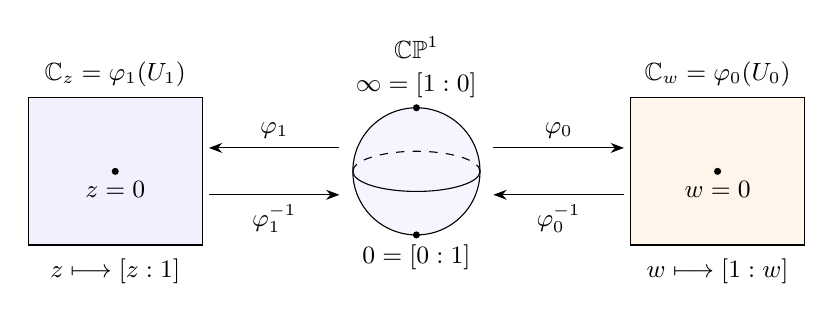
\begin{tikzpicture}[
  >=Stealth,
  scale=.85,
  every node/.style={font=\small}
]
% z 座標平面
\draw[fill=blue!6] (-5.8,-1.1) rectangle (-3.2,1.1);
\node at (-4.5,1.45) {$\C_z=\varphi_1(U_1)$};
\fill (-4.5,0) circle (1.5pt) node[below] {$z=0$};
\node at (-4.5,-1.5) {$z\longmapsto[z:1]$};

% w 座標平面
\draw[fill=orange!8] (3.2,-1.1) rectangle (5.8,1.1);
\node at (4.5,1.45) {$\C_w=\varphi_0(U_0)$};
\fill (4.5,0) circle (1.5pt) node[below] {$w=0$};
\node at (4.5,-1.5) {$w\longmapsto[1:w]$};

% Riemann 球面
\draw[fill=blue!4] (0,0) circle (.95);
\draw[dashed]
  (-.95,0) arc[start angle=180,end angle=0,
              x radius=.95,y radius=.3];
\draw
  (-.95,0) arc[start angle=180,end angle=360,
              x radius=.95,y radius=.3];

\fill (0,.95) circle (1.5pt)
  node[above] {$\infty=[1:0]$};
\fill (0,-.95) circle (1.5pt)
  node[below] {$0=[0:1]$};
\node at (0,1.85) {$\C\mathbb P^1$};

% 左：U_1 と C_z の対応
\draw[->] (-1.15,.35)--(-3.1,.35)
  node[midway,above] {$\varphi_1$};
\draw[->] (-3.1,-.35)--(-1.15,-.35)
  node[midway,below] {$\varphi_1^{-1}$};

% 右：U_0 と C_w の対応
\draw[->] (1.15,.35)--(3.1,.35)
  node[midway,above] {$\varphi_0$};
\draw[->] (3.1,-.35)--(1.15,-.35)
  node[midway,below] {$\varphi_0^{-1}$};

\end{tikzpicture}
\end{center}



\begin{rem}
\begin{itemize}
\item 上の補題において, 共通部分では $w=1/z$ が成り立つ.
なぜなら
$$
w= a_1/a_0 = (a_0/a_1)^{-1} = 1/z
$$
であるためである. 
従って, $\C\mathbb P^1$ は2枚の複素平面をこの関係で貼りあわせた空間であり, 球面 $S^2$ と同相なのでRiemann 球面と呼ばれる.
\item $\C\mathbb P^1$ で $\C{}_z$ に属さない点は $[1:0]$ のみであり, これを $\infty$ と書く.
$|z|\to\infty$ のとき $w=1/z\to 0$ となるので, この点は $\C{}_z$ の無限遠点とみなせる.
従って, $\C\mathbb P^1=\C{}_z\cup\{\infty\}$ は複素平面の一点コンパクト化である.これによっても球面 $S^2$ と同相がわかる. 
\end{itemize}
\end{rem}


商写像の性質から次がわかる. 
\begin{lem}\label{O-M006}
$X$ を位相空間とする. $f:\C\mathbb P^1\to X$ を $\C\mathbb P^1$ から $X$ への写像とする. このとき, $f$ が連続であることと $f\circ \pi:\C{}^2\setminus \{(0,0)\}\to X$ が連続であることは同値である. 
\end{lem}


これを使うと次がわかる. 
% SOURCE O:756 | O-M007 ques 1.3; original option: 1.3
\begin{lem}\label{O-M007}

\begin{itemize}

\item
\(
A=\begin{pmatrix}a&b\\ c&d\end{pmatrix}
\)
を複素可逆行列とする. このとき, 次の写像が定まる：
\[
p_A:\C\mathbb P^1\longrightarrow\C\mathbb P^1,\qquad
[a_0:a_1]\longmapsto[aa_0+ba_1:ca_0+da_1].
\]
代表元を非零定数倍しても像は変わらず, $A$ が可逆なので
右辺の二成分は同時に $0$ にならない.
逆写像は $p_{A^{-1}}$ であり, 補題 \ref{O-M006} より両者は連続である.
従って $p_A$ は同相写像である.
\item $F(X_0,X_1)\in \C{}[X_0,X_1]$ を同次多項式とする. $(F\neq 0):=\{p\in \C\mathbb P^1\mid F(p)\neq 0\}$ とおく. $(F\neq 0)$ は $\C\mathbb P^1$ の開集合である. 
\end{itemize}
\end{lem}

$z(\infty)=\infty$ と約束すると, 補題 \ref{O-M007} の同相写像 $p_A$ は非同次座標 $z$ を用いて
\[
z\longmapsto \frac{az+b}{cz+d}
\]
と表される.これはRiemann 球面上の一次分数変換である.



\begin{dfn}[写像の座標表示]
写像 $f:\C\mathbb P^1\to\C$ に対して,
\[
f_z:=f\circ\varphi_1^{-1}:\C_z\to\C,\qquad
f_w:=f\circ\varphi_0^{-1}:\C_w\to\C
\]
を, それぞれ $z$ 座標, $w$ 座標における
$f$ の座標表示という.
具体的には,
\[
f_z(z)=f([z:1]),\qquad f_w(w)=f([1:w])
\]
である.
\end{dfn}

\begin{exa}[同じ写像を二つの座標で表す]
写像
\[
f:\C\mathbb P^1\longrightarrow\C,\qquad
[a_0:a_1]\longmapsto
\frac{a_0\overline{a_1}}{|a_0|^2+|a_1|^2}
\]
を考える.
代表元を $\lambda$ 倍すると分子・分母がともに
$|\lambda|^2$ 倍されるので, この写像は矛盾なく定まる.

二つの座標表示は, それぞれ $[z:1]$, $[1:w]$ を代入して,
\[
f_z(z)=f([z:1])=\frac{z}{1+|z|^2},
\qquad
f_w(w)=f([1:w])=\frac{\overline w}{1+|w|^2}
\]
となる.
見た目は異なるが, 共通部分では$z=1/w$であり, 
\[
f_z(1/w)
=\frac{1/w}{1+1/|w|^2}
=\frac{\overline w}{1+|w|^2}
=f_w(w)
\]
であり, 同じ写像を表している.

また, 無限遠点は $w=0$ に対応するので,
\[
f(\infty)=f_w(0)=0
\]
と計算できる.
なお, この $f$ は連続写像であるが, 正則写像ではない.
\end{exa}


さて$\C\mathbb P^1$上の関数$\C\mathbb P^1\to \C$は商空間上の関数なのでわかりづらい. 
しかし次のことを頭に置いているとわかりやすいともう. 

\begin{lem}[座標表示の貼り合わせ]
写像 $f:\C\mathbb P^1\to\C$ の座標表示は,
\[
f_w(w)=f_z(1/w)\qquad(w\neq0)
\]
を満たす.

逆に, 写像 $f_z:\C_z\to\C$, $f_w:\C_w\to\C$ が
この関係を満たすならば,
これらを座標表示とする写像 $f:\C\mathbb P^1\to\C$ が
一意に存在する.
\[
\begin{tikzcd}[column sep=large,row sep=large]
\C_z^\times
\arrow[r,"z\mapsto1/z"]
\arrow[dr,"f_z"']
&
\C_w^\times
\arrow[d,"f_w"]
\\
&\C
\end{tikzcd}
\]
\end{lem}

\begin{proof}
$w\neq0$ ならば $[1:w]=[1/w:1]$ なので,
\[
f_w(w)=f([1:w])=f([1/w:1])=f_z(1/w).
\]

逆に, この関係が成り立つとき,
\[
f(p):=
\begin{cases}
f_z(\varphi_1(p)) & p\in U_1,\\
f_w(\varphi_0(p)) & p\in U_0
\end{cases}
\]
と定める.
共通部分では二つの値が一致するので, 矛盾なく定まる.
また, $U_0\cup U_1=\C\mathbb P^1$ より, $f$ は一意である.
\end{proof}

\begin{exa}
2つの連続関数
\[
f_z(z)=\frac{1}{1+|z|^2},\qquad
f_w(w)=\frac{|w|^2}{1+|w|^2}
\]
を考える.$w\neq 0$ のとき $f_w(w)=f_z(1/w)$ なので, 
これらは貼りあわさり, 連続関数 $f:\C\mathbb P^1\to\C$ を定める.
具体的には
\[
f([a_0:a_1])=\frac{|a_1|^2}{|a_0|^2+|a_1|^2}
\]
であり, $f([0:1])=1$, $f(\infty)=f([1:0])=0$ である.
\end{exa}


% SOURCE O:1029 | O-S011 複素平面領域及び $\C\mathbb P^1$ 上の正則関数と有理型関数
\subsection{複素解析の復習 -正則関数と有理型関数-}\label{O-S011-plane}


% SOURCE O:1035 | O-M015 defn 1.5; original option: 定義-命題 1.5
\begin{dfnprop}\label{O-M015}
$U$ を $\C{}_z$ の領域とする. $\varphi(z)$ を $U$ 上の複素数値関数とする. このとき, $\varphi(z)$ に関する次の $2$ つの条件は同値である：
\begin{enumerate}
\item
$\varphi(z)$ は $U$ の各点で正則, つまり$U$ の各点で複素微分可能, 同値できに
\[
\forall a\in U,\qquad \lim_{h\to 0}\frac{f(a+h)-f(a)}{h}\ \text{が複素数として存在する.}
\]
\item
$U$ の各点 $a$ の近傍で $\varphi(z)$ はTaylor級数展開できる.
\[
\varphi(z)=\sum_{n=0}^{\infty}\frac{\varphi^{(n)}(a)}{n!}(z-a)^n.
\]
%\item$U$ の任意の点 $a$ と $a$ を中心として $U$ に含まれる任意の開円板 $\Delta$ に対して, $\varphi(z)$ と $\varphi(z)$ の $a$ を中心とするTaylor級数展開は $\Delta$ 上一致する. すなわち, (2) の等式は $\Delta$ 全体で成立する等式である.
\end{enumerate}
\end{dfnprop}

複素解析でならった定理を思い出しておこう. 
\begin{thm}[一致の定理, 正則関数の剛性]\label{thm-identity-plane}
$U\subset\C$ を領域とし, $f,g:U\to\C$ を正則関数とする.
$U$ の空でない開部分集合上で $f=g$ ならば, $U$ 全体で $f=g$ である.
\end{thm}
\begin{thm}[Liouvilleの定理]
\label{thm-Liouville}
$\C$ 全体で正則な関数 $f:\C\to\C$ が有界ならば, $f$ は定数関数である.
\end{thm}

次に特異点にかんして思い出す. 


\begin{dfn}
$f$ を $0<|z-a|<r$ で正則な関数とする.
このとき $a$ を $f$ の孤立特異点といい, 次のように分類する.
\begin{enumerate}
\item $f(a)$ を適当に定めると $a$ でも正則になるとき, 
$a$ を除去可能特異点という.
\item
ある整数 $m\geq1$ と, $a$ の近傍で正則な関数 $h$ を用いて, 
$a$ の十分小さい穴あき近傍で
\[
f(z)=\frac{h(z)}{(z-a)^m},
\qquad h(a)\neq0
\]
と書けるとき, $a$ を $f$ の極といい, 
$m$ を極の位数という.
\item どちらでもないとき, $a$ を真性特異点という.
\end{enumerate}
除去可能特異点または極であることを, 高々極しかもたないという.
\end{dfn}

ラフに言えば, 「1は正則なのでどうでもよい, 2が今回の授業で扱う重要なもの, 3は難しすぎるので扱わない」である. 

\begin{thm}[Laurent展開]
$f$ が $0<|z-a|<r$ で正則ならば, この範囲で一意に
\[
f(z)=\sum_{n=-\infty}^{\infty}c_n(z-a)^n
\]
と展開できる.負の次数の項により, 特異点は次のように分類される.
\begin{enumerate}
\item 負の次数の項がすべて $0$：除去可能特異点.
\item 負の次数の項が有限個だけ非零：極.
このとき, 最も低い次数が $-m$ ならば $m$ 位の極という.
\item 負の次数の項が無限個非零：真性特異点.
\end{enumerate}
\end{thm}

\begin{exa}
$z=0$ における特異点を考える.
\begin{enumerate}
\item $\displaystyle \frac{\sin z}{z}
=1-\frac{z^2}{3!}+\frac{z^4}{5!}-\cdots$：
負の次数の項がないので, 除去可能特異点である.
\item $\displaystyle \frac{1+z}{z^2}=\frac{1}{z^2}+\frac{1}{z}$：
最も低い次数が $-2$ なので, $2$ 位の極である.
\item $\displaystyle e^{1/z}
=1+\frac{1}{z}+\frac{1}{2!z^2}+\cdots$：
負の次数の項が無限個非零なので, 真性特異点である.
\end{enumerate}
\end{exa}


\begin{dfn}
領域 $U$ 上で, 孤立した極を除いて正則な関数を
$U$ 上の有理型関数という.
ただし, 極は $U$ 内に集積点をもたないものとする.
\end{dfn}
\begin{exa}
$f(z)=1/(z-1)^2$ は $\C$ 上の有理型関数である.
$z=1$ に $2$ 位の極をもち, それ以外では正則である.
\end{exa}
\begin{exa}
$\tan z=\sin z/\cos z$ は $\C$ 上の有理型関数である.
$\cos z$ の零点 $z=\pi/2+k\pi$ $(k\in\Z)$ は単純零点であり,
その点で $\sin z\neq0$ なので, これらはすべて単純極である.
極は $\C$ 内に集積しない.
\end{exa}


% SOURCE O:1029 | O-S011 複素平面領域及び $\C\mathbb P^1$ 上の正則関数と有理型関数
\subsection{$\C\mathbb P^1$ 上の正則関数と有理型関数}\label{O-S011}

% SOURCE O:1088 | O-M018 defn 1.7; original option: 1.7
\begin{dfn}\label{O-M018}
$V$ を $\C\mathbb P^1$ の領域とする.
$f$ の $z$ 座標, $w$ 座標による表示を, それぞれ $f_z(z),f_w(w)$ とする.
\begin{enumerate}
\item $f_z(z),f_w(w)$ がそれぞれの定義域で正則であるとき, 
$f$ を $V$ 上の正則関数という.
\item $f_z(z),f_w(w)$ がそれぞれの座標領域で有理型であるとき, 
$f$ を $V$ 上の有理型関数という.
この場合, $f$ は極では定義されていなくてもよい.
\end{enumerate}
\end{dfn}

\begin{exa}
定数関数
\[
f:\C\mathbb P^1\longrightarrow\C,\qquad [a_0:a_1]\longmapsto1
\]
の座標表示は $f_z(z)=f([z:1])=1$, $f_w(w)=f([1:w])=1$ であり,
ともに正則である.

一方, 同次座標による商
\[
f([a_0:a_1])=\frac{a_0}{a_1}\qquad(a_1\neq0)
\]
を考えると,
\[
f_z(z)=z,\qquad f_w(w)=\frac1w
\]
となる. 従って $f$ は $\infty=[1:0]$ に単純極をもつ有理型関数である.
極では複素数値を取らないが, 値 $\infty$ を補うと
$[a_0:a_1]\mapsto[a_0:a_1]$ という $\C\mathbb P^1$ への写像になる.
\end{exa}

$\C\mathbb P^1$ で正則関数や有理型関数を考えるのだから, かなり難しいものがいっぱいあると予想されるが, 実は次のものしかない.



\begin{prop}\label{O-M022}
\begin{enumerate}
\item $\C\mathbb P^1$ 上の正則関数は定数関数に限る.つまり$\mathcal O_{\C\mathbb P^1}(\C\mathbb P^1)=\C{}$.
\item $\C\mathbb P^1$ 上の有理型関数は, $z$ の有理関数にほかならない.つまり$\mathcal M_{\C\mathbb P^1}(\C\mathbb P^1)=\C{}(z)$.
\end{enumerate}
\end{prop}

2つの多項式 $P(z),Q(z)$（$Q\not\equiv 0$）の商 $P(z)/Q(z)$ として表される関数を有理関数という.例えば$\frac{z}{z^2+1}$などである. 
ここで $\mathcal O_X(U)$, $\mathcal M_X(U)$ は, それぞれ
$U$ 上の正則関数, 有理型関数全体を表す.
これらを層として扱う意味は第 \ref{O-S032} 章で説明する.

\begin{proof}
(1) $f$ を $\C\mathbb P^1$ 上の正則関数とする.
$\C\mathbb P^1$ はコンパクトなので, 連続関数 $f$ は有界である.
従って, $f_z$ は有界な整関数であり, Liouvilleの定理\ref{thm-Liouville}から定数である.
無限遠点でも連続なので, $f$ は全体で定数である.

(2) 有理関数 $P(z)/Q(z)$ は, 有限の点では高々極しかもたない.
無限遠点でも, $w=1/z$ を代入した
$P(1/w)/Q(1/w)$ は $w$ の有理関数なので,
$w=0$ で高々極しかもたない.
従って, 球面全体の有理型関数を定める.

逆に, $f$ を球面上の有理型関数とする.
コンパクト性より極は有限個なので,
有限の極を $a_1,\ldots,a_s$,
その位数を $m_1,\ldots,m_s$ とする.
\[
Q(z):=\prod_{i=1}^s(z-a_i)^{m_i}
\]
とおけば, $Q$ の零点が $f$ の極を打ち消すので,
$F(z):=Q(z)f_z(z)$ は整関数となる.
有限の極がなければ $Q=1$ とする.

残る無限遠点でも $F$ は高々極しかもたないので,
$w=0$ の近くで
\[
F(1/w)
=\underbrace{\sum_{k=1}^m b_{-k}w^{-k}}_{\text{主要部}}
+\underbrace{H(w)}_{\text{$w=0$ で正則}}
\]
と書ける.
そこで, 多項式 $B(z):=\sum_{k=1}^m b_{-k}z^k$ を引くと,
\[
(F-B)(1/w)=H(w)
\]
となり, 無限遠点の極も消える.

従って, $F-B$ は球面全体で正則であり,
(1) より定数 $c$ である.
よって,
\[
f_z(z)=\frac{F(z)}{Q(z)}
=\frac{B(z)+c}{Q(z)}
\]
は有理関数である.
\end{proof}


\begin{cor}\label{O-M023}
同じ次数 $m$ の同次多項式 $F,G$ $(G\not\equiv0)$ に対して,
\[
f([a_0:a_1])=\frac{F(a_0,a_1)}{G(a_0,a_1)}
\]
は, 分母が非零の点で代表元によらず定まる.
この関数は球面全体の有理型関数に延長され,
すべての有理型関数はこの形で表される.
\end{cor}
\begin{proof}
$(a_0,a_1)$ を $(ca_0,ca_1)$ に替えても,
分子と分母の $c^m$ が打ち消し合う.
また, 座標表示は $F(z,1)/G(z,1)$ なので有理型である.

逆に, 命題 \ref{O-M022} より $f_z=P(z)/Q(z)$ と書ける.
$m=\max(\deg P,\deg Q)$ として
\[
F(X_0,X_1)=X_1^mP(X_0/X_1),\qquad
G(X_0,X_1)=X_1^mQ(X_0/X_1)
\]
とおけば, 両者は次数 $m$ の同次多項式であり, 求める表示を得る.
零関数の場合は $F=0$, $G=1$ とすればよい.
\end{proof}


% SOURCE O:1104 | O-M019 lem 1.8; original option: 補題-定義 1.8
\begin{lemdfn}[有理型関数の位数]\label{O-M019}
$V\subset\C\mathbb P^1$ を領域とし,
$f$ を $V$ 上の恒等的に零でない有理型関数とする.

\begin{itemize}
\item 有限の点 $p=[a:1]\in V$ では, 座標表示 $f_z$ は
\[
f_z(z)=(z-a)^m h(z),
\qquad m\in\Z,\quad h\text{ は }a\text{ の近くで正則},\quad h(a)\neq0
\]
と書ける.
この整数 $m$ は一意に定まり,
$f$ の $p$ における位数といい,
$\operatorname{ord}_p(f)$ と書く.
\item $\infty=[1:0]\in V$ では, $w=1/z$ による座標表示を用いて,
\[
f_w(w)=w^m h(w),
\qquad h\text{ は }0\text{ の近くで正則},\quad h(0)\neq0
\]
と書き, $\operatorname{ord}_\infty(f):=m$ と定める.
\end{itemize}

位数の意味は次のとおりである.
\[
\begin{array}{c|c}
\operatorname{ord}_p(f)>0 & \operatorname{ord}_p(f)\text{ 位の零点}\\
\operatorname{ord}_p(f)<0 & -\operatorname{ord}_p(f)\text{ 位の極}\\
\operatorname{ord}_p(f)=0 & \text{零点でも極でもない}
\end{array}
\]
また, $z,w$ の両方を使える点では,
どちらの座標表示で計算しても位数は一致する.
\end{lemdfn}

\begin{proof}
有理型関数のLaurent展開には負のべきが有限個しか現れない.
その最初の非零項を $c_m(z-a)^m$ とすると,
\[
f_z(z)=(z-a)^m
\underbrace{\bigl(c_m+c_{m+1}(z-a)+\cdots\bigr)}_{h(z)},
\qquad h(a)=c_m\neq0
\]
となる.
従って, $m$ は一意に定まる.
無限遠点でも $f_w$ の $w=0$ におけるLaurent展開を使えば同様である.

最後に, 両方の座標を使える点では $a\neq0$ である.
$b=1/a$ とおくと,
\[
z-a=\frac1w-a=-\frac aw(w-b)
\]
なので,
\[
f_w(w)=f_z(1/w)
=(w-b)^m
\underbrace{\left(-\frac aw\right)^m h(1/w)}_{b\text{ の近くで正則で, }b\text{ で非零}}.
\]
従って, $w$ 座標で計算しても位数は $m$ である.
\end{proof}

\begin{exa}[有理型関数の零点・極と位数]\label{O-M020}
$\C\mathbb P^1$ 上の有理型関数 $f$ を
\[
f_z(z)=\frac{z}{(z-1)^3}
\]
で定める.
無限遠点では, $w=1/z$ を用いて
\[
f_w(w)=f_z(1/w)
=\frac{1/w}{(1/w-1)^3}
=\frac{w^2}{(1-w)^3}
\]
と表示される.

補題・定義\ref{O-M019}に従い,
零点や極を表すべきと, その点で非零の正則関数とに分けると,
次の表を得る.
\[
\begin{array}{c|c|c|c}
p&\text{その点の近くでの表示}
&\operatorname{ord}_p(f)&\text{零点・極}\\ \hline
[0:1]
&z\,(z-1)^{-3}
&1&1\text{ 位の零点}\\[6pt]
[1:0]=\infty
&w^2\, (1-w)^{-3}
&2&2\text{ 位の零点}\\[6pt]
[1:1]
&(z-1)^{-3}\, z
&-3&3\text{ 位の極}
\end{array}
\]
これら以外の点では $f$ は正則かつ非零なので,
$\operatorname{ord}_p(f)=0$ である.
\end{exa}




% SOURCE O:1265 | O-S012 $\C\mathbb P^1$ から $\C\mathbb P^1$ への正則写像と $\C\mathbb P^1$ の等質性
\subsection{$\C\mathbb P^1$ から $\C\mathbb P^1$ への正則写像}\label{O-S012}


\begin{dfn}[正則写像]
$f:\C\mathbb P^1\to\C\mathbb P^1$ を連続写像とし,
$p\in\C\mathbb P^1$, $q=f(p)$ とする.
始域の座標を $z,w$, 終域の座標を $t,s$ とし,
$w=1/z$, $s=1/t$ とする.

\begin{enumerate}
\item
\textbf{$p\neq\infty$, $q\neq\infty$ の場合.}
座標表示
$F_1(z):=t(f([z:1]))$ が $z(p)$ の近くで正則であることをいう.

\item
\textbf{$p\neq\infty$, $q=\infty$ の場合.}
座標表示
$F_2(z):=s(f([z:1]))$ が $z(p)$ の近くで正則であることをいう.
ここでは, 終域の無限遠点を $s(\infty)=0$ として扱う.

\item
\textbf{$p=\infty$, $q\neq\infty$ の場合.}
座標表示
$F_3(w):=t(f([1:w]))$ が $w=0$ の近くで正則であることをいう.

\item
\textbf{$p=\infty$, $q=\infty$ の場合.}
座標表示
$F_4(w):=s(f([1:w]))$ が $w=0$ の近くで正則であることをいう.
\end{enumerate}

次の四つの場合に分けて, $f$ が $p$ で正則であることを定める.
図の $r$ は $p$ の近くを動く点を表す.
\begin{center}
\begin{tikzpicture}[
  scale=0.95,
  >=latex,
  every node/.style={font=\small},
  map/.style={->,thick},
  region/.style={draw=orange!80!black,fill=orange!15,thick}
]
% 始域
\path[draw=blue!60!black,fill=blue!5,thick]
  (-5,2.5)
  .. controls (-5.5,3.6) and (-4.5,4.2) .. (-3.4,3.9)
  .. controls (-2.2,4.4) and (-1.3,3.4) .. (-1.8,2.6)
  .. controls (-2.7,1.9) and (-4.3,2.1) .. cycle;
\node at (-3.5,4.45) {始域 $\C\mathbb P^1$};

\draw[region] (-3.5,3.05) ellipse (0.9 and 0.55);
\node at (-4.1,3.35) {$U$};
\fill (-3.5,3.05) circle (1.7pt) node[below right] {$p$};

% 終域
\path[draw=blue!60!black,fill=blue!5,thick]
  (1.8,2.6)
  .. controls (1.3,3.7) and (2.6,4.2) .. (3.6,3.9)
  .. controls (4.8,4.3) and (5.5,3.2) .. (5,2.5)
  .. controls (4,2.1) and (2.7,1.9) .. cycle;
\node at (3.5,4.45) {終域 $\C\mathbb P^1$};

\draw[region] (3.5,3.05) ellipse (0.9 and 0.55);
\node at (2.9,3.35) {$V$};
\fill (3.5,3.05) circle (1.7pt) node[below right] {$q=f(p)$};

% 多様体の間の写像
\draw[map] (-1.3,3.1) -- (1.3,3.1)
  node[midway,above] {$f$};
\node at (0,2.65) {$f(U)\subset V$};

% 下の二つの複素平面
\foreach \x in {-3.5,3.5}{
  \draw[draw=gray!60,fill=gray!4]
    (\x-1.45,-0.85) -- (\x+1.05,-0.85)
    -- (\x+1.45,0.85) -- (\x-1.05,0.85) -- cycle;
}

\draw[region] (-3.5,0) ellipse (0.85 and 0.5);
\node at (-4.05,0.3) {$\xi(U)$};
\fill (-3.5,0) circle (1.7pt) node[below right] {$\xi(p)$};
\node at (-3.5,-1.2) {$\C_\xi$};

\draw[region] (3.5,0) ellipse (0.85 and 0.5);
\node at (2.95,0.3) {$\eta(V)$};
\fill (3.5,0) circle (1.7pt) node[below right] {$\eta(q)$};
\node at (3.5,-1.2) {$\C_\eta$};

% 座標による表示
\draw[map] (-3.5,2.3) -- (-3.5,0.95)
  node[midway,left] {$\xi=z\text{ または }w$};
\draw[map] (3.5,2.3) -- (3.5,0.95)
  node[midway,right] {$\eta=t\text{ または }s$};

\draw[map] (-1.9,0) -- (1.9,0)
  node[midway,above] {$F=\eta\circ f\circ\xi^{-1}$}
  node[midway,below] {複素数の関数として正則};
\end{tikzpicture}
\end{center}


$f$ の連続性により, いずれの座標表示も
$p$ に対応する座標値の十分近くで定まる.
すべての点で正則である写像を正則写像という.
\end{dfn}

\begin{exa}
写像 $f:\C\mathbb P^1\to\C\mathbb P^1$ を
\[
f([X_0:X_1])=[X_0^2:X_1^2]
\]
と定める.
二成分は同時には零にならず, この写像は連続である.
$p\in\C\mathbb P^1$, $q=f(p)$ として,
四つの場合を確認する.

\begin{enumerate}
\item
\textbf{$p\neq\infty$, $q\neq\infty$ の場合.}
$f([z:1])=[z^2:1]$ なので, 座標表示は
\[
F_1(z)=t(f([z:1]))=z^2
\]
であり, すべての有限の点で正則である.

\item
\textbf{$p\neq\infty$, $q=\infty$ の場合.}
有限の点の像は $[z^2:1]$ であり,
$\infty=[1:0]$ にはならない.
従って, この場合は起こらない.

\item
\textbf{$p=\infty$, $q\neq\infty$ の場合.}
$f([1:0])=[1:0]$ なので,
この場合も起こらない.

\item
\textbf{$p=\infty$, $q=\infty$ の場合.}
$f([1:w])=[1:w^2]$ なので, 座標表示は
\[
F_4(w)=s(f([1:w]))=w^2
\]
であり, $w=0$ でも正則である.
\end{enumerate}

従って, $f$ は $\C\mathbb P^1$ 全体で正則な写像である.
\end{exa}

\begin{exa}
写像 $f:\C\mathbb P^1\to\C\mathbb P^1$ を
\[
f([X_0:X_1])=[X_1:X_0-X_1]
\]
と定める.
二成分は同時には零にならず, この写像は連続である.
有限部分では $f(z)=1/(z-1)$ と表示され,
$f(1)=\infty$, $f(\infty)=0$ である.

$p\in\C\mathbb P^1$, $q=f(p)$ として,
四つの場合を確認する.

\begin{enumerate}
\item
\textbf{$p\neq\infty$, $q\neq\infty$ の場合.}
この場合は $z(p)\neq1$ である.
$f([z:1])=[1:z-1]$ なので, 座標表示は
\[
F_1(z)=t(f([z:1]))=\frac1{z-1}
\]
であり, $z(p)$ の近くで正則である.

\item
\textbf{$p\neq\infty$, $q=\infty$ の場合.}
この場合は $p=[1:1]$, すなわち $z(p)=1$ である.
終域の $s$ 座標を使うと,
\[
F_2(z)=s(f([z:1]))=z-1
\]
となり, $z=1$ でも正則である.

\item
\textbf{$p=\infty$, $q\neq\infty$ の場合.}
$f(\infty)=0$ である.
$f([1:w])=[w:1-w]$ なので, 座標表示は
\[
F_3(w)=t(f([1:w]))=\frac{w}{1-w}
\]
であり, $w=0$ の近くで正則である.

\item
\textbf{$p=\infty$, $q=\infty$ の場合.}
$f(\infty)=0$ なので, この場合は起こらない.
\end{enumerate}

従って, $f$ は $\C\mathbb P^1$ 全体で正則な写像である.
特に, 有理関数として極をもつ $z=1$ でも,
終域の $s$ 座標を使えば正則に表示される.
\end{exa}

\begin{thm}[正則写像と有理関数]
次の対応により, $\C\mathbb P^1$ 上の有理型関数と,
定値写像 $f\equiv\infty$ を除く正則写像
$f:\C\mathbb P^1\to\C\mathbb P^1$ は一対一に対応する.
\[
R\longmapsto f,\qquad
f(p)=
\begin{cases}
[R(p):1] & p\text{ が }R\text{ の極でないとき},\\
[1:0]=\infty & p\text{ が }R\text{ の極のとき}.
\end{cases}
\]
すなわち, 有理型関数の極に値 $\infty$ を与えると正則写像になり,
逆に, 正則写像の値を終域の有限座標で読み取ると有理型関数になる.

さらに, 命題\ref{O-M022}より,
これらの有理型関数はすべて有理関数 $R(z)\in\C(z)$ である.
\end{thm}

\begin{proof}
終域の座標を $t,s$ とし, $s=1/t$ とする.

\textbf{(1) 有理型関数から正則写像を作る.}

$R$ が正則な点では, 終域の $t$ 座標による表示が
$R$ そのものなので, $f$ は正則である.

有限の点 $p=[a:1]$ が $R$ の $m$ 位の極ならば,
補題・定義\ref{O-M019}より,
\[
R_z(z)=\frac{h(z)}{(z-a)^m},
\qquad h\text{ は正則},\quad h(a)\neq0
\]
と書ける.
このとき, 終域の $s$ 座標による表示は
\[
s(f([z:1]))=\frac1{R_z(z)}
=\frac{(z-a)^m}{h(z)}.
\]
右辺は $z=a$ でも正則で, 値は $0=s(\infty)$ である.
従って, 極に値 $\infty$ を与えた $f$ は,
$p$ でも連続かつ正則である.

無限遠点でも, $R_w(w)$ を用いれば同様である.
実際, $R_w(w)=h(w)/w^m$ ならば,
$s(f([1:w]))=w^m/h(w)$ は $w=0$ で正則となる.
よって, $f$ は球面全体で正則である.

\medskip
\noindent
\textbf{(2) 正則写像から有理型関数を取り出す.}

$f\not\equiv\infty$ を正則写像とする.
$f(p)\neq\infty$ のところで
\[
R(p):=t(f(p))
\]
と定める.
正則写像の定義より, $R$ はそこで正則である.

有限の点 $p=[a:1]$ で $f(p)=\infty$ となる場合を考える.
終域の $s$ 座標による表示
\[
G(z):=s(f([z:1]))
\]
は $a$ の近くで正則であり, $G(a)=0$ である.
また, $f\not\equiv\infty$ なので,
一致の定理より $G$ は恒等的には零でない.
\footnote{
もし $f$ がある開集合上で恒等的に $\infty$ ならば,
その性質は一致の定理によって球面全体に広がる.
実際, $f$ が近傍上で恒等的に $\infty$ となる点の集合は開集合であり,
その極限点でも $s\circ f$ に一致の定理を適用すれば同じ性質が成り立つ.
従ってこの集合は閉集合でもあり, 球面の連結性から全体となる
（定理\ref{thm-identity-plane}参照）.
}
従って,
\[
G(z)=(z-a)^m h(z),
\qquad m\geq1,\quad h(a)\neq0
\]
と書けるので,
\[
R_z(z)=\frac1{G(z)}
=\frac1{(z-a)^m h(z)}
\]
は $a$ に $m$ 位の極をもつ.
無限遠点でも $w$ 座標を使えば同様である.

こうして得た二つの表示は, 共通部分で
\[
R_w(w)=R_z(1/w)
\]
を満たすので, 球面上の有理型関数 $R$ を定める.
この $R$ に (1) の操作を施すと, もとの写像 $f$ に戻る.
また, $R$ は $f$ の有限の値から決まるので一意である.
\end{proof}

\begin{dfn}[自己同型]
正則写像 $f:\C\mathbb P^1\to\C\mathbb P^1$ が全単射で, 
逆写像 $f^{-1}$ も正則であるとき, $f$ を $\C\mathbb P^1$ の自己同型という.
自己同型全体は合成について群をなし, これを
$\operatorname{Aut}(\C\mathbb P^1)$ と書く.
\end{dfn}

\begin{lem}[一次分数変換と等質性]
一次分数変換
\[
z\longmapsto\frac{az+b}{cz+d},\qquad ad-bc\neq0
\]
は $\C\mathbb P^1$ の自己同型である.
また, 任意の $p,q\in\C\mathbb P^1$ に対して, 
$p$ を $q$ に移す一次分数変換が存在する.
\end{lem}

\begin{proof}
\textbf{(1) 一次分数変換は自己同型である.}

$f(z)=(az+b)/(cz+d)$ は有理関数なので,
前の定理より $\C\mathbb P^1$ への正則写像を定める.
その逆写像は
\[
g(t)=\frac{dt-b}{-ct+a}
\]
であり, これも有理関数なので正則写像を定める.
実際, 分母が零でないところで計算すると,
\[
g(f(z))
=\frac{d(az+b)-b(cz+d)}{-c(az+b)+a(cz+d)}
=\frac{(ad-bc)z}{ad-bc}=z.
\]
同様に $f(g(t))=t$ であり,
残りの点でも連続性により成り立つ.
従って, $f$ は正則な逆写像をもつので自己同型である.

\medskip
\noindent
\textbf{(2) 任意の点を任意の点に移せる.}

各点 $p$ に対して, $p$ を $0$ に移す一次分数変換を
\[
T_p(z):=
\begin{cases}
z-p & p\neq\infty,\\
1/z & p=\infty
\end{cases}
\]
と定める.
このとき,
\[
p\xmapsto{\ T_p\ }0\xmapsto{\ T_q^{-1}\ }q
\]
なので, $T_q^{-1}\circ T_p$ が求める変換である.
一次分数変換の逆写像と合成も一次分数変換である.
\end{proof}

後半の性質を $\C\mathbb P^1$ の等質性という.
これは, 無限遠点も有限の点も, 自己同型によって互いに移せることを意味する.
特に, 指定された有限個の点以外の点を $\infty$ に移せば, 
指定された点をすべて有限の点として扱える.

\begin{thm}[自己同型の分類]
\label{thm-aut-projective-line}
$\C\mathbb P^1$ の自己同型は, ちょうど一次分数変換
\[
z\longmapsto\frac{az+b}{cz+d},\qquad ad-bc\neq0
\]
である.
\end{thm}
\begin{proof}
一次分数変換が自己同型であることは, 直前の補題で示した.
逆に, 自己同型 $f$ が一次分数変換であることを示す.

直前の補題より, $f(\infty)$ を $\infty$ に移す
一次分数変換 $T$ を取れる.
このとき,
\[
g:=T\circ f,\qquad g(\infty)=\infty
\]
であり, $g$ も自己同型である.

$g$ は全単射なので, 有限の点を $\infty$ に移すことはない.
従って, $g$ は有限の点に極をもたない有理関数であり,
多項式である（命題\ref{O-M022}とその証明参照）.
逆写像 $h:=g^{-1}$ も $\infty$ を固定するので,
同じ理由で多項式である.

$g,h$ の次数をそれぞれ $m,n\geq1$ とすると,
\[
1
=\deg (h\circ g)
\underalign{\text{(多項式の合成の次数)}}{=}
nm.
\]
ここで, 次数 $n$ の多項式に次数 $m$ の多項式を代入すると,
最高次の項は次数 $nm$ となることを使った.
従って $m=n=1$ であり,
$g(z)=az+b$ $(a\neq0)$ と書ける.

よって, $f=T^{-1}\circ g$ は一次分数変換の合成なので,
一次分数変換である.
\end{proof}




最後に, 極の位置と位数を制限した有理型関数を考える.


\begin{prop}
\label{prop-RR-projective}
$p\in\C\mathbb P^1$ と非負整数 $n$ を固定する.
$p$ に高々 $n$ 位の極をもち, それ以外に極をもたない
有理型関数全体を $L$ とする.
このとき $L$ は複素線形空間であり, 次が基底となる：
\[
\begin{cases}
1,\ \dfrac1{z-a},\ \ldots,\ \dfrac1{(z-a)^n}
& (p=[a:1]),\\[6pt]
1,\ z,\ \ldots,\ z^n
& (p=\infty).
\end{cases}
\]
従って $\dim_{\C}L=n+1$ である.
\end{prop}

\begin{proof}
$p=[a:1]$ の場合, $f\in L$ の $a$ でのLaurent展開を
\[
f(z)=\sum_{k=1}^{n}\frac{c_{-k}}{(z-a)^k}
     +\sum_{j=0}^{\infty}c_j(z-a)^j
\]
とする.負の次数の項を引いた関数
\[
h(z)=f(z)-\sum_{k=1}^{n}\frac{c_{-k}}{(z-a)^k}
\]
は $a$ で正則に延長され, それ以外の有限の点でも正則である.
また, 引いた各項は $z\to\infty$ で $0$ に近づき, 
無限遠点でも正則なので, $h$ は $\C\mathbb P^1$ 全体で正則である.
従って $h$ は定数 $C$ であり, 
\[
f(z)=C+\sum_{k=1}^{n}\frac{c_{-k}}{(z-a)^k}
\]
と書ける.
\end{proof}


一般には次のようになる. これはあとでやるRiemann--Rochの具体例である.
\begin{prop}
$p_1,\ldots,p_m$ を $\C\mathbb P^1$ の異なる点とし, 
$n_1,\ldots,n_m$ を非負整数とする.
$p_i$ に高々 $n_i$ 位の極をもち, それ以外に極をもたない
有理型関数全体を $L$ とおく.
このとき $L$ は複素線形空間であり, 
\[
\dim_{\C}L=1+\sum_{i=1}^{m}n_i.
\]
\end{prop}

\newpage

% SOURCE O:1414 | O-S013 Riemann 面と正則写像
\section{Riemann 面と正則写像}\label{O-S013}
Riemann 面の抽象的な理論を見ていく. わからない場合はしばらくRiemann 面を$\C\mathbb P^1$だと思っても良い. 

% SOURCE O:1418 | O-S014 Riemann 面の定義と付随するいくつかの概念
\subsection{Riemann 面の定義}\label{O-S014}

以下では, 座標写像を $\varphi:U\to V\subset\C$,
複素平面 $V$ の変数を $z$ と書く.
点 $p\in U$ の座標値は $\varphi(p)$ と書き,
点そのものと座標値を区別する.

% SOURCE O:1422 | O-M035 defn 2.1; original option: 2.1
\begin{dfn}\label{O-M035}
次の条件 (1)--(4) をみたす対
\[
\left(X,\{\varphi_i:U_i\to V_i\}_{i\in I}\right)
\]
のことを, 位相空間 $X$ を台空間とし $\{\varphi_i:U_i\to V_i\}_{i\in I}$ をアトラスとするRiemann 面という.
\begin{enumerate}
\item
$X$ は空でない第 $2$ 可算公理をみたす連結Hausdorff空間である.
\item
各 $i\in I$ に対して $U_i$ は $X$ の空でない開集合でありかつ $X=\bigcup_{i\in I}U_i$ が成り立つ. すなわち, $\{U_i\}_{i\in I}$ は $X$ の開被覆である.
\item
各 $i\in I$ に対して $V_i$ は $\C{}_{z_i}$ の開集合でありかつ $\varphi_i:U_i\to V_i$ は同相写像である.
\item
$U_i\cap U_j\neq \emptyset$ である任意の $(i,j)\in I^2$ に対して $V_{ij}:=\varphi_j(U_i\cap U_j)\subset V_j$ とおく. このとき, (3) から定まる写像
\[
\varphi_{ij}:=\varphi_i\circ \varphi_j^{-1}|_{V_{ij}}:V_{ij}\to V_{ji}
\]
は正則写像である.
\end{enumerate}
\[
\begin{tikzcd}[column sep=large,row sep=large]
& U_i\cap U_j \arrow[dl,"\varphi_j"'] \arrow[dr,"\varphi_i"] &\\
V_{ij} \arrow[rr,"\varphi_i\circ\varphi_j^{-1}"'] && V_{ji}
\end{tikzcd}
\]
上段は $X$ の開集合, 下段は $\C$ の開集合である.
座標変換は同じ点を二通りの複素数で表す対応である.
アトラスの元のことを座標近傍系といい, しばしば $(\varphi_i,U_i)$ と略記して書く.

\end{dfn}
細かいことを言うと"第 $2$ 可算公理"や"連結"を仮定しない定義もある.\footnote{位相空間 $X$ が第二可算公理を満たすとは, 可算個の開集合からなる族 $\{U_n\}_{n\in\mathbb N}$ が存在し, 
$X$ の任意の開集合がこれらの合併として表されることをいう.}
が面倒なのでこの定義でいく\footnote{1の分割とか色々できるのが第 $2$ 可算公理と思って良い. 松本幸夫の多様体の基礎ではこの辺りがかなり詳しいが, 最近の教科書は多様体に第 $2$ 可算公理を仮定することが多いと思う. 連結は人による. 私は多様体は第二可算, 連結, 向き付け可能, $C^\infty$級を常に仮定する. Riemann 面(複素多様体)は向き付け可能である. }

\begin{exa}\label{O-M036}
$\C{}$ の領域 $U$ は $\{id:U\to U\}$ をアトラスとするRiemann 面である.
\end{exa}

\begin{exa}
$\C\mathbb P^1$ は, 2つの座標近傍
$(\varphi_0,U_0),(\varphi_1,U_1)$ をアトラスとする
コンパクトRiemann 面である.実際, 定義の各条件を確認すると：
\begin{enumerate}
\item $\C\mathbb P^1$ は球面 $S^2$ と同相なので, 
空でない第2可算な連結Hausdorff空間である.

\item
\[
U_0=\{[X_0:X_1]\mid X_0\neq0\},\qquad
U_1=\{[X_0:X_1]\mid X_1\neq0\}
\]
は空でない開集合であり, $\C\mathbb P^1=U_0\cup U_1$ である.

\item 既に示したように, 
\[
\varphi_0:U_0\to\C_w,\quad [X_0:X_1]\mapsto\frac{X_1}{X_0},
\qquad
\varphi_1:U_1\to\C_z,\quad [X_0:X_1]\mapsto\frac{X_0}{X_1}
\]
は同相写像であり, その像 $\C_w,\C_z$ は複素平面の開集合である.

\item 共通部分の座標像は, いずれも $\C\setminus\{0\}$ であり, 
座標変換は
\[
\varphi_0\circ\varphi_1^{-1}(z)=\frac1z,\qquad
\varphi_1\circ\varphi_0^{-1}(w)=\frac1w
\]
となる.これらは定義域上で正則である.
同じ座標間の変換は恒等写像なので, やはり正則である.
\end{enumerate}
従って $\C\mathbb P^1$ はRiemann 面であり, 
さらに $S^2$ と同相なのでコンパクトである.
\end{exa}

% SOURCE O:1614 | O-M047 defn 2.10; original option: 2.10
\begin{dfn}[点を中心とする局所座標]\label{O-M047}
$p\in X$ の座標近傍 $(\varphi,U)$ が $\varphi(p)=0$ を満たすとき,
これを $p$ を中心とする局所座標近傍系という.
このとき $\varphi$ を $p$ での局所座標と呼ぶ.
任意の座標写像 $\psi$ から $\varphi=\psi-\psi(p)$ とすれば,
常にこのような座標が得られる.
\end{dfn}


% SOURCE O:1500 | O-M038 defn 2.4; original option: 2.4
\begin{dfn}[正則写像と正則関数]
\label{O-M038}
$X,Y$ をRiemann 面, $f:X\to Y$ を連続写像とする.
$p\in X$ の座標近傍 $(\varphi,U)$ と $f(p)\in Y$ の座標近傍
$(\psi,V)$ を取り, 必要なら $U$ を小さくして $f(U)\subset V$ とする.
このとき, 座標表示
\[
F=\psi\circ f\circ\varphi^{-1}:\varphi(U)\longrightarrow\psi(V)
\]
が $\varphi(p)$ の近くで正則ならば, $f$ は $p$ で正則であるという.
すべての点で正則な写像を正則写像という.
\begin{center}
\begin{tikzpicture}[
  scale=0.95,
  >=latex,
  every node/.style={font=\small},
  map/.style={->,thick},
  region/.style={draw=orange!80!black,fill=orange!15,thick}
]
% 始域 X
\path[draw=blue!60!black,fill=blue!5,thick]
  (-5,2.5)
  .. controls (-5.5,3.6) and (-4.5,4.2) .. (-3.4,3.9)
  .. controls (-2.2,4.4) and (-1.3,3.4) .. (-1.8,2.6)
  .. controls (-2.7,1.9) and (-4.3,2.1) .. cycle;
\node at (-3.5,4.45) {Riemann 面 $X$};

\draw[region] (-3.5,3.05) ellipse (0.9 and 0.55);
\node at (-4.05,3.3) {$U$};
\fill (-3.5,3.05) circle (1.7pt)
  node[below right] {$p$};

% 終域 Y
\path[draw=blue!60!black,fill=blue!5,thick]
  (1.8,2.6)
  .. controls (1.3,3.7) and (2.6,4.2) .. (3.6,3.9)
  .. controls (4.8,4.3) and (5.5,3.2) .. (5,2.5)
  .. controls (4,2.1) and (2.7,1.9) .. cycle;
\node at (3.5,4.45) {Riemann 面 $Y$};

\draw[region] (3.5,3.05) ellipse (0.9 and 0.55);
\node at (2.95,3.3) {$V$};
\fill (3.5,3.05) circle (1.7pt)
  node[below right] {$f(p)$};

% Riemann 面の間の写像
\draw[map] (-1.3,3.1) -- (1.3,3.1)
  node[midway,above] {$f$};
\node at (0,2.65) {$f(U)\subset V$};

% 二つの複素平面
\foreach \x in {-3.5,3.5}{
  \draw[draw=gray!60,fill=gray!4]
    (\x-1.45,-0.85) -- (\x+1.05,-0.85)
    -- (\x+1.45,0.85) -- (\x-1.05,0.85) -- cycle;
}

\draw[region] (-3.5,0) ellipse (1 and 0.55);
\node at (-3.85,0.3) {$\varphi(U)$};
\fill (-3.5,0) circle (1.7pt)
  node[below right] {$\varphi(p)$};
\node at (-3.5,-1.2) {$\C$};

\draw[region] (3.5,0) ellipse (1 and 0.55);
\node at (3.15,0.3) {$\psi(V)$};
\fill (3.5,0) circle (1.7pt)
  node[below right] {$\psi(f(p))$};
\node at (3.5,-1.2) {$\C$};

% 座標写像
\draw[map] (-3.5,2.3) -- (-3.5,0.95)
  node[midway,left] {座標写像 $\varphi$};
\draw[map] (3.5,2.3) -- (3.5,0.95)
  node[midway,right] {座標写像 $\psi$};

% 座標表示
\draw[map] (-1.9,0) -- (1.9,0)
  node[midway,above] {$F=\psi\circ f\circ\varphi^{-1}$}
  node[midway,below,align=center]
    {$\varphi(p)$ の近くで\\正則性を調べる};
\end{tikzpicture}
\end{center}


\end{dfn}
つまり, 複素平面の開集合間の関数に直して正則性を調べる.
特に, 終域が $\C$ の場合を正則関数という.
開集合 $U\subset X$ 上の関数についても, 各点で同じ条件を課す.


\begin{exa}[$z^2$ が定める正則写像]
写像 $f:\C\mathbb P^1\to\C\mathbb P^1$ を
\[
f([X_0:X_1])=[X_0^2:X_1^2]
\]
と定める.
これは連続写像であり, 有限部分では $f(z)=z^2$,
無限遠点では $f(\infty)=\infty$ である.

始域の座標を $z,w$, 終域の座標を $t,s$ とし,
$w=1/z$, $s=1/t$ とする.
定義\ref{O-M038}の座標表示は次のようになる.
\[
\begin{array}{c|c|c|c}
\text{調べる点 }p&\varphi&\psi&
F=\psi\circ f\circ\varphi^{-1}\\ \hline
p\neq\infty&z&t&z\longmapsto z^2\\[2pt]
p=\infty&w&s&w\longmapsto w^2
\end{array}
\]
実際, $f([z:1])=[z^2:1]$,
$f([1:w])=[1:w^2]$ から, これらの表示が得られる.
いずれも正則なので, $f$ は正則写像である.
\end{exa}

\begin{exa}[$1/(z-1)$ が定める正則写像]
写像 $f:\C\mathbb P^1\to\C\mathbb P^1$ を
\[
f([X_0:X_1])=[X_1:X_0-X_1]
\]
と定める.
これは連続写像であり,
\[
f(z)=\frac1{z-1}\quad(z\neq1,\infty),
\qquad f(1)=\infty,\qquad f(\infty)=0
\]
である.

前の例と同じ座標を用いると, 座標表示は次のようになる.
\[
\begin{array}{c|c|c|c}
\text{調べる点 }p&\varphi&\psi&
F=\psi\circ f\circ\varphi^{-1}\\ \hline
p\neq1,\infty&z&t&z\longmapsto\dfrac1{z-1}\\[6pt]
p=1&z&s&z\longmapsto z-1\\[2pt]
p=\infty&w&t&w\longmapsto\dfrac{w}{1-w}
\end{array}
\]
実際, $f([z:1])=[1:z-1]$ なので,
終域の $t$ 座標では $1/(z-1)$,
$s$ 座標では $z-1$ と表示される.
また, $f([1:w])=[w:1-w]$ から,
最後の表示が得られる.

各表示は, それぞれ調べる点の座標値の近くで正則なので,
$f$ は正則写像である.
特に, $1/(z-1)$ は $z=1$ に極をもつが,
終域の $s$ 座標を使えば, 写像はその点でも正則に表示される.
\end{exa}

複素解析の時と同じく, Riemann 面でも一致の定理が成り立つ. 
% SOURCE O:1762 | O-M053 thm 2.14; original option: 2.14
\begin{thm}[一致の定理]\label{O-M053}
Riemann 面間の正則写像 $f,g:X\to Y$ が空でない開集合上で一致すれば, 
$X$ 全体で一致する.
特に, 空でない開集合上で定値な正則写像は, 全体で定値である.
\end{thm}

\begin{proof}
\[
Z=\{p\in X\mid p\text{ のある近傍で }f=g\}
\]
とおく.仮定と定義から, $Z$ は空でない開集合である.

$Z$ が閉集合であることを示すため, $p\in\overline Z$ を取る.
一致点の集合
\[
E=\{q\in X\mid f(q)=g(q)\}
\]
は下の補題より閉集合であり, $Z\subset E$ なので
$\overline Z\subset E$ である.従って $f(p)=g(p)$ となる.


$q=f(p)=g(p)$ とし, $Y$ の $q$ を含む座標近傍 $(\psi,V)$ を取る.
$f,g$ の連続性より, $X$ の $p$ を含む連結な座標近傍 $(\varphi,U)$ を
\[
f(U)\subset V,\qquad g(U)\subset V
\]
となるように選べる.

この座標による表示
\[
F=\psi\circ f\circ \varphi^{-1},\qquad
G=\psi\circ g\circ \varphi^{-1}
\]
は, 複素平面の領域 $\varphi(U)$ 上の正則関数である.
$p\in\overline Z$ より $U\cap Z$ は空でない開集合であり, 
その上で $f=g$ なので, 
\[
F=G\qquad\text{on }\varphi(U\cap Z)
\]
が成り立つ.
複素平面での一致の定理から, $\varphi(U)$ 全体で $F=G$ となる.
従って $U$ 上で $\psi\circ f=\psi\circ g$ であり, 
$\psi$ は単射なので $f=g$ である.
従って, $p$ の近傍で $f=g$ となるので $p\in Z$ である.
よって $\overline Z\subset Z$ であり, $Z$ は閉集合である.

以上より$X$ は連結なので $Z=X$ となり, $f=g$ を得る.
最後の主張は $g$ を定値写像とすれば従う.
\end{proof}

% SOURCE O:1781 | O-M054 ques 2.6; original option: 2.6
\begin{lem}\label{O-M054}
$A$ を位相空間, $B$ をHausdorff空間とする.
$f, g : A\to B$が連続ならば
\(
\{a\in A\mid f(a)=g(a)\}
\)
は $A$ の閉集合である. 
\end{lem}

\subsection{コンパクトRiemann 面の正則同型と位相同型の違い}

\begin{dfn}[双正則写像]\label{O-M040}
$X,Y$ をRiemann 面とする.
正則写像 $f:X\to Y$ が正則な逆写像 $g:Y\to X$ をもつとき,
すなわち
\[
g\circ f=\operatorname{id}_X,\qquad
f\circ g=\operatorname{id}_Y
\]
を満たすとき, $f$ を双正則写像という.
このような写像が存在するとき,
$X,Y$ は双正則同型である, または単に同型であるといい,
$X\simeq Y$ と書く.
\end{dfn}

Riemann 面の位相的な構造に関しては次がわかっている.
\begin{itemize}
\item  Riemann 面は自然に実2次元の $C^\infty$ 級多様体となる.
(これがRiemann「面」と呼ぶ理由である.)
これはRiemann 面の複素座標 $z_i=x_i+\sqrt{-1}y_i$ を
実座標 $(x_i,y_i)$ とみなせるためである. 
\item  Riemann 面は向き付け可能である.
これは, 複素座標の変換が実平面の向きを保つことによる. （補題\ref{O-M098}とその後の補足参照）.
\end{itemize}

従って, コンパクトRiemann 面には曲面の分類定理を適用できる.
第4章の定理\ref{O-M174}で扱う結果のうち,
ここでは曲面の形に関する結論を先に紹介する.

\begin{thm}[向き付け可能な閉曲面の分類]
$\Sigma_g$ を, 球面に $g$ 個の取っ手を付けた曲面とする.
連結かつ向き付け可能なコンパクトで境界をもたない実2次元曲面は,
ただ一つの非負整数 $g$ に対して $\Sigma_g$ と同相である.

特に, 任意のコンパクトRiemann 面は,
球面にいくつかの取っ手を付けた曲面と同相である.
\end{thm}

\begin{figure}[htbp]
\centering
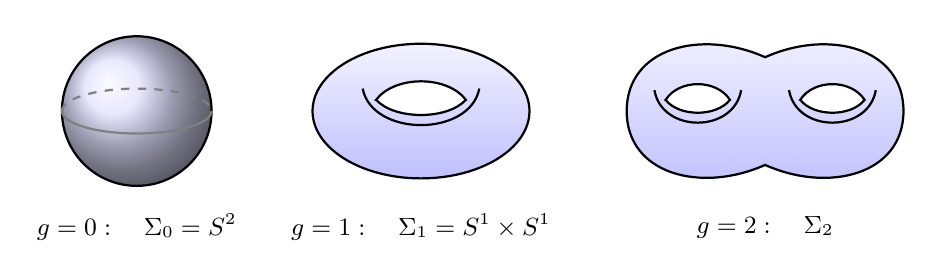
\begin{tikzpicture}[
  scale=0.95,
  line width=0.8pt,
  every node/.style={font=\small}
]
% 種数 0
\begin{scope}
  \shade[ball color=blue!12] (0,0) circle (1);
  \draw (0,0) circle (1);
  \draw[dashed,gray]
    (-1,0) arc[start angle=180,end angle=0,
              x radius=1,y radius=0.3];
  \draw[gray]
    (-1,0) arc[start angle=180,end angle=360,
              x radius=1,y radius=0.3];
  \node at (0,-1.55) {$g=0:\quad\Sigma_0=S^2$};
\end{scope}

% 種数 1
\begin{scope}[shift={(3.8,0)}]
  \shade[top color=blue!5,bottom color=blue!25]
    (0,0) ellipse[x radius=1.45,y radius=0.9];
  \draw (0,0) ellipse[x radius=1.45,y radius=0.9];

  \filldraw[fill=white]
    (-0.6,0.15)
    .. controls (-0.35,0.48) and (0.35,0.48) .. (0.6,0.15)
    .. controls (0.35,-0.12) and (-0.35,-0.12) .. cycle;
  \draw
    (-0.78,0.30)
    .. controls (-0.65,-0.35) and (0.65,-0.35) .. (0.78,0.30);

  \node at (0,-1.55)
    {$g=1:\quad\Sigma_1=S^1\times S^1$};
\end{scope}

% 種数 2
\begin{scope}[shift={(8.4,0)}]
  \path[shade,top color=blue!5,bottom color=blue!25,draw=black]
    (-1.85,0)
    .. controls (-1.85,0.85) and (-0.85,1.10) .. (0,0.72)
    .. controls (0.85,1.10) and (1.85,0.85) .. (1.85,0)
    .. controls (1.85,-0.85) and (0.85,-1.10) .. (0,-0.72)
    .. controls (-0.85,-1.10) and (-1.85,-0.85) .. cycle;

  \foreach \a in {-0.9,0.9}{
    \begin{scope}[shift={(\a,0)}]
      \filldraw[fill=white]
        (-0.43,0.15)
        .. controls (-0.25,0.43) and (0.25,0.43) .. (0.43,0.15)
        .. controls (0.25,-0.08) and (-0.25,-0.08) .. cycle;
      \draw
        (-0.58,0.28)
        .. controls (-0.48,-0.30) and (0.48,-0.30) .. (0.58,0.28);
    \end{scope}
  }
  \node at (0,-1.55) {$g=2:\quad\Sigma_2$};
\end{scope}
\end{tikzpicture}
\caption{取っ手の個数が $0,1,2$ の閉曲面の模式図.}
\label{fig-surfaces-topological-preview}
\end{figure}

$X$ が $\Sigma_g$ と同相であるとき,
$g$ を $X$ の位相的種数という. つまり, 位相的種数は取っ手の個数である.
後に, コホモロジーを用いて解析的種数を定義し,
それがこの取っ手の個数と一致することを示す
（定理\ref{O-M305}参照）.

ただし, 二つのRiemann 面が滑らかな曲面として微分同相であっても,
双正則同型であるとは限らない.
例えば, 複素トーラスはすべて滑らかな曲面としては
$S^1\times S^1$ と微分同相だが,
互いに双正則同型とは限らない.
このように, 同じ滑らかな曲面上の複素構造を
双正則同型の違いを除いて分類することが,
モジュライの問題につながる.
具体例は後に説明する（補足\ref{O-M360}参照）.


% SOURCE O:1758 | O-S015 Riemann 面からRiemann 面への正則写像の性質
\subsection{有理型関数とorder}\label{O-S015}


% SOURCE O:1816 | O-M056 defn 2.16; original option: 2.16
\begin{dfn}\label{O-M056}
$X$ をRiemann 面とする. $U$ を $X$ の領域とする.
\begin{enumerate}
\item
$R$ を $U$ のある離散部分集合とする. $R$ の各点で極しかもたない $U\setminus R$ 上の正則関数のことを $U$ 上の有理型関数という.
\item
$f$ を $U$ 上恒等的には $0$ でない有理型関数とする. $p$ を $U$ の点とする. $p$ における $f$ の位数 $\operatorname{ord}_p(f)$ を $f$ の $p$ における符号付き零点の位数と定める. 
すなわち,
\begin{itemize}
\item $p$ が $f$ の $m$ 位の零点であるときには普通に $\operatorname{ord}_p(f)=m$ と定め
\item $p$ が $f$ の $m$ 位の極であるときには, $m$ 位の極は $-m$ 位の零点であると考えて, $\operatorname{ord}_p(f)=-m$ と定め
\item  $p$ が $f$ の零点でも極でもないときには $\operatorname{ord}_p(f)=0$ と定める.
\end{itemize}

\end{enumerate}
\end{dfn}


\begin{exa}[有理型関数の位数]
$\C\mathbb P^1$ 上の有理型関数
\[
f(z)=\frac{z}{(z-1)^3}
\]
の各点での位数を求める.

$z=0$ では, 分子が一位の零点をもち, 分母は非零なので,
$f$ は一位の零点をもつ.
$z=1$ では, 分母が三位の零点をもち, 分子は非零なので,
$f$ は三位の極をもつ.

無限遠点では, 座標 $w=1/z$ を使うと,
\[
f(1/w)=\frac{1/w}{(1/w-1)^3}
=\frac{w^2}{(1-w)^3}.
\]
$w=0$ では分母が非零なので, 無限遠点は二位の零点である.
それ以外の点では $f$ は正則かつ非零である.

従って, 各点での位数は次のとおりである.
\[
\begin{array}{c|c|c}
p&f\text{ の零点・極}&\operatorname{ord}_p(f)\\ \hline
0&1\text{ 位の零点}&1\\
1&3\text{ 位の極}&-3\\
\infty&2\text{ 位の零点}&2\\
\text{それ以外}&\text{零点でも極でもない}&0
\end{array}
\]
\end{exa}



Riemann 面の正則写像を考える点は, 有理型関数を正則写像と見れるからである. つまり以下が成り立つ. 
% SOURCE O:1830 | O-M057 lem 2.17; original option: 2.17
\begin{thm}\label{O-M057}
Riemann 面 $X$ 上の有理型関数 $f$ に対し, 
極での値を $\infty$ と定めると, 正則写像
$\widetilde f:X\to\C\mathbb P^1$ が一意に得られる.
また, 2つの有理型関数が空でない開集合上で一致すれば, 
$X$ 全体で一致する.
\end{thm}

\begin{proof}
極以外では $\widetilde f=f$ とし, 極では $\widetilde f=\infty$ と定める.
極以外での正則性は明らかなので, 極での正則性を調べる.

$p$ を $f$ の $m$ 位の極とし, 
$p$ の近くで $\varphi(p)=0$ となる座標写像 $\varphi$ を取り, その座標変数を $t$ とする.
極の定義より, $f$ の座標表示は
\[
f_p(t)=\frac{h(t)}{t^m},\qquad h(0)\neq0
\]
と書ける.ただし $h$ は $0$ の近くで正則である.

終域 $\C\mathbb P^1$ の無限遠点の座標 $w=1/z$ を使うと, 
$\widetilde f$ の表示は
\[
w=\frac{1}{f_p(t)}=\frac{t^m}{h(t)}
\]
となる.これは $t=0$ でも正則で, その値は $0$, 
すなわち終域の点 $\infty$ に対応する.
従って $\widetilde f$ は $p$ でも正則である.
\[
\begin{tikzcd}[column sep=large,row sep=large]
U \arrow[r,"\widetilde f"] \arrow[d,"\varphi"'] &
\C\mathbb P^1\setminus\{[0:1]\} \arrow[d,"\psi"]\\
\varphi(U) \arrow[r,"t\mapsto t^m/h(t)"'] & \C_w
\end{tikzcd}
\qquad
\psi([a_0:a_1])=\frac{a_1}{a_0}.
\]
ここで $U$ は十分小さく取り, $\varphi(p)=0$ とする.

極以外の点は $X$ で稠密なので, 連続な延長は一意である.
最後の主張は, 延長した2つの正則写像に
一致の定理を適用すれば従う.
\end{proof}

以下, 有理型関数は $\C\mathbb P^1$ への正則写像と考える. つまり, $f$ とその延長 $\widetilde f$ を同一視する.

\subsection{正則写像の局所的構造と分岐指数}
正則写像の局所的構造は次のように極めて簡明である.

% SOURCE O:1863 | O-M059 thm 2.18; original option: 2.18
\begin{thm}[正則写像の局所標準形]\label{O-M059}
$X,Y$ をRiemann 面, $f:X\to Y$ を定値でない正則写像とする.
$p\in X$ を取り, $q=f(p)$ とおく.
また, $\Delta=\{\zeta\in\C\mid |\zeta|<1\}$ とする.
\begin{enumerate}
\item
$p,q$ の開近傍 $U,V$ と局所座標
\[
t:U\to\Delta,\qquad s:V\to\Delta
\]
を, $t(p)=s(q)=0$, $f(U)=V$ かつ
\[
s\circ f\circ t^{-1}(\zeta)=\zeta^n
\qquad(\zeta\in\Delta)
\]
となるように選べる.ここで $n$ はある正の整数である.
つまり, $U$ の点の $t$ 座標が $\zeta$ ならば, 
その像の $s$ 座標は $\zeta^n$ となる.
この関係を簡単に $s=t^n$ と書く.
特に, $f$ は開写像である.

\item
$p,q$ でともに値 $0$ を取る別の局所座標 $\varphi,\psi$（座標変数は $z,w$） によって
$f$ が $w=z^m$ と表示されるならば, $m=n$ である.
従って, 整数 $n$ は座標の選び方によらず, $f$ と $p$ だけで決まる.
\end{enumerate}

\begin{center}
\begin{tikzpicture}[
  >=latex,
  every node/.style={font=\small},
  map/.style={->,thick},
  region/.style={draw=orange!80!black,fill=orange!15,thick}
]
% Riemann 面 X
\path[draw=blue!60!black,fill=blue!5,thick]
  (-5,2.7)
  .. controls (-5.4,3.7) and (-4.4,4.2) .. (-3.4,3.9)
  .. controls (-2.3,4.3) and (-1.5,3.6) .. (-1.8,2.7)
  .. controls (-2.7,2.1) and (-4.2,2.2) .. cycle;
\node at (-3.5,4.45) {$X$};

\draw[region] (-3.5,3.1) ellipse (0.9 and 0.55);
\node at (-4.05,3.35) {$U$};
\fill (-3.5,3.1) circle (1.7pt)
  node[below right] {$p$};

% Riemann 面 Y
\path[draw=blue!60!black,fill=blue!5,thick]
  (1.8,2.7)
  .. controls (1.4,3.7) and (2.6,4.2) .. (3.6,3.9)
  .. controls (4.7,4.3) and (5.4,3.5) .. (5,2.7)
  .. controls (4.1,2.2) and (2.8,2.1) .. cycle;
\node at (3.5,4.45) {$Y$};

\draw[region] (3.5,3.1) ellipse (0.9 and 0.55);
\node at (2.95,3.35) {$V$};
\fill (3.5,3.1) circle (1.7pt)
  node[below right] {$q=f(p)$};

% 上段の写像
\draw[map] (-1.35,3.1) -- (1.35,3.1)
  node[midway,above] {$f$}
  node[midway,below] {$f(U)=V$};

% 座標写像
\draw[map] (-3.5,2.35) -- (-3.5,1.2)
  node[midway,left] {$t$}
  node[midway,right] {$t(p)=0$};
\draw[map] (3.5,2.35) -- (3.5,1.2)
  node[midway,right] {$s$}
  node[midway,left] {$s(q)=0$};

% 始域の単位円板
\draw[region] (-3.5,0) circle (1);
\fill (-3.5,0) circle (1.7pt)
  node[below left] {$0$};
\node at (-3.5,-1.35) {$t(U)=\Delta$};

% 終域の単位円板
\draw[region] (3.5,0) circle (1);
\fill (3.5,0) circle (1.7pt)
  node[below left] {$0$};
\node at (3.5,-1.35) {$s(V)=\Delta$};

% 下段の座標表示
\draw[map] (-2.2,0) -- (2.2,0)
  node[midway,above] {$s\circ f\circ t^{-1}$}
  node[midway,below] {$\zeta\longmapsto\zeta^n$};

\node at (0,-2.0)
  {座標を適切に選ぶと, $f$ はべき写像 $\zeta\mapsto\zeta^n$ になる};
\end{tikzpicture}
\end{center}

\end{thm}
\begin{proof}
局所座標 $\varphi:U\to\varphi(U)\subset\C$, $\psi:V\to\psi(V)\subset\C$ を取り, $f$ を $\psi\circ f\circ\varphi^{-1}$ に置き換えれば, 複素平面の領域間の正則写像の場合に帰着する.

(1) $b=f(a)$ とおく.
$f$ は定数でないので, $a$ の近くで
\[
f(z)-b=(z-a)^n u(z),\qquad n\geq1,\quad u(a)\neq0
\]
と書ける.
近傍を十分小さく取れば, $u$ の正則な $n$ 乗根 $h$ が存在する.
そこで
\[
T(z)=(z-a)h(z)
\]
とおくと, 
\[
f(z)-b=T(z)^n,\qquad T'(a)=h(a)\neq0
\]
となる.逆関数定理より, $T$ は $a$ の十分小さい近傍で双正則である.

十分小さい $r>0$ に対して
\[
U=T^{-1}(\{|\zeta|<r\}),\qquad
V=\{y\in\C\mid |y-b|<r^n\}
\]
とし, 
\[
t(z)=\frac{T(z)}r,\qquad s(y)=\frac{y-b}{r^n}
\]
と定める.
すると $t:U\to\Delta$, $s:V\to\Delta$ は双正則であり, 
\[
s(f(z))=\frac{f(z)-b}{r^n}
=\left(\frac{T(z)}r\right)^n=t(z)^n
\]
となる.
この表示から, 各点の十分小さい近傍の像はその像の点の近傍となるので, 
$f$ は開写像である.

(2) $s(f(z))=t(z)^n$ という表示を考える.
$s$ は $b$ に単純零点をもつので, 
\[
s(y)=(y-b)v(y),\qquad v(b)\neq0
\]
と書ける.
従って
\[
t(z)^n=(f(z)-b)v(f(z))
\]
である.両辺の対数微分を取ると, 
\[
n\frac{t'(z)}{t(z)}
=
\frac{f'(z)}{f(z)-b}
+\frac{(v\circ f)'(z)}{v(f(z))}
\]
を得る.

$a$ を囲む十分小さい正向きの円周 $\gamma$ 上で積分する.
$t$ は $a$ に単純零点をもち, 右辺第2項は円の内部で正則なので, 
\[
n=\frac{1}{2\pi i}\int_\gamma
\frac{f'(z)}{f(z)-b}\,dz
\]
となる.
別の座標で指数が $m$ となる場合も同じ積分に等しいので, $m=n$ である.
\end{proof}

逆関数定理に関しは以下の通り
.\begin{thm}[正則関数の逆関数定理]\label{thm-holomorphic-inverse}
$\Omega\subset\C$ を開集合, $f:\Omega\to\C$ を正則関数とする.
$a\in\Omega$ において $f'(a)\neq0$ ならば, 
$a$ の開近傍 $U\subset\Omega$ と $f(a)$ の開近傍 $V\subset\C$ が存在し, 
\[
f|_U:U\to V
\]
は双正則写像となる.
すなわち, $f|_U$ は全単射であり, その逆写像も正則である.
\end{thm}
\begin{exa}
$f(z)=z^2(1+z)$ を $z=0$ の近くで考える.
$\sqrt{1+z}$ を $z=0$ で値 $1$ を取る正則な枝とし, 
\[
t(z)=z\sqrt{1+z}
\]
とおく.$t(0)=0$, $t'(0)=1$ なので, $t$ は十分小さい近傍で双正則である.
この座標では
\[
f(z)=t(z)^2
\]
となる.つまり, 零点の次数 $2$ を残し, 因子 $1+z$ を座標に吸収できる.
\end{exa}



% SOURCE O:1911 | O-M061 defn 2.20; original option: 2.20
\begin{dfn}\label{O-M061}
定理 \ref{O-M059} の局所表示の指数を $p$ における分岐指数といい,
$e_p$ と書く. $e_p>1$ となる $p\in X$ を分岐点
(ramification point), その像 $f(p)\in Y$ を分岐値 (branch value) という.
\end{dfn}


\begin{cor}[分岐指数の求め方]\label{cor-ramification-order}
定理 \ref{O-M059} の設定で, 
$p,q$ を中心とする任意の局所座標 $\varphi,\psi$（座標変数は $z,w$） を取り, 
\[
F(\zeta):=\psi\circ f\circ \varphi^{-1}(\zeta)
\]
とおく.このとき, 分岐指数 $n=e_p$ は
$F$ の $0$ における零点の位数に等しい.
すなわち, 
\[
F(\zeta)=a_n\zeta^n+a_{n+1}\zeta^{n+1}+\cdots,
\qquad a_n\neq0
\]
の最初の非零項の次数が $n$ である.
同値な表現として, 
\[
n=\min\{k\geq1\mid F^{(k)}(0)\neq0\}
\]
である.特に, 
\[
p\text{ が分岐点}\iff F'(0)=0.
\]
\end{cor}
\begin{proof}
$p,q$ を中心とする任意の局所座標 $\varphi,\psi$（座標変数は $z,w$） を取り, 
$f$ の座標表示を $F=\psi\circ f\circ \varphi^{-1}$ とする.
$F(0)=0$ なので, Taylor展開の最初の非零項の次数を $m$ とすると, 
\[
F(\zeta)=\zeta^m u(\zeta),\qquad u(0)\neq0
\]
と書ける.

局所標準形の定理の証明と同様に, 
$0$ の十分小さい近傍で $u$ の正則な $m$ 乗根 $h$ を取り, 
\[
T(\zeta)=\zeta h(\zeta)
\]
とおく.すると
\[
F(\zeta)=T(\zeta)^m,\qquad T'(0)=h(0)\neq0
\]
である.
逆関数定理より, $t=T\circ\varphi$ は $p$ での局所座標となり, 
この座標では
\[
\psi\circ f=t^m
\]
と表示される.
従って, 局所標準形の指数の一意性から, 分岐指数は $m$ である.
\end{proof}


\begin{exa}[零点の位数から分岐指数を求める]\label{O-M076}
正則写像
\[
f:\C\mathbb P^1\longrightarrow\C\mathbb P^1,\qquad
[s:t]\longmapsto[s^6-t^6:s^2t^4]
\]
を考える.
有限部分では $z=s/t$ として,
\[
f(z)=\frac{z^6-1}{z^2}=z^4-z^{-2}
\]
と表示される.
系\ref{cor-ramification-order}を使って,
各点での分岐指数を求める.

\medskip
\noindent
\textbf{(1) 有限の点 $a\neq0$ の場合.}

始域では $z-a$, 終域では $t-f(a)$ を座標に取る.
従って, 分岐指数は $f(z)-f(a)$ の $z=a$ における
零点の位数である.

導関数は
\[
f'(z)=\frac{2(2z^6+1)}{z^3}
\]
なので, $f'(a)\neq0$ ならば
$f(z)-f(a)=f'(a)(z-a)+\cdots$ より分岐指数は $1$ である.

一方, $a^6=-1/2$ を満たす六点では $f'(a)=0$ となる.
これらは $f'$ の単純零点なので $f''(a)\neq0$ であり,
\[
f(z)-f(a)
=\underbrace{\frac{f''(a)}2}_{\neq0}(z-a)^2+\cdots.
\]
従って, この六点での分岐指数は $2$ である.

\medskip
\noindent
\textbf{(2) $z=0$ と無限遠点の場合.}

この二点では $f$ の値は $\infty$ なので,
終域では逆数の座標を使う.
$z=0$ の近くでは,
\[
\frac1{f(z)}
=z^2\underbrace{\frac1{z^6-1}}_{z=0\text{ で非零}}
\]
となる.
零点の位数は $2$ なので, 分岐指数は $2$ である.

無限遠点では始域の座標を $w=1/z$ とすると,
\[
\frac1{f(1/w)}
=w^4\underbrace{\frac1{1-w^6}}_{w=0\text{ で非零}}
\]
となる.
零点の位数は $4$ なので, 分岐指数は $4$ である.

\medskip
以上の結果を, 有理型関数としての零点・極とともにまとめる.
分子 $z^6-1$ の六つの根は単純なので,
それぞれ $f$ の一位の零点である.
\[
\begin{array}{c|c|c|c}
p&\text{点の個数}&f\text{ の零点・極}&e_p\\ \hline
z^6=1&6&1\text{ 位の零点}&1\\
z^6=-1/2&6&\text{零点でも極でもない}&2\\
z=0&1&2\text{ 位の極}&2\\
\infty&1&4\text{ 位の極}&4\\
\text{それ以外}& &\text{零点でも極でもない}&1
\end{array}
\]
従って, 分岐点は $z^6=-1/2$ の六点と $0,\infty$ の計八点である.
また, 定理\ref{O-M071}より,
\[
\deg f
=\sum_{p\in f^{-1}(\infty)}e_p
=e_0+e_\infty
=2+4=6
\]
となる.
\end{exa}



% SOURCE O:1919 | O-S016 コンパクトRiemann 面上の正則写像
\subsection{コンパクトRiemann 面上の正則関数は定数のみである.}\label{O-S016}


次の定理は重要である.ただ$f$の開写像性から従う位相的な話である. 

% SOURCE O:1951 | O-M066 thm 2.22; original option: 2.22
\begin{thm}\label{O-M066}
$X$ をコンパクトRiemann 面とする. $f:X\to Y$ を $X$ からRiemann 面 $Y$ への正則写像とする. このとき, $f$ は定値写像または全射となる. 特に$Y$ がコンパクトでなければ $f$ は定値写像となる.
\end{thm}

\begin{proof}
$f$ が定値でなければ, 開写像性より $f(X)$ は開集合である.
また, $X$ のコンパクト性より $f(X)$ はコンパクト, 従って$Y$がHausdorffなので閉集合である.
$Y$ は連結なので, 空でない開閉集合 $f(X)$ は $Y$ 全体に等しい.
このとき $Y=f(X)$ もコンパクトとなるので, 後半も従う.
\end{proof}

% SOURCE O:1959 | O-M067 cor 2.23; original option: 2.23
\begin{cor}\label{O-M067}
コンパクトRiemann 面上の大域的正則関数 $f$ は定数関数のみである.
特に$\C\mathbb P^1$上の正則関数は定数のみである. 
\end{cor}

% SOURCE O:1967 | O-M068 cor 2.24; original option: 2.24
\begin{cor}\label{O-M068}
代数学の基本定理. 複素数係数の $n$ 次方程式
\begin{equation}
\label{O-EQ016}
a_0z^n+a_1z^{n-1}+\cdots+a_n=0,\quad a_0\neq 0
% SOURCE O:1971 | O-EQ016 equation tag 2.3
\end{equation}
は複素数解をもつ. ただし $n\geq 1$ である.
\end{cor}

\begin{proof}
多項式 $f(z)=a_0z^n+\cdots+a_n$ は, $f(\infty)=\infty$ と定めることで
非定値正則写像 $f:\C\mathbb P^1\to\C\mathbb P^1$ に延長される.
具体的には, 
\[
f:\C\mathbb P^1\to\C\mathbb P^1,\qquad
[s:t]\longmapsto
[a_0s^n+a_1s^{n-1}t+\cdots+a_nt^n:t^n]
\]
と定める.
$t\neq0$ では $z=s/t$ により元の多項式と一致し, 
\[
f([1:0])=[a_0:0]=[1:0]
\]
なので, $f(\infty)=\infty$ である.
定理 \ref{O-M066} より $f$ は全射なので, $f(a)=0$ となる点 $a$ が存在する.
$f(\infty)=\infty$ より $a\in\C$ であり, これが求める解である.
\end{proof}

\begin{rem}
代数学の基本定理の証明はいくつかあるが, この証明は正則関数の開写像定理から示したものである. 
定理\ref{O-M059}の証明を見る限り, 開写像定理は逆関数定理から出る. 実は開写像定理から逆関数定理を示す方向もある. 
\end{rem}


\subsection{正則写像の次数}\label{sec-degree-holomorphic-map}

% SOURCE O:2007 | O-M070 lem 2.25; original option: 2.25
\begin{lem}\label{O-M070}
$f:X\to Y$ をコンパクトRiemann 面 $X$ からコンパクトRiemann 面 $Y$ への自明でない(定値写像でない)正則写像とする. このとき, 次が成り立つ：
\begin{enumerate}
\item
$Y$ の任意の点 $q$ に対して, そのファイバー $f^{-1}(q)$ は空でない有限集合である.
ただし $Y$ の点 $q$ に対してその逆像
\[
f^{-1}(q):=\{p\in X\mid f(p)=q\}
\]
のことを $q$ のファイバーという.
\item
$f$ の分岐点は高々有限個である.
\end{enumerate}
\end{lem}

% 補題 \ref{O-M070} の証明
\begin{proof}
(1) 定理 \ref{O-M066} より $f$ は全射なので, $f^{-1}(q)$ は空でない.
点 $p\in f^{-1}(q)$ の近くでは, 定理 \ref{O-M059} の局所標準形
$s=t^{e_p}$ により, $s=0$ となる点は $t=0$, すなわち $p$ だけである.
一方, $p\notin f^{-1}(q)$ ならば, 連続性から
$p$ の十分小さい近傍は $f^{-1}(q)$ と交わらない.
従って各点の近傍にはファイバーの点が高々一つしかなく,
補題 \ref{O-M063} よりファイバーは有限である.

(2) 同じ局所表示を微分すると $e_p t^{e_p-1}$ となる.
これは $t\neq0$ では非零なので, その近傍の分岐点は高々 $p$ 一つである.
再び補題 \ref{O-M063} を適用して, 分岐点集合も有限である.
\end{proof}
% SOURCE O:1923 | O-M063 ques 2.8; original option: 2.8
\begin{lem}\label{O-M063}
$X$ をコンパクト空間とする.
部分集合 $R\subset X$ が, 各点 $p\in X$ に対して
$R\cap U_p\subset\{p\}$ となる開近傍 $U_p$ をもつならば, $R$ は有限である.
これは, $R$ が $X$ 内に集積点をもたないという条件である.
\end{lem}
\begin{proof}
各 $p\in X$ に対し, $R\cap U_p\subset\{p\}$ となる開近傍 $U_p$ を取る.
コンパクト性より, 有限個の $U_{p_1},\ldots,U_{p_N}$ で $X$ を覆える.
従って $R\subset\{p_1,\ldots,p_N\}$ となり, $R$ は有限集合である.
\end{proof}



\begin{thm}[写像の次数]\label{O-M071}
$f:X\to Y$ をコンパクトRiemann 面間の定値でない正則写像とし, 
$p\in X$ での分岐指数を $e_p$ とする.
\begin{enumerate}
\item 逆像の各点を分岐指数の重複度で数えた個数
\[
d(q):=\sum_{p\in f^{-1}(q)}e_p
\]
は, $q\in Y$ によらず一定である.
この正の整数を $f$ の次数といい, $\deg f$ と書く.

\item 分岐点全体を $R\subset X$ とすると, 
\[
\#f^{-1}(q)=
\begin{cases}
\deg f & q\notin f(R),\\
\deg f\text{ より小さい数} & q\in f(R).
\end{cases}
\]
特に, 有限集合 $f(R)$ を除けば, 各点の逆像は
ちょうど $\deg f$ 個の点からなる.
\end{enumerate}
\end{thm}

\begin{proof}
(1) $d(q)$ が局所的に一定であることを示す.
$q\in Y$ を固定し, 
\[
f^{-1}(q)=\{p_1,\ldots,p_r\},\qquad e_i=e_{p_i}
\]
とおく.
局所標準形により, 互いに交わらない $p_i$ の座標近傍 $U_i$ と
$q$ の座標近傍 $V_i$ を取り, 
\[
t_i:U_i\to\Delta,\qquad s_i:V_i\to\Delta,\qquad
s_i\circ f=t_i^{e_i}
\]
と表示できる.ここで $t_i(p_i)=s_i(q)=0$ である.

$q$ に近い点の逆像が, これらの $U_i$ の外に現れないことを確認する.
\[
C=X\setminus\bigcup_i U_i
\]
はコンパクトなので, $f(C)$ は閉集合である.
また, $q$ の逆像はすべて $U_i$ に入っているので, $q\notin f(C)$ である.
従って
\[
W=\left(\bigcap_i V_i\right)\setminus f(C)
\]
は $q$ の開近傍であり, $f^{-1}(W)\subset\bigcup_i U_i$ となる.
\begin{center}
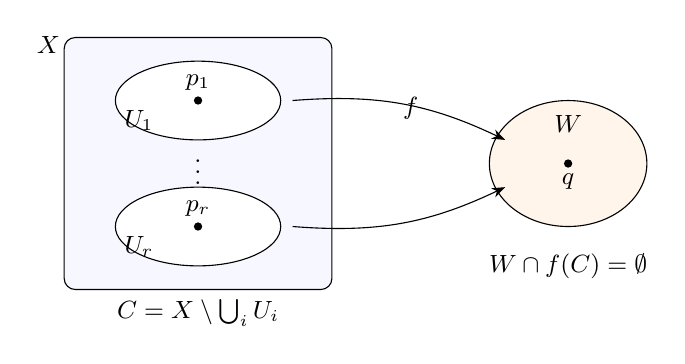
\begin{tikzpicture}[>=Stealth,every node/.style={font=\small}]
\draw[rounded corners,fill=blue!3] (-3.4,-1.6) rectangle (0,1.6);
\node at (-3.6,1.5) {$X$};
\draw[fill=white] (-1.7,.8) ellipse (1.05 and .5);
\draw[fill=white] (-1.7,-.8) ellipse (1.05 and .5);
\fill (-1.7,.8) circle (1.5pt) node[above] {$p_1$};
\fill (-1.7,-.8) circle (1.5pt) node[above] {$p_r$};
\node at (-2.45,.55) {$U_1$};
\node at (-2.45,-1.05) {$U_r$};
\node at (-1.7,0) {$\vdots$};
\node at (-1.7,-1.9) {$C=X\setminus\bigcup_i U_i$};
\draw[fill=orange!8] (3,0) ellipse (1 and .8);
\fill (3,0) circle (1.5pt) node[below] {$q$};
\node at (3,.5) {$W$};
\draw[->] (-.5,.8) to[bend left=15] (2.2,.3);
\draw[->] (-.5,-.8) to[bend right=15] (2.2,-.3);
\node at (1,.7) {$f$};
\node at (3,-1.3) {$W\cap f(C)=\emptyset$};
\end{tikzpicture}
\end{center}
図では二つの近傍だけを描いた.
$W$ を $f(C)$ から離して選ぶことで, 逆像が $U_i$ の外に現れる可能性を除いている.

$q'\in W\setminus\{q\}$ を取る.
$U_i$ 内で $f(p)=q'$ を解くことは
\[
t_i(p)^{e_i}=s_i(q')
\]
を解くことに等しい.
右辺は非零なので, 解は $U_i$ 内にちょうど $e_i$ 個あり, 
いずれも分岐指数は $1$ である.
$U_i$ の外に逆像はないから, 
\[
d(q')=\sum_i e_i=d(q)
\]
となる.よって $d$ は局所定値であり, $Y$ の連結性から一定である.

(2) 各 $e_p$ は $1$ 以上であり, $p$ が分岐点のときに限り $e_p>1$ である.
従って, 逆像に分岐点がなければ点の個数は $\deg f$ に等しく, 
分岐点があればそれより少ない.
また, $R$ は有限集合なので $f(R)$ も有限集合である.
\end{proof}


\begin{exa}[分岐指数とファイバーの点の個数]
正則写像
\[
f:\C\mathbb P^1\longrightarrow\C\mathbb P^1,\qquad
[s:t]\longmapsto[s^5-5st^4:t^5]
\]
を考える.
有限部分では $z=s/t$ として $f(z)=z^5-5z$ と表示される.
まず, 系\ref{cor-ramification-order}を使って分岐指数を求める.

\medskip
\noindent
\textbf{(1) 有限の点の場合.}

有限の点 $a$ での分岐指数は,
$f(z)-f(a)$ の $z=a$ における零点の位数である.
\[
f'(z)=5(z^4-1)
\]
なので, $a\notin\{1,-1,i,-i\}$ では $f'(a)\neq0$ であり,
分岐指数は $1$ である.

一方, $a\in\{1,-1,i,-i\}$ では,
$f'(a)=0$, $f''(a)=20a^3\neq0$ なので,
\[
f(z)-f(a)
=\underbrace{10a^3}_{\neq0}(z-a)^2+\cdots.
\]
従って, この四点での分岐指数は $2$ である.
また, $a^4=1$ より $f(a)=a^5-5a=-4a$ となる.

\medskip
\noindent
\textbf{(2) 無限遠点の場合.}

$f(\infty)=\infty$ なので,
始域では $w=1/z$, 終域では逆数の座標を使う.
このとき,
\[
\frac1{f(1/w)}
=\frac{w^5}{1-5w^4}
=w^5\underbrace{\frac1{1-5w^4}}_{w=0\text{ で非零}}
\]
となる.
零点の位数は $5$ なので, 無限遠点での分岐指数は $5$ である.

以上より, 分岐点と分岐値は次のとおりである.
\[
\begin{array}{c|ccccc}
\text{分岐点 }p&1&-1&i&-i&\infty\\ \hline
\text{分岐値 }f(p)&-4&4&-4i&4i&\infty\\
e_p&2&2&2&2&5
\end{array}
\]
また, $\infty$ の逆像は $\infty$ 一点だけなので,
\[
\deg f
\underalign{\text{(定理\ref{O-M071})}}{=}
\sum_{p\in f^{-1}(\infty)}e_p
=e_\infty=5.
\]

\medskip
\noindent
\textbf{(3) 各ファイバーの点を数える.}

定理\ref{O-M071}より, 任意の $q\in\C\mathbb P^1$ に対して
\[
\sum_{p\in f^{-1}(q)}e_p=5
\]
である.
従って, 各ファイバーの点の個数は,
分岐指数を使って次のように求められる.
\[
\begin{array}{c|c|c}
q&\displaystyle\sum_{p\in f^{-1}(q)}e_p&\#f^{-1}(q)\\ \hline
q\notin\{-4,4,-4i,4i,\infty\}
&1+1+1+1+1=5&5\\[2pt]
q\in\{-4,4,-4i,4i\}
&2+1+1+1=5&4\\[2pt]
q=\infty&5&1
\end{array}
\]
二行目では, 四つの有限の分岐点の像が互いに異なるため,
各ファイバーに分岐指数 $2$ の点が一つだけ含まれることを使った.

例えば, $q=-4$ では,
\[
f(z)+4=(z-1)^2(z^3+2z^2+3z+4).
\]
従って, 逆像は $z=1$ と三次式の相異なる三つの根からなる.
点の個数は $4$ だが, $z=1$ を重複度 $2$ で数えると $5$ になる.

このように, 逆像の点の個数は $q$ によって変わるが,
分岐指数を重複度として数えた個数は常に $\deg f=5$ である.
\end{exa}


% SOURCE O:2130 | O-M074 cor 2.29; original option: 2.29
\begin{cor}\label{O-M074}
コンパクトRiemann 面 $X$ からコンパクトRiemann 面 $Y$ への次数 $1$ の正則写像 $f$ は双正則写像である.
\end{cor}

\begin{proof}
次数が $1$ なので, 各ファイバーは分岐指数 $1$ の点1つからなり, 
$f$ は全単射である.

任意の $p\in X$ に対し, $q=f(p)$ とおく.
$p$ での分岐指数が $1$ なので, 局所標準形より, 
$p,q$ の座標近傍 $(\varphi,U),(\psi,V)$ を
\[
\psi\circ f\circ\varphi^{-1}(\zeta)=\zeta
\]
となるように取れる.従って
\[
f|_U=\psi^{-1}\circ\varphi,\qquad
(f|_U)^{-1}=\varphi^{-1}\circ\psi
\]
であり, 逆写像も正則である.
この局所逆写像は $f^{-1}|_V$ に等しいので, 
$f^{-1}$ は各点で正則であり, $f$ は双正則である.
\end{proof}

\subsection{コンパクトRiemann 面上の有理型関数の位数の総和}
% SOURCE O:2138 | O-M075 cor 2.30; original option: 2.30
\begin{cor}\label{O-M075}
$f$ をコンパクトRiemann 面 $X$ 上の $0$ ではない有理型関数とする. このとき
\[
\sum_{p\in X}\operatorname{ord}_p(f)=0
\]
である.
\end{cor}
ここで $\operatorname{ord}_p(f)$ は定義 \ref{O-M056} の符号付きの位数であり,
零点では正, 極では負である.
\begin{proof}
$f$ が非零定数ならば, すべての点で位数が $0$ なので明らかである.
以下, $f$ は定数でないとする.
定理\ref{O-M057}より, 極での値を $\infty$ と定めると,
正則写像 $\widetilde f:X\to\C\mathbb P^1$ が得られる.

零点と極では, その位数が $\widetilde f$ の分岐指数に等しい.
実際, $p$ を中心とする座標 $t$ で,
$m$ 位の零点ならば $f=t^m u(t)$,
$m$ 位の極ならば $f=t^{-m}u(t)$ と書ける.
ここで $u$ は正則で $u(0)\neq0$ である.
従って,
\[
\begin{array}{c|c|c}
p&\widetilde f\text{ の座標表示}&e_p\\ \hline
m\text{ 位の零点}&t^m u(t)&m\\[2pt]
m\text{ 位の極}&1/f=t^m/u(t)&m
\end{array}
\]
となる.
最後の列では, 座標表示の零点の位数が分岐指数であることを用いた
（系\ref{cor-ramification-order}参照）.

零点は $\widetilde f^{-1}(0)$, 極は $\widetilde f^{-1}(\infty)$ なので,
\[
\begin{aligned}
\sum_{p\in X}\operatorname{ord}_p(f)
&=
\underbrace{\sum_{p\in\widetilde f^{-1}(0)}e_p}_{\text{零点の位数の和}}
-
\underbrace{\sum_{p\in\widetilde f^{-1}(\infty)}e_p}_{\text{極の位数の和}}
\underalign{\text{(定理\ref{O-M071})}}{=}
\deg\widetilde f-\deg\widetilde f=0.
\end{aligned}
\]
よって, 結論を得る.
\end{proof}

\newpage

% SOURCE O:2178 | O-S017 Riemann 面上の微分形式
\section{Riemann 面上の微分形式}\label{O-S017}
接ベクトル空間や微分形式など多様体に関する物事に関しては, 定義を理解することと, 使えるようになることは全く別だと考えている. なので定義を完璧に理解できなくてもある程度良いと思う. 

\subsection{雑な微分形式の定義}

第\ref{O-S017}章の内容を, de Rhamコホモロジーを除いて概説する.
貼り合わせの説明までは $\C$ 上で考え,
接空間や位数を調べる点は $p=0$ とする.
以下, $z=x+iy$ とし, 関数は特に断らない限り
滑らかな複素数値関数とする.

\medskip
\noindent
$\bullet$ \textbf{微分の記号と接空間.}

まず $dx,dy$ を独立な記号として扱い,
複素座標に合わせて次の記号を使う
（\ref{O-S018}節, \ref{sec-holomorphic-tangent}節参照）.

\begin{dfn}[複素座標による微分の記号]
\[
dz:=dx+i\,dy,\qquad d\overline z:=dx-i\,dy,
\]
\[
\frac{\partial}{\partial z}
:=\frac12\left(
\frac{\partial}{\partial x}-i\frac{\partial}{\partial y}
\right),
\qquad
\frac{\partial}{\partial\overline z}
:=\frac12\left(
\frac{\partial}{\partial x}+i\frac{\partial}{\partial y}
\right)
\]
と定める.
原点での各空間は, 次の基底をもつ複素線形空間として考える.
\[
\begin{array}{c|c|c|c}
\text{名称}&\text{空間}&\text{基底}&\text{複素次元}\\ \hline
\text{複素接ベクトル空間}
&T_0^\C\C
&\left(\dfrac{\partial}{\partial z}\right)_0,
 \left(\dfrac{\partial}{\partial\overline z}\right)_0
&2\\[6pt]
\text{複素余接ベクトル空間}
&(T_0^\C\C)^*
&(dz)_0,(d\overline z)_0
&2\\[2pt]
\text{正則接ベクトル空間}
&T_0\C
&\left(\dfrac{\partial}{\partial z}\right)_0
&1\\[6pt]
\text{正則余接ベクトル空間}
&T_0^*\C
&(dz)_0
&1
\end{array}
\]
二行目は一行目の双対基底である.
最後の行では $(dz)_0$ を $T_0\C$ に制限して考える.
\end{dfn}

\medskip
\noindent
$\bullet$ \textbf{微分 $1$ 形式とその種類.}

余接ベクトルの係数を定数から関数に替えると, 微分形式になる
（\ref{O-S019}節, \ref{sec-meromorphic-one-forms}節参照）.

\begin{dfn}[微分 $1$ 形式]
$U\subset\C$ を開集合とする.
滑らかな関数を係数とする式
\[
\omega=a\,dx+b\,dy=A\,dz+B\,d\overline z
\]
を滑らかな微分 $1$ 形式といい, その全体を $A_\C^1(U)$ と書く.
各種類の形式全体を, 次の記号で表す.
\[
\begin{array}{c|c|c}
\text{形と係数の条件}&\text{名称}&\text{全体の記号}\\ \hline
A\,dz,\quad A\text{ は滑らか}
&(1,0)\text{ 形式}&A_{\C}^{1,0}(U)\\
B\,d\overline z,\quad B\text{ は滑らか}
&(0,1)\text{ 形式}&A_{\C}^{0,1}(U)\\
A\,dz,\quad A\text{ は正則}
&\text{正則 }1\text{ 形式}&\Omega_{\C}^1(U)\\
A\,dz,\quad A\text{ は有理型}
&\text{有理型 }1\text{ 形式}&\mathcal M_{\C}^1(U)
\end{array}
\]
ここでは, 有理型 $1$ 形式全体を $\mathcal M_\C^1(U)$ と書いた.
これらは開集合 $U$ 上の形式全体の空間であり,
一点での正則余接空間 $T_p^*\C$ とは区別する.

$dz,d\overline z$ は独立なので, 任意の滑らかな $1$ 形式は
\[
\omega
=\underbrace{A\,dz}_{(1,0)\text{ 形式}}
+\underbrace{B\,d\overline z}_{(0,1)\text{ 形式}}
\]
と一意に分解できる.
すなわち,
\[
A_\C^1(U)=A_\C^{1,0}(U)\oplus A_\C^{0,1}(U)
\]
である.

また, $0\in U$ のとき, 零でない有理型 $1$ 形式の原点での位数を
\[
\operatorname{ord}_0(A\,dz):=\operatorname{ord}_0(A)
\]
と定める.
\end{dfn}


例えば, $z^2\,dz$ は原点で二位の零点をもち,
$dz/z$ は原点で一位の極をもつ.
$\overline z\,dz$ は滑らかな $(1,0)$ 形式だが,
正則 $1$ 形式ではない.

\medskip
\noindent
$\bullet$ \textbf{外積と微分 $2$ 形式.}
（\ref{O-S020}節参照）

\begin{dfn}[外積と微分 $2$ 形式]
$U\subset\C$ を開集合とする.
外積 $\wedge$ は, 分配法則と
\[
dx\wedge dx=dy\wedge dy=0,\qquad
dy\wedge dx=-dx\wedge dy
\]
に従う積である.

滑らかな関数 $c$ を係数とする式
\[
\eta=c\,dx\wedge dy
\]
を滑らかな微分 $2$ 形式といい,
その全体を $A_\C^2(U)$ と書く.

$dz\wedge d\overline z=-2i\,dx\wedge dy$ なので,
$\eta$ は一意に $C\,dz\wedge d\overline z$ とも書ける.
この形の形式を $(1,1)$ 形式といい,
その全体を $A_\C^{1,1}(U)$ と書く.
従って,
\[
A_\C^2(U)=A_\C^{1,1}(U)
\]
である.
\end{dfn}
例えば,
\[
(a\,dx+b\,dy)\wedge(c\,dx+d\,dy)
=(ad-bc)\,dx\wedge dy.
\]
また, $dz\wedge d\overline z=-2i\,dx\wedge dy$ なので,
$2$ 形式は $C\,dz\wedge d\overline z$ とも書ける.
これを $(1,1)$ 形式という.

\medskip
\noindent
$\bullet$ \textbf{外微分は係数を微分する操作.}
（\ref{sec-differential-functions}節, \ref{O-S021}節参照）

\begin{dfn}[外微分]
関数を $0$ 形式と呼び, その外微分を
\[
df:=\frac{\partial f}{\partial x}\,dx
+\frac{\partial f}{\partial y}\,dy
=\frac{\partial f}{\partial z}\,dz
+\frac{\partial f}{\partial\overline z}\,d\overline z
\]
と定める.
$1$ 形式の外微分は
\[
d(a\,dx+b\,dy)
:=\left(
\frac{\partial b}{\partial x}-\frac{\partial a}{\partial y}
\right)dx\wedge dy
\]
と定め, $2$ 形式の外微分は零とする.
\end{dfn}

例えば, $d(z^2)=2z\,dz$, $d(x\,dy)=dx\wedge dy$ である.
複素座標では
\[
d(A\,dz+B\,d\overline z)
=\left(
\frac{\partial B}{\partial z}
-\frac{\partial A}{\partial\overline z}
\right)dz\wedge d\overline z
\]
なので, 正則 $1$ 形式の外微分は零である.
また, 混合偏微分の順序を交換できることから $d(df)=0$ となる.

\medskip
\noindent
$\bullet$ \textbf{引き戻しは代入する操作.}
（\ref{O-S022}節参照）

\begin{dfn}[引き戻し]
正則写像 $f:\C\to\C$, $w=F(z)$ に対し,
終域の形式に
\[
w=F(z),\qquad
dw=\frac{dF}{dz}(z)\,dz,\qquad
d\overline w=\overline{\frac{dF}{dz}(z)}\,d\overline z
\]
を代入したものを引き戻し $f^*\omega$ という.
\end{dfn}

例えば, $F(z)=z^2$ ならば,
\[
f^*(w\,dw)=2z^3\,dz,\qquad
f^*\left(\frac{dw}{w}\right)=2\frac{dz}{z}.
\]
また, $F(z)=z^e$, $\omega=w^m u(w)\,dw$, $u(0)\neq0$ ならば,
\[
f^*\omega=e\,u(z^e)z^{em+e-1}dz.
\]
この位数 $em+e-1$ が分岐公式のもとになる
（\ref{O-S023}節参照）.

\medskip
\noindent
$\bullet$ \textbf{積分は線積分と面積分.}
（\ref{O-S024}節参照）

\begin{dfn}[微分形式の積分]
曲線 $\gamma(t)=(x(t),y(t))$, $t_0\leq t\leq t_1$ に対して,
\[
\int_\gamma(a\,dx+b\,dy)
:=\int_{t_0}^{t_1}
\left(
a(\gamma(t))\frac{dx}{dt}(t)
+b(\gamma(t))\frac{dy}{dt}(t)
\right)dt
\]
と定める.
また, 平面内の領域 $D$ 上では,
\[
\int_D c\,dx\wedge dy:=\iint_D c(x,y)\,dx\,dy
\]
と定める.
ここでは標準の向きを使い, 積分は収束する場合に考える.
\end{dfn}

つまり, 線積分では
$dx=\frac{dx}{dt}(t)\,dt$,
$dy=\frac{dy}{dt}(t)\,dt$ を代入し,
$2$ 形式の積分では通常の面積分を計算すればよい.

\medskip
\noindent
$\bullet$ \textbf{局所座標で書き, 重なりで貼り合わせる.}

ここから一般のRiemann 面 $X$ を考える.
各局所座標では上の計算をそのまま使い,
\textbf{重なりで一致する局所表示を貼り合わせる}
（\ref{O-S019}節, \ref{O-S020}節参照）.

\begin{dfn}[Riemann 面上の微分形式]
Riemann 面では, 場所ごとに局所座標を選び,
その座標で微分形式を書く.
例えば, $z$ 座標では $A(z)\,dz$,
$w$ 座標では $B(w)\,dw$ と書く.

二つの座標が使えるところで,
\[
dw=\frac{dw}{dz}\,dz
\]
を代入して同じ式になれば,
これらを\textbf{同じ微分形式の別の座標表示}と考える.
このように, 各場所での式をつなぎ合わせたものが,
Riemann 面上の微分形式である.
これを微分形式の貼り合わせという.
\end{dfn}

\begin{exa}
後の例\ref{O-M094}で扱う,
$\C\mathbb P^1$ 上の有理型 $1$ 形式を考える.
有限部分での式を $dz$ とすると,
無限遠点の座標 $w=1/z$ では,
\[
dz=d(1/w)=-\frac1{w^2}\,dw
\]
となる.
従って,
\[
\begin{array}{c|c}
\text{使う座標}&\text{同じ形式の表示}\\ \hline
z&dz\\[2pt]
w&-\dfrac1{w^2}\,dw
\end{array}
\]
という二つの式で, 球面全体の一つの有理型 $1$ 形式を表せる.
有限部分では係数が $1$ なので零点も極もなく,
無限遠点 $w=0$ では係数 $-1/w^2$ が二位の極をもつ.
\end{exa}

\begin{exa}[球面上の滑らかな $1$ 形式]
後の例\ref{exa-sphere-smooth-one-form}では,
次の二つの式を貼り合わせる：
\[
\eta_z=\frac{\overline z}{(1+|z|^2)^2}\,dz,
\qquad
\eta_w=-\frac{\overline w}{(1+|w|^2)^2}\,dw.
\]
実際, $z=1/w$ を代入すると,
\[
\eta_z
=\frac{1/\overline w}{(1+1/|w|^2)^2}
\left(-\frac1{w^2}\,dw\right)
=-\frac{\overline w}{(1+|w|^2)^2}\,dw
=\eta_w.
\]
従って, 二つの式は球面全体の一つの滑らかな $1$ 形式を表す.
ただし, 係数は正則ではないので, 正則 $1$ 形式ではない.
\end{exa}

\begin{exa}[球面上の滑らかな $2$ 形式]
$2$ 形式も, 同じ座標に直して一致すれば貼り合わせられる.
後の例\ref{exa-sphere-two-form}では,
\[
\sigma_z=\frac{i}{2}\frac{dz\wedge d\overline z}{(1+|z|^2)^2},
\qquad
\sigma_w=\frac{i}{2}\frac{dw\wedge d\overline w}{(1+|w|^2)^2}
\]
を考える.
$z=1/w$ とすると,
\[
dz\wedge d\overline z
=\frac1{|w|^4}\,dw\wedge d\overline w,
\qquad
(1+|z|^2)^2=\frac{(1+|w|^2)^2}{|w|^4}.
\]
分子と分母に同じ因子が現れるので,
$\sigma_z=\sigma_w$ となる.
従って, これらは球面全体の滑らかな $2$ 形式を定める.

$z=x+iy$ で書けば
\[
\sigma_z=\frac1{(1+x^2+y^2)^2}\,dx\wedge dy
\]
となり, 平面の面積要素に重みを付けたものと考えられる.
\end{exa}


% SOURCE O:2184 | O-S018 複素接空間と余接ベクトル空間
\subsection{複素接ベクトル空間と複素余接ベクトル空間}\label{O-S018}

まず厳密な定義を書いてから, ラフな定義を述べる. 
\begin{dfn}[$C^\infty$ 級関数の芽]\label{dfn-smooth-germ}
$p\in X$ とする.
$p$ の開近傍上の複素数値 $C^\infty$ 級関数の対 $(f,U)$ に対し, 
\[
(f,U)\sim(g,V)
\iff
p\text{ のある開近傍 }W\subset U\cap V\text{ 上で }f=g
\]
と定める.
この同値関係による同値類を $p$ における $C^\infty$ 級関数の芽といい, 
$f$ の定める芽を $[f]$, 芽全体を $A^0_{X,p}$ と書く.
$A^0_{X,p}$ は
\[
[f]+[g]=[f+g],\qquad [f][g]=[fg],\qquad c[f]=[cf]\quad(c\in\C)
\]
により $\C$-代数となる.ただし, 演算は共通の近傍上で行う.
\end{dfn}

\begin{dfn}[$\C$-代数]
単位元をもつ可換環 $A$ と, 単位元を保つ環準同型
\(
\iota:\C\longrightarrow A
\)
の組で, 任意の $c\in\C$ と $a\in A$ に対して
\(
\iota(c)a=a\iota(c)
\)
が成り立つものを $\C$-代数という.
\end{dfn}

% SOURCE O:2188 | O-M078 defn 3.1; original option: 3.1
\begin{dfn}[複素接空間]\label{O-M078}
$p\in X$ とし, $A^0_{X,p}$ を $p$ における複素数値 $C^\infty$ 級関数の芽の代数とする.
$\C$-線形写像 $v:A^0_{X,p}\to\C$ が
\[
v(fg)=f(p)v(g)+g(p)v(f)
\]
を満たすとき, $v$ を $p$ における複素接ベクトルという.
その全体
\[
T_p^{\C}X
:=
\{v:A^0_{X,p}\to\C\mid v\text{ は }\C\text{-線形で上の積の法則を満たす}\}
\]
を複素接空間という.
関数の芽の値 $f(p)$ は代表元の選び方によらない.
\end{dfn}
\begin{rem}
実接空間を $T_p^{\mathbb R}X$ と書けば,
$T_p^\C X\simeq T_p^{\mathbb R}X\otimes_{\mathbb R}\C$ である.
これは実 $2$ 次元の接空間を複素係数に拡張した空間であり,
後で定義する複素 $1$ 次元の正則接空間 $T_pX$ とは区別する.
\end{rem}

\begin{rem}
$v$ を $T_{p}^{\C}X$ の元とする. $v([1])=v([1][1])=1v([1])+1v([1])$ より $v([1])=0$ である. 従って, 定数関数 $a$ に対しても $v([a])=v(a[1])=av([1])=0$ である.
\end{rem}

\begin{ex}
$(\varphi,V)$ を $p$ の属する座標近傍系とする. $z$ を実部と虚部に分けて,
\[
z=x+\sqrt{-1}y
\]
と書く. $\varphi(p)=a+ib$ とおく. $p$ の近傍で定義された $C^\infty$ 級関数は実座標 $(x,y)$ を用いて $f(x,y)$ の形に座標表示される. $f(x,y)$ は $(a,b)$ の近傍で $C^\infty$ 級である. $p$ での偏微分
\[
\left(\frac{\partial}{\partial x}\right)_p;\ f\longmapsto \frac{\partial f}{\partial x}(a,b),\quad
\left(\frac{\partial}{\partial y}\right)_p;\ f\longmapsto \frac{\partial f}{\partial y}(a,b)
\]
は $T_{p}^{\C}X$ の元を定める. 点 $p$ での偏微分は, 局所的に定まる操作であり, しかも定義 \ref{O-M078} にある線形性とLeibniz則をみたすからである. 以下, 点 $p$ とその実座標値 $(a,b)$ を同一視する.
\end{ex}

% SOURCE O:2219 | O-M079 lem 3.2; original option: 3.2
\begin{lem}\label{O-M079}
$T_{p}^{\C}X$ は
\[
\left(\left(\frac{\partial}{\partial x}\right)_p,\left(\frac{\partial}{\partial y}\right)_p\right)
\]
を基底とする $2$ 次元 $\C{}$-線形空間である.
\end{lem}
\begin{proof}
$v\in T_{p}^{\C}X$ とする.
Taylorの定理より, $p=(a,b)$ の近くで
\[
f=f(p)+(x-a)F+(y-b)G,
\qquad F(p)=\frac{\partial f}{\partial x}(p),\quad G(p)=\frac{\partial f}{\partial y}(p)
\]
と書ける.ただし $F,G$ は $C^\infty$ 級関数である.
$v$ は定数を $0$ に写すので, Leibniz則から
\[
v([f])=v([x])\frac{\partial f}{\partial x}(p)+v([y])\frac{\partial f}{\partial y}(p)
\]
を得る.従って
\[
v=v([x])\left(\frac{\partial}{\partial x}\right)_p
 +v([y])\left(\frac{\partial}{\partial y}\right)_p
\]
であり, 2つの偏微分作用素は $T_{p}^{\C}X$ を生成する.
また, これらの線形結合を $[x],[y]$ に作用させれば, 
係数がそれぞれ取り出せるので, 一次独立でもある.
\end{proof}





% SOURCE O:2264 | O-M081 defn 3.3; original option: 3.3
\begin{dfn}\label{O-M081}
$T_{p}^{\C}X$ の双対空間
\[
(T_{p}^{\C}X)^*:=\OSourceHom_{\C{}}(T_{p}^{\C}X,\C{})
\]
のことを $p$ における $X$ の余接ベクトル空間という.

つまり
$\langle (dx)_p,(dy)_p\rangle$ を $T_{p}^{\C}X$ の基底
\(
\left\langle \left(\frac{\partial}{\partial x}\right)_p,\left(\frac{\partial}{\partial y}\right)_p\right\rangle
\)
の双対基底とするとき, $(dx)_p,(dy)_p$ はそれぞれ
\[
\begin{aligned}
(dx)_p\left(\frac{\partial}{\partial x}\Big|_p\right)&=1,
&\qquad
(dx)_p\left(\frac{\partial}{\partial y}\Big|_p\right)&=0,\\
(dy)_p\left(\frac{\partial}{\partial x}\Big|_p\right)&=0,
&\qquad
(dy)_p\left(\frac{\partial}{\partial y}\Big|_p\right)&=1.
\end{aligned}
\]
によって一意に定まる $(T_{p}^{\C}X)^*$ の元であり, $\langle (dx)_p,(dy)_p\rangle$ は $(T_{p}^{\C}X)^*$ の基底をなす.
\end{dfn}

$u$ を $(T_{p}^{\C}X)^*$ の元とする. このとき, 次の等式が成り立つ：
\[
u=
u\left(\left(\frac{\partial}{\partial x}\right)_p\right)(dx)_p+
u\left(\left(\frac{\partial}{\partial y}\right)_p\right)(dy)_p.
\]
実際, $T_{p}^{\C}X$ の基底
\[
\left\langle \left(\frac{\partial}{\partial x}\right)_p,\left(\frac{\partial}{\partial y}\right)_p\right\rangle
\]
の像が左辺と右辺で一致するからである.


とここまで定義したが, やっぱり$T_{p}^{\C}X$の定義はかなり難しい!　そして定義通りに計算することはあんまりない(と思う). 
なのでわからない人は次のように思って良い. 
\begin{tcolorbox}[mybox]

\begin{itemize}
\item 複素接空間$T_{p}^{\C}X$ は, 
\(
\left(\frac{\partial}{\partial x}\right)_p,
\left(\frac{\partial}{\partial y}\right)_p
\)
を基底とする $2$ 次元 $\C$-線形空間. 
\item  複素余接空間$(T_{p}^{\C}X)^*$ は, 
双対基底
\(
(dx)_p, (dy)_p
\)
をもつ $2$ 次元 $\C$-線形空間
\end{itemize}
なお
$
\left(\frac{\partial}{\partial x}\right)_p,
\left(\frac{\partial}{\partial y}\right)_p. 
(dx)_p, (dy)_p$の意味は考えない. 
\end{tcolorbox}

\subsection{外微分}\label{sec-differential-functions}

% SOURCE O:2317 | O-M083 defn 3.4; original option: 3.4
\begin{dfn}\label{O-M083}
$f$ を $p$ の近傍で定義された $C^\infty$ 級関数とする. $f$ は写像
\[
(df)_p : T_{p}^{\C}X\to \C{};\quad v\longmapsto v([f])
\]
を定める. この写像のことを $(df)_p$ と書き, $f$ の $p$ における外微分または全微分という.
$(df)_p\in (T_{p}^{\C}X)^*$ である.
\end{dfn}

% SOURCE O:2327 | O-M084 lem 3.5; original option: 3.5
\begin{lem}\label{O-M084}
$f$ は定義 \ref{O-M083} の通りとする. このとき次の等式が成立する：
\[
(df)_p=\frac{\partial f}{\partial x}(p)(dx)_p+\frac{\partial f}{\partial y}(p)(dy)_p.
\]
\end{lem}

\begin{proof}
定義から,
\[
(df)_p\left(\left(\frac{\partial}{\partial x}\right)_p\right)=\frac{\partial f}{\partial x}(p),\quad
(df)_p\left(\left(\frac{\partial}{\partial y}\right)_p\right)=\frac{\partial f}{\partial y}(p)
\]
\end{proof}

\begin{exa}[接ベクトルと全微分の計算]
$X=\C$, $z=x+iy$ とし, $p=1$, すなわち $(x,y)=(1,0)$ とする.
接ベクトル
\[
v=2\left(\frac{\partial}{\partial x}\right)_p
 +3\left(\frac{\partial}{\partial y}\right)_p
\]
は, 関数の芽 $[f]$ に対して
\[
v([f])=2\frac{\partial f}{\partial x}(1,0)+3\frac{\partial f}{\partial y}(1,0)
\]
を対応させる微分作用素である.
一方, 余接ベクトル $(dx)_p,(dy)_p$ は, この係数を取り出す：
\[
(dx)_p(v)=2,\qquad (dy)_p(v)=3.
\]

例えば $f(x,y)=x^2+xy$ ならば, 
$\frac{\partial f}{\partial x}(p)=2$, $\frac{\partial f}{\partial y}(p)=1$ なので, 
\[
(df)_p=2(dx)_p+(dy)_p.
\]
従って
\[
(df)_p(v)=2\cdot2+1\cdot3=7=v([f])
\]
となり, 全微分の定義が具体的に確認できる.
\end{exa}

\subsection{正則接ベクトル空間}\label{sec-holomorphic-tangent}

座標 $z=x+iy$ とその複素共役 $\overline z=x-iy$ に
補題 \ref{O-M084} を適用すると, 
\[
(dz)_p=(dx)_p+i(dy)_p,\qquad
(d\overline z)_p=(dx)_p-i(dy)_p
\]
を得る.また, 次の微分作用素を定める：
\[
\begin{aligned}
\left(\frac{\partial}{\partial z}\right)_p
&:=\frac12\left(
\left(\frac{\partial}{\partial x}\right)_p
-i\left(\frac{\partial}{\partial y}\right)_p\right),
\qquad
\left(\frac{\partial}{\partial\overline z}\right)_p
&:=\frac12\left(
\left(\frac{\partial}{\partial x}\right)_p
+i\left(\frac{\partial}{\partial y}\right)_p\right).
\end{aligned}
\]

\begin{cor}\label{O-M085}
$(dz)_p,(d\overline z)_p$ は $(T_{p}^{\C}X)^*$ の基底であり, 
\(
\left(\frac{\partial}{\partial z}\right)_p,
\left(\frac{\partial}{\partial\overline z}\right)_p
\)
は, それに対応する $T_{p}^{\C}X$ の双対基底である.
\end{cor}

\begin{proof}
定義から, 
\[
\begin{aligned}
(dz)_p\left(\frac{\partial}{\partial z}\Big|_p\right)&=1,
&
(dz)_p\left(\frac{\partial}{\partial\overline z}\Big|_p\right)&=0,\\
(d\overline z)_p\left(\frac{\partial}{\partial z}\Big|_p\right)&=0,
&
(d\overline z)_p\left(\frac{\partial}{\partial\overline z}\Big|_p\right)&=1
\end{aligned}
\]
となるので, 両者は互いに双対な基底である.
\end{proof}

\begin{lem}[座標変換と $dz,d\overline z$]\label{O-M086}
$p$ を含む二つの座標近傍 $(\varphi,V),(\psi,W)$ を取り,
座標変数をそれぞれ $z,w$ とする.
座標変換 $w=F(z)$, $F=\psi\circ\varphi^{-1}$ に対して,
\[
(dw)_p=\frac{dF}{dz}(\varphi(p))(dz)_p,\qquad
(d\overline w)_p=
\overline{\frac{dF}{dz}(\varphi(p))}(d\overline z)_p
\]
が成り立つ.
ここで $\dfrac{dF}{dz}(\varphi(p))\neq0$ である.

従って, $(dz)_p$ が張る部分空間と
$(d\overline z)_p$ が張る部分空間は,
それぞれ座標の選び方によらない.
\end{lem}

\begin{proof}
$z=x+iy$ とする.
$F$ は正則なので, Cauchy--Riemannの関係式から
\[
\frac{\partial F}{\partial x}=\frac{dF}{dz},
\qquad
\frac{\partial F}{\partial y}
\underalign{\text{(定理\ref{thm-cauchy-riemann})}}{=}
i\frac{dF}{dz}
\]
である.
従って, 座標関数 $w=F(z)$ の全微分は
\[
\begin{aligned}
(dw)_p
&\underalign{\text{(補題\ref{O-M084})}}{=}
\frac{\partial F}{\partial x}(\varphi(p))(dx)_p
+\frac{\partial F}{\partial y}(\varphi(p))(dy)_p
=\frac{dF}{dz}(\varphi(p))
\underbrace{\bigl((dx)_p+i(dy)_p\bigr)}_{=(dz)_p}
=\frac{dF}{dz}(\varphi(p))(dz)_p.
\end{aligned}
\]
この等式の複素共役を取れば,
$(d\overline w)_p$ の式も得られる.

また, $F$ は正則な逆写像をもつので, 連鎖律より
\[
\frac{dF^{-1}}{dw}(\psi(p))
\frac{dF}{dz}(\varphi(p))
=1.
\]
従って $\dfrac{dF}{dz}(\varphi(p))\neq0$ である.
つまり, 座標を変えても $(dz)_p$ と $(d\overline z)_p$ は
それぞれ非零の定数倍に変わるだけなので,
それぞれが張る部分空間は変わらない.
\end{proof}

\begin{thm}[Cauchy--Riemannの関係式]\label{thm-cauchy-riemann}
複素平面の開集合上の $C^1$ 級関数 $F=u+iv$ について,
\[
F\text{ が正則}
\quad\Longleftrightarrow\quad
\frac{\partial u}{\partial x}=\frac{\partial v}{\partial y},\quad \frac{\partial u}{\partial y}=-\frac{\partial v}{\partial x}
\quad\Longleftrightarrow\quad
\frac{\partial F}{\partial\bar z}
=\frac12(\frac{\partial F}{\partial x}+i\frac{\partial F}{\partial y})=0.
\]
このとき $F'(z)=\frac{\partial F}{\partial x}$ である.
\end{thm}

接ベクトルの基底は, 余接ベクトルの基底と双対なので, 
補題\ref{O-M086}の座標変換 $F=\psi\circ\varphi^{-1}$ に対して
\[
\left(\frac{\partial}{\partial w}\right)_p
=\frac{1}{\dfrac{dF}{dz}(\varphi(p))}\left(\frac{\partial}{\partial z}\right)_p,\qquad
\left(\frac{\partial}{\partial\overline w}\right)_p
=\frac{1}{\overline{\dfrac{dF}{dz}(\varphi(p))}}
 \left(\frac{\partial}{\partial\overline z}\right)_p
\]
となる.従って, こちらも各基底が生成する部分空間は座標によらない.

\begin{dfn}[正則接ベクトル空間]
$p\in X$ に対し, 
\[
T_pX:=\C\left(\frac{\partial}{\partial z}\right)_p
\]
を, $p$ における $X$ の正則接ベクトル空間という.
これは座標の選び方によらない, 複素1次元のベクトル空間である.

$T_pX$ の共役複素ベクトル空間を $\overline{T_pX}$ と書く.
接ベクトルの複素共役により, これを部分空間
\[
\overline{T_pX}=
\C\left(\frac{\partial}{\partial\overline z}\right)_p
\]
と同一視すると, 
\[
T_{p}^{\C}X=T_pX\oplus \overline{T_pX}
\]
となる.この分解は, $X$ の複素構造に依存する.
\end{dfn}

正則接ベクトル空間の双対空間を
\[
T_p^*X:=(T_pX)^*
\]
と書き, 正則余接ベクトル空間という.
$(dz)_p$ を $T_pX$ に制限することで,
$\C(dz)_p\subset(T_p^\C X)^*$ と $T_p^*X$ を自然に同一視する.
共役の空間についても同様に,
\[
T_p^*X=\C(dz)_p,\qquad
\overline{T_p^*X}=\C(d\overline z)_p,\qquad
(T_p^\C X)^*=T_p^*X\oplus\overline{T_p^*X}
\]
と表せる.これらの部分空間は座標の選び方によらない
（補題\ref{O-M086}参照）.

\begin{exa}[Riemann 球面での座標変換]
$X=\C\mathbb P^1$ とし, $p=[2:1]$ において
座標変換 $w=1/z$ を考える.
$\varphi_1(p)=2$, $\varphi_0(p)=1/2$ なので,
\[
\left.\frac{dw}{dz}\right|_{z=2}=-\frac14.
\]
従って
\[
(dw)_p=-\frac14(dz)_p,\qquad
\left.\frac{\partial}{\partial w}\right|_p
=-4\left.\frac{\partial}{\partial z}\right|_p.
\]
基底は変わるが, 互いに逆数倍されるため,
\[
(dw)_p\left(\frac{\partial}{\partial w}\Big|_p\right)=1
\]
という双対関係は保たれる.

また, 基底が非零定数倍されるだけなので, 
\[
\C(dz)_p=\C(dw)_p,\qquad
\C\left(\frac{\partial}{\partial z}\right)_p
=\C\left(\frac{\partial}{\partial w}\right)_p.
\]
従って, 正則接空間・正則余接空間は, 
$z,w$ のどちらで計算しても同じ部分空間になる.
\end{exa}


とここまで定義したが, やっぱり $T_pX$ の定義はかなり難しい!
なのでわからない人は次のように思って良い.
\begin{tcolorbox}[mybox]
座標 $z=x+iy$ について
\[
(dz)_p=(dx)_p+i(dy)_p,\qquad
(d\overline z)_p=(dx)_p-i(dy)_p
\]
\[
\begin{aligned}
\left(\frac{\partial}{\partial z}\right)_p
&:=\frac12\left(
\left(\frac{\partial}{\partial x}\right)_p
-i\left(\frac{\partial}{\partial y}\right)_p\right),
\qquad
\left(\frac{\partial}{\partial\overline z}\right)_p
&:=\frac12\left(
\left(\frac{\partial}{\partial x}\right)_p
+i\left(\frac{\partial}{\partial y}\right)_p\right).
\end{aligned}
\]
を意味を考えずに考える. 
\begin{itemize}
\item 複素接空間 $T_p^{\C}X$ は,
\(
\left(\frac{\partial}{\partial z}\right)_p,
\left(\frac{\partial}{\partial\overline z}\right)_p
\)
を基底とする $2$ 次元 $\C$-線形空間.

\item 複素余接空間 $(T_p^{\C}X)^*$ は,
双対基底
\(
(dz)_p,(d\overline z)_p
\)
をもつ $2$ 次元 $\C$-線形空間.

\item 正則接ベクトル空間 $T_pX$ は,
\(
\left(\frac{\partial}{\partial z}\right)_p
\)
で張られる $1$ 次元 $\C$-線形空間.
これは $T_p^{\C}X$ の部分空間である.

\item 正則余接ベクトル空間 $T_p^*X$ は,
\(
(dz)_p
\)
を基底とする $1$ 次元 $\C$-線形空間.
ここでは $(dz)_p$ を $T_pX$ に制限して考える.
\end{itemize}
まずは, これらを基底の記号として扱えばよい.
特に, 双対基底の関係は
\[
\begin{array}{c|cc}
 & \left(\dfrac{\partial}{\partial z}\right)_p
 & \left(\dfrac{\partial}{\partial\overline z}\right)_p\\ \hline
(dz)_p&1&0\\
(d\overline z)_p&0&1
\end{array}
\]
である.
\end{tcolorbox}

% SOURCE O:2493 | O-S019 微分 $1$ 形式
\subsection{微分 $1$ 形式・正則1形式}\label{O-S019}
まず厳密な定義をしてから, それからラフな定義を述べる. 以下$U\subset X$ を空でない開集合とし, $U$ 上の複素数値 $C^\infty$ 級関数全体を
$A_X^0(U)$, 正則関数全体を $\mathcal O_X(U)$ と書く.\footnote{この記号の意味は\ref{O-S032}章でわかるが今はそういうものだと思ってほしい}

\begin{dfn}[微分 $1$ 形式]
$X$ をRiemann 面, $U\subset X$ を開集合とする.
各点 $p\in U$ に, その点の余接ベクトル
\[
\eta_p\in(T_p^\C X)^*
\]
を一つずつ与えたものを, $U$ 上の微分 $1$ 形式という.
つまり, $\eta_p$ は $p$ での接ベクトルを受け取り,
複素数を返す線形写像である.

局所座標 $z$ をもつ座標近傍 $V\subset U$ では,
$(dz)_p,(d\overline z)_p$ が余接空間の基底なので,
\[
\eta_p=a(p)(dz)_p+b(p)(d\overline z)_p
\qquad(p\in V)
\]
と一意に書ける.
この式を各点についてまとめた表示
\[
\eta|_V=a\,dz+b\,d\overline z
\]
を, $\eta$ の座標表示という.
ここで $a,b$ は $V$ 上の複素数値関数である.
\end{dfn}

座標を変えると, 基底となる $1$ 形式は次のように変換される.

\begin{lem}[座標変換と $1$ 形式]\label{O-M088}
2つの座標近傍 $(\varphi,V),(\psi,W)$ の共通部分で, 次が成り立つ.
\begin{enumerate}
\item 複素座標では
\[
dw=\frac{dw}{dz}\,dz,\qquad
d\overline w=\overline{\frac{dw}{dz}}\,d\overline z.
\]
\item $z=x+iy$, $w=u+iv$ と実座標で表すと, 
\[
du=\frac{\partial u}{\partial x}\,dx
  +\frac{\partial u}{\partial y}\,dy,\qquad
dv=\frac{\partial v}{\partial x}\,dx
  +\frac{\partial v}{\partial y}\,dy.
\]
\end{enumerate}
\end{lem}

\begin{proof}
(1) は補題 \ref{O-M086}, (2) は全微分の公式を, 
$V\cap W$ の各点で適用したものである.
\end{proof}


\begin{exa}\label{O-M089}
同じ座標変換でも, 実座標で計算すると式が長くなり,
複素座標なら一つの式で書けることを確認する.
$\C\mathbb P^1=\C_z\cup\C_w$ とし, $z=x+iy$, $w=u+iv$ とおく.
共通部分では $w=1/z$ なので, 実座標による変換則は
\[
\begin{aligned}
du&=\frac{y^2-x^2}{(x^2+y^2)^2}\,dx
   -\frac{2xy}{(x^2+y^2)^2}\,dy,\\
dv&=\frac{2xy}{(x^2+y^2)^2}\,dx
   +\frac{y^2-x^2}{(x^2+y^2)^2}\,dy
\end{aligned}
\]
となる.一方, 複素座標では単に $dw=-z^{-2}dz$ と書ける.
\end{exa}

\begin{proof}
\[
w=\frac1z=\frac{x-iy}{x^2+y^2}
\]
の実部と虚部を比較すると, 
\[
u=\frac{x}{x^2+y^2},\qquad
v=-\frac{y}{x^2+y^2}
\]
を得る.これらを $x,y$ で偏微分し, 
$du=\frac{\partial u}{\partial x}\,dx+\frac{\partial u}{\partial y}\,dy$, $dv=\frac{\partial v}{\partial x}\,dx+\frac{\partial v}{\partial y}\,dy$ に代入すればよい.
\end{proof}


\begin{dfn}\label{O-M090}
$U\subset X$ を開集合とし, $U$ 上の $1$ 形式 $\eta$ を, 
各座標近傍で
\[
\eta=a\,dz+b\,d\overline z
\]
と表示する.
\begin{enumerate}
\item
係数 $a,b$ が $C^\infty$ 級であるとき, 
$\eta$ を $C^\infty$ 級 $1$ 形式という.
その全体を $A_X^1(U)$ と書く.

\item
$C^\infty$ 級 $1$ 形式のうち, 
\[
\eta=a\,dz
\]
と書けるものを $(1,0)$ 形式, 
\[
\eta=b\,d\overline z
\]
と書けるものを $(0,1)$ 形式という.
それぞれの全体を $A_X^{1,0}(U)$, $A_X^{0,1}(U)$ と書く.

\item
$\eta=a\,dz$ と書け, 係数 $a$ が正則であるとき, 
$\eta$ を正則 $1$ 形式という.その全体を $\Omega_X^1(U)$ と書く.
\end{enumerate}
これらの条件は, 座標変換則により座標の選び方によらない.
\end{dfn}

任意の $C^\infty$ 級 $1$ 形式は, 
$(1,0)$ 形式と $(0,1)$ 形式の和に一意に分解される：
\[
A_X^1(U)=A_X^{1,0}(U)\oplus A_X^{0,1}(U).
\]
これらは $C^\infty$ 級関数を掛けても同じ種類の形式となるので, 
$A_X^0(U)$-加群である.
また, $\Omega_X^1(U)$ は $\mathcal O_X(U)$-加群である.

\begin{rem}\label{O-M091}
$A_X^1(U)$ は下部 $C^\infty$ 級構造だけで定まるが, 
$(1,0)$ 型・$(0,1)$ 型への分解$A_X^{1,0}(U)$, $A_X^{0,1}(U)$と正則性$\Omega_X^1(U)$ は, 
$X$ の複素構造に依存する.
\end{rem}

以上が厳密な定義であるが, 少々使いづらいしわかりづらく私は好きではない. 
以下のような別の定義も述べる\footnote{これはベクトル束のsectionという観点からみた定義である.}
なお定義としては同じであるので理解しやすい方で理解してほしい. 

\begin{prop}[$1$ 形式の貼りあわせ]\label{prop-gluing-one-forms}
$U=\bigcup_i U_i$ を座標近傍 $(\varphi_i,U_i)$ による開被覆とし, 
各 $U_i$ 上に $1$ 形式
\[
\eta_i=a_i\,dz_i+b_i\,d\overline z_i
\]
が与えられているとする.
共通部分 $U_i\cap U_j$ で, 同じ座標を使って表示したときに
$\eta_i=\eta_j$ となるならば, 
これらは $U$ 上の一意な $1$ 形式 $\eta$ に貼りあわされる.

具体的には, $z_j$ 座標に直すと
\[
\eta_i
=a_i\frac{dz_i}{dz_j}\,dz_j
+b_i\overline{\frac{dz_i}{dz_j}}\,d\overline z_j
\]
なので, 貼りあわせの条件は
\[
a_j=a_i\frac{dz_i}{dz_j},\qquad
b_j=b_i\overline{\frac{dz_i}{dz_j}}
\]
である.
各 $\eta_i$ が $C^\infty$ 級ならば $\eta$ も $C^\infty$ 級であり, 
各 $\eta_i$ が正則ならば $\eta$ も正則である.
\end{prop}

\begin{proof}
$p\in U_i$ に対して $\eta(p)=\eta_i(p)$ と定める.
共通部分で一致するという条件により, 
この値は $U_i$ の選び方によらず, 一意に定まる.
滑らかさと正則性は座標近傍ごとに確認できるので, 最後の主張も従う.
\end{proof}

\begin{exa}[Riemann 球面上の $1$ 形式]
\label{exa-sphere-smooth-one-form}
$\C\mathbb P^1=\C_z\cup\C_w$ とし, それぞれの平面上で
\[
\eta_z=\frac{\overline z}{(1+|z|^2)^2}\,dz,\qquad
\eta_w=-\frac{\overline w}{(1+|w|^2)^2}\,dw
\]
と定める.両者は各平面全体で $C^\infty$ 級である.

共通部分では $z=1/w$, $dz=-w^{-2}dw$ なので, 
$\eta_z$ を $w$ 座標に直すと
\[
\eta_z
=\frac{1/\overline w}{(1+1/|w|^2)^2}
 \left(-\frac1{w^2}\,dw\right)
=-\frac{\overline w}{(1+|w|^2)^2}\,dw
=\eta_w
\]
となる.
従って, 両者は貼りあわさり, 
$\C\mathbb P^1$ 全体の $C^\infty$ 級 $(1,0)$ 形式を定める.
ただし, 係数は正則関数ではないので, 正則 $1$ 形式ではない.

\end{exa}

\begin{lem}[Riemann 球面上の正則 $1$ 形式]\label{lem-no-holomorphic-form-sphere}

$\C\mathbb P^1$ 上の正則 $1$ 形式は $0$ のみである.

\end{lem}
\begin{proof}
正則 $1$ 形式 $\eta$ を各座標で
\[
\eta=a(z)\,dz,\qquad \eta=b(w)\,dw
\]
と書く.$a,b$ はともに整関数である.
共通部分で $w=1/z$, $dw=-z^{-2}dz$ なので, 
貼りあわせ条件から
\[
a(z)=-\frac1{z^2}b(1/z)
\]
となる.
$b$ は $0$ の近くで有界なので, $|z|\to\infty$ のとき $a(z)\to0$ である.
従って $a$ は有界な整関数であり, 定理\ref{thm-Liouville}より $a$ は定数である. さらに $a(z)\to0$（$z\to\infty$）なので $a=0$ となる.

貼りあわせ条件と連続性から $b=0$ でもあり, $\eta=0$ である.
\end{proof}

\subsection{有理型 $1$ 形式}\label{sec-meromorphic-one-forms}

% SOURCE O:2581 | O-M092 defn 3.11; original option: 3.11
\begin{dfn}\label{O-M092}
$U$ のある離散部分集合 $R$ があって, $V\subset U$ である任意の座標近傍系 $(\varphi,V)$ に対して, $V\setminus R$ 上
\[
\eta|_V=a(z)\,dz
\]
と書け, $a(z)$ は $V\cap R$ にのみ極をもつ $V$ 上の有理型関数, と書ける $U\setminus R$ 上の $1$ 形式 $\eta$ のことを $U$ 上の有理型 $1$ 形式という.
\end{dfn}

同じ $1$ 形式を2つの座標で
\[
\eta=a(z)\,dz=\alpha(w)\,dw
\]
と表示すると, 共通部分では
\[
a(z)=\alpha(w(z))\frac{dw}{dz}
\]
が成り立つ.
座標変換は双正則なので, $dw/dz$ は正則かつ零点をもたない.
従って, 一方の係数が有理型なら他方も有理型であり, 
同じ点での零点・極の位数も一致する.
このため, 以下の定義は座標の選び方によらない.

\begin{dfn}[有理型 $1$ 形式の位数と因子]\label{O-M093}
$\eta$ を $X$ 上の恒等的には $0$ でない有理型 $1$ 形式とする.
\begin{itemize}
\item
$p$ を含む座標近傍で $\eta=a(z)\,dz$ と表示したとき, 
\[
\operatorname{ord}_p(\eta):=\operatorname{ord}_{\varphi(p)}(a)
\]
を $\eta$ の $p$ における位数という.
$m$ 位の零点では $m$, $m$ 位の極では $-m$, 
どちらでもない点では $0$ である.

\item
零点と極をその位数とともに記録した形式和
\[
\operatorname{div}(\eta)
:=\sum_{p\in X}\operatorname{ord}_p(\eta)\,p
\]
を $\eta$ の因子という.
この和は局所有限であり, $X$ がコンパクトなら有限和である.
\end{itemize}
\end{dfn}

形式和とは, 各点に整数の係数を付けた記号的な和である.
例えば $2p-3q$ は, $p$ に係数 $2$, $q$ に係数 $-3$ を付けたものを表す.
有限形式和全体は $\bigoplus_{p\in X}\Z[p]$ と書ける.
一応定義は書いておくが, 多分理解の助けにはならないと思う. \footnote{なぜこんなことを言うかというと, 私が学生の時"因子"の定義がわからず先生に聞いたら"因子は因子です"と答えられた経験に基づく. 多分因子や形式和の定義を深く考える意味はない. こういうものだと思って欲しい. ちなみに因子はめちゃくちゃ大事なので, 定義より例とかで理解する方がいいかもしれない.}

\begin{dfn}[形式和]\label{rem-locally-finite-divisor}
集合 $S$ の元を記号とする整数係数の有限形式和とは, 
有限個の点を除いて $n(p)=0$ となる写像 $n:S\to\Z$ のことであり, 
\[
D=\sum_{p\in S}n(p)\,p
\]
と表す.
形式和の等号と加法は, 各点の係数ごとに定める：
\[
\sum_p n(p)p=\sum_p m(p)p
\iff n(p)=m(p)\quad(\forall p\in S),
\]
\[
\sum_p n(p)p+\sum_p m(p)p
=\sum_p\bigl(n(p)+m(p)\bigr)p.
\]

$S$ が位相空間の場合, 有限性を
「各点のある近傍内で, 非零の係数をもつ点が有限個」
に緩めたものを, 局所有限な形式和という.
\end{dfn}


\begin{rem}
$\eta$ が正則であることは, 極をもたないこと, 
すなわち, すべての点 $p$ で
$\operatorname{ord}_p(\eta)\geq0$ となることと同値である.
\end{rem}


\begin{exa}\label{O-M094}
$\C_z$ 上の $1$ 形式 $dz$ を, $\C\mathbb P^1$ 全体で考える.
無限遠点の座標 $w=1/z$ を使うと, 
\[
dz=d(1/w)=-\frac1{w^2}\,dw
\]
となる.
従って, 2つの表示
\[
\omega=
\begin{cases}
dz & \C_z\text{ 上},\\
-w^{-2}dw & \C_w\text{ 上}
\end{cases}
\]
は共通部分で一致し, $\C\mathbb P^1$ 上の有理型 $1$ 形式を定める.
$w$ 座標での表示は変換則によって決まるので, この延長は一意である.

有限の点では係数が $1$ なので, 零点も極もない.
無限遠点では係数 $-w^{-2}$ が $w=0$ に $2$ 位の極をもつので, 
\[
\operatorname{div}(\omega)=-2[\infty]
\]
である.
\end{exa}

\begin{lem}[球面上の有理型 $1$ 形式]\label{lem-meromorphic-forms-sphere}

上の有理型 $1$ 形式 $\omega$ とすると, 
$\C\mathbb P^1$ 上の任意の有理型 $1$ 形式 $\eta$ は, 
有理型関数 $f$ を用いて $\eta=f\omega$ と一意に書ける.

\end{lem}
\begin{proof}
 $\eta$ の座標表示を
\[
\eta=a(z)\,dz=b(w)\,dw
\]
とする.$\eta=f\omega$ となるためには, 
$\omega=dz=-w^{-2}dw$ より, 
\[
f_z(z)=a(z),\qquad f_w(w)=-w^2b(w)
\]
とすればよい.
実際, $\eta$ の貼りあわせ条件から
\[
a(1/w)=-w^2b(w)
\]
が成り立つので, $f_z,f_w$ は貼りあわさり, 
$\C\mathbb P^1$ 上の有理型関数 $f$ を定める.
これらの表示から一意性も従う.
\end{proof}

つまり$\C\mathbb P^1$ 上には正則1形式は0しかないが, 有理型 $1$ 形式は有理関数 $R(z)$ を用いて
\(
\eta=R(z)\,dz
\)
と一意に書ける.ここで $dz$ は, $\C\mathbb P^1$ 上に延長した有理型 $1$ 形式で上の$\omega$に同じである..
これこそが有理型 $1$ 形式を考える意味である. 





% SOURCE O:2631 | O-S020 微分 $2$ 形式
\subsection{微分 $2$ 形式}\label{O-S020}
\begin{dfn}[外積空間]\label{O-M096}
$V$ を二次元 $\C$-線形空間とする.
二つのベクトル $u,v\in V$ に対して記号 $u\wedge v$ を用意し,
次の計算規則を課す：
\[
\begin{aligned}
(au+bv)\wedge w&=a(u\wedge w)+b(v\wedge w),\\
u\wedge(av+bw)&=a(u\wedge v)+b(u\wedge w),\\
u\wedge v&=-v\wedge u.
\end{aligned}
\]
ここで $a,b\in\C$, $u,v,w\in V$ とする.
つまり, 各成分について線形であり,
順序を交換すると符号が変わる.
特に, $u\wedge u=0$ である.

記号 $u\wedge v$ の有限線形結合を,
これらの規則で等しくなるものどうし同一視して得られる空間を,
二次外積空間 $\bigwedge^2V$ という.
\end{dfn}

\begin{lem}[二次元の空間の外積]\label{O-M097}
$e_1,e_2$ を $V$ の基底とする.
このとき,
\[
(ae_1+be_2)\wedge(ce_1+de_2)
=\underbrace{(ad-bc)}_{\text{係数の行列式}}\,e_1\wedge e_2.
\]
また, $e_1\wedge e_2\neq0$ であり,
これ一つが $\bigwedge^2V$ の基底となる.
従って,
\[
\bigwedge^2V=\C(e_1\wedge e_2),\qquad
\dim_\C\bigwedge^2V=1.
\]
\end{lem}
\begin{proof}
定義\ref{O-M096}の計算規則より,
\[
(ae_1+be_2)\wedge(ce_1+de_2)
=ad\,e_1\wedge e_2+bc\,e_2\wedge e_1
=(ad-bc)e_1\wedge e_2.
\]
従って, $\bigwedge^2V$ は $e_1\wedge e_2$ で張られる.

また, 基底 $e_1,e_2$ に関する行列式は同じ計算規則を満たすので,
線形写像
\[
\bigwedge^2V\longrightarrow\C,\qquad
u\wedge v\longmapsto\det(u,v)
\]
が定まる.
$e_1\wedge e_2$ の像は $1$ なので,
$e_1\wedge e_2\neq0$ である.
よって, これは基底であり, $\dim_\C\bigwedge^2V=1$ となる.
\end{proof}

\begin{dfn}[微分 $2$ 形式]
$U\subset X$ の各点 $p$ に
\[
\sigma(p)\in\bigwedge^2(T_{p}^{\C}X)^*
\]
を対応させたものを, $U$ 上の微分 $2$ 形式という.
\end{dfn}

座標近傍 $(\varphi,V)$（$V\subset U$）では, 各点 $p\in V$ で
$(dz)_p\wedge(d\overline z)_p$ が外積空間の基底となる.
従って, $2$ 形式は1つの複素数値関数 $a$ を用いて, 一意に
\[
\sigma|_V=a\,dz\wedge d\overline z
\]
と表示できる.これは, 各点で
\[
\sigma(p)=a(p)(dz)_p\wedge(d\overline z)_p
\]
となるという意味である.

\begin{lem}[複素座標・実座標での $2$ 形式の変換則]\label{O-M098}
2つの座標近傍 $(\varphi,V),(\psi,W)$ に対し, 
$z=x+iy$, $w=u+iv$ とおく.
共通部分 $V\cap W$ で, 次が成り立つ：
\[
dw\wedge d\overline w
=\left|\frac{dw}{dz}\right|^2 dz\wedge d\overline z,
\]
\[
du\wedge dv
=\det\left(\frac{\partial(u,v)}{\partial(x,y)}\right)dx\wedge dy
=\left|\frac{dw}{dz}\right|^2 dx\wedge dy.
\]
特に, 座標変換のJacobi行列式は常に正である.

また, 同じ $2$ 形式を
$\sigma=a\,dz\wedge d\overline z=b\,dw\wedge d\overline w$
と表示したとき, 
\[
a=b\left|\frac{dw}{dz}\right|^2
\]
となる.
\end{lem}

\begin{proof}
$1$ 形式の変換則と外積の双線形性より, 
\[
dw\wedge d\overline w
=\frac{dw}{dz}\overline{\frac{dw}{dz}}\,
 dz\wedge d\overline z
=\left|\frac{dw}{dz}\right|^2 dz\wedge d\overline z.
\]
一方, $du=\frac{\partial u}{\partial x}\,dx+\frac{\partial u}{\partial y}\,dy$, $dv=\frac{\partial v}{\partial x}\,dx+\frac{\partial v}{\partial y}\,dy$ を展開すると, 
\[
du\wedge dv=(\frac{\partial u}{\partial x}\frac{\partial v}{\partial y}-\frac{\partial u}{\partial y}\frac{\partial v}{\partial x})\,dx\wedge dy
=\det\left(\frac{\partial(u,v)}{\partial(x,y)}\right)dx\wedge dy.
\]
また, 
\[
dz\wedge d\overline z=-2i\,dx\wedge dy,\qquad
dw\wedge d\overline w=-2i\,du\wedge dv
\]
を最初の式に代入して係数を比較すると, 
\[
\det\left(\frac{\partial(u,v)}{\partial(x,y)}\right)
=\left|\frac{dw}{dz}\right|^2>0
\]
を得る.最後の不等式は座標変換が双正則であることによる.
$\sigma$ の係数の関係も, 最初の式を代入すれば従う.
\end{proof}
\begin{rem}
この補題からRiemann 面は向き付け可能であることがわかる. なので積分などを考えられる. 
\end{rem}


\begin{dfn}[$C^\infty$ 級 $2$ 形式]\label{O-M100}
$U$ 上の $2$ 形式 $\sigma$ が, 各点の近くの座標 $z$ を用いて
\[
\sigma=a\,dz\wedge d\overline z,\qquad a\text{ は }C^\infty\text{ 級}
\]
と書けるとき, $\sigma$ を $C^\infty$ 級 $2$ 形式という.
その全体を $A_X^2(U)$ と書く.
\end{dfn}

座標変換で係数に掛かる因子は $C^\infty$ 級かつ非零なので, 
この条件は座標の選び方によらない.
また, $C^\infty$ 級 $2$ 形式は足し合わせたり, 
$C^\infty$ 級関数を掛けたりできるので, 
$A_X^2(U)$ は $A_X^0(U)$-加群となる.
$A_X^2(U)$ も下部 $C^\infty$ 級構造だけで定まり, 
複素構造には依存しない.

2形式も貼り合わせを用いて定義できる. 
\begin{prop}[$2$ 形式の貼りあわせ]
$U=\bigcup_i U_i$ を座標近傍 $(\varphi_i,U_i)$ による開被覆とし, 
各 $U_i$ 上に $2$ 形式
\[
\sigma_i=a_i\,dz_i\wedge d\overline z_i
\]
が与えられているとする.
共通部分 $U_i\cap U_j$ で, 同じ座標を使って表示したときに
$\sigma_i=\sigma_j$ となるならば, 
これらは $U$ 上の一意な $2$ 形式 $\sigma$ に貼りあわされる.

具体的には, $z_j$ 座標に直すと
\[
\sigma_i
=a_i\left|\frac{dz_i}{dz_j}\right|^2
 dz_j\wedge d\overline z_j
\]
なので, 貼りあわせの条件は
\[
a_j=a_i\left|\frac{dz_i}{dz_j}\right|^2
\]
である.
各 $\sigma_i$ が $C^\infty$ 級ならば, 
貼りあわせた $\sigma$ も $C^\infty$ 級である.
\end{prop}

\begin{exa}[$\C\mathbb P^1$ 上の $2$ 形式]
\label{exa-sphere-two-form}
$\C\mathbb P^1=\C_z\cup\C_w$ とし, 各座標上で
\[
\sigma_z=\frac{i}{2}\frac{dz\wedge d\overline z}{(1+|z|^2)^2},
\qquad
\sigma_w=\frac{i}{2}\frac{dw\wedge d\overline w}{(1+|w|^2)^2}
\]
と定める.これらは各平面全体で $C^\infty$ 級である.

共通部分では $z=1/w$ なので, 
\[
dz\wedge d\overline z
=\frac1{|w|^4}\,dw\wedge d\overline w,\qquad
(1+|z|^2)^2=\frac{(1+|w|^2)^2}{|w|^4}.
\]
従って
\[
\sigma_z
=\frac{i}{2}\frac{dw\wedge d\overline w}{(1+|w|^2)^2}
=\sigma_w
\]
となり, 両者は $\C\mathbb P^1$ 全体の $C^\infty$ 級 $2$ 形式に貼りあわされる.

なお, $z=x+iy$ では
\[
\sigma_z=\frac{dx\wedge dy}{(1+x^2+y^2)^2}
\]
であり, 面積を測る形式として理解できる.
\end{exa}



% SOURCE O:2779 | O-S021 微分形式の外微分
\subsection{微分形式の外微分とde Rhamコホモロジー}\label{O-S021}

\begin{dfn}[外微分と外微分作用素]\label{O-M101}
$U\subset X$ を開集合とする.
以下の式は, $U$ 内の各座標近傍 $(\varphi,V)$ 上で考える.
\begin{enumerate}
\item
$f\in A_X^0(U)$ に対し, 
\[
df=\frac{\partial f}{\partial z}\,dz
  +\frac{\partial f}{\partial\overline z}\,d\overline z
\]
で定まる $1$ 形式 $df\in A_X^1(U)$ を, $f$ の外微分という.

\item
$\eta\in A_X^1(U)$ の座標表示を
$\eta=a\,dz+b\,d\overline z$ とするとき, 
\[
d\eta=
\left(\frac{\partial b}{\partial z}
-\frac{\partial a}{\partial\overline z}\right)
dz\wedge d\overline z
\]
で定まる $2$ 形式 $d\eta\in A_X^2(U)$ を, $\eta$ の外微分という.

\item
上の対応で定まる $\C$-線形写像
\[
d^0:A_X^0(U)\to A_X^1(U),\qquad f\mapsto df,
\]
\[
d^1:A_X^1(U)\to A_X^2(U),\qquad \eta\mapsto d\eta
\]
を外微分作用素という.
次数を区別する必要がないときは, どちらも $d$ と書く.

\item
$df$ の $(1,0)$ 部分と $(0,1)$ 部分を取り出す作用素を, それぞれ
\[
\partial:A_X^0(U)\to A_X^{1,0}(U),\qquad
\overline\partial:A_X^0(U)\to A_X^{0,1}(U)
\]
と書く.具体的には
\[
\partial f=\frac{\partial f}{\partial z}\,dz,\qquad
\overline\partial f=
\frac{\partial f}{\partial\overline z}\,d\overline z
\]
であり, $df=\partial f+\overline\partial f$ が成り立つ.
\end{enumerate}
各座標での式は変換則により貼りあわさるので, 
これらは座標の選び方によらず一意に定まる.
\end{dfn}


\begin{rem}
$f$ が正則ならば $\overline\partial f=0$ なので, 
$df=f'(z)\,dz$ も正則である.
また, $d$ は下部 $C^\infty$ 級構造だけで定まるが, 
$\partial,\overline\partial$ は複素構造に依存する.
\end{rem}

\begin{exa}[外微分の計算]\label{O-M102}


実座標 $z=x+iy$ で $\eta=f\,dx+g\,dy$ と書くと, 
\[
\begin{aligned}
d\eta
&=df\wedge dx+dg\wedge dy\\
&=(\frac{\partial f}{\partial x}\,dx+\frac{\partial f}{\partial y}\,dy)\wedge dx
 +(\frac{\partial g}{\partial x}\,dx+\frac{\partial g}{\partial y}\,dy)\wedge dy\\
&=(\frac{\partial g}{\partial x}-\frac{\partial f}{\partial y})\,dx\wedge dy.
\end{aligned}
\]
最後の等式では, $dx\wedge dx=dy\wedge dy=0$ と
$dy\wedge dx=-dx\wedge dy$ を使った.

\end{exa}

\begin{exa}[正則性と外微分]
正則 $1$ 形式 $\eta=a(z)\,dz$ では
$\partial a/\partial\overline z=0$ なので, 
\[
d\eta=-\frac{\partial a}{\partial\overline z}
\,dz\wedge d\overline z=0
\]
となる.
一方, $C^\infty$ 級 $(1,0)$ 形式
$\eta=\overline z\,dz$ については
\[
d\eta=d\overline z\wedge dz
=-dz\wedge d\overline z\neq0.
\]
従って, $(1,0)$ 形式であるだけでは外微分は $0$ とは限らない.

\end{exa}

\begin{exa}[$|z|^2$ の微分]
$|z|^2=z\overline z$ より, 
\[
\frac{\partial |z|^2}{\partial z}=\overline z,\qquad
\frac{\partial |z|^2}{\partial\overline z}=z.
\]
従って
\[
\partial|z|^2=\overline z\,dz,\qquad
\overline\partial|z|^2=z\,d\overline z,
\]
また $d|z|^2=\overline z\,dz+z\,d\overline z$ である.

\end{exa}


% SOURCE O:2838 | O-M103 lem 3.20; original option: 3.20
\begin{lem}\label{O-M103}
$d^1\circ d^0=0$ が成り立つ. この等式をより印象的に $d^2=0$ と書く.
\end{lem}

\begin{proof}
$f\in A_X^0(U)$ とする. 座標近傍系 $(\varphi,V)$ 上計算すると
\[
d(df)|_V=
\left(
\frac{\partial^2 f}{\partial z\partial\overline z}
-
\frac{\partial^2 f}{\partial\overline z\partial z}
\right)dz\wedge d\overline z
=
0\,dz\wedge d\overline z=0
\]
である. $U$ を座標近傍系 $(\varphi,V)$ 達で覆うことができるから, これより結論を得る.
\end{proof}

\begin{dfn}[閉形式・完全形式とde Rhamコホモロジー]\label{O-M104}
$X$ をRiemann 面とする.
\begin{enumerate}
\item
$\eta\in A_X^1(X)$ が $d\eta=0$ を満たすとき, 
$\eta$ を閉 $1$ 形式という.その全体を
\[
Z^1_{\mathrm{DR}}(X)
:=\ker\bigl(d^1:A_X^1(X)\to A_X^2(X)\bigr)
\]
と書く.

\item
$\eta\in A_X^1(X)$ が, $X$ 全体で定義された
$C^\infty$ 級関数 $f$ を用いて $\eta=df$ と書けるとき, 
$\eta$ を完全 $1$ 形式という.その全体を
\[
B^1_{\mathrm{DR}}(X)
:=\operatorname{im}\bigl(d^0:A_X^0(X)\to A_X^1(X)\bigr)
=\{df\mid f\in A_X^0(X)\}
\]
と書く.
$d^1\circ d^0=0$ より, 完全形式は必ず閉形式であり, 
\[
B^1_{\mathrm{DR}}(X)\subset Z^1_{\mathrm{DR}}(X)
\]
である.

\item
商ベクトル空間
\[
H^1_{\mathrm{DR}}(X,\C)
:=Z^1_{\mathrm{DR}}(X)/B^1_{\mathrm{DR}}(X)
\]
を, $X$ の第1de Rhamコホモロジー群という.
閉形式 $\eta$ の定める同値類を $[\eta]$ と書く.
具体的には, 
\[
[\eta]=[\theta]
\iff
\eta-\theta=df
\quad\text{となる }f\in A_X^0(X)\text{ が存在する}.
\]
特に, $[\eta]=0$ であることと, $\eta$ が完全形式であることは同値である.
\end{enumerate}
\end{dfn}

\begin{rem}
完全形式の定義では, 原始関数 $f$ が
$X$ 全体で一価に定義されていることが重要である.
閉形式が局所的に $df$ と書けても, 
そのような大域的関数 $f$ が存在するとは限らない.

また, 外微分 $d$ は下部 $C^\infty$ 級構造だけで定まるので, 
$H^1_{\mathrm{DR}}(X,\C)$ も複素構造には依存しない.
\end{rem}

%%%%%%%%%%%%%%%
\begin{comment}


\begin{exa}[円板]\label{O-M105}
\begin{proof}
$X=\{|z|<1\}$ 上の閉 $1$ 形式を
$\eta=a\,dx+b\,dy$ と書く.
$d\eta=0$ より $a_y=b_x$ である.

原点から $(x,y)$ までの線分に沿う積分
\[
F(x,y):=\int_0^1\bigl(xa(tx,ty)+yb(tx,ty)\bigr)\,dt
\]
を考える.円板はこの線分を含むので, $F$ は $X$ 全体で定義される.
$a_y=b_x$ を用いて微分すると, 
\[
\begin{aligned}
F_x(x,y)
&=\int_0^1
 \bigl(a(tx,ty)+txa_x(tx,ty)+tya_y(tx,ty)\bigr)\,dt\\
&=\int_0^1\frac{d}{dt}\bigl(t\,a(tx,ty)\bigr)\,dt
=a(x,y).
\end{aligned}
\]
同様に $F_y=b$ となるので, $dF=\eta$ である.
従って, すべての閉 $1$ 形式は完全であり, 
$H^1_{\mathrm{DR}}(X,\C)=0$ となる.
\end{proof}
\end{exa}


\begin{exa}
円環 $X=\{1<|z|<2\}$ では, 
\[
H^1_{\mathrm{DR}}(X,\C)=\C\left[\frac{dz}{z}\right]
\]
である.
\end{exa}

\begin{proof}
$r_0=3/2$ とし, 正向きの円周 $\gamma(t)=r_0e^{it}$ を取る.
$dz/z$ は正則なので閉形式であるが, 
\[
\int_\gamma\frac{dz}{z}=2\pi i\neq0
\]
なので完全ではない.従って $[dz/z]\neq0$ である.

任意の閉形式 $\eta$ に対し, 
\[
c=\frac{1}{2\pi i}\int_\gamma\eta,\qquad
\theta=\eta-c\,\frac{dz}{z}
\]
とおく.$\theta$ は閉形式であり, $\int_\gamma\theta=0$ である.
以下, $\theta$ が完全であることを直接示す.

極座標 $z=re^{it}$ による表示を
\[
\theta=a(r,t)\,dr+b(r,t)\,dt
\]
とする.$a,b$ は $t$ について $2\pi$ 周期であり, 
$d\theta=0$ より $a_t=b_r$ である.
そこで
\[
F(r,t)=\int_{r_0}^{r}a(s,t)\,ds
       +\int_0^t b(r_0,\tau)\,d\tau
\]
と定める.微分すると
\[
F_r=a(r,t),\qquad
F_t=\int_{r_0}^{r}b_r(s,t)\,ds+b(r_0,t)=b(r,t)
\]
となるので, $dF=\theta$ である.

また, 周期性と $\int_\gamma\theta=0$ より, 
\[
F(r,t+2\pi)-F(r,t)
=\int_0^{2\pi}b(r_0,\tau)\,d\tau=0
\]
である.従って $F$ は円環上の一価な $C^\infty$ 級関数を定める.
よって
\[
\eta=c\,\frac{dz}{z}+dF
\]
であり, $[\eta]=c[dz/z]$ となる.
以上より, $[dz/z]$ が基底である.
\end{proof}
\end{comment}
%%%%%%%%%%%%%%%%%%%%%%%



\begin{rem}[コホモロジー・ホモロジー・基本群との関係]
$X$ をRiemann 面とする.
以下, $H^1(X,\C)$ と $H_1(X,\C)$ は, 
それぞれ特異コホモロジーと特異ホモロジーを表す.
\footnote{整数係数のホモロジーを用いると, 普遍係数定理により
$H_1(X,\C)\cong H_1(X,\Z)\otimes_{\Z}\C$, 
$H^1(X,\C)\cong\operatorname{Hom}_{\Z}(H_1(X,\Z),\C)$
と表される.なお複素を考えているので$\C$係数にしているが, 普通は$\Z$や$\R$係数である}
コンパクトな場合の積分による同型とHodge分解については,
第 \ref{O-S056} 章の定理 \ref{O-M323} も参照されたい.

\begin{enumerate}
\item
de Rhamの定理により, 
\[
H^1_{\mathrm{DR}}(X,\C)\cong H^1(X,\C)
\]
である.さらに, 閉 $1$ 形式を閉曲線に沿って積分する対応
\[
[\eta]\longmapsto
\left([\gamma]\longmapsto\int_\gamma\eta\right)
\]
によって, 
\[
H^1_{\mathrm{DR}}(X,\C)
\cong\operatorname{Hom}_{\C}(H_1(X,\C),\C)
\]
となる.
つまり, 閉形式のコホモロジー類は, 
閉曲線に沿う積分値によって決まる.

\item
基点 $p_0\in X$ を固定すると, 
\[
H_1(X,\Z)\cong
\pi_1(X,p_0)^{\mathrm{ab}}
=
\frac{\pi_1(X,p_0)}
{[\pi_1(X,p_0),\pi_1(X,p_0)]}
\]
である.右辺は基本群を可換化した群である.
\end{enumerate}
\end{rem}

\begin{rem}[位相を用いた円板の計算]

de Rhamの定理を使えば, コホモロジーは次のように求められる.

円板 $X=\{|z|<1\}$ は1点に縮められるので, 
$H_1(X,\C)=0$ である.従って
\[
H^1_{\mathrm{DR}}(X,\C)
\cong\operatorname{Hom}_{\C}(H_1(X,\C),\C)=0
\]
となる.

\end{rem}

\begin{rem}[位相を用いた円環の計算]
円環 $X=\{1<|z|<2\}$ は円周 $\gamma=\{|z|=3/2\}$ に変形収縮するので, 
\[
H_1(X,\C)=\C[\gamma]
\]
である.従って $H^1_{\mathrm{DR}}(X,\C)$ は1次元である.
さらに
\[
\int_\gamma\frac{dz}{z}=2\pi i\neq0
\]
より $[dz/z]\neq0$ なので, この元が基底となる.
すなわち
\[
H^1_{\mathrm{DR}}(X,\C)=\C\left[\frac{dz}{z}\right].
\]
特に, 任意の閉形式 $\eta$ の同値類は
\[
[\eta]=
\left(\frac{1}{2\pi i}\int_\gamma\eta\right)
\left[\frac{dz}{z}\right]
\]
と表される.

\end{rem}


% SOURCE O:2890 | O-S022 微分形式の引き戻し
\subsection{微分形式の引き戻し}\label{O-S022}

引き戻しもまず詳しい定義を言ってからラフな定義を述べる. 
$X,Y$ をRiemann 面, $\Phi:X\to Y$ を正則写像とする.

\begin{dfn}[関数の引き戻し]
$U\subset Y$ を開集合とする.
$f\in A_Y^0(U)$ に対し, 
\[
\Phi^*f:=f\circ\Phi
\]
を $f$ の $\Phi$ による引き戻しという.
これは $\Phi^{-1}(U)$ 上の $C^\infty$ 級関数であり, 
\[
\Phi^*:A_Y^0(U)\longrightarrow A_X^0(\Phi^{-1}(U))
\]
は $\C$-代数の準同型である.
\end{dfn}


\begin{dfn}[接ベクトルを送る写像]\label{dfn-tangent-map}
$p\in X$, $q=\Phi(p)$ とする.
$v\in T_{p}^{\C}X$ に対し, 
\[
\bigl(\Phi_*(p)v\bigr)([f])
:=v([f\circ\Phi])
\]
と定める.ここで $[f]$ は $q$ における関数の芽である.
この対応により定まる $\C$-線形写像
\[
\Phi_*(p):T_{p}^{\C}X\longrightarrow T_{q}^{\C}Y
\]
を, $\Phi$ の $p$ における微分という.
\end{dfn}

つまり, $\Phi_*(p)v$ は, $Y$ 上の関数をまず $X$ に引き戻し, 
それを $v$ で微分する作用素である.
合成は関数の積を保つので, この作用素もLeibniz則を満たす.


\begin{lem}[正則写像の接ベクトルへの作用]\label{O-M106}
$\Phi:X\to Y$ をRiemann 面の間の正則写像とし,
$p\in X$, $q=\Phi(p)$ とする.
$p,q$ の座標近傍 $(\varphi,V),(\psi,W)$ を
$\Phi(V)\subset W$ となるように取り,
座標変数をそれぞれ $z,w$ とする.
$\Phi$ の座標表示を
\[
F=\psi\circ\Phi\circ\varphi^{-1}
\]
とおく.

定義\ref{dfn-tangent-map}の接写像
\[
\Phi_*(p):T_p^\C X\longrightarrow T_q^\C Y
\]
は, 基底の各ベクトルを次のように移す：
\[
\begin{aligned}
\Phi_*(p)\left(\left(\frac{\partial}{\partial z}\right)_p\right)
&=\frac{dF}{dz}(\varphi(p))
  \left(\frac{\partial}{\partial w}\right)_q
  \qquad
\Phi_*(p)\left(\left(\frac{\partial}{\partial\overline z}\right)_p\right)
&=\overline{\frac{dF}{dz}(\varphi(p))}
  \left(\frac{\partial}{\partial\overline w}\right)_q.
\end{aligned}
\]
つまり, $z$ 方向は $w$ 方向に,
$\overline z$ 方向は $\overline w$ 方向に移り,
それぞれ座標表示の微分とその共役が係数となる.

従って, 基底をそれぞれ
$\bigl((\frac{\partial}{\partial z})_p,
(\frac{\partial}{\partial \overline z})_p\bigr)$,
$\bigl((\frac{\partial}{\partial w})_q,
(\frac{\partial}{\partial \overline w})_q\bigr)$
の順に取ると, 接写像の行列は
\[
\begin{pmatrix}
\dfrac{dF}{dz}(\varphi(p))&0\\[6pt]
0&\overline{\dfrac{dF}{dz}(\varphi(p))}
\end{pmatrix}
\]
である.

特に, 各部分空間への制限により,
\[
\Phi_*(p):T_pX\longrightarrow T_qY,\qquad
\Phi_*(p):\overline{T_pX}\longrightarrow\overline{T_qY}
\]
が定まる.
\end{lem}

\begin{proof}
接ベクトルの等式は, 任意の滑らかな関数に作用させた結果を
比較すれば確認できる.

$q$ の近くの任意の $C^\infty$ 級関数 $h$ を取る.
接写像の定義より,
\[
\left[
\Phi_*(p)\left(\left(\frac{\partial}{\partial z}\right)_p\right)
\right](h)
\underalign{\text{(定義\ref{dfn-tangent-map})}}{=}
\frac{\partial(h\circ\Phi)}{\partial z}(p).
\]
ここで $w=F(z)$ として連鎖律を使うと,
\[
\begin{aligned}
\frac{\partial(h\circ\Phi)}{\partial z}(p)
&=
\frac{\partial h}{\partial w}(q)
\frac{\partial F}{\partial z}(\varphi(p))
+
\frac{\partial h}{\partial\overline w}(q)
\underbrace{
\frac{\partial\overline F}{\partial z}(\varphi(p))
}_{=0}
=\frac{dF}{dz}(\varphi(p))
  \frac{\partial h}{\partial w}(q).
\end{aligned}
\]
下線部分が零になるのは, $F$ が正則であるためである
（定理\ref{thm-cauchy-riemann}参照）.
これは,
$\frac{dF}{dz}(\varphi(p))(\frac{\partial}{\partial w})_q$
を $h$ に作用させた結果なので, 一つ目の等式を得る.

同様に,
\[
\begin{aligned}
\frac{\partial(h\circ\Phi)}{\partial\overline z}(p)
&=
\frac{\partial h}{\partial w}(q)
\underbrace{
\frac{\partial F}{\partial\overline z}(\varphi(p))
}_{=0}
+
\frac{\partial h}{\partial\overline w}(q)
\frac{\partial\overline F}{\partial\overline z}(\varphi(p))
=\overline{\frac{dF}{dz}(\varphi(p))}
  \frac{\partial h}{\partial\overline w}(q)
\end{aligned}
\]
より, 二つ目の等式を得る.
行列表示は, この二つの像の係数を列に並べればよい.
\end{proof}


\begin{dfn}[$1$ 形式の引き戻し]\label{dfn-pullback-one-form}
$\Phi:X\to Y$ を正則写像とし, $p\in X$, $q=\Phi(p)$ とする.
余接ベクトル $\eta_q\in(T_{q}^{\C}Y)^*$ に対し, 
\[
\bigl(\Phi^*(p)\eta_q\bigr)(v)
:=\eta_q\bigl(\Phi_*(p)v\bigr)
\qquad(v\in T_{p}^{\C}X)
\]
と定める.これにより得られる線形写像
\[
\Phi^*(p):(T_{q}^{\C}Y)^*\to(T_{p}^{\C}X)^*
\]
を余接ベクトルの引き戻しという.
これは $\Phi_*(p)$ の双対写像（転置写像）である.

また, $Y$ の開集合 $U$ 上の $1$ 形式 $\eta$ に対し, 
\[
(\Phi^*\eta)(p)
:=\Phi^*(p)\bigl(\eta(\Phi(p))\bigr)
\]
で定まる $\Phi^{-1}(U)$ 上の $1$ 形式を, 
$\eta$ の引き戻しという.
\end{dfn}

つまり, 引き戻した形式を接ベクトル $v$ に作用させるには, 
まず $v$ を $\Phi_*$ で送り, その後で元の形式 $\eta$ を作用させる.

\begin{cor}[正則写像による余接ベクトルの引き戻し]\label{O-M109}
$\Phi:X\to Y$ をRiemann 面の間の正則写像とし,
$p\in X$, $q=\Phi(p)$ とする.
$p,q$ の座標近傍 $(\varphi,V),(\psi,W)$ を
$\Phi(V)\subset W$ となるように取り,
座標変数をそれぞれ $z,w$ とする.
座標表示を
\[
F=\psi\circ\Phi\circ\varphi^{-1}
\]
とおく.

引き戻し
\[
\Phi^*(p):(T_q^\C Y)^*\longrightarrow(T_p^\C X)^*
\]
は, 終域の余接ベクトルを始域の余接ベクトルに移す写像であり,
\[
\Phi^*(p)(dw)_q
=\frac{dF}{dz}(\varphi(p))(dz)_p,\qquad
\Phi^*(p)(d\overline w)_q
=\overline{\frac{dF}{dz}(\varphi(p))}(d\overline z)_p
\]
が成り立つ.

従って, 基底 $((dw)_q,(d\overline w)_q)$ と
$((dz)_p,(d\overline z)_p)$ に関する行列は
\[
\begin{pmatrix}
\dfrac{dF}{dz}(\varphi(p))&0\\[6pt]
0&\overline{\dfrac{dF}{dz}(\varphi(p))}
\end{pmatrix}
\]
である.

特に, 各部分空間への制限により,
\[
\Phi^*(p):T_q^*Y\longrightarrow T_p^*X,\qquad
\Phi^*(p):\overline{T_q^*Y}\longrightarrow\overline{T_p^*X}
\]
が定まる.
\end{cor}

\begin{proof}
余接ベクトルは, 接空間の二つの基底に対する値で決まる.
引き戻しの定義は,
\[
\bigl(\Phi^*(p)\eta\bigr)(v)
=\eta\bigl(\Phi_*(p)v\bigr)
\]
である（定義\ref{dfn-pullback-one-form}参照）.
つまり, 接ベクトル $v$ を先に $\Phi_*(p)$ で移してから,
$\eta$ を作用させればよい.

補題\ref{O-M106}と双対基底の関係より,
\[
\begin{aligned}
\bigl(\Phi^*(p)(dw)_q\bigr)
\left(\left(\frac{\partial}{\partial z}\right)_p\right)
&=\frac{dF}{dz}(\varphi(p))
\underbrace{(dw)_q
\left(\left(\frac{\partial}{\partial w}\right)_q\right)}_{=1}
=\frac{dF}{dz}(\varphi(p)),\\
\bigl(\Phi^*(p)(dw)_q\bigr)
\left(\left(\frac{\partial}{\partial\overline z}\right)_p\right)
&=\overline{\frac{dF}{dz}(\varphi(p))}
\underbrace{(dw)_q
\left(\left(\frac{\partial}{\partial\overline w}\right)_q\right)}_{=0}
=0.
\end{aligned}
\]
この二つの値が, それぞれ $(dz)_p,(d\overline z)_p$ の係数なので,
\[
\Phi^*(p)(dw)_q=\frac{dF}{dz}(\varphi(p))(dz)_p
\]
を得る.
$(d\overline w)_q$ についても同様に,
二つの基底に対する値は
$0,\overline{\frac{dF}{dz}(\varphi(p))}$ となり,
もう一つの等式を得る.
\end{proof}


\begin{lem}[$1$ 形式の引き戻しの計算]\label{O-M111}
$\Phi:X\to Y$ を正則写像とし, 
始域と終域の座標 $z,w$ による表示を $w=F(z)$ とする.
終域の $1$ 形式が
\[
\eta=a(w)\,dw+b(w)\,d\overline w
\]
と表示されるとき, 
\[
\Phi^*\eta
=a(F(z))F'(z)\,dz
+b(F(z))\overline{F'(z)}\,d\overline z
\]
である.
ここで $a,b$ は $C^\infty$ 級関数であり, 
$a(w),b(w)$ は $\overline w$ に依存していてもよい.
\end{lem}

\begin{proof}
引き戻しの定義では, 係数を像の点 $\Phi(p)$ で評価するので, 
\[
\Phi^*\eta
=a(F(z))\,\Phi^*(dw)
+b(F(z))\,\Phi^*(d\overline w)
\]
となる.ここに
\[
\Phi^*(dw)=F'(z)\,dz,\qquad
\Phi^*(d\overline w)=\overline{F'(z)}\,d\overline z
\]
を代入すればよい.
\end{proof}

\begin{exa}
引き戻しは, 係数に写像を代入し, $dw$ に $dF(z)$ を代入する操作である.
$\Phi:\C_z\to\C_w$ を $w=z^2$ で定め, 
終域の $1$ 形式
\[
\eta=\overline w\,dw+w\,d\overline w
\]
を引き戻す.
係数には $w=z^2$, $\overline w=\overline z^{\,2}$ を代入し, 
微分には
\[
\Phi^*(dw)=2z\,dz,\qquad
\Phi^*(d\overline w)=2\overline z\,d\overline z
\]
を用いる.従って
\[
\Phi^*\eta
=2z\overline z^{\,2}\,dz
 +2z^2\overline z\,d\overline z.
\]
実際, $\eta=d|w|^2$ であり, この結果は $d|z|^4$ と一致する.
\end{exa}
\begin{exa}[逆数写像による引き戻し]
$\Phi:\C^\times\to\C^\times$, $w=1/z$ とする.
$dw=d(1/z)=-z^{-2}dz$ を代入すると,
\[
\Phi^*\left(\frac{dw}{w}\right)
=\frac{-z^{-2}dz}{1/z}=-\frac{dz}{z}
\]
となる. 係数 $1/w$ と微分 $dw$ の両方を置き換える点に注意する.
\end{exa}


% SOURCE O:3048 | O-M112 cor 3.26; original option: 3.26
\begin{cor}\label{O-M112}
正則写像 $\Phi:X\to Y$ による引き戻しは, 次の性質を保つ.
\[
\begin{array}{c|c}
\eta&\Phi^*\eta\\ \hline
C^\infty\text{ 級 }1\text{ 形式}&C^\infty\text{ 級 }1\text{ 形式}\\
C^\infty\text{ 級 }(1,0)\text{ 形式}&C^\infty\text{ 級 }(1,0)\text{ 形式}\\
C^\infty\text{ 級 }(0,1)\text{ 形式}&C^\infty\text{ 級 }(0,1)\text{ 形式}\\
\text{正則 }1\text{ 形式}&\text{正則 }1\text{ 形式}
\end{array}
\]
さらに, $\Phi$ が定値でなければ, 有理型 $1$ 形式の引き戻しも有理型である.
\end{cor}

\begin{proof}
$\Phi$ は正則だから, $\Phi$ の座標表示 $w=w(z)$ は $z$ の正則関数である. よって, $\eta$ と $\Phi^*\eta$ の座標表示（補題 \ref{O-M111}）を見比べることによって結論を得る.
\end{proof}

\begin{dfn}[$2$ 形式の引き戻し]
$\Phi:X\to Y$ を正則写像とし, $p\in X$, $q=\Phi(p)$ とする.
余接ベクトルの引き戻しから, 
\[
\Phi^*(p)(\alpha\wedge\beta)
:=\Phi^*(p)\alpha\wedge\Phi^*(p)\beta
\]
と定め, 線形に拡張することで, 
\[
\Phi^*(p):
\bigwedge^2(T_{q}^{\C}Y)^*
\longrightarrow
\bigwedge^2(T_{p}^{\C}X)^*
\]
を得る.
引き戻しは線形であり, 外積の双線形性と交代性を保つので, 
この定義は外積の表示の仕方によらない.

$Y$ の開集合 $U$ 上の $2$ 形式 $\sigma$ に対し, 
\[
(\Phi^*\sigma)(p)
:=\Phi^*(p)\bigl(\sigma(\Phi(p))\bigr)
\]
で定まる $\Phi^{-1}(U)$ 上の $2$ 形式を, 
$\sigma$ の引き戻しという.
\end{dfn}

\begin{lem}[$2$ 形式の引き戻しの計算]\label{O-M113}
始域と終域の座標 $z,w$ による $\Phi$ の表示を $w=F(z)$ とする.
終域の $2$ 形式が
\[
\sigma=a(w)\,dw\wedge d\overline w
\]
と表示されるとき, 
\[
\Phi^*\sigma
=a(F(z))\,|F'(z)|^2\,dz\wedge d\overline z
\]
である.
つまり, 係数に写像を代入し, 各 $1$ 形式を引き戻して外積を取ればよい.
\end{lem}

\begin{proof}
引き戻しの定義と系\ref{O-M109}より,
\[
\begin{aligned}
\Phi^*\sigma
&=a(F(z))\,\Phi^*(dw)\wedge\Phi^*(d\overline w)
\underalign{\text{(系\ref{O-M109})}}{=}
a(F(z))
\underbrace{\frac{dF}{dz}(z)\,
\overline{\frac{dF}{dz}(z)}}_{=\left|\frac{dF}{dz}(z)\right|^2}
\,dz\wedge d\overline z.
\end{aligned}
\]
\end{proof}

\begin{exa}[$2$ 形式の引き戻し]
$\Phi:\C_z\to\C_w$, $w=z^2$ とし,
$\sigma=\frac{i}{2}\,dw\wedge d\bar w$ を通常の面積形式とする.
補題 \ref{O-M113} より
\[
\Phi^*\sigma
=\frac{i}{2}|2z|^2\,dz\wedge d\bar z
=4|z|^2\,dx\wedge dy.
\]
ここでは $z=x+iy$ と書いた. 面積の係数は $|F'(z)|^2$ 倍される.
\end{exa}

% SOURCE O:3092 | O-M114 ques 3.10; original option: 3.10
\begin{rem}\label{O-M114}
$f\in A_Y^0(U)$, $\eta\in A_Y^1(U)$ とすると $d(\Phi^*f)=\Phi^*df$, $d(\Phi^*\eta)=\Phi^*d\eta$ であること, つまり, 引き戻しと外微分は可換である. これは座標を取れば直接計算で確かめられる. 
\end{rem}

% SOURCE O:3096 | O-S023 正則写像の分岐と有理型微分形式
\subsection{正則写像の分岐公式}\label{O-S023}

\begin{prop}[引き戻しによる零点・極の位数の変化]\label{O-M115}
$\varphi:X\to Y$ をRiemann 面の間の定値でない正則写像とし,
$p\in X$, $q=\varphi(p)$ とする.
$p$ での分岐指数を $e_p$ とする
（定義\ref{O-M061}参照）.

$q$ の近くの零でない有理型 $1$ 形式 $\omega$ が
$\operatorname{ord}_q(\omega)=m$ を満たすとき,
\[
\operatorname{ord}_p(\varphi^*\omega)
=\underbrace{e_pm}_{\text{係数の引き戻しによる位数}}
+\underbrace{(e_p-1)}_{\text{微分の引き戻しによる位数}}
\]
である.
特に, $e_p=1$ ならば位数は変わらず,
$m=0$ ならば引き戻した形式の位数は $e_p-1$ となる.
\end{prop}

\begin{proof}
局所標準形の定理\ref{O-M059}より,
$p,q$ を中心とする局所座標 $t,s$ を,
$\varphi$ が $s=t^{e_p}$ と表示されるように取れる.

$\operatorname{ord}_q(\omega)=m$ なので,
\[
\omega=s^m u(s)\,ds,\qquad
u\text{ は正則},\quad u(0)\neq0
\]
と書ける（定義\ref{O-M093}参照）.
$s=t^{e_p}$ を代入し, $ds$ も引き戻すと,
\[
\begin{aligned}
\varphi^*\omega
&\underalign{\text{(系\ref{O-M109})}}{=}
\underbrace{t^{e_pm}u(t^{e_p})}_{s^m u(s)\text{ の引き戻し}}
\underbrace{e_p t^{e_p-1}dt}_{ds\text{ の引き戻し}}
=\underbrace{e_pu(t^{e_p})}_{t=0\text{ で非零}}\,
t^{e_pm+e_p-1}dt.
\end{aligned}
\]
従って, 定義\ref{O-M093}より,
$\operatorname{ord}_p(\varphi^*\omega)=e_pm+e_p-1$ である.
\end{proof}

\begin{exa}[引き戻した $1$ 形式の零点と極]\label{O-M116}
正則写像と, 終域上の有理型 $1$ 形式を
\[
f:\C\mathbb P^1_z\longrightarrow\C\mathbb P^1_w,
\qquad
f(z)=\frac{z}{z^4-1},
\qquad
\omega=(w-1)^2\,dw
\]
とする.
命題\ref{O-M115}の公式
\[
\operatorname{ord}_p(f^*\omega)
=e_p\operatorname{ord}_{f(p)}(\omega)+(e_p-1)
\]
を使い, $f^*\omega$ の零点と極を求める.

\medskip
\noindent
\textbf{(1) 終域の形式 $\omega$ の位数を調べる.}

$\omega$ は $w=1$ に二位の零点をもつ.
無限遠点では $s=1/w$ とすると,
\[
\omega
=\left(\frac1s-1\right)^2\left(-\frac1{s^2}\,ds\right)
=-\frac{(1-s)^2}{s^4}\,ds
\]
なので, 四位の極をもつ.
従って,
\[
\begin{array}{c|c|c}
q&\omega\text{ の零点・極}&\operatorname{ord}_q(\omega)\\ \hline
1&2\text{ 位の零点}&2\\
\infty&4\text{ 位の極}&-4\\
\text{それ以外}&\text{零点でも極でもない}&0
\end{array}
\]

\medskip
\noindent
\textbf{(2) 写像 $f$ の分岐指数を調べる.}

有限の点で $z^4\neq1$ ならば,
\[
\frac{df}{dz}(z)=-\frac{3z^4+1}{(z^4-1)^2}.
\]
$3z^4+1=0$ の四点は導関数の単純零点なので,
分岐指数は $2$ である.
それ以外の有限の点で $z^4\neq1$ ならば,
分岐指数は $1$ である
（系\ref{cor-ramification-order}参照）.

$f$ の極 $z^4=1$ では, 終域の逆数座標を使う.
\[
\frac1{f(z)}=\frac{z^4-1}{z}
\]
は各点で一位の零点をもつので, 分岐指数は $1$ である.

始域の無限遠点では $t=1/z$ とすると,
\[
f(1/t)=\frac{t^3}{1-t^4}.
\]
従って, $f(\infty)=0$ であり,
その座標表示は $t=0$ で三位の零点をもつので,
分岐指数は $3$ である.

\medskip
\noindent
\textbf{(3) 公式に代入する.}

調べるべき点は, $\omega$ の零点・極の逆像と,
$f$ の分岐点である.
特に,
\[
f(p)=1\iff z^4-z-1=0,\qquad
f(p)=\infty\iff z^4=1.
\]
これらの点の集合と, $3z^4+1=0$ の点の集合は互いに交わらない.
\footnote{
$z^4=1$ を代入すれば, 他の二つの式とは共通根をもたない.
また, $z^4-z-1=3z^4+1=0$ ならば $z=-4/3$ となるが,
これは $z^4=-1/3$ に矛盾する.
}

命題\ref{O-M115}より, 次の表を得る.
\[
\begin{array}{c|c|c|c}
p&e_p&\operatorname{ord}_{f(p)}(\omega)
&\operatorname{ord}_p(f^*\omega)\\ \hline
z^4-z-1=0&1&2&1\cdot2+(1-1)=2\\
3z^4+1=0&2&0&2\cdot0+(2-1)=1\\
\infty&3&0&3\cdot0+(3-1)=2\\
z^4=1&1&-4&1\cdot(-4)+(1-1)=-4\\
\text{それ以外}&1&0&0
\end{array}
\]
つまり, $\omega$ が零点をもたない場所の逆像でも,
分岐によって $f^*\omega$ に零点が生じる.

直接計算しても,
\[
f^*\omega
\underalign{\text{(系\ref{O-M109})}}{=}
(f(z)-1)^2\frac{df}{dz}(z)\,dz
=-\frac{(z^4-z-1)^2(3z^4+1)}{(z^4-1)^4}\,dz
\]
となり, 有限の点での結果を確認できる.
\end{exa}



\begin{rem}[標準因子による分岐公式と高次元化]
命題 \ref{O-M115} は, 後に定義する標準因子
（定義 \ref{O-M285}）を用いると,
一つの因子の等式としてまとめられる.

$X,Y$ をコンパクトRiemann 面,
$\varphi:X\to Y$ を定値でない正則写像とする.
各点 $p\in X$ での分岐指数を $e_p$ とし,
\[
R_\varphi:=\sum_{p\in X}(e_p-1)p
\]
とおく. これを $\varphi$ の分岐因子という.
分岐しない点では $e_p=1$ なので,
この和には分岐点だけが現れる.

また, 点 $q\in Y$ の引き戻しを
\[
\varphi^*q:=\sum_{p\in\varphi^{-1}(q)}e_p p
\]
と定め, 因子の引き戻しはこれを係数ごとに足して定める.

$Y$ 上の零でない大域的有理型 $1$ 形式 $\omega$ に対し,
命題 \ref{O-M115} を各点で適用すると,
\[
\operatorname{div}(\varphi^*\omega)
=
\varphi^*\operatorname{div}(\omega)+R_\varphi
\]
を得る.
従って, 標準因子について
\[
\boxed{K_X\sim\varphi^*K_Y+R_\varphi}
\]
が成り立つ.
ここで $\sim$ は線形同値を表す
（定義 \ref{O-M283}）.
代表元を
$K_Y=\operatorname{div}(\omega)$,
$K_X=\operatorname{div}(\varphi^*\omega)$
と選べば, 因子として等号が成り立つ.
これを標準因子の分岐公式という.

\medskip
同じ公式は高次元でも成り立つ.
$X,Y$ を同じ次元 $n$ の非特異複素射影多様体,
$\varphi:X\to Y$ を有限全射正則写像とすると,
\[
K_X\sim\varphi^*K_Y+R_\varphi
\]
である.
高次元では, 標準因子は有理型 $n$ 形式の
零点と極を記録する因子である.

局所座標で写像を
\[
w_i=F_i(z_1,\ldots,z_n)\qquad(1\leq i\leq n)
\]
と書くと,
\[
\varphi^*(dw_1\wedge\cdots\wedge dw_n)
=
\det\left(\frac{\partial F_i}{\partial z_j}\right)
dz_1\wedge\cdots\wedge dz_n
\]
となる.
このJacobi行列式の零因子を貼りあわせたものが
分岐因子 $R_\varphi$ である.

曲線の場合には, 局所表示 $s=t^{e_p}$ に対して
\[
\frac{ds}{dt}=e_p t^{e_p-1}
\]
なので, この零点の位数がちょうど $e_p-1$ となる.
従って, 命題 \ref{O-M115} はこの高次元の公式の
一次元の場合に当たる.
\end{rem}

% SOURCE O:3141 | O-S024 微分形式の積分
\subsection{微分形式の積分}\label{O-S024}


$X$ をRiemann 面とする.
微分形式の積分は, 座標を使って平面上の通常の積分に帰着させて定義する.
正直言ってこの部分, 定義が面倒なので一応書くがあまり気にしなくて良い(定義を知っていても計算できるわけではない)

\begin{rem}[Riemann 面の向き]
複素座標 $z=x+iy$ に対し, 実座標 $(x,y)$ の通常の向きを採用する.
正則な座標変換のJacobi行列式は正なので, 
この向きは座標の選び方によらず, $X$ 全体の向きを定める.
以下, 面積分にはこの向きを用いる.
\end{rem}

\begin{dfn}[線積分]\label{O-M117}
$\gamma:[0,1]\to X$ を区分的に滑らかな曲線とし, 
$\eta$ をその像の近くで定義された $C^\infty$ 級 $1$ 形式とする.

区間を $0=t_0<\cdots<t_N=1$ と分割し, 
各部分曲線が座標近傍 $(\varphi_i,U_i)$ に入るようにする.
$z_i=x_i+iy_i$ とし, その座標で
\[
\eta=a_i\,dx_i+b_i\,dy_i,\qquad
\gamma(t)=(x_i(t),y_i(t))
\]
と表示したとき, 
\[
\int_\gamma\eta
:=\sum_{i=1}^N\int_{t_{i-1}}^{t_i}
\left\{
a_i(\gamma(t))x_i'(t)+b_i(\gamma(t))y_i'(t)
\right\}\,dt
\]
を $\eta$ の $\gamma$ に沿う線積分という.
\end{dfn}

置換積分の公式と積分の加法性により, 
この値は座標や分割の選び方によらない.
曲線を逆向きにたどると, 積分の符号は反転する.

\begin{dfn}[三角形分割による面積分]\label{O-M118}
$D\subset X$ を区分的に滑らかな境界をもつコンパクトな領域とし, 
有限個の滑らかな三角形に分割できると仮定する：
\[
D=T_1\cup\cdots\cup T_N.
\]
ここで, 滑らかな三角形とは平面の三角形を滑らかに埋め込んだものであり, 
異なる三角形は共通の辺または頂点でのみ交わるものとする.

分割を細かくして, 各 $T_i$ が座標近傍 $(\varphi_i,U_i)$ に入るようにする.
$D$ の近くの $C^\infty$ 級 $2$ 形式 $\sigma$ を
\[
\sigma=c_i(x_i,y_i)\,dx_i\wedge dy_i
\]
と表示したとき, 
\[
\int_D\sigma
:=\sum_{i=1}^N
\iint_{z_i(T_i)}c_i(x_i,y_i)\,dx_i\,dy_i
\]
を $\sigma$ の $D$ 上の面積分という.
\end{dfn}

座標変換のJacobi行列式が正なので, 通常の重積分の変数変換公式から, 
この値は座標の選び方によらない.
また, 積分の加法性により, 三角形分割の選び方にもよらない.
三角形分割はできるものとする
\footnote{コンパクトRiemann 面：有限個の滑らかな三角形で分割できます.
非コンパクトRiemann 面：可算個の滑らかな三角形による, 局所有限な分割ができます.「局所有限」とは, 各点の十分小さい近傍が有限個の三角形としか交わらないことです.一般の \(C^\infty\) 級多様体：有限次元・Hausdorff・第二可算という通常の仮定のもとで, 同様に滑らかな単体分割が存在します.これは三角形分割定理です.高次元では三角形の代わりに, その次元の単体を使います. らしい}

しかしながら上の面積分の定義で計算はできない. 
実際の計算では何点かのぞいて(つまり測度0な部分を除いて)積分することになる.

\begin{exa}[Riemann 球面上の積分]\label{O-M119}
$\C\mathbb P^1=\C_z\cup\C_w$ の各座標領域上で, 
$C^\infty$ 級 $2$ 形式
\[
\sigma_z=\frac{2i}{(1+|z|^2)^2}\,dz\wedge d\overline z,
\qquad
\sigma_w=\frac{2i}{(1+|w|^2)^2}\,dw\wedge d\overline w
\]
を定める.
共通部分では $z=1/w$ より
\[
\sigma_z
=\frac{2i}{(1+|w|^{-2})^2}|w|^{-4}
\,dw\wedge d\overline w
=\sigma_w
\]
となる.
従って, 両者は貼りあわさって, 
$\C\mathbb P^1$ 上の一意な $C^\infty$ 級 $2$ 形式 $\sigma$ を定める.

次に, $\sigma$ の積分を求める.
$z=x+iy$ とすると, $dz\wedge d\overline z=-2i\,dx\wedge dy$ なので, 
\[
\sigma=\frac{4}{(1+x^2+y^2)^2}\,dx\wedge dy.
\]
$|z|>R$ の部分は $w$ 座標では $0<|w|<1/R$ に対応し, 
$\sigma_w$ は $w=0$ でも滑らかなので, この部分の積分は
$R\to\infty$ のとき $0$ に近づく.
従って, 極座標 $z=re^{i\theta}$ を用いて
\[
\begin{aligned}
\int_{\C\mathbb P^1}\sigma
=
\int_{\mathbb C_z}\sigma
&=\lim_{R\to\infty}\int_0^{2\pi}\int_0^R
\frac{4r}{(1+r^2)^2}\,dr\,d\theta
=\lim_{R\to\infty}
4\pi\left(1-\frac{1}{1+R^2}\right)
=4\pi.
\end{aligned}
\]
\end{exa}


\begin{thm}[Greenの定理]\label{O-M120}
$D\subset X$ を上のように三角形分割できるコンパクトな領域とし, 
$\eta$ を $D$ の近くで定義された $C^\infty$ 級 $1$ 形式とする.
このとき
\[
\int_D d\eta=\int_{\partial D}\eta
\]
が成り立つ.
境界には, 進む方向に対して領域が左側に来る向きを入れる.
\end{thm}

\begin{proof}
各三角形を座標で平面に移し, 通常のGreenの定理を適用すると, 
\[
\int_{T_i}d\eta=\int_{\partial T_i}\eta
\]
となる.
これらを足し合わせると, 内部の辺は隣り合う三角形から
逆向きに数えられるので打ち消し合う.
外側に残る境界が $\partial D$ であり, 求める等式を得る.
\end{proof}


\newpage

\section{いろいろなRiemann 面}\label{O-S025}
重要なRiemann 面, $1$ 次元複素トーラス(楕円曲線), 射影平面代数曲線, 超楕円曲線を見ていく. 
またコンパクトRiemann 面は結局のところ位相的には, 球面に有限個の取っ手を付けた曲面と同相になることを紹介する. 

% SOURCE O:3454 | O-S027 $1$ 次元複素トーラス
\subsection{$1$ 次元複素トーラス}\label{O-S027}


\begin{dfn}[格子と商空間]
$\omega_1,\omega_2\in\C$ を $\R$ 上一次独立とする.
つまり, 複素平面上の実ベクトルとして, 同一直線上にないとする.
このとき, 加法部分群
\[
\Lambda=\Z\omega_1+\Z\omega_2
=\{n_1\omega_1+n_2\omega_2\mid n_1,n_2\in\Z\}
\]
を, $\omega_1,\omega_2$ で張られる階数 $2$ の格子という.

格子の元だけ平行移動した点を同一視して, 
\[
z\sim z'
\iff z-z'\in\Lambda
\]
と定め, その商集合を $E=\C/\Lambda$ と書く.
$z$ の同値類を $[z]$ と書き, 商写像を
\[
\pi:\C\to E,\qquad z\mapsto[z]
\]
とする.$E$ には $\pi$ による商位相を入れる.
\end{dfn}

\begin{exa}[正方形から作る複素トーラス]
$\omega_1=1$, $\omega_2=i$ とすると $\Lambda=\Z+i\Z$ である.
正方形 $\{x+iy\mid0\leq x,y\leq1\}$ の左右の辺を $z\mapsto z+1$,
上下の辺を $z\mapsto z+i$ で同一視すると $\C/(\Z+i\Z)$ を得る.
四つの頂点も同じ一点になる.
\begin{center}
\begin{tikzpicture}[>=Stealth,every node/.style={font=\small}]
\fill[blue!6] (0,0) rectangle (2,2);
\draw[red!75!black,thick,->] (0,0)--(2,0);
\draw[red!75!black,thick,->] (0,2)--(2,2);
\draw[blue!75!black,thick,->] (0,0)--(0,2);
\draw[blue!75!black,thick,->] (2,0)--(2,2);
\node[below left] at (0,0) {$0$};
\node[below right] at (2,0) {$1$};
\node[above left] at (0,2) {$i$};
\node[above right] at (2,2) {$1+i$};
\draw[->] (2.8,1)--(4,1) node[midway,above] {同一視};
\draw[fill=blue!8] (5.5,1) ellipse (1.3 and .8);
\draw[fill=white] (5.5,1.15) ellipse (.65 and .3);
\draw (4.85,1.15) .. controls (5.1,.65) and (5.9,.65) .. (6.15,1.15);
\node at (5.5,-.2) {$E=\C/(\Z+i\Z)$};
\end{tikzpicture}
\end{center}
\end{exa}

任意の $z\in\C$ は, 実数 $a,b$ を用いて
$z=a\omega_1+b\omega_2$ と一意に書ける.
$a,b$ の整数部分を取り除けば, 各同値類は
\[
S=\{a\omega_1+b\omega_2\mid 0\leq a,b<1\}
\]
にただ一つの代表元をもつ.
従って, $E$ の点と $S$ の点は一対一に対応する.
幾何学的には, $E$ は閉平行四辺形 $\overline S$ の
向かい合う辺を平行移動で貼りあわせた空間である.

また, $E$ 上の加法を
\[
[z]+[w]:=[z+w]
\]
で定める.
代表元を格子の元だけ変えても, 和は格子の元だけしか変わらないので, 
この演算は代表元の選び方によらない.
これにより $E$ は可換群となり, 単位元は $[0]$, 
$[z]$ の逆元は $[-z]$ である.

% SOURCE O:3470 | O-M131 ques 4.5; original option: 4.5



\begin{exa}[複素トーラスの $n$ 分点]\label{O-M131}
$E=\C/\Lambda$ とし, $\Lambda=\Z\omega_1+\Z\omega_2$ とする.
正の整数 $n$ に対し, $np=0$ を満たす点 $p\in E$ を
$n$ 分点といい, その全体を $E[n]$ と書く.

$p=[z]$ に対して
\[
np=0\iff nz\in\Lambda
\]
なので, $n$ 分点に対応する基本平行四辺形 $S$ 内の点は
\[
\frac{a}{n}\omega_1+\frac{b}{n}\omega_2,
\qquad a,b=0,1,\ldots,n-1
\]
である.具体的には, 
\begin{itemize}
\item $2$ 分点：
\[
0,\quad \frac{\omega_1}{2},\quad
\frac{\omega_2}{2},\quad \frac{\omega_1+\omega_2}{2}.
\]
\item $3$ 分点：
\[
\frac{a\omega_1+b\omega_2}{3},
\qquad a,b\in\{0,1,2\}
\quad\text{の $9$ 点}.
\]
\item $4$ 分点：
\[
\frac{a\omega_1+b\omega_2}{4},
\qquad a,b\in\{0,1,2,3\}
\quad\text{の $16$ 点}.
\]
\end{itemize}

また, $p,q\in E[n]$ ならば $n(p-q)=0$ なので, 
$E[n]$ は $E$ の部分群である.
写像
\[
(\Z/n\Z)^2\longrightarrow E[n],\qquad
(\overline a,\overline b)\longmapsto
\left[\frac{a\omega_1+b\omega_2}{n}\right]
\]
は代表元によらず定まり, 加法を保つ.
上の表示から全射であり, 
$\omega_1,\omega_2$ の $\R$ 上の一次独立性から単射でもある.
従って
\[
E[n]\cong(\Z/n\Z)^2,\qquad \#E[n]=n^2
\]
である.
\end{exa}

\begin{thm}
$E$ の位相は, 商写像 $\pi$ による $\C{}$ のユークリッド位相からの商位相と定める. 
この時$E$ はコンパクトRiemann 面である.
$E$を$1$ 次元複素トーラスまたは楕円曲線という.
\end{thm}
なぜ"楕円"なのかはこの後の$\C\mathbb P^2$への埋め込みのところでいう. 
"楕円"積分から来ている\footnote{名古屋大学の大沢先生から教えてもらった. こういった歴史を知れるのは面白い.}

\begin{proof}
定義 \ref{O-M035} の条件 (1)--(4) を順に確認する.

まず, 商写像 $\pi:\C\to E$ は開写像である.
実際, $\C$ の開集合 $D$ に対して
\[
\pi^{-1}(\pi(D))=\bigcup_{\omega\in\Lambda}(D+\omega)
\]
は開集合なので, 商位相の定義より $\pi(D)$ も開集合である.

\begin{enumerate}
\item $\Lambda=\Z\omega_1+\Z\omega_2$ とし, 
\[
S=\{a\omega_1+b\omega_2\mid 0\leq a,b<1\},
\qquad
\overline S=\{a\omega_1+b\omega_2\mid 0\leq a,b\leq1\}
\]
とおく.
$E=\C/\Lambda$ では, $\overline S$ の向かい合う辺が
\[
b\omega_2\sim\omega_1+b\omega_2,\qquad
a\omega_1\sim a\omega_1+\omega_2
\quad(0\leq a,b\leq1)
\]
によって貼りあわされるものとみなせる.


% 本文
\begin{figure}[htbp]
\centering
\begin{tikzpicture}[
  >=Stealth,
  every node/.style={font=\small},
  edgearrow/.style={
    thick,
    postaction={decorate},
    decoration={
      markings,
      mark=at position 0.55 with {\arrow{Stealth}}
    }
  }
]
% 基本平行四辺形
\coordinate (O) at (0,0);
\coordinate (A) at (3,0);
\coordinate (B) at (1,2);
\coordinate (C) at (4,2);

\fill[gray!8] (O)--(A)--(C)--(B)--cycle;

% 同じ色の辺を, 矢印の向きをそろえて貼る
\draw[edgearrow,blue!75!black] (O)--(A);
\draw[edgearrow,blue!75!black] (B)--(C);
\draw[edgearrow,red!75!black] (O)--(B);
\draw[edgearrow,red!75!black] (A)--(C);

\node[below left]  at (O) {$0$};
\node[below right] at (A) {$\omega_1$};
\node[above left]  at (B) {$\omega_2$};
\node[above right] at (C) {$\omega_1+\omega_2$};

\node at (2,1.25) {$\overline S$};
\node at (2,0.85) {$a\omega_1+b\omega_2$};
\node at (2,-0.7) {$0\leq a,b\leq1$};

% 貼りあわせ
\draw[->,thick] (4.3,1)--(5.9,1)
  node[midway,above,align=center] {向かい合う\\辺を貼る};

% トーラスの模式図
\begin{scope}[shift={(7.9,1)}]
  \filldraw[fill=blue!5,thick] (0,0) ellipse (1.65 and 0.95);
  \draw[thick]
    (-0.85,0.15)
    .. controls (-0.45,-0.45) and (0.45,-0.45) ..
    (0.85,0.15);
  \draw[thick]
    (-0.65,-0.06)
    .. controls (-0.3,0.28) and (0.3,0.28) ..
    (0.65,-0.06);
  \node at (0,-1.45) {$E\cong S^1\times S^1$};
\end{scope}

% 具体的な対応
\node[align=center] at (4.8,-1.6) {
  $[a\omega_1+b\omega_2]\longmapsto
  \bigl(e^{2\pi ia},e^{2\pi ib}\bigr)$
};
\end{tikzpicture}
%\caption{同じ色の辺を矢印の向きをそろえて貼りあわせる.$a=0$ と $a=1$, $b=0$ と $b=1$ がそれぞれ同一視され, 二つの円周の直積になる.四つの頂点も同じ一点になる.}
\end{figure}

これから$E$は$S^1\times S^1$ と同相であり,第 $2$ 可算連結コンパクトHausdorff空間である.
\footnote{かなりギャップがあるが面倒なのでこれで済ませる. }
 
\item
格子 $\Lambda$ は離散的なので, 十分小さい $r>0$ を取れば
\[
|\omega|>2r\qquad(\omega\in\Lambda\setminus\{0\})
\]
となる.
各 $x\in\C$ に対して
\[
D_x=\{z\in\C\mid |z-x|<r\},\qquad V_x=\pi(D_x)
\]
とおく.
$\pi$ は開写像なので $V_x$ は開集合であり, 
$\pi(x)\in V_x$ と $\pi$ の全射性から
\[
E=\bigcup_{x\in\C}V_x
\]
となる.

\item
$\pi|_{D_x}:D_x\to V_x$ は単射である.
実際, $z,z'\in D_x$ に対して $\pi(z)=\pi(z')$ ならば
\[
z-z'\in\Lambda,\qquad |z-z'|<2r
\]
なので, $r$ の選び方から $z=z'$ である.
従って $\pi|_{D_x}$ は連続な開全単射, すなわち同相写像である.
その逆写像
\[
\varphi_x=(\pi|_{D_x})^{-1}:V_x\to D_x
\]
を座標とする.$D_x$ は $\C$ の開集合なので, 条件 (3) を満たす.

\item
$V_x\cap V_y\neq\emptyset$ とする.
$p\in V_x\cap V_y$ に対して, 
$\varphi_x(p),\varphi_y(p)$ は同じ点 $p$ の代表元なので, 
\[
\varphi_x(p)-\varphi_y(p)\in\Lambda
\]
である.
この差は $p$ の連続関数であり, $\Lambda$ は離散的だから, 
各点の十分小さい近傍で一定値 $\omega\in\Lambda$ を取る.
従って, 座標変換はその近傍で
\[
\varphi_x\circ\varphi_y^{-1}(z)=z+\omega
\]
と書ける.これは正則なので, 条件 (4) を満たす.
\end{enumerate}

以上より, $\{(\varphi_x,V_x)\}_{x\in\C}$ は
$E$ にRiemann 面の構造を定める.
また, $E$ はコンパクトであるから, コンパクトRiemann 面となる.

\end{proof}


系\ref{O-M067}よりコンパクトRiemann 面なので正則関数は定数のみである. 
補題\ref{lem-no-holomorphic-form-sphere}より, $\C\mathbb P^1$ 上の大域的正則 $1$ 形式は零形式のみであるが, $E$ 上には零でない大域的正則 $1$ 形式が存在する. 

\begin{thm}[複素トーラス上の正則 $1$ 形式]\label{O-M139}
$\Lambda\subset\C$ を格子とし,
$E=\C/\Lambda$, $\pi:\C\to E$ を商写像とする.

$\C$ 上の正則 $1$ 形式 $dz$ は,
\[
\pi^*\omega=dz
\]
を満たす $E$ 上の正則 $1$ 形式 $\omega$ を一意に定める.
この $\omega$ は零点をもたず,
$E$ 上の任意の正則 $1$ 形式は一意に $c\omega$ $(c\in\C)$ と書ける.
従って,
\[
\Omega_E^1(E)=\C\omega,\qquad
\dim_\C\Omega_E^1(E)=1.
\]
特に, $E$ と $\C\mathbb P^1$ は双正則同型ではない.
\end{thm}

この $\omega$ も通常 $dz$ と書く.
ただし, $z$ 自体が $E$ 全体の関数になるわけではない.

\begin{proof}
\textbf{(1) 局所的な $dz$ を貼り合わせる.}

商写像 $\pi$ が単射となる小円板 $D_i\subset\C$ を取り,
$U_i=\pi(D_i)$ 上で逆写像
\[
z_i:=(\pi|_{D_i})^{-1}:U_i\longrightarrow D_i
\]
を局所座標として使う.

共通部分では, 同じ $E$ の点を表す複素数どうしの差は格子の元なので,
局所的に $z_j=z_i+\lambda$ $(\lambda\in\Lambda)$ と書ける.
従って,
\[
dz_j=d(z_i+\lambda)
=\underbrace{dz_i}_{\text{座標の微分}}
+\underbrace{d\lambda}_{=0}
=dz_i.
\]
よって, 局所的な正則 $1$ 形式 $dz_i$ は
一つの正則 $1$ 形式 $\omega$ に貼り合わさる
（命題\ref{prop-gluing-one-forms}参照）.

各座標で $\omega=dz_i$ なので零点はなく,
$z_i\circ\pi=z$ より $\pi^*\omega=dz$ である.
また, この引き戻しの条件から各局所表示が $dz_i$ に決まるので,
$\omega$ は一意である.

\medskip
\noindent
\textbf{(2) 任意の正則 $1$ 形式は $\omega$ の定数倍である.}

$\eta\in\Omega_E^1(E)$ を取り, 各 $U_i$ 上で
\[
\eta=a_i\,dz_i,\qquad \omega=dz_i
\]
と書く.
共通部分では $dz_j=dz_i$ なので,
$\eta$ の二つの表示が一致することから $a_j=a_i$ となる.
従って, 係数 $a_i$ は $E$ 全体の正則関数 $a$ に貼り合わさり,
$\eta=a\omega$ と書ける.

$E$ はコンパクトなので,
\[
a\underalign{\text{(系\ref{O-M067})}}{=}c
\qquad(c\in\C).
\]
よって $\eta=c\omega$ であり, $\omega\neq0$ なので $c$ は一意である.

最後に, 双正則写像の引き戻しは正則 $1$ 形式の空間の同型を与える.
しかし,
\[
\dim_\C\Omega_E^1(E)=1,\qquad
\Omega_{\C\mathbb P^1}^1(\C\mathbb P^1)=0
\]
である（補題\ref{lem-no-holomorphic-form-sphere}参照）.
従って, $E$ と $\C\mathbb P^1$ は双正則同型ではない.
\end{proof}



\subsection{1次元複素トーラスの有理型関数 -Weierstrassの $\wp$ 関数-}

では1次元複素トーラス上に有理型関数はどれくらいあるのだろうか？
これは$E=\C/\Lambda$で見るより$\C$で見る方が楽である.
そこで次を考える. 

\begin{dfn}[二重周期関数と複素トーラス上の有理型関数]
\label{O-M136}
$\Lambda=\Z\omega_1+\Z\omega_2$ を格子とし, 
$E=\C/\Lambda$, $\pi:\C\to E$ を商写像とする.

$\C$ 上の有理型関数 $f$ が
\[
f(z+\omega)=f(z)\qquad(\omega\in\Lambda)
\]
を満たすとき, $f$ を $\Lambda$ を周期とする
二重周期関数という.
この条件は
\[
f(z+\omega_1)=f(z),\qquad f(z+\omega_2)=f(z)
\]
と同値である.

引き戻し $\pi^*$ は次の $2$ つの集合間の全射 $1$ 対 $1$ 対応を与える:
\[
\mathcal{P}:=\{\C{}\text{ 上 }\Lambda\text{ を周期とする }2\text{ 重周期関数}\},
\quad
\mathcal{C}(E):=\{E\text{ 上の有理型関数}\}.
\]
これは二重周期関数は, 同じ同値類に属する点で同じ値を取るので, 
\[
F([z])=f(z)
\]
により $E$ 上の有理型関数を定める.
逆に, $E$ 上の有理型関数 $F$ からは, 
引き戻し $\pi^*F=F\circ \pi$ によって二重周期関数が得られるためである. 
\end{dfn}
有理型 $1$ 形式についても, $\C$ 上の形式 $f(z)\,dz$ の
係数 $f$ が二重周期であるとき, これを二重周期形式という.
引き戻し $\pi^*$ は, $E$ 上の有理型 $1$ 形式と
$\C$ 上の二重周期形式との一対一対応を与える.

%これらの対応では, $E$ の点 $[a]$ における位数は, $\C$ の代表元 $a$ における位数と一致し, 代表元を $a+\omega$（$\omega\in\Lambda$）に替えても変わらない.


\begin{lem}\label{O-M140}
複素トーラス $E$ 上には, ただ一つの点に $1$ 位の極をもち, 
それ以外では正則な有理型関数は存在しない.
\end{lem}

\begin{proof}
そのような有理型関数 $f$ が存在するとし, 唯一の極を $p$ とする.
極での値を $\infty$ と定めると, 
$f:E\to\C\mathbb P^1$ は非定値正則写像となる.

$f^{-1}(\infty)=\{p\}$ であり, 極の位数が $1$ なので, 
$p$ での分岐指数も $1$ である.従って定理\ref{O-M071}より
\[
\deg f=\sum_{q\in f^{-1}(\infty)}e_q=1.
\]
系\ref{O-M074}より次数 $1$ の正則写像は双正則となる. 
これは定理\ref{O-M139}に矛盾する. 
\end{proof}


では$1$ 点にのみ $2$ 位の極をもち, 他の点では正則である $E$ 上の有理型関数はあるのだろうか？これはWeierstrassによって発見された. \footnote{$\wp$はペーと呼ぶ. 私が大学一年の時に「Weierstrassの字が汚くて, 普通の \(p\) が崩れて \(\wp\) になった」と聞いていた. ファクトチェックのためchatGPTに聞いてみると, 「数学界の伝説・ジョークに近く, 史料で確認された事実ではない. 実際Weierstrass の経歴には, 学校教師だった時代に書道（calligraphy）まで教えていた.」とのこと.どうも「Weierstrass の \(p\) の書き方が独特で, Weierstrass も$\wp$はPe-function と呼んでた」らしい}

\begin{thm}[Weierstrassの $\wp$ 関数]\label{O-M142}
級数
\[
\wp(z):=\frac{1}{z^2}
+\sum_{\omega\in\Lambda\setminus\{0\}}
\left(
\frac{1}{(z-\omega)^2}-\frac{1}{\omega^2}
\right)
\]
は $\C\setminus\Lambda$ 上で広義一様収束し, 
各格子点に $2$ 位の極をもつ二重周期関数を定める.
これをWeierstrassのペー関数という.

さらに, $\wp$ の導関数は $\C\setminus\Lambda$ 上で
\[
\wp'(z)=-2\sum_{\omega\in\Lambda}\frac1{(z-\omega)^3}
\]
と表され, 各格子点に $3$ 位の極をもつ二重周期関数である.
\end{thm}
証明中の議論から$\wp(-z)=\wp(z)$もわかる. 

\begin{rem}\label{O-M144}
$E=\C/\Lambda$ 上では, 格子点が$[0]$に集まるので, 
$\wp$ は $[0]$ にのみ $2$ 位の極をもち, 
$\wp'$ は $[0]$ にのみ $3$ 位の極をもつ, $E$上の有理系関数を定める. 
\end{rem}


\begin{proof}
収束と極を確認し, その後に二重周期性を示す.

\medskip
\textbf{(1) 級数の収束と極.}
まず, 次の補題を用意する.

\begin{lem}\label{O-M143}
$s>1$ ならば
\[
\sum_{\omega\in\Lambda\setminus\{0\}}|\omega|^{-2s}<\infty.
\]
\end{lem}

\begin{proof}
$\omega_1,\omega_2$ は $\R$ 上一次独立なので, 
ある $c>0$ に対して
\[
|a\omega_1+b\omega_2|\geq c\sqrt{a^2+b^2}
\qquad(a,b\in\R)
\]
となる.
実際, $a^2+b^2=1$ 上で左辺は正の最小値をもつ.

$\max(|a|,|b|)=k$ を満たす整数の組は $8k$ 個であり, 
そのとき $a^2+b^2\geq k^2$ だから, 
\[
\sum_{\omega\in\Lambda\setminus\{0\}}|\omega|^{-2s}
\leq 8c^{-2s}\sum_{k=1}^{\infty}k^{1-2s}<\infty.
\]
最後の収束は $s>1$ による.
\begin{center}
\begin{tikzpicture}[scale=.48,every node/.style={font=\small}]
\draw[step=1,gray!25] (-3,-3) grid (3,3);
\draw[->] (-3.7,0)--(3.7,0) node[right] {$a$};
\draw[->] (0,-3.7)--(0,3.7) node[above] {$b$};
\draw[red!75!black,thick] (-3,-3) rectangle (3,3);
\foreach \a in {-3,...,3}{
 \fill[red!75!black] (\a,3) circle (3pt);
 \fill[red!75!black] (\a,-3) circle (3pt);
}
\foreach \b in {-2,...,2}{
 \fill[blue!75!black] (-3,\b) circle (3pt);
 \fill[blue!75!black] (3,\b) circle (3pt);
}
\node[right,align=left] at (4,.5)
 {$\max(|a|,|b|)=k$\\上辺・下辺: 各 $2k+1$ 点\\左右の辺（頂点を除く）: 各 $2k-1$ 点};
\end{tikzpicture}
\end{center}
図は $k=3$ の場合である.
一般にも点の個数は $2(2k+1)+2(2k-1)=8k$ となる.
\end{proof}

主定理の証明に戻る.
$M>0$ を固定し, 円板 $|z|<M$においての級数の収束を見る. 
格子点を $|\omega|\leq2M$ と
$|\omega|>2M$ に分けて考える.
まず, 前者に対応する有限和を
\[
A_M(z):=\frac1{z^2}
+\sum_{\substack{\omega\in\Lambda\setminus\{0\}\\|\omega|\leq2M}}
\left(\frac1{(z-\omega)^2}-\frac1{\omega^2}\right)
\]
とおく.
後者については, $R>2M$ に対する有限和
\[
B_R(z):=
\sum_{\substack{\omega\in\Lambda\\2M<|\omega|\leq R}}
\left(\frac1{(z-\omega)^2}-\frac1{\omega^2}\right)
\]
を考え, $R\to\infty$ のときの収束を調べる.

$B_R$ の各項の極は $|z|>2M$ にあるので, 
各 $B_R$ は円板 $|z|<2M$ 上で正則である.
また, $|z|\leq M$, $|\omega|>2M$ ならば
\[
|z-\omega|\geq\frac{|\omega|}{2},
\qquad |2\omega-z|\leq\frac52|\omega|
\]
より, 
\[
\left|
\frac1{(z-\omega)^2}-\frac1{\omega^2}
\right|
=
\frac{|z(2\omega-z)|}{|\omega|^2|z-\omega|^2}
\leq\frac{10M}{|\omega|^3}.
\]
補題 \ref{O-M143} を $s=3/2$ に適用すると, 
右辺の $\omega$ に関する和は収束する.
従って, 優級数判定法（補題\ref{thm-weierstrass-M}） より, 
$|\omega|>2M$ の項からなる級数は
$|z|\leq M$ 上で一様収束する.
特に, $B_R$ は一様収束するので, その極限を
\[
B_\infty(z):=\lim_{R\to\infty}B_R(z)
\]
と書く.ここで $B_\infty$ は, 固定した $M$ に依存する.

各 $B_R$ は円板 $|z|<M$ 上で正則であり, 
この円板上で $B_\infty$ に(広義)一様収束する.
従って, 補題\ref{thm-holomorphic-limit} より $B_\infty$ も円板全体で正則である.
特に, 円板内の格子点でも $B_\infty$ は正則である.

一方, $A_M$ は有限和なので, 格子点以外では正則である.
よって
\[
\wp(z)=A_M(z)+B_\infty(z)
\]
は $\{|z|<M\}\setminus\Lambda$ 上で正則である.
$M$ は任意だから, $\wp$ は $\C\setminus\Lambda$ 上で正則となる.
また, 任意のコンパクト集合 $K\subset\C\setminus\Lambda$ を
十分大きい円板に含めれば, 同じ評価と有限和 $A_M$ を合わせて, 
定義の級数が $K$ 上で一様収束することがわかる.
従って, この級数は $\C\setminus\Lambda$ 上で広義一様収束する.

最後に, 格子点 $\lambda\in\Lambda$ を固定し, 
$M>|\lambda|$ とする.
$A_M$ の中で $\lambda$ に極をもつ項は
$(z-\lambda)^{-2}$ だけであり, 
残りの項と $B_\infty$ は $\lambda$ の十分小さい近傍で正則である.
従って
\[
\wp(z)=\frac1{(z-\lambda)^2}+h_\lambda(z),
\qquad
h_\lambda\text{ は }\lambda\text{ の近くで正則}
\]
と書けるので, 各格子点はちょうど $2$ 位の極である.




\medskip
\textbf{(2) まず $\wp'$ の周期性を示す.}
補題\ref{thm-holomorphic-limit}より正則関数の級数は広義一様収束すると項別微分できるので, 
\[
\wp'(z)=-2\sum_{\omega\in\Lambda}\frac{1}{(z-\omega)^3}
\]
となる.
この級数は補題\ref{O-M143}と優級数判定法（補題\ref{thm-weierstrass-M}）から絶対収束するため, 補題\ref{lem-absolute-rearrangement}から$\lambda\in\Lambda$ に対して
添字 $\mu=\omega-\lambda$ に取り替えることができる. 
よって
\[
\begin{aligned}
\wp'(z+\lambda)
&=-2\sum_{\omega\in\Lambda}
\frac{1}{(z+\lambda-\omega)^3}
=-2\sum_{\mu\in\Lambda}\frac{1}{(z-\mu)^3}
=\wp'(z).
\end{aligned}
\]
従って $\wp'$ は二重周期関数であり, 各格子点で3位の極を持つ. 

\medskip
\textbf{(3) $\wp$ 自身の周期性を示す.}
$\lambda=\omega_1,\omega_2$ のそれぞれについて示せばよい.
(2) より
\[
\frac{d}{dz}\bigl(\wp(z+\lambda)-\wp(z)\bigr)=0.
\]
$\C\setminus\Lambda$ は連結なので, 
$\wp(z+\lambda)-\wp(z)$ は定数 $c_\lambda$ である.

定義式で添字 $\omega$ を $-\omega$ に取り替えると
$\wp(-z)=\wp(z)$ がわかる.
また, $\lambda=\omega_1,\omega_2$ ならば $\lambda/2\notin\Lambda$ なので, 
$z=-\lambda/2$ を代入して
\[
c_\lambda=\wp(\lambda/2)-\wp(-\lambda/2)=0
\]
を得る.
よって $\wp$ も二重周期関数である. 
\end{proof}


以下に, 証明で用いた解析の用語と事実をまとめる.
これは私は解析が苦手だからである. 

\begin{dfn}[関数列と関数の級数の収束]
$U\subset\C$ を開集合とし, $f_n,f:U\to\C$ を関数とする.
\begin{enumerate}
\item

各点収束：
$f_n$ が $f$ に各点収束するとは, 
\[
\forall z\in U,\ \forall\varepsilon>0,\ 
\exists N\in\mathbb N,\ \forall n\geq N,\quad
|f_n(z)-f(z)|<\varepsilon
\]
が成り立つことをいう.
ここで $N$ は $z$ と $\varepsilon$ に依存してよい.

\item

一様収束：
$f_n$ が $f$ に $U$ 上で一様収束するとは, 
\[
\forall\varepsilon>0,\ \exists N\in\mathbb N,\ 
\forall n\geq N,\ \forall z\in U,\quad
|f_n(z)-f(z)|<\varepsilon
\]
が成り立つことをいう.
ここでは $N$ を $z$ によらず選べる.
これは
\[
\sup_{z\in U}|f_n(z)-f(z)|\longrightarrow0
\]
と同値である.

\item

広義一様収束：
$f_n$ が $f$ に $U$ 上で広義一様収束するとは, 
任意の空でないコンパクト集合 $K\subset U$ 上で
$f_n|_K$ が $f|_K$ に一様収束することをいう.
すなわち, 
\[
\forall K\subset U\text{：空でないコンパクト集合},\qquad
\sup_{z\in K}|f_n(z)-f(z)|\longrightarrow0
\]
となることである.この場合, $N$ は $K$ と $\varepsilon$ に依存してよい.
\end{enumerate}

次に, 関数 $g_n:U\to\C$ の級数
$\sum_{n=1}^{\infty}g_n$ を考える.
\begin{enumerate}
\item

各点収束・一様収束・広義一様収束とは,
部分和
\[
S_N(z):=\sum_{n=1}^{N}g_n(z)
\]
が, ある関数 $S:U\to\C$ にそれぞれの意味で収束することをいう.

\item

絶対収束とは,
各 $z\in U$ に対して
\[
\sum_{n=1}^{\infty}|g_n(z)|<\infty
\]
となるとき, 級数は $U$ の各点で絶対収束するという.

\item

絶対一様収束：
本書では, 絶対値の級数
\[
\sum_{n=1}^{\infty}|g_n(z)|
\]
が $U$ 上で一様収束することをいう.
一様Cauchy条件により, これは
\[
\forall\varepsilon>0,\ \exists N\in\mathbb N,\ 
\forall m>n\geq N,\ \forall z\in U,\quad
\sum_{k=n+1}^{m}|g_k(z)|<\varepsilon
\]
と同値である.

\item

広義絶対一様収束：
任意のコンパクト集合 $K\subset U$ 上で
$\sum_n g_n$ が絶対一様収束することをいう.
すなわち, $\sum_n|g_n|$ が $U$ 上で広義一様収束することである.
\end{enumerate}
\end{dfn}

\begin{rem}
「絶対」は級数の各項に絶対値を取ること, 
「一様」は点 $z$ によらず $N$ を選べること($\sup$をとること), 
「広義一様」は各コンパクト集合上で一様であることを意味する.
\end{rem}



\begin{lem}[優級数判定法]\label{thm-weierstrass-M}
集合 $K$ 上の関数列 $f_n$ に対して, 
\[
|f_n(z)|\leq M_n\quad(z\in K),\qquad
\sum_{n=1}^{\infty}M_n<\infty
\]
となる非負定数 $M_n$ が存在すれば, 
$\sum_n f_n$ は $K$ 上で絶対一様収束する.

特に, $f_n$ が開集合 $U\subset\C$ 上で定義されており, 
任意のコンパクト集合 $K\subset U$ に対して
\[
|f_n(z)|\leq M_{n,K}\quad(z\in K),\qquad
\sum_{n=1}^{\infty}M_{n,K}<\infty
\]
を満たす非負定数 $M_{n,K}$ が存在すれば, 
$\sum_n f_n$ は $U$ 上で広義絶対一様収束する.
ここで, $M_{n,K}$ は $K$ ごとに選んでよい.
\end{lem}
今回は$B_{M}$が$B_\infty$に収束する際に用いた .


\begin{lem}[正則関数の極限と項別微分]\label{thm-holomorphic-limit}
$U\subset\C$ を開集合とし, $f_n$ を $U$ 上の正則関数とする.
級数 $\sum_n f_n$ が $U$ 上で広義一様収束するならば, 
その和 $f$ は正則であり, 
\[
f^{(k)}(z)=\sum_{n=1}^{\infty}f_n^{(k)}(z)
\qquad(k\geq1)
\]
が成り立つ.右辺も $U$ 上で広義一様収束する.
\end{lem}
$B_\infty$が正則であることを担保するために用いた. 
正則性がないと成り立たない. \footnote{前者は
\(
S_n(x)=\sqrt{x^2+\frac1n}
\)
は $\R$ 上の $C^\infty$ 級関数であり, 
\(
0\leq S_n(x)-|x|\leq\frac1{\sqrt n}
\)
なので $|x|$ に一様収束する.
しかし, 極限関数 $|x|$ は $x=0$ で微分可能ではない.
後者は\(
S_n(x)=\frac{\sin(nx)}{n}
\)
は $0$ に一様収束するが, 
\(
S_n'(0)=1\qquad(n\geq1)
\)
なので, 導関数は極限関数の導関数 $0$ に収束しない.
}

\begin{lem}[絶対収束級数の並べ替え]\label{lem-absolute-rearrangement}
複素数列 $(a_n)_{n\geq1}$ が
\[
\sum_{n=1}^{\infty}|a_n|<\infty
\]
を満たすとする.
このとき, 任意の全単射 $\sigma:\mathbb N\to\mathbb N$ に対して
\[
\sum_{n=1}^{\infty}a_{\sigma(n)}
=\sum_{n=1}^{\infty}a_n
\]
が成り立つ.
\end{lem}
今回は絶対収束する格子上の和では, 
$\omega\mapsto-\omega$ や
$\omega\mapsto\omega-\lambda$（$\lambda\in\Lambda$）
による添字の取り替えで用いた.


\begin{cor}[$\wp$ 関数が定める二重分岐被覆]\label{O-M145}
$\Lambda=\Z\omega_1+\Z\omega_2$, $E=\C/\Lambda$ とする.
有理型関数 $\wp$ は, 極 $[0]$ での値を $\infty$ とすることで,
次数 $2$ の正則写像
\[
\wp:E\longrightarrow\C\mathbb P^1
\]
を定める.

この写像の分岐点は, 次の四点であり,
分岐指数はいずれも $2$ である.
\[
[0],\qquad
\left[\frac{\omega_1}{2}\right],\qquad
\left[\frac{\omega_2}{2}\right],\qquad
\left[\frac{\omega_1+\omega_2}{2}\right].
\]
これらは $2[a]=[0]$ を満たす点, すなわち $E$ の $2$ 分点全体である.

さらに, 各ファイバーは
\[
\wp^{-1}(\wp([a]))=\{[a],[-a]\}
\]
と表される.
$[a]$ が $2$ 分点ならば $[a]=[-a]$ なので一点,
それ以外ならば異なる二点からなる.
\end{cor}

\begin{proof}
\textbf{(1) 極から写像の次数を求める.}

定理\ref{O-M057}より, 極に値 $\infty$ を与えると,
$\wp$ は正則写像 $E\to\C\mathbb P^1$ を定める.
$\wp$ の極は $[0]$ だけで, その位数は $2$ である
（補足\ref{O-M144}参照）.
従って, 終域の逆数座標による表示 $1/\wp$ は
$[0]$ に二位の零点をもち,
\[
e_{[0]}
\underalign{\text{(系\ref{cor-ramification-order})}}{=}2,
\qquad
\deg\wp
\underalign{\text{(定理\ref{O-M071})}}{=}
\underbrace{\sum_{p\in\wp^{-1}(\infty)}e_p}_{e_{[0]}}
=2.
\]
よって, 任意の $q\in\C\mathbb P^1$ に対して,
\begin{equation}\label{eq-ramification-wp}
\sum_{p\in\wp^{-1}(q)}e_p
\underalign{\text{(定理\ref{O-M071})}}{=}2
\end{equation}
である.
この等式を使って, 分岐点を判定する.

\medskip
\noindent
\textbf{(2) $2$ 分点でない点では分岐しない.}

$[a]$ が $2$ 分点でなければ, $[a]\neq[-a]$ である.
一方, $\wp$ は偶関数なので,
\[
\wp([a])=\wp([-a]).
\]
従って, 同じファイバーに異なる二点 $[a],[-a]$ が含まれる.
分岐指数はそれぞれ $1$ 以上だが,
その総和は \eqref{eq-ramification-wp} より $2$ なので,
\[
e_{[a]}=e_{[-a]}=1.
\]
また, このファイバーには他の点はない.

\medskip
\noindent
\textbf{(3) $2$ 分点では分岐する.}

$[0]$ での分岐指数は, (1) で $2$ とわかっている.
そこで, $[a]\neq[0]$ を $2$ 分点とする.
$2a\in\Lambda$ なので, $a$ と $-a$ の差は周期である.
また, 偶関数 $\wp$ の導関数は奇関数だから,
\[
\frac{d\wp}{dz}(a)
\underalign{\text{(周期性)}}{=}
\frac{d\wp}{dz}(-a)
\underalign{\text{(奇関数性)}}{=}
-\frac{d\wp}{dz}(a).
\]
従って $\frac{d\wp}{dz}(a)=0$ であり,
系\ref{cor-ramification-order}より $e_{[a]}\geq2$ となる.
\eqref{eq-ramification-wp}と合わせると,
$e_{[a]}=2$ であり, このファイバーは $[a]$ 一点だけからなる.

最後に, $2a\in\Lambda$ を満たす点は,
格子の元の違いを除けば
\[
a=0,\quad \frac{\omega_1}{2},\quad
\frac{\omega_2}{2},\quad \frac{\omega_1+\omega_2}{2}
\]
の四つである.
以上で, 分岐点と各ファイバーの主張が得られた.
\end{proof}




$1$ 次元複素トーラスを"楕円"曲線というのは次から来ている. 
% SOURCE O:3812 | O-M147 prop 4.18; original option: 4.18
\begin{prop}\label{O-M147}
等式
\[
(\wp'(z))^2=4\wp(z)^3-g_2\wp(z)-g_3
\]
が成り立つ. ここで, $g_2$, $g_3$ は
\[
g_2:=60\sum_{\omega\in\Lambda\setminus\{0\}}\omega^{-4},
\qquad
g_3:=140\sum_{\omega\in\Lambda\setminus\{0\}}\omega^{-6}
\]
で定まる複素定数である.
\end{prop}

\begin{rem}
代数的な楕円曲線の定義はラフにいうと
アフィン曲線
\[
E_0=\{(x,y)\in\C^2\mid y^2=4x^3-g_2x-g_3\}
\]
のことであった. ここで$g_2,g_3\in\C$ が
\(
g_2^3-27g_3^2\neq0
\)を満たすとする.(これは非特異であるようにしたいため.)
上の命題\ref{O-M147}から$1$ 次元複素トーラスと楕円曲線はほぼ対応する(ここを厳密化するには次の射影空間$\C\mathbb P^2$を定義する必要がある. )

「楕円曲線」という名前は, 楕円の弧長を求める積分に由来する.ということでchatGPTに調べてもらった.

\begin{itemize}
\item

17世紀：楕円の弧長を求める.
Keplerの楕円軌道の研究などを背景に, 
WallisやNewtonが楕円の弧長を研究した.
その計算に現れる
\[
\int_0^\phi\sqrt{1-k^2\sin^2\theta}\,d\theta
\]
が, 現在の第二種楕円積分である.

\item

18世紀から19世紀初頭：楕円積分を体系化する.
$t=\sin\theta$ と置くと, 上の積分は
\[
\int_0^{\sin\phi}
\frac{1-k^2t^2}{\sqrt{(1-t^2)(1-k^2t^2)}}\,dt
\]
となる.
研究は, このような三次・四次多項式の平方根を含む積分へ広がった.
ファニャーノやEulerが加法公式を研究し, 
Legendreが第一種・第二種・第三種に整理した.
その中で, 第一種は
\[
u=\int_0^t\frac{d\xi}{\sqrt{(1-\xi^2)(1-k^2\xi^2)}}
\]
という, 同じ平方根を分母にもつ積分である.

\item

1820年代：積分の逆関数を調べる.
AbelとJacobiは, 第一種楕円積分の逆関数 $t=t(u)$ を研究し, 
二重周期性をもつ楕円関数の理論を発展させた.
上の式を微分すると, 逆関数は
\[
\left(\frac{dt}{du}\right)^2=(1-t^2)(1-k^2t^2)
\]
を満たす.

\item

19世紀：楕円関数を三次曲線で表す.
この微分方程式で
\[
x=\frac1{t^2}-\frac{1+k^2}{3}
\]
と変数を替えると, 適当な定数 $g_2,g_3$ によって
\[
\left(\frac{dx}{du}\right)^2=4x^3-g_2x-g_3
\]
となる.これはWeierstrassの $\wp$ 関数が満たす形であり, 
\[
x=\wp(u),\qquad y=\wp'(u)
\]
によって三次曲線 $y^2=4x^3-g_2x-g_3$ が現れる.
こうして, 楕円の弧長の研究が, 
楕円積分・楕円関数を通じて楕円曲線の理論へつながった.
\end{itemize}

\end{rem}

\begin{proof}[命題\ref{O-M147}の証明]
両辺の差が, 楕円曲線 $E=\C/\Lambda$ 上の正則関数となり,
原点で零になることを示す.
すると, コンパクト性から差は恒等的に零となる.

\medskip
\noindent
\textbf{(1) 原点の近くで展開する.}

$\wp$ の定義に現れる各項を展開すると,
\[
\frac1{(z-\omega)^2}-\frac1{\omega^2}
=\frac{2z}{\omega^3}+\frac{3z^2}{\omega^4}
+\frac{4z^3}{\omega^5}+\frac{5z^4}{\omega^6}+\cdots.
\]
原点の十分小さい近傍では,
補題\ref{O-M143}の収束性により, 係数ごとに和を取れる.
奇数べきの係数は, $\omega$ と $-\omega$ の項が打ち消し合う.
従って,
\begin{equation}\label{O-EQ024}
\wp(z)
=\frac1{z^2}
+\underbrace{3\sum_{\omega\neq0}\omega^{-4}}_{=g_2/20}z^2
+\underbrace{5\sum_{\omega\neq0}\omega^{-6}}_{=g_3/28}z^4
+O(z^6).
\end{equation}
ここで和は $\omega\in\Lambda\setminus\{0\}$ について取る.
これを微分すると,
\begin{equation}\label{O-EQ025}
\wp'(z)=-\frac2{z^3}+\frac{g_2}{10}z+\frac{g_3}{7}z^3+O(z^5)
\end{equation}
となる.

\medskip
\noindent
\textbf{(2) 両辺の差では, 極と定数項が消える.}

\eqref{O-EQ024}, \eqref{O-EQ025}から,
負のべきの項と定数項だけを計算すると,
\begin{equation}\label{O-EQ026}
\wp(z)^3
=\frac1{z^6}+\frac{3g_2}{20z^2}+\frac{3g_3}{28}+O(z^2),
\end{equation}
\begin{equation}\label{O-EQ027}
\wp'(z)^2
=\frac4{z^6}-\frac{2g_2}{5z^2}-\frac{4g_3}{7}+O(z^2).
\end{equation}
従って,
\[
\wp'(z)^2-4\wp(z)^3
=-\frac{g_2}{z^2}-g_3+O(z^2).
\]
この極と定数項を消すため,
\begin{equation}\label{O-EQ028}
h(z):=\wp'(z)^2-4\wp(z)^3+g_2\wp(z)+g_3
\end{equation}
とおく.
\eqref{O-EQ024}より $g_2\wp(z)=g_2/z^2+O(z^2)$ なので,
\[
h(z)
=\underbrace{\left(-\frac{g_2}{z^2}+\frac{g_2}{z^2}\right)}_{=0}
+\underbrace{(-g_3+g_3)}_{=0}
+O(z^2)
=O(z^2).
\]
よって, $h$ は原点で正則に延長され, $h(0)=0$ となる.

\medskip
\noindent
\textbf{(3) 差が恒等的に零であることを示す.}

$h$ は二重周期関数であり,
極をもち得るのは格子点だけである.
原点で極が消えたので, 周期性により,
すべての格子点でも極が消える.

従って, $h$ はコンパクトRiemann 面 $E$ 上の正則関数を定める.
よって,
\[
h
\underalign{\text{(系\ref{O-M067})}}{=}
\text{定数}
=h(0)=0.
\]
\eqref{O-EQ028}を移項すれば,
\[
\wp'(z)^2=4\wp(z)^3-g_2\wp(z)-g_3
\]
を得る.
\end{proof}

\subsection{複素多様体と射影空間}\label{O-S026}

複素トーラスを射影空間内の曲線として表すために, 
複素多様体, 射影空間, 埋め込みを定義する.
ただし複素多様体は現時点でわからなくて良い. というのも出てくる高次元複素多様体は$\C\mathbb P^n$のみである. 


$\C^n$ の標準座標を $(z_1,\ldots,z_n)$ とする.
$\C^n$ の開集合上の正則関数とは, 
各点の近くで $z_1,\ldots,z_n$ の収束べき級数に展開できる関数をいう.
また, $\C^n$ の開集合から $\C^e$ への写像が正則であるとは, 
その各成分が正則関数であることをいう.

\begin{dfn}[複素多様体]\label{O-M121}
$n\geq1$ とする.次の条件を満たす対
\[
\left(M,\{\varphi_i:U_i\to V_i\}_{i\in I}\right)
\]
を $n$ 次元複素多様体という.
\begin{enumerate}
\item
$M$ は空でない第二可算な連結Hausdorff空間である.

\item
各 $U_i$ は $M$ の空でない開集合であり, 
\[
M=\bigcup_{i\in I}U_i
\]
が成り立つ.

\item
各 $V_i$ は $\C^n$ の開集合であり, 
$\varphi_i:U_i\to V_i$ は同相写像である.

\item
$U_i\cap U_j\neq\emptyset$ ならば, 座標変換
\[
\varphi_i\circ\varphi_j^{-1}:
\varphi_j(U_i\cap U_j)\longrightarrow
\varphi_i(U_i\cap U_j)
\]
は正則である.
\end{enumerate}
$\{\varphi_i:U_i\to V_i\}_{i\in I}$ をアトラスといい, 
各組 $(\varphi_i,U_i)$ を座標近傍系という.
\end{dfn}

Riemann 面は, $n=1$ の場合の複素多様体である.
また, 座標変換の逆写像も条件 (4) により正則なので, 
座標変換は双正則である.



\begin{dfn}[複素射影空間]\label{O-M122}
$\C^{n+1}\setminus\{0\}$ 上の同値関係を
\[
\begin{aligned}
&(a_0,\ldots,a_n)\sim(b_0,\ldots,b_n)\\
&\quad\Longleftrightarrow\quad
(a_0,\ldots,a_n)=c(b_0,\ldots,b_n)
\text{ となる }c\in\C\setminus\{0\}\text{ が存在する}.
\end{aligned}
\]
と定める.
商位相を入れた商集合
\[
\C\mathbb P^n:=(\C^{n+1}\setminus\{0\})/\sim
\]
を $n$ 次元複素射影空間という.
$(a_0,\ldots,a_n)$ の同値類を
$[a_0:\cdots:a_n]$ と書き, この表示を同次座標という.
\end{dfn}

$\C\mathbb P^1$ と同様に, $\C\mathbb P^n$ は $n+1$ 個の開集合
\[
U_i=\{[X_0:\cdots:X_n]\mid X_i\neq0\}
\qquad(0\leq i\leq n)
\]
で覆われる.
各 $U_i$ は, 同相写像
\[
\psi_i:U_i\longrightarrow\C^n,\qquad
[X_0:\cdots:X_n]\longmapsto
\left(
\frac{X_0}{X_i},\ldots,\frac{X_{i-1}}{X_i},
\frac{X_{i+1}}{X_i},\ldots,\frac{X_n}{X_i}
\right)
\]
によって $\C^n$ と同一視できる.
共通部分での座標変換は, 分母が消えない領域上の
有理関数で表されるので正則である.
また, $\C\mathbb P^n$ は第二可算な連結コンパクトHausdorff空間である.
従って, これらの座標によって
$\C\mathbb P^n$ は $n$ 次元コンパクト複素多様体となる.


\begin{dfn}[コンパクトRiemann 面の射影埋め込み]\label{O-M128}
$C$ をコンパクトRiemann 面とし,
$\Phi:C\to\C\mathbb P^n$ を連続写像とする.

$\Phi$ を各点の近くで同次座標により
\[
\Phi=[F_0:\cdots:F_n]
\]
と表示する.
$F_j\neq0$ のところで, すべての比
\[
\frac{F_0}{F_j},\ldots,\frac{F_{j-1}}{F_j},
\frac{F_{j+1}}{F_j},\ldots,\frac{F_n}{F_j}
\]
が正則関数となるとき, $\Phi$ を正則写像という.
これらの比は, 同次座標の代表元の取り方によらない.

正則写像 $\Phi$ が次の二条件を満たすとき,
$\Phi$ を正則埋め込みという.
\begin{enumerate}
\item
$\Phi$ は単射である.

\item
各点 $p\in C$ で, $F_j(p)\neq0$ となる成分を選ぶと,
ある $i\neq j$ に対して
\[
d\left(\frac{F_i}{F_j}\right)_p\neq0
\]
となる.
つまり, 少なくとも一つの比の微分が零でない.
\end{enumerate}
このような写像が存在するとき,
$C$ は $\C\mathbb P^n$ に正則に埋め込めるという.
\end{dfn}

ここで $F_i$ は局所的な表示であり,
$C$ 全体で定義された正則関数であることは要求しない.
例えば, $\Phi=[1:f_1:\cdots:f_n]$ と書けるところでは,
各 $f_i$ の正則性と,
各点で少なくとも一つの $df_i$ が非零であることを確認すればよい.


\subsection{複素トーラスの射影埋め込み}\label{O-S027-embedding}

命題 \ref{O-M147} の等式
\[
(\wp')^2=4\wp^3-g_2\wp-g_3
\]
は, $(\wp,\wp')$ が三次方程式で定まる曲線上に値を取ることを意味する.
このことを用いて, 複素トーラス $E$ を $\C\mathbb P^2$ 内の曲線として表す.

\begin{dfn}[射影平面の三次曲線]
$F(X,Y,Z)$ を $0$ でない三次同次多項式とする.
その零点集合
\[
C=\{[X:Y:Z]\in\C\mathbb P^2\mid F(X,Y,Z)=0\}
\]
を射影平面の三次曲線という.
$F$ は同次式なので, この条件は同次座標の代表元によらない.

また, $C$ の各点で$X, Y, Z$による微分
\[
\frac{\partial F}{\partial X},\quad \frac{\partial F}{\partial Y},\quad \frac{\partial F}{\partial Z}
\]
が同時には $0$ にならないとき, $C$ は非特異であるという.
\end{dfn}

\begin{exa}[非特異な三次曲線]
三次同次多項式
\[
F(X,Y,Z)=Y^2Z-X^3+XZ^2
\]
で定まる曲線
\[
C=\{[X:Y:Z]\in\C\mathbb P^2\mid Y^2Z=X^3-XZ^2\}
\]
を考える.
$Z\neq0$ では, $x=X/Z$, $y=Y/Z$ とおくと
\[
y^2=x^3-x
\]
となる.また, $Z=0$ では $X=0$ なので, 
無限遠点は $[0:1:0]$ の一点だけである.
つまり, $C$ はこの平面曲線に無限遠点を加えたものである.

この $C$ は非特異である.実際, 
\[
\frac{\partial F}{\partial X}=-3X^2+Z^2,\qquad
\frac{\partial F}{\partial Y}=2YZ,\qquad
\frac{\partial F}{\partial Z}=Y^2+2XZ
\]
である.
$Z=1$ の部分で $\frac{\partial F}{\partial Y}=0$ ならば $y=0$ であり, 
曲線の方程式から $x=0,\pm1$ となる.
いずれの場合も $\frac{\partial F}{\partial X}=1-3x^2\neq0$ である.
一方, 無限遠点では $\frac{\partial F}{\partial Z}(0,1,0)=1\neq0$ である.
従って, $C$ 上で三つの偏微分が同時に $0$ になることはない.
\end{exa}


\begin{thm}\label{O-M149}
$\wp,\wp'$ を $E$ 上の有理型関数とみなす.
まず, $[0]$ 以外で
\[
\varphi([z])=[\wp(z):\wp'(z):1]
\]
と定める.
命題 \ref{O-M147} より, この写像の値は三次曲線
\begin{equation}\label{O-EQ029}
C=\{[X:Y:Z]\in\C\mathbb P^2
\mid Y^2Z=4X^3-g_2XZ^2-g_3Z^3\}
\end{equation}
上にある.


写像
\[
\varphi:E\longrightarrow\C\mathbb P^2,\qquad
[z]\longmapsto
\begin{cases}
[\wp(z):\wp'(z):1] & [z]\neq[0],\\
{}[0:1:0] & [z]=[0]
\end{cases}
\]
は, \eqref{O-EQ029} の三次曲線 $C$ を像とする正則埋め込みである.
従って, $E$ は $C$ と双正則同型である.
\end{thm}
実は非特異な射影平面三次曲線は, すべて複素トーラスから得られる. 定理\ref{O-M355}で証明を与える. 
\begin{proof}
定義\ref{O-M128}に従い,
正則性, 微分が零でないこと, 単射性を確認する.
最後に, 像が $C$ 全体であることを示す.

\medskip
\noindent
\textbf{(1) 正則性と微分を確認する.}

$[0]$ 以外では $Z\neq0$ であり,
同次座標の比は
\(
\left(\frac XZ,\frac YZ\right)=(\wp(z),\wp'(z)).
\)
両成分は正則である.
また, $\wp'(a)\neq0$ ならば第一成分の微分が非零である.
$\wp'(a)=0$ ならば, 系\ref{O-M145}より
$\wp$ の $[a]$ での分岐指数は $2$ なので,
\(
\frac{d^2\wp}{dz^2}(a)\neq0
\)
である（系\ref{cor-ramification-order}参照）.
この場合は第二成分 $\wp'$ の微分が非零となる.

次に, $[0]$ の近くを調べる.
$\wp,\wp'$ は極をもつが, 同次座標の全成分に $z^3$ を掛ければ,
\[
\varphi([z])
=[z^3\wp(z):z^3\wp'(z):z^3]
\underalign{\text{(式\eqref{O-EQ024}, \eqref{O-EQ025})}}{=}
[z+O(z^5):-2+O(z^4):z^3].
\]
右辺の各成分は $z=0$ まで正則に延び,
その値は $[0:-2:0]=[0:1:0]$ である.
従って, これは定義した $\varphi([0])$ と一致する.

ここでは $Y$ 成分が非零なので, $Y$ で割ると,
\begin{equation}\label{eq-torus-embedding-origin}
\left(\frac XY,\frac ZY\right)
=\left(-\frac z2+O(z^5),-\frac{z^3}{2}+O(z^7)\right).
\end{equation}
両成分は正則であり, 第一成分の微分は $z=0$ で $-1/2\neq0$ となる.
以上より, $\varphi$ は全体で正則で,
各点で少なくとも一つの座標成分の微分が非零である.

\medskip
\noindent
\textbf{(2) 異なる点を区別する.}

$[0]$ の像だけが $Z=0$ にあるので,
$[0]$ は他の点と同じ像をもたない.
$[a],[b]\neq[0]$ で $\varphi([a])=\varphi([b])$ とすると,
\(
\wp(a)=\wp(b),\wp'(a)=\wp'(b).
\)
最初の等式と系\ref{O-M145}より,
$[b]=[a]$ または $[b]=[-a]$ である.

後者の場合も, 周期性と奇関数性より,
\[
\wp'(a)=\wp'(b)=\wp'(-a)=-\wp'(a)
\]
なので $\wp'(a)=0$ となる.
従って, $[a]$ は $\wp$ の分岐点であり,
系\ref{O-M145}より $2$ 分点である.
よって $[a]=[-a]=[b]$ となる.

以上から $\varphi$ は単射である.
$E$ はコンパクトなので, 定義\ref{O-M128}より
$\varphi$ は正則埋め込みである.

\medskip
\noindent
\textbf{(3) 像が三次曲線 $C$ 全体であることを示す.}

命題\ref{O-M147}の関係式より,
$[0]$ 以外の像は $C$ 上にある.
$\varphi([0])=[0:1:0]$ も $C$ 上にあるので,
$\varphi(E)\subset C$ である.

逆に, $C$ 上の任意の点が像に含まれることを示す.
$Z=0$ とすると, $C$ の方程式から $4X^3=0$ となる.
従って, $Z=0$ の点は $[0:1:0]=\varphi([0])$ だけである.

残る点は $[a:b:1]$ と書け, 方程式
\begin{equation}\label{O-EQ031}
b^2=4a^3-g_2a-g_3
\end{equation}
を満たす.
$\wp:E\to\C\mathbb P^1$ は全射なので,
$\wp(z)=a$ となる $[z]$ を取れる
（定理\ref{O-M066}参照）.
このとき,
\[
\wp'(z)^2
\underalign{\text{(命題\ref{O-M147})}}{=}
4\underbrace{\wp(z)}_{=a}^{\,3}
-g_2\underbrace{\wp(z)}_{=a}-g_3
\underalign{\text{(式\eqref{O-EQ031})}}{=}b^2.
\]
従って $\wp'(z)=b$ または $\wp'(z)=-b$ である.
前者ならば $\varphi([z])=[a:b:1]$ であり,
後者ならば $\wp$ の偶関数性と $\wp'$ の奇関数性から
$\varphi([-z])=[a:b:1]$ となる.

よって $\varphi(E)=C$ であり,
正則埋め込み $\varphi$ は $E$ と $C$ の双正則同型を与える.
\end{proof}

次の系により, 得られた三次曲線が非特異であることを, 
その方程式からも確認できる.

\begin{cor}[三次曲線の因数分解と非特異性]\label{O-M150}
\[
e_1=\wp(\omega_1/2),\qquad
e_2=\wp(\omega_2/2),\qquad
e_3=\wp((\omega_1+\omega_2)/2)
\]
とおく.このとき $e_1,e_2,e_3$ は互いに異なり, 
\[
4X^3-g_2XZ^2-g_3Z^3
=4(X-e_1Z)(X-e_2Z)(X-e_3Z)
\]
が成り立つ.
また, \eqref{O-EQ029} の三次曲線 $C$ は非特異である.
\end{cor}
つまりこの表示では, $\wp$ に対応する写像は
$(x,y)\mapsto x$ であり, その分岐値は
$e_1,e_2,e_3,\infty$ である.
\begin{proof}
\textbf{(1) $e_1,e_2,e_3$ が異なることを示す.}

系\ref{O-M145}より, 非零の三つの $2$ 分点では
$\wp$ の分岐指数はすべて $2$ である.
もし二つの点が同じ値 $q$ に移れば,
\[
\sum_{p\in\wp^{-1}(q)}e_p\geq2+2=4
\]
となる.
しかし, 定理\ref{O-M071}よりこの和は $\deg\wp=2$ なので矛盾する.
従って, その像 $e_1,e_2,e_3$ は互いに異なる.

\medskip
\noindent
\textbf{(2) 三次式を因数分解する.}

これらの三つの点では $\wp'=0$ なので,
\[
4e_i^3-g_2e_i-g_3
\underalign{\text{(命題\ref{O-M147})}}{=}0
\qquad(i=1,2,3).
\]
従って, 三次多項式 $4T^3-g_2T-g_3$ は
異なる三つの根 $e_1,e_2,e_3$ をもつ.
最高次係数は $4$ なので,
\[
4T^3-g_2T-g_3=4(T-e_1)(T-e_2)(T-e_3).
\]
これを同次式に戻せば, 主張の因数分解を得る.

\medskip
\noindent
\textbf{(3) 各点で, 方程式の偏微分がすべて零にはならないことを示す.}

まず $Z\neq0$ の部分で $x=X/Z$, $y=Y/Z$ とおく.
曲線の方程式は
\[
G(x,y):=y^2-P(x)=0,\qquad
P(x):=4(x-e_1)(x-e_2)(x-e_3)
\]
となる.
その偏微分は
\[
\frac{\partial G}{\partial x}
=-\frac{dP}{dx},\qquad
\frac{\partial G}{\partial y}=2y.
\]
従って, $y\neq0$ ならば第二の偏微分は非零である.
$y=0$ ならば $P(x)=0$ なので $x=e_i$ であり,
\[
\frac{dP}{dx}(e_i)
=4\prod_{j\neq i}\underbrace{(e_i-e_j)}_{\neq0}
\neq0.
\]
この場合は第一の偏微分が非零となる.
よって, 有限部分には特異点がない.

次に, $Z=0$ とすると方程式から $X=0$ となるので,
無限遠点は $[0:1:0]$ だけである.
$Y\neq0$ の座標 $u=X/Y$, $v=Z/Y$ では,
この点は $(u,v)=(0,0)$ であり, 方程式は
\[
H(u,v):=v-4u^3+g_2uv^2+g_3v^3=0
\]
となる.
ここでは
\[
\frac{\partial H}{\partial v}(0,0)=1\neq0
\]
なので, 無限遠点も非特異である.
以上より, $C$ は非特異である.
\end{proof}

こうして, 複素トーラス $E$ は非特異な射影平面三次曲線として表される.
また, $\wp:E\to\C\mathbb P^1$ は次数 $2$ の写像である.
これらの見方は, 後の超楕円曲線と非特異射影平面曲線の話につながる
（\ref{O-S029}, \ref{O-S030} 節）.

\subsection{射影平面代数曲線}\label{O-S030}

前節の三次曲線と同じように, 一般の次数の同次多項式からも
射影平面内の曲線を定めることができる.

\begin{dfn}[射影平面代数曲線]\label{O-M168}
$m\geq1$ とし, $F(X,Y,Z)$ を重複因子をもたない $m$ 次同次多項式とする.
\begin{itemize}
\item 零点集合
\[
C=\{[X:Y:Z]\in\C\mathbb P^2\mid F(X,Y,Z)=0\}
\]
を $m$ 次射影平面代数曲線という.
\item $F$ が既約多項式であるとき, $C$ は既約であるという.
\item $p\in C$ で $\frac{\partial F}{\partial X}(p)=\frac{\partial F}{\partial Y}(p)=\frac{\partial F}{\partial Z}(p)=0$ となるとき,
$p$ を特異点といい, それ以外を非特異点という.
特異点をもたない曲線を非特異という.
\end{itemize}
ここで偏微分の零・非零は同次座標の代表元によらない.
\end{dfn}

射影曲線 $C$ は $\C\mathbb P^2$ の閉集合なので, コンパクトである.


\begin{exa}[Fermat曲線]\label{O-M170}
$m\geq1$ に対して, 
\[
C_m=\{[X:Y:Z]\in\C\mathbb P^2\mid X^m+Y^m+Z^m=0\}
\]
をFermat曲線という.
これは非特異な $m$ 次射影平面曲線である.

実際, $F=X^m+Y^m+Z^m$ とおくと, 
\[
\frac{\partial F}{\partial X}=mX^{m-1},\qquad
\frac{\partial F}{\partial Y}=mY^{m-1},\qquad
\frac{\partial F}{\partial Z}=mZ^{m-1}
\]
である.
$m=1$ では, これらはすべて $1$ である.
$m\geq2$ では, 三つが同時に $0$ になるのは
$X=Y=Z=0$ のときだけだが, 
これは射影平面の点を表さない.
従って, $C_m$ は非特異であり, コンパクトRiemann 面となる.
\end{exa}
\begin{exa}
また, 前節の定理 \ref{O-M149} と系 \ref{O-M150} により, 
複素トーラスも非特異な射影平面三次曲線として表される.
\end{exa}




\begin{lem}[Eulerの公式]\label{O-M169}
$m$ 次同次多項式 $F(X,Y,Z)$ に対して, 
\[
X\frac{\partial F}{\partial X}+Y\frac{\partial F}{\partial Y}+Z\frac{\partial F}{\partial Z}=mF
\]
が成り立つ.
特に, $\frac{\partial F}{\partial X},\frac{\partial F}{\partial Y},\frac{\partial F}{\partial Z}$ が同時に $0$ になる射影平面の点は, 
必ず曲線 $C=(F=0)$ 上にある.
\end{lem}

\begin{proof}
同次性より
\[
F(tX,tY,tZ)=t^mF(X,Y,Z)
\]
である.
両辺を $t$ で微分して $t=1$ とおけば, 
Eulerの公式を得る.
最後の主張は, この公式と $m\neq0$ から従う.
\end{proof}

\begin{prop}[非特異射影曲線とRiemann 面]
$C\subset\C\mathbb P^2$ を非特異な射影平面代数曲線とする.
このとき, $C$ の各点の近くでは, アフィン座標の一方を
$C$ の局所座標として使うことができる.
これらの座標によって, $C$ はコンパクトRiemann 面となる.
\end{prop}

\begin{proof}
方程式を $F(X,Y,Z)=0$ とし, $p=[a:b:1]\in C$ の近くで
$f(x,y)=F(x,y,1)$ とおく.
$\frac{\partial f}{\partial x}(a,b)=\frac{\partial f}{\partial y}(a,b)=0$ ならば,
Eulerの公式（補題 \ref{O-M169}）より $\frac{\partial F}{\partial Z}(a,b,1)=0$ でもあり,
非特異性に矛盾する.

例えば $\frac{\partial f}{\partial y}(a,b)\neq0$ ならば,
正則陰関数定理 \ref{thm-holomorphic-implicit} によって
$C$ は局所的に $y=h(x)$ と書ける.
従って
\[
\varphi:U\longrightarrow D,\quad [x:h(x):1]\longmapsto x,
\qquad
\varphi^{-1}(x)=[x:h(x):1]
\]
が座標近傍を与える. $\frac{\partial f}{\partial x}(a,b)\neq0$ ならば $y$ を座標とすればよい.
他の射影座標領域でも同様である.
これらの逆写像は正則なグラフ表示であり,
射影座標の変換も正則なので, 座標変換は正則となる.

$C$ は射影平面の閉集合なのでコンパクトであり,
Hausdorff性と第二可算性も引き継ぐ.
連結性には, 次の標準的な事実を用いる.
\end{proof}
\begin{lem}[射影平面曲線の連結性]\label{lem-plane-curve-connected}
複素射影平面の正次数の同次多項式の零点集合は連結である.
\end{lem}
この補題の証明はここでは省略する.
連結性は, 各点の近くでグラフに書けることだけからは従わない.
上の局所座標の構成とこの補題を合わせて,
$C$ がコンパクトRiemann 面であることがわかる.

\begin{thm}[正則陰関数定理]\label{thm-holomorphic-implicit}
$U\subset\C^2$ を開集合とし, $f:U\to\C$ を正則関数とする.
$(a,b)\in U$ において
\[
f(a,b)=0,\qquad
\frac{\partial f}{\partial y}(a,b)\neq0
\]
と仮定する.
このとき, $a,b$ の開近傍 $D,E\subset\C$ と, 
$h(a)=b$ を満たす正則関数 $h:D\to E$ が存在し, 
$D\times E\subset U$ かつ
\[
\{(x,y)\in D\times E\mid f(x,y)=0\}
=\{(x,h(x))\mid x\in D\}
\]
となる.この $h$ は, 選んだ $D,E$ に対して一意である.

つまり, $\frac{\partial f}{\partial y}(a,b)\neq0$ ならば, 
方程式 $f(x,y)=0$ は $(a,b)$ の近くで
$y=h(x)$ と正則に解ける.
同様に, $\frac{\partial f}{\partial x}(a,b)\neq0$ ならば $x=k(y)$ と正則に解ける.
\end{thm}



複素平面 $\C^2$ は, 対応
\[
(x,y)\longmapsto[x:y:1]
\]
によって, $\C\mathbb P^2$ の開集合 $\{Z\neq0\}$ と同一視できる.
実際, $Z\neq0$ ならば
\[
[X:Y:Z]=[X/Z:Y/Z:1]
\]
である.
この $\C^2$ に含まれない点は $Z=0$ 上にあり, 
直線 $\{Z=0\}$ を無限遠直線という.

アフィン曲線 $C_0=\{f(x,y)=0\}\subset\C^2$ を
$\C\mathbb P^2$ 内の曲線に広げるには, 
その方程式を同次多項式で書き直す.

\begin{dfn}[同次化と射影閉包]
$f(x,y)$ を次数 $m\geq1$ の多項式とし, 
\[
f(x,y)=\sum_{i+j\leq m}c_{ij}x^iy^j
\]
と書く.
各項の次数が $m$ になるように $Z$ を補った多項式
\[
F(X,Y,Z)
:=\sum_{i+j\leq m}c_{ij}X^iY^jZ^{m-i-j}
\]
を, $f$ の同次化という.
これは形式的には
\[
F(X,Y,Z)=Z^m f(X/Z,Y/Z)
\]
と書けるが, 分母を払った多項式なので $Z=0$ でも定義される.

この $F$ で定まる射影曲線
\[
C=\{[X:Y:Z]\in\C\mathbb P^2\mid F(X,Y,Z)=0\}
\]
を, $C_0$ の射影閉包という.
\end{dfn}

$F(x,y,1)=f(x,y)$ なので, $Z\neq0$ の部分は元の曲線 $C_0$ である.
従って, $C$ は $C_0$ に
\[
F(X,Y,0)=0
\]
を満たす無限遠点 $[X:Y:0]$ を加えたものである.
また, $C$ は $\C\mathbb P^2$ の閉集合なのでコンパクトである.
なお, $f$ が既約ならば, その同次化 $F$ も既約である.
ただし, 元の曲線が非特異でも, 
追加した無限遠点が特異点になることはある. 


\begin{exa}[放物線の射影閉包]
アフィン曲線 $C_0=\{y=x^2\}\subset\C^2$ の射影閉包は
\[
C=\{[X:Y:Z]\in\C\mathbb P^2\mid YZ=X^2\}
\]
である.
これは $C_0$ に無限遠点 $[0:1:0]$ を加えた曲線であり, 
$\C\mathbb P^1$ と双正則である.
\end{exa}

\begin{proof}
$f(x,y)=y-x^2$ を同次化すると $F(X,Y,Z)=YZ-X^2$ となる.
$Z\neq0$ では $[X:Y:Z]=[x:x^2:1]$ と書け, 
$Z=0$ では $X=0$ となるので, 
\[
C=\{[x:x^2:1]\mid x\in\C\}\cup\{[0:1:0]\}
\]
である.
また, 
\[
\frac{\partial F}{\partial X}=-2X,\qquad \frac{\partial F}{\partial Y}=Z,\qquad \frac{\partial F}{\partial Z}=Y
\]
は射影平面上で同時には $0$ にならないので, $C$ は非特異である.

次に, 放物線のパラメータ表示 $x\mapsto[x:x^2:1]$ を
$\C\mathbb P^1$ 全体に広げる.
$x=s/t$ を代入して分母を払うと, 
\[
[s/t:s^2/t^2:1]=[st:s^2:t^2]
\]
となるので, 
\[
\Phi:\C\mathbb P^1\longrightarrow C,\qquad
[s:t]\longmapsto[st:s^2:t^2]
\]
と定める.
三成分は同じ次数の同次式であり, 同時には $0$ にならない.
従って, $\Phi$ は矛盾なく定まる正則写像である.

その逆写像は
\[
\Psi:C\longrightarrow\C\mathbb P^1,\qquad
[X:Y:Z]\longmapsto
\begin{cases}
[X:Z] & Z\neq0,\\
[Y:X] & Y\neq0
\end{cases}
\]
である.
$C$ 上では $Y,Z$ が同時に $0$ になることはなく, 
共通部分では $X^2=YZ$ より $[X:Z]=[Y:X]$ となる.
従って, $\Psi$ も矛盾なく定まる正則写像である.
直接計算により, $\Phi,\Psi$ は互いに逆写像なので, 
$C$ は $\C\mathbb P^1$ と双正則である.

この同型は
\[
[x:1]\longmapsto[x:x^2:1],\qquad
\infty=[1:0]\longmapsto[0:1:0]
\]
という対応を与える.
\end{proof}



\subsection{超楕円曲線}\label{O-S029}

Riemann 球面を二つの複素平面から作ったのと同じように, 
二つのアフィン曲線を貼りあわせて, コンパクトRiemann 面を作る.

$g\geq1$ とし, $a_1,\ldots,a_{2g+2}$ を
互いに異なる複素数とする.
まず, 
\begin{equation}\label{O-EQ037}
C_0=\left\{(x,y)\in\C^2\ \middle|\
y^2=\prod_{i=1}^{2g+2}(x-a_i)\right\}
\end{equation}
を考える.
右辺は重根をもたないので, $C_0$ は非特異である.\footnote{$f(x,y)$ を重複因子をもたない非定数多項式とし, 
$C=\{(x,y)\in\C^2\mid f(x,y)=0\}$ とする.
$p\in C$ において
\(
(\frac{\partial f}{\partial x}(p),\frac{\partial f}{\partial y}(p))\neq(0,0)
\)
であるとき, $p$ を非特異点という.
すべての点が非特異点であるとき, $C$ は非特異であるという.}

$x$ が大きいところを表すため, もう一つの曲線
\begin{equation}\label{O-EQ038}
C_\infty=\left\{(u,v)\in\C^2\ \middle|\
v^2=\prod_{i=1}^{2g+2}(1-a_i u)\right\}
\end{equation}
を用意する.こちらも右辺が重根をもたないので非特異である.

二つの方程式は, 変換
\begin{equation}\label{O-EQ039}
u=\frac1x,\qquad v=\frac{y}{x^{g+1}}
\end{equation}
で結ばれる.実際, 
\[
v^2
=\frac{y^2}{x^{2g+2}}
=\prod_{i=1}^{2g+2}\left(1-\frac{a_i}{x}\right)
=\prod_{i=1}^{2g+2}(1-a_i u)
\]
である.
逆の変換は $x=1/u$, $y=v/u^{g+1}$ なので, 
$x\neq0$ の部分と $u\neq0$ の部分は双正則に対応する.

\begin{dfn}[超楕円曲線]\label{O-M166}
$C_0$ と $C_\infty$ を, \eqref{O-EQ039} で対応する点どうしを
同一視して貼りあわせた空間を $C$ とする.
この $C$ を, 方程式
\[
y^2=\prod_{i=1}^{2g+2}(x-a_i)
\]
で表される超楕円曲線という.
ここでは $g=1$ の場合も含める.
\end{dfn}
位相は直和位相$C_0 \cup C_\infty$の商位相$C=C_0 \cup C_\infty/\sim$で入れる. 

$C_\infty$ の $u\neq0$ の点は, すべて $C_0$ の点と同一視される.
一方, $u=0$ では $v^2=1$ なので, 
新しく加わるのは
\[
p_\infty^+=(0,1),\qquad p_\infty^-=(0,-1)
\]
の二点だけである.
従って, 集合としては
\[
C=C_0\cup\{p_\infty^+,p_\infty^-\}
\]
である.この二点を無限遠点という.


\begin{exa}[$g=1$：楕円曲線]
アフィン曲線
\[
C_0=\{(x,y)\in\C^2\mid y^2=x(x^3+1)\}
\]
を考える.
右辺は互いに異なる四つの根をもつので, 
これは $g=1$ の場合である.

無限遠での座標
\[
u=\frac1x,\qquad v=\frac{y}{x^2}
\]
を使うと, 
\[
v^2=\frac{x^4+x}{x^4}=1+u^3
\]
となる.
従って, 
\[
C_\infty=\{(u,v)\in\C^2\mid v^2=u^3+1\}
\]
を貼りあわせ, 二つの無限遠点
$p_\infty^\pm=(0,\pm1)$ を加えた曲線 $C$ が得られる.

この例では, $C_\infty$ の方程式がすでに三次式である.
その射影閉包
\[
E=\{[U:V:W]\in\C\mathbb P^2\mid V^2W=U^3+W^3\}
\]
は非特異な三次曲線であり, 楕円曲線である.

実際, 次の写像が $C$ と $E$ の双正則同型を与える：
\[
\Phi:C\longrightarrow E,\qquad
\Phi(p)=
\begin{cases}
{}[1/x:y/x^2:1] & p=(x,y)\in C_0,\ x\neq0,\\
{}[0:1:0] & p=(0,0),\\
{}[0:\pm1:1] & p=p_\infty^\pm.
\end{cases}
\]
$C_\infty$ 上では, これは単に
\[
(u,v)\longmapsto[u:v:1]
\]
である.
つまり, $C_\infty$ に含まれない一点 $(0,0)\in C_0$ が, 
三次曲線 $E$ の無限遠点に対応する.
\end{exa}


\begin{prop}
超楕円曲線$C$ はコンパクトRiemann 面である.

また, 二つの表示
\[
\pi|_{C_0}(x,y)=[x:1],\qquad
\pi|_{C_\infty}(u,v)=[1:u]
\]
は, 次数 $2$ の正則写像
$\pi:C\to\C\mathbb P^1$ を定める.
その分岐点は
\[
p_i=(a_i,0)\qquad(1\leq i\leq2g+2)
\]
であり, 分岐指数はすべて $2$ である.
二つの無限遠点 $p_\infty^\pm=(0,\pm1)$ では分岐しない.
\end{prop}
\begin{proof}
$C$ がコンパクトRiemann 面であることは認め, 
$\pi$ の正則性と次数を示す.
$p(x)=\prod_{i=1}^{2g+2}(x-a_i)$ とおく.

まず, 貼りあわせの共通部分では $u=1/x$ なので, 
\[
[x:1]=[1:u]
\]
である.従って, 
\[
\pi|_{C_0}(x,y)=[x:1],\qquad
\pi|_{C_\infty}(u,v)=[1:u]
\]
は, $C$ 全体の写像 $\pi:C\to\C\mathbb P^1$ を定める.
終域の有限部分の座標では $\pi$ は関数 $x$, 
無限遠点を含む座標領域では関数 $u$ で表される.
これらはそれぞれ $C_0,C_\infty$ 上で正則なので, 
$\pi$ は正則写像である.

次に, $b\in\C\setminus\{a_1,\ldots,a_{2g+2}\}$ を取る.
$p(b)\neq0$ なので, $y^2=p(b)$ は異なる二つの解をもち, 
\[
\pi^{-1}([b:1])
=\{(b,\sqrt{p(b)}),(b,-\sqrt{p(b)})\}
\]
となる.

この二点では $y\neq0$ なので, 
$y^2-p(x)$ の $y$ による偏微分 $2y$ は非零である.
従って, 正則陰関数定理により, 各点の近くで $y=h(x)$ と書ける.
$x-b$ を始域と終域の局所座標に使うと, 
$\pi$ は恒等写像として表示されるので, 
両点の分岐指数はともに $1$ である.

よって, ファイバー上の分岐指数の和から
\[
\deg\pi=1+1=2
\]
を得る.
さらに, $p_i=(a_i,0)$ では $p'(a_i)\neq0$ なので $y$ が局所座標となる.
$y^2=(x-a_i)q_i(x)$, $q_i(a_i)\neq0$ より
$x-a_i=y^2/q_i(x)$ は $y=0$ に $2$ 位の零点をもつ.
従って $e_{p_i}=2$ である.
無限遠点では $v=\pm1$ なので $u$ が局所座標となり,
写像の表示は $u\mapsto u$ である. よってそこで分岐しない.
\end{proof}


\subsection{コンパクトRiemann 面の位相分類定理}\label{O-S031}

この節では, コンパクトRiemann 面を位相空間として見たときの形を調べる.
結論は, どのコンパクトRiemann 面も, 
球面に有限個の取っ手を付けた曲面と同相になるということである.
その取っ手の個数を位相的種数という.

以下では, 境界のない曲面を考え, 
曲面の分類定理など, 位相幾何学の基本的な結果を用いる.

\begin{dfn}[Euler数とBetti数]
$V$ を三角形分割可能なコンパクト曲面とする.
\begin{enumerate}
\item
三角形分割の頂点, 辺, 面の個数をそれぞれ $v,e,f$ とするとき, 
\[
\chi(V):=v-e+f
\]
を $V$ のEuler数という.

\item
整数係数の $i$ 次ホモロジー群 $H_i(V,\Z)$ のランクを
$i$ 次Betti数といい, 
\[
b_i(V):=\operatorname{rank}_{\Z}H_i(V,\Z)
\]
と書く.
\end{enumerate}
\end{dfn}

\begin{center}
\begin{tikzpicture}[scale=.8,every node/.style={font=\small}]
\coordinate (A) at (0,0);
\coordinate (B) at (3,0);
\coordinate (C) at (1.4,2.4);
\coordinate (D) at (1.5,.85);
\fill[blue!7] (A)--(B)--(C)--cycle;
\draw (A)--(B)--(C)--cycle;
\draw (A)--(D)--(B);
\draw (D)--(C);
\foreach \p in {A,B,C,D}\fill (\p) circle (2pt);
\node at (1.5,-.6) {四面体の表面: $v=4,\ e=6,\ f=4$};
\begin{scope}[xshift=6cm]
\fill[blue!6] (0,0) rectangle (3,3);
\draw[step=1,gray] (0,0) grid (3,3);
\foreach \a in {0,1,2}
 \foreach \b in {0,1,2}{
  \draw[gray] (\a,\b)--({\a+1},{\b+1});
 }
\draw[red!75!black,thick,->] (0,0)--(3,0);
\draw[red!75!black,thick,->] (0,3)--(3,3);
\draw[blue!75!black,thick,->] (0,0)--(0,3);
\draw[blue!75!black,thick,->] (3,0)--(3,3);
\node at (1.5,-.6) { \qquad 向かい合う辺を貼ったトーラス};
\end{scope}
\end{tikzpicture}
\end{center}
図の辺や頂点は, 貼りあわせで同一視されたものを一つとして数える.

\begin{thm}
Euler数とホモロジー群は, 三角形分割の取り方によらず, 
同相な空間では一致する.
また, 曲面では $H_i(V,\Z)=0$（$i\geq3$）であり, 
\[
\chi(V)=b_0(V)-b_1(V)+b_2(V)
\]
が成り立つ.
\end{thm}

\begin{exa}[球面とトーラスのEuler数]
球面は四面体の表面と同相なので,
\[
\chi(S^2)=4-6+4=2.
\]
より一般に, 球面と同相な多面体の表面では
$v-e+f=2$ となる. これがEulerの多面体定理である.
三角形以外の面を三角形に分けても, 辺と面が同数増えるので値は変わらない.

図の正方形を $3\times3$ に分け, 各小正方形に対角線を入れてから
向かい合う辺を貼ると, トーラスの三角形分割となる.
貼りあわせ後は頂点が $9$ 個, 辺が横・縦・斜めに各 $9$ 本,
三角形が $18$ 個なので,
\[
\chi(S^1\times S^1)=9-27+18=0.
\]
\end{exa}

\begin{thm}[向き付け可能な閉曲面の分類]\label{O-M174}
$\Sigma_g$ を, 球面に $g$ 個の取っ手を付けた曲面とする.
特に, $\Sigma_0=S^2$, $\Sigma_1=S^1\times S^1$ である.


\begin{enumerate}
\item
連結かつコンパクトな, 向き付け可能で境界をもたない曲面は, 
ただ一つの非負整数 $g$ に対して $\Sigma_g$ と同相である.
特に, コンパクトRiemann 面もいずれかの $\Sigma_g$ と同相である.

\item 
$\Sigma_g$ の整数係数ホモロジー群は
\[
H_0(\Sigma_g,\Z)\cong\Z,\qquad
H_1(\Sigma_g,\Z)\cong\Z^{2g},\qquad
H_2(\Sigma_g,\Z)\cong\Z
\]
である.従って, 
\[
b_0(\Sigma_g)=b_2(\Sigma_g)=1,\qquad
b_1(\Sigma_g)=2g
\qquad
\chi(\Sigma_g)=2-2g
\]
となる.
\end{enumerate}
コンパクトRiemann 面 $X$ が $\Sigma_g$ と同相であるとき, 
$g$ を $X$ の位相的種数といい, $g_{\mathrm{top}}(X)$ と書く. 上の式から
\[
g=\frac{2-\chi(X)}2=\frac{b_1(X)}2
\]
\end{thm}

この分類定理の証明は, 位相幾何学の結果として認める.
\begin{figure}[htbp]
\centering
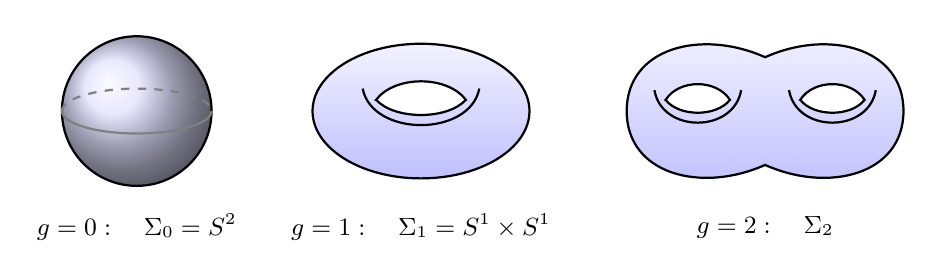
\begin{tikzpicture}[
  scale=0.95,
  line width=0.8pt,
  every node/.style={font=\small}
]

% g=0：球面
\begin{scope}
  \shade[ball color=blue!12] (0,0) circle (1);
  \draw (0,0) circle (1);

  % 赤道：手前は実線, 奥は破線
  \draw[dashed,gray]
    (-1,0) arc[start angle=180,end angle=0,
              x radius=1,y radius=0.3];
  \draw[gray]
    (-1,0) arc[start angle=180,end angle=360,
              x radius=1,y radius=0.3];

  \node at (0,-1.55) {$g=0:\quad \Sigma_0=S^2$};
\end{scope}

% g=1：トーラス
\begin{scope}[shift={(3.8,0)}]
  \shade[top color=blue!5,bottom color=blue!25]
    (0,0) ellipse[x radius=1.45,y radius=0.9];
  \draw (0,0) ellipse[x radius=1.45,y radius=0.9];

  % 穴
  \filldraw[fill=white]
    (-0.6,0.15)
    .. controls (-0.35,0.48) and (0.35,0.48) .. (0.6,0.15)
    .. controls (0.35,-0.12) and (-0.35,-0.12) .. cycle;

  % 穴の手前の曲面
  \draw
    (-0.78,0.30)
    .. controls (-0.65,-0.35) and (0.65,-0.35) .. (0.78,0.30);

  \node at (0,-1.55)
    {$g=1:\quad \Sigma_1=S^1\times S^1$};
\end{scope}

% g=2：二つの取っ手をもつ曲面
\begin{scope}[shift={(8.4,0)}]
  \shade[top color=blue!5,bottom color=blue!25]
    (-1.85,0)
    .. controls (-1.85,0.85) and (-0.85,1.10) .. (0,0.72)
    .. controls (0.85,1.10) and (1.85,0.85) .. (1.85,0)
    .. controls (1.85,-0.85) and (0.85,-1.10) .. (0,-0.72)
    .. controls (-0.85,-1.10) and (-1.85,-0.85) .. cycle;

  \draw
    (-1.85,0)
    .. controls (-1.85,0.85) and (-0.85,1.10) .. (0,0.72)
    .. controls (0.85,1.10) and (1.85,0.85) .. (1.85,0)
    .. controls (1.85,-0.85) and (0.85,-1.10) .. (0,-0.72)
    .. controls (-0.85,-1.10) and (-1.85,-0.85) .. cycle;

  % 二つの穴
  \foreach \a in {-0.9,0.9}{
    \begin{scope}[shift={(\a,0)}]
      \filldraw[fill=white]
        (-0.43,0.15)
        .. controls (-0.25,0.43) and (0.25,0.43) .. (0.43,0.15)
        .. controls (0.25,-0.08) and (-0.25,-0.08) .. cycle;

      \draw
        (-0.58,0.28)
        .. controls (-0.48,-0.30) and (0.48,-0.30) .. (0.58,0.28);
    \end{scope}
  }

  \node at (0,-1.55) {$g=2:\quad \Sigma_2$};
\end{scope}

\end{tikzpicture}
\caption{種数 $0,1,2$ の向き付け可能な閉曲面の模式図.}
\label{fig-surfaces-topological}
\end{figure}


ホモロジー群の生成元は, 次のように理解できる.
$H_0(X,\Z)$ は一点の類 $[p]$ で生成され, 
$H_2(X,\Z)$ は向き付けられた曲面全体の類 $[X]$ で生成される.
また, 各取っ手を二つの方向に回る閉曲線を $a_i,b_i$ とすると, 
\[
H_1(X,\Z)
=\bigoplus_{i=1}^{g}\Z[a_i]
\oplus\bigoplus_{i=1}^{g}\Z[b_i]
\]
となる.
つまり, 取っ手一つにつき, 一次ホモロジーの生成元が二つ現れる.

\begin{figure}[htbp]
\centering
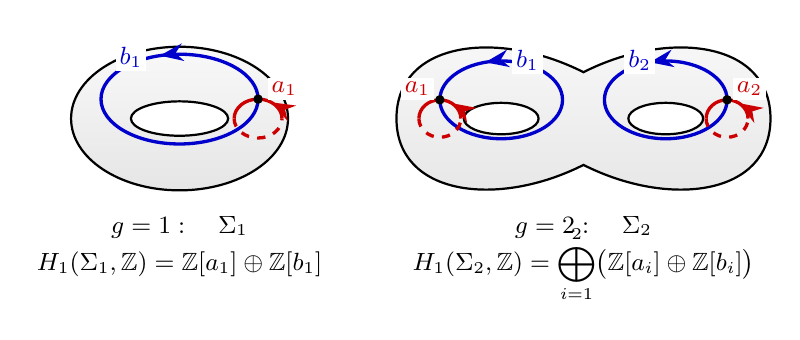
\begin{tikzpicture}[
  scale=0.95,
  line width=0.8pt,
  every node/.style={font=\small},
  directed/.style={
    postaction={decorate},
    decoration={
      markings,
      mark=at position 0.3 with {\arrow{Stealth}}
    }
  },
  aloop/.style={red!80!black,very thick},
  bloop/.style={blue!80!black,very thick},
  curve label/.style={fill=white,inner sep=1.5pt}
]

% ==================================================
% g=1：トーラス
% ==================================================
\begin{scope}

  % 曲面
  \shade[top color=gray!5,bottom color=gray!20]
    (0,0) ellipse[x radius=1.45,y radius=0.96];
  \draw
    (0,0) ellipse[x radius=1.45,y radius=0.96];

  % 中央の穴
  \filldraw[fill=white]
    (0,0) ellipse[x radius=0.65,y radius=0.23];

  % b_1：穴の周囲を回る閉曲線
  \draw[bloop,directed]
    (0,0.26) ellipse[x radius=1.05,y radius=0.60];

  % a_1：管を一周する閉曲線
  % 裏側
  \draw[aloop,dashed]
    (0.73,0)
    arc[start angle=180,end angle=360,
        x radius=0.32,y radius=0.26];

  % 表側
  \draw[aloop,directed]
    (1.37,0)
    arc[start angle=0,end angle=180,
        x radius=0.32,y radius=0.26];

  % 交点
  \fill (1.05,0.26) circle (1.8pt);

  % ラベル
  \node[curve label,text=red!80!black]
    at (1.40,0.40) {$a_1$};
  \node[curve label,text=blue!80!black]
    at (-0.65,0.82) {$b_1$};

  \node at (0,-1.45) {$g=1:\quad \Sigma_1$};
  \node at (0,-1.95)
    {$H_1(\Sigma_1,\Z)=\Z[a_1]\oplus\Z[b_1]$};

\end{scope}

% ==================================================
% g=2：二つの取っ手をもつ曲面
% ==================================================
\begin{scope}[shift={(5.4,0)}]

  % 曲面の輪郭
  \shade[top color=gray!5,bottom color=gray!20]
    (-2.5,0)
    .. controls (-2.5,1.03) and (-1.15,1.20) .. (0,0.62)
    .. controls (1.15,1.20) and (2.5,1.03) .. (2.5,0)
    .. controls (2.5,-1.03) and (1.15,-1.20) .. (0,-0.62)
    .. controls (-1.15,-1.20) and (-2.5,-1.03) .. cycle;

  \draw
    (-2.5,0)
    .. controls (-2.5,1.03) and (-1.15,1.20) .. (0,0.62)
    .. controls (1.15,1.20) and (2.5,1.03) .. (2.5,0)
    .. controls (2.5,-1.03) and (1.15,-1.20) .. (0,-0.62)
    .. controls (-1.15,-1.20) and (-2.5,-1.03) .. cycle;

  % 二つの穴
  \foreach \c in {-1.1,1.1}{
    \filldraw[fill=white]
      (\c,0) ellipse[x radius=0.50,y radius=0.21];
  }

  % b_1, b_2
  \draw[bloop,directed]
    (-1.1,0.25) ellipse[x radius=0.82,y radius=0.52];
  \draw[bloop,directed]
    (1.1,0.25) ellipse[x radius=0.82,y radius=0.52];

  % a_1：左の取っ手の外側
  \draw[aloop,dashed]
    (-2.20,0)
    arc[start angle=180,end angle=360,
        x radius=0.28,y radius=0.25];
  \draw[aloop,directed]
    (-1.64,0)
    arc[start angle=0,end angle=180,
        x radius=0.28,y radius=0.25];

  % a_2：右の取っ手の外側
  \draw[aloop,dashed]
    (1.64,0)
    arc[start angle=180,end angle=360,
        x radius=0.28,y radius=0.25];
  \draw[aloop,directed]
    (2.20,0)
    arc[start angle=0,end angle=180,
        x radius=0.28,y radius=0.25];

  % 各取っ手での交点
  \fill (-1.92,0.25) circle (1.8pt);
  \fill ( 1.92,0.25) circle (1.8pt);

  % ラベル
  \node[curve label,text=red!80!black]
    at (-2.22,0.40) {$a_1$};
  \node[curve label,text=red!80!black]
    at (2.22,0.40) {$a_2$};

  \node[curve label,text=blue!80!black]
    at (-0.75,0.78) {$b_1$};
  \node[curve label,text=blue!80!black]
    at (0.75,0.78) {$b_2$};

  \node at (0,-1.45) {$g=2:\quad \Sigma_2$};
  \node at (0,-1.95)
    {$H_1(\Sigma_2,\Z)
      =\displaystyle\bigoplus_{i=1}^{2}
        \bigl(\Z[a_i]\oplus\Z[b_i]\bigr)$};

\end{scope}

\end{tikzpicture}
\caption{曲面上の一次ホモロジーの生成元の模式図.
各取っ手で $a_i$ と $b_i$ は一点で交わる.
破線は曲面の裏側を通る部分を表す.}
\label{fig-homology-generators}
\end{figure}


\begin{rem}[位相的種数と解析的種数]
ここで定義した取っ手の個数を, 位相的種数 $g_{\mathrm{top}}(X)$ と呼ぶ.
一方, 第 \ref{O-S043} 章では
$g(X)=\dim_\C H^1(X,\mathcal O_X)$ によって解析的に種数を定義する.
定理 \ref{O-M305} で,
\[
g(X)=g_{\mathrm{top}}(X)
=\frac{2-\chi(X)}2=\frac12 b_1(X)
\]
を示す. 従って, 二つの定義は同じ整数を与える.
\end{rem}

\begin{exa}[球面とトーラス]
Riemann 球面 $\C\mathbb P^1$ は $S^2$ と同相なので, 
\[
g=0,\qquad \chi(\C\mathbb P^1)=2,\qquad
H_1(\C\mathbb P^1,\Z)=0
\]
である.

一方, 複素トーラス $E=\C/\Lambda$ は
$S^1\times S^1$ と同相なので, 
\[
g=1,\qquad \chi(E)=0,\qquad
H_1(E,\Z)\cong\Z^2
\]
である.
\end{exa}

\begin{exa}[超楕円曲線の種数]\label{O-M175}
\ref{O-S029} 節で構成した超楕円曲線
\[
C=\left(y^2=\prod_{i=1}^{2g+2}(x-a_i)\right)
\]
のEuler数と種数は
\[
\chi(C)=2-2g,\qquad \operatorname{genus}(C)=g
\]
である.
従って, $C$ は $\Sigma_g$ と同相である.
これは後にやるRiemann--Hurwitzの公式定理\ref{O-M306}から
$$
\chi(C)
= 
2 \times \chi(\C\mathbb P^1) - \sum_{\text{分岐点}} (2-1)
=2 \times 2 - (2g+2) = 2-2g
$$
となることからわかる. 
\end{exa}

\begin{rem}
ここでの分類は, 位相空間としての分類である.\footnote{知らなかったが微分同相での分類でもあるらしい. 曲面の分類を, 同相写像だけでなく微分同相写像を使って行えるから？}
同じ種数のコンパクトRiemann 面は同相だが, 
双正則同型であるとは限らない.これがRiemann 面のモジュライ・複素構造の話になっていく. 
\end{rem}



\newpage
% SOURCE O:4558 | O-S032 層と層係数コホモロジー群
\section{層と因子}\label{O-S032}

おそらく代数以外の分野の人が一番詰まるのが層(sheaf)であると思う.
なぜなら定義が無味乾燥としているからである. 集合と位相の授業を受けているかのように, わからなかったら定義に戻ってほしい. なぜなら定義以上のことは何もしておらず, ただ言い換えているだけだからである. 

\subsection{なぜ層を考えるのか？}
ここでは, 後で定義する層とコホモロジーの使い方を先に紹介する. 記号の意味は定義\ref{O-M199}, 例\ref{O-M187}, 定理\ref{O-M234}で説明する.


楕円曲線 $E=\C/\Lambda$ 上で, 指定した一点にだけ
$2$ 位の極をもつ有理型関数を作ることを考えよう.
すでにWeierstrassの $\wp$ 関数によって, 
そのような関数を具体的に構成した.
あの級数を思い付くのは容易ではないし, コンパクトRiemann 面ごとに関数を作るのはいい方法とはいえない. 
もっとシステマティックに関数の存在を示すことはできないだろうか？

層とコホモロジーを使うとシステマティックにわかるのである. つまり
\begin{tcolorbox}[mybox]
\begin{center}
ある点で極を持つ有理型関数が存在するかという問題を　\\
線形写像の核の次元を調べる問題に置き換えられる.
\end{center}
\end{tcolorbox}

具体例を楕円曲線で与えよう. 初読では考え方をつかみ, ある程度読み終えてから戻って確認すればよい.

$p\in E$ を固定し, その局所座標を $\varphi$, 座標変数を $z$ とする.
補題 \ref{O-M210} より, 短完全系列
\[
0\longrightarrow\mathcal O_E
\longrightarrow\mathcal O_E(2p)
\longrightarrow\C\{z\}/(z^2)
\longrightarrow0
\]
がある.
右端は $p$ に集中した摩天楼層である.例\ref{O-M187}の記法を用いている. 正確には, 開集合が $p$ を含めば $\C\{z\}/(z^2)$, 含まなければ $0$ を対応させる層である.

局所的に
\[
f=\frac{a_{-2}}{z^2}+\frac{a_{-1}}z+h(z)
\]
と書けば, 右向きの写像は
\[
f\longmapsto a_{-2}+a_{-1}z\bmod(z^2)
\]
である.
つまり, 極の部分の二つの係数を取り出している.

局所的に指定した極の部分が, 必ず $E$ 全体の有理型関数から得られるとは限らない.
この障害を記録するのが, コホモロジーである.

定理\ref{O-M234}のコホモロジー長完全系列と, 系\ref{O-M067}を使うと, 
\[
0\longrightarrow\C
\longrightarrow H^0(E,\mathcal O_E(2p))
\longrightarrow\C\{z\}/(z^2)
\xrightarrow{\delta}H^1(E,\mathcal O_E)
\]
を得る.
ここで $H^0(E,\mathcal O_E(2p))$ は, 
$p$ に高々 $2$ 位の極をもち, ほかでは正則な
大域的有理型関数の空間である.
完全性は, 局所的な極の部分が大域的な関数から得られることと, 
その $\delta$ による像が $0$ であることが同値だと述べている.

楕円曲線では, 例\ref{O-M299}と種数の定理\ref{O-M244}により
\[
\dim_\C H^1(E,\mathcal O_E)=1
\]
である.
一方, $\C\{z\}/(z^2)$ は $2$ 次元なので, 
\[
\dim_\C\operatorname{Ker}\delta\geq1.
\]
従って, 零でない極の部分をもつ大域的有理型関数が存在する.
この関数は定数ではなく, 極は $p$ にしかない.
さらに, 補題 \ref{O-M140} より, 
楕円曲線上に単純極を一つだけもつ有理型関数は存在しない.
従って, その極の位数はちょうど $2$ である.

こうして, $\wp$ 関数の級数表示を使わずに, 
同じ極の条件を満たす関数の存在がわかる.
層は局所的な条件を整理し, コホモロジーは
それを大域的に実現する際の障害を記録する.
その障害の空間の次元がわかれば, 
関数の存在を線形代数によって示せるのである.


\subsection{前層}\label{O-S033}

\begin{dfn}[前層]\label{O-M177}
$X$ を位相空間とする.
次のデータからなるものを, 
$X$ 上の $\C$-線形空間の前層 $\mathcal F$ という：
\begin{itemize}
\item 各開集合 $U\subset X$ に対する $\C$-線形空間 $\mathcal F(U)$.
\item 開集合の包含 $V\subset U$ に対する線形写像
\[
r^{\mathcal F}_{VU}:\mathcal F(U)\longrightarrow\mathcal F(V).
\]
\end{itemize}
これらには, 次の条件を課す：
\begin{enumerate}
\item $\mathcal F(\emptyset)=\{0\}$.
\item $r^{\mathcal F}_{UU}=\mathrm{id}_{\mathcal F(U)}$.
\item $W\subset V\subset U$ に対して
\[
r^{\mathcal F}_{WU}
=r^{\mathcal F}_{WV}\circ r^{\mathcal F}_{VU}.
\]
すなわち, 次の図式は可換である.
\[
\begin{tikzcd}[column sep=large,row sep=large]
\mathcal F(U)\arrow[r,"r^{\mathcal F}_{VU}"]\arrow[dr,"r^{\mathcal F}_{WU}"']
&\mathcal F(V)\arrow[d,"r^{\mathcal F}_{WV}"]\\
&\mathcal F(W)
\end{tikzcd}
\]

\end{enumerate}

$\mathcal F(U)$ の元を $U$ 上の切断といい, 
$r^{\mathcal F}_{VU}$ を制限写像という.
また, 
\[
\Gamma(U,\mathcal F):=\mathcal F(U),\qquad
s|_V:=r^{\mathcal F}_{VU}(s)
\]
とも書く.
\end{dfn}

\begin{exa}[連続関数の前層]\label{exa-continuous-presheaf}
$X$ を位相空間とする.
各開集合 $U\subset X$ に対して, 
\[
\mathcal C_X^0(U)
:=\{f:U\to\C\mid f\text{ は連続}\}
\]
とおく.
また, $V\subset U$ に対して, 制限写像を
\[
r_{VU}:\mathcal C_X^0(U)\longrightarrow\mathcal C_X^0(V),
\qquad f\longmapsto f|_V
\]
と定める.
このとき, $\mathcal C_X^0$ は $X$ 上の前層である.
\end{exa}

\begin{proof}
まず, 連続関数の和と複素数倍は連続なので, 
$\mathcal C_X^0(U)$ は $\C$-線形空間である.
また, 連続関数の制限は連続なので, $r_{VU}$ は定義でき, 
\[
(\alpha f+\beta g)|_V
=\alpha f|_V+\beta g|_V
\qquad(\alpha,\beta\in\C)
\]
より線形写像である.

前層の三つの条件を確認する.
\begin{enumerate}
\item
空集合から $\C$ への関数は一つだけである.
これを零元とみなすと, 
$\mathcal C_X^0(\emptyset)=\{0\}$ となる.

\item
$f|_U=f$ なので, $r_{UU}=\mathrm{id}$ である.

\item
$W\subset V\subset U$ ならば
\[
(f|_V)|_W=f|_W
\]
なので, $r_{WV}\circ r_{VU}=r_{WU}$ である.
\end{enumerate}
従って, 前層の定義のすべての条件を満たす.
\end{proof}

\begin{exa}[$C^\infty$ 級関数の前層]
$X$ をRiemann 面とし, その下部の $C^\infty$ 級構造を考える.
各開集合 $U\subset X$ に対して, 
\[
A_X^0(U)
:=\{f:U\to\C\mid f\text{ は }C^\infty\text{ 級}\}
\]
とおく.
通常の制限写像
\[
r_{VU}:A_X^0(U)\longrightarrow A_X^0(V),
\qquad f\longmapsto f|_V
\]
によって, $A_X^0$ は前層となる.
\end{exa}

\begin{proof}
$C^\infty$ 級関数の和, 複素数倍, 開集合への制限は, 
いずれも $C^\infty$ 級である.
従って, $A_X^0(U)$ は $\C$-線形空間であり, 
$r_{VU}$ は線形写像である.
さらに, 連続関数の場合と同様に, 
\[
A_X^0(\emptyset)=\{0\},\qquad
r_{UU}=\mathrm{id},\qquad
r_{WV}\circ r_{VU}=r_{WU}
\]
が成り立つので, 前層である.
\end{proof}

\begin{rem}[これまでに登場した前層]\label{exa-holomorphic-presheaf}
本書で扱ってきた関数や微分形式も, 
各開集合上のものを集め, 通常の制限写像を使うことで前層となる.
例えば, 次はいずれも $X$ 上の前層である：
\[
\begin{array}{c|l}
\text{開集合 }U\text{ に対応する線形空間}
& \text{その元}\\ \hline
\mathcal O_X(U) & U\text{ 上の正則関数}\\
\mathcal M_X(U) & U\text{ 上の有理型関数}\\
A_X^1(U) & U\text{ 上の }C^\infty\text{ 級 }1\text{ 形式}\\
A_X^2(U) & U\text{ 上の }C^\infty\text{ 級 }2\text{ 形式}\\
A_X^{1,0}(U) & U\text{ 上の }C^\infty\text{ 級 }(1,0)\text{ 形式}\\
A_X^{0,1}(U) & U\text{ 上の }C^\infty\text{ 級 }(0,1)\text{ 形式}\\
\Omega_X^1(U) & U\text{ 上の正則 }1\text{ 形式}
\end{array}
\]
有理型 $1$ 形式についても同様である.
いずれも加法・複素数倍・制限でその性質が保たれ, 
制限を繰り返す規則は連続関数の場合と同じだからである.
空集合上では, すべて $\{0\}$ とする.
\end{rem}


\begin{dfn}[前層の準同型と同型]\label{O-M181}\label{O-M183}
$\mathcal F,\mathcal G$ を $X$ 上の前層とする.
\begin{enumerate}
\item
各開集合 $U\subset X$ に対する線形写像
\[
\varphi(U):\mathcal F(U)\longrightarrow\mathcal G(U)
\]
の集まりが, 任意の開集合 $V\subset U$ に対して
\[
\varphi(V)\circ r^{\mathcal F}_{VU}
=r^{\mathcal G}_{VU}\circ\varphi(U)
\]
を満たすとき, 前層の準同型といい, 
$\varphi:\mathcal F\to\mathcal G$ と書く.
つまり, $\varphi$ は制限と両立する：
\[
\varphi(s|_V)=\varphi(s)|_V.
\]
\[
\begin{tikzcd}[column sep=large,row sep=large]
\mathcal F(U)\arrow[r,"\varphi(U)"]\arrow[d,"r^{\mathcal F}_{VU}"']
&\mathcal G(U)\arrow[d,"r^{\mathcal G}_{VU}"]\\
\mathcal F(V)\arrow[r,"\varphi(V)"']&\mathcal G(V)
\end{tikzcd}
\]


\item
準同型の合成と恒等写像は, 各開集合上で
\[
(\psi\circ\varphi)(U)=\psi(U)\circ\varphi(U),\qquad
\mathrm{id}_{\mathcal F}(U)=\mathrm{id}_{\mathcal F(U)}
\]
と定める.
\[
\begin{tikzcd}[column sep=large]
\mathcal F(U)\arrow[r,"\varphi(U)"]\arrow[rr,bend right=25,"(\psi\circ\varphi)(U)"']
&\mathcal G(U)\arrow[r,"\psi(U)"]&\mathcal H(U)
\end{tikzcd}
\]



\item
すべての開集合 $U$ で $\varphi(U)$ が線形同型であるとき, 
$\varphi$ を前層の同型という.
このような同型が存在するとき, 
$\mathcal F\simeq\mathcal G$ と書く.

\end{enumerate}
\end{dfn}

\begin{exa}
正則関数を同じ $C^\infty$ 級関数とみなす対応は, 
前層の準同型
\[
\iota:\mathcal O_X\longrightarrow A_X^0
\]
を定める.
\end{exa}

\begin{proof}
定義 \ref{O-M181} の条件を順に確認する.

まず, 正則関数は $C^\infty$ 級なので, 
各開集合 $U\subset X$ に対して
\[
\iota(U):\mathcal O_X(U)\longrightarrow A_X^0(U),
\qquad f\longmapsto f
\]
が定まる.
$\iota(U)$ は線形写像である.

次に, 開集合 $V\subset U$ を取る.
両前層の制限写像は, 関数の定義域を $V$ に制限する写像なので, 
任意の $f\in\mathcal O_X(U)$ に対して
\[
\begin{aligned}
(\iota(V)\circ r^{\mathcal O_X}_{VU})(f)
=\iota(V)(f|_V)=f|_V, \qquad
(r^{A_X^0}_{VU}\circ\iota(U))(f)
=r^{A_X^0}_{VU}(f)=f|_V
\end{aligned}
\]
となる.従って, 
\[
\iota(V)\circ r^{\mathcal O_X}_{VU}
=r^{A_X^0}_{VU}\circ\iota(U)
\]
が成り立つ. \[
\begin{tikzcd}[column sep=large,row sep=large]
\mathcal O_X(U)\arrow[r,hook,"\iota(U)"]\arrow[d,"\text{制限}"']
&A_X^0(U)\arrow[d,"\text{制限}"]\\
\mathcal O_X(V)\arrow[r,hook,"\iota(V)"']&A_X^0(V)
\end{tikzcd}
\]

よって, $\iota$ は前層の準同型である.
これは同型ではない. 正則ではない$C^\infty$級関数が存在するためである. 

\end{proof}



\begin{dfn}[芽とストーク]\label{O-M179}
$\mathcal F$ を $X$ 上の前層とし, $p\in X$ とする.
$p$ の開近傍 $U$ と切断 $s\in\mathcal F(U)$ の対 $(U,s)$ を考える.

二つの対 $(U,s),(V,t)$ に対し, 
\[
(U,s)\sim(V,t)
\iff
\begin{gathered}
p\in W\subset U\cap V\text{ となる開集合 }W\text{ が存在し, }\\
s|_W=t|_W
\end{gathered}
\]
と定める.
この同値関係による同値類を $p$ における芽(germ)といい, 
$(U,s)$ の定める芽を $s_p$ と書く.

芽全体の集合
\[
\mathcal F_p
:=
\{(U,s)\mid U\text{ は }p\text{ の開近傍},\
s\in\mathcal F(U)\}/\sim
\]
を, $p$ における $\mathcal F$ のストーク(stalk)という.
\end{dfn}


\begin{exa}[$C^\infty$ 級関数の芽とストーク]
$A_X^0$ を $C^\infty$ 級関数の前層とする.
その $p$ におけるストーク $(A_X^0)_p$ は, 
$p$ の近傍で定義された $C^\infty$ 級関数を, 
十分小さい近傍で一致するときに同一視したものである.

これは定義\ref{dfn-smooth-germ}の $C^\infty$ 級関数の芽全体
$A^0_{X,p}$ にほかならない.従って, 
\[
(A_X^0)_p=A^0_{X,p}
\]
である.
以前の記号 $[f]$ は, 前層の記号では $f_p$ に当たる.
以下, 同じ芽を $[f]=f_p$ と書き, $(A_X^0)_p=A^0_{X,p}$ と同一視する.


例えば, $p\in V\subset U$ とし, 
$f\in A_X^0(U)$, $g=f|_V$ とすると, 
定義域は異なっていても
\(
f_p=g_p
\)
である.
一方, $X=\C$, $p=0$ における $f(z)=z$ と $h(z)=0$ は, 
$f(0)=h(0)$ だが, どの近傍でも一致しないので
\(
f_0\neq h_0
\)
である.芽は, 一点での値だけでなく, その近くでの関数を記録する.
\end{exa}
定義\ref{O-M179}から次がわかる.
\begin{lem}[芽の一致とストークの演算]\label{lem-stalk-germs}
芽の一致は
\[
s_p=t_p
\quad\Longleftrightarrow\quad
p\text{ のある開近傍で }s=t
\]
を意味する.
特に, $s_p=0$ とは, $s$ が $p$ のある開近傍上で
零切断になることである.

ストークには自然に線形空間の構造が入る.
$s\in\mathcal F(U)$, $t\in\mathcal F(V)$, 
$\alpha,\beta\in\C$ に対して, 
\[
\alpha s_p+\beta t_p
:=
\left(\alpha\,s|_{U\cap V}
+\beta\,t|_{U\cap V}\right)_p
\]
と定めればよい.
つまり, 共通の近傍に制限してから演算する.
この定義は代表元の選び方によらず, 
自然な写像
\[
\mathcal F(U)\longrightarrow\mathcal F_p,\qquad
s\longmapsto s_p
\quad(p\in U)
\]
も線形写像となる.
\end{lem}

\begin{exa}[$C^\infty$ 級関数の芽の演算]
$X=\C$, $p=0$ とする. $f(z)=|z|^2$, $g(z)=1+z$ を
それぞれ原点の近傍 $U,V$ で考えると, 補題\ref{lem-stalk-germs}の演算は
\[
2f_0-g_0=(2|z|^2-1-z)_0
\]
である. 右辺は共通の近傍 $U\cap V$ 上の関数の芽であり,
代表元の定義域を小さくしても変わらない.
一方, $f(0)=0$ でも $f$ は原点のどの近傍でも零関数でないので,
$f_0\neq0$ である.
\end{exa}



\begin{rem}
前層の同型は, 各点でストークの同型
\(
\varphi_p:\mathcal F_p\xrightarrow{\sim}\mathcal G_p
\)
を誘導する.
\end{rem}




\begin{dfn}[前層のサポート]\label{O-M180}
前層 $\mathcal F$ に対して, 
\[
\operatorname{Supp}\mathcal F
:=\{p\in X\mid\mathcal F_p\neq\{0\}\}
\]
を $\mathcal F$ のサポートという.
つまり, 零でない芽が存在する点全体である.
\end{dfn}


\begin{exa}[関数の前層のサポート]
連続関数, $C^\infty$ 級関数, 正則関数, 有理型関数の前層は, 
いずれもサポートが $X$ 全体である.すなわち, 
\[
\operatorname{Supp}\mathcal C_X^0
=\operatorname{Supp}A_X^0
=\operatorname{Supp}\mathcal O_X
=\operatorname{Supp}\mathcal M_X
=X.
\]

実際, 定数関数 $1$ は, どの点 $p$ の近傍に制限しても
零関数にはならない.
従って, その芽 $1_p$ はどのストークでも非零であり, 
すべての点 $p\in X$ がサポートに属する.
\end{exa}

\begin{exa}[一点にサポートをもつ前層：摩天楼層]\label{O-M186}
$X$ をRiemann 面とし, $p\in X$ を固定する.
各開集合 $U\subset X$ に対して, 
\[
\C_p(U):=
\begin{cases}
\C & p\in U,\\
\{0\} & p\notin U
\end{cases}
\]
と定める.
つまり, $p$ を含む開集合上では一つの複素数をデータとしてもち, 
$p$ を含まない開集合上では零元しかもたない.

$V\subset U$ に対する制限写像は
\[
r_{VU}:\C_p(U)\longrightarrow\C_p(V),\qquad
r_{VU}=
\begin{cases}
\mathrm{id}_{\C} & p\in V,\\
0 & p\notin V
\end{cases}
\]
とする.
このデータは前層を定め, そのストークとサポートは
\[
(\C_p)_q\cong
\begin{cases}
\C & q=p,\\
\{0\} & q\neq p,
\end{cases}
\qquad
\operatorname{Supp}\C_p=\{p\}
\]
である.
これは後で定義する層の条件も満たし, 
$p$ にサポートをもつ摩天楼層
（skyscraper sheaf）と呼ばれる.

実際, $q=p$ の場合, 近傍上の切断は複素数 $c$ であり,
近傍を小さくしても制限は恒等写像なので同じ $c$ が残る.
従って芽を $c$ に対応させると $(\C_p)_p\cong\C$ となる.
$q\neq p$ ならば, $p$ を含まない $q$ の近傍 $W$ を取れる.
任意の切断を $W$ と共通の近傍に制限すると零になるので,
補題\ref{lem-stalk-germs}よりすべての芽が零である.

\end{exa}

\begin{rem}[前層の圏論的な定義]
圏論が好きな人は下の定義の方がいいかもしれない. 以下この圏論的な定義を書くがわからない人は無視して良い. 

\begin{defn}
$X$ の開集合全体を圏 $\operatorname{Open}(X)$ とみなす.
その対象は開集合であり, 射は包含に対応する：
\[
\operatorname{Hom}_{\operatorname{Open}(X)}(V,U)
=
\begin{cases}
\{\text{包含写像 }V\hookrightarrow U\} & V\subset U,\\
\emptyset & V\not\subset U.
\end{cases}
\]
また, $\operatorname{Vect}_{\C}$ を複素線形空間と線形写像の圏とする.

$X$ 上の複素線形空間の前層とは, 反変関手
\[
\mathcal F:\operatorname{Open}(X)^{\mathrm{op}}
\longrightarrow\operatorname{Vect}_{\C}
\]
のことである.
すなわち, 開集合 $U$ に線形空間 $\mathcal F(U)$ を, 
包含 $V\hookrightarrow U$ に逆向きの線形写像
\[
r_{VU}:\mathcal F(U)\longrightarrow\mathcal F(V)
\]
を対応させる.
関手の公理は, ちょうど制限写像の条件
\[
r_{UU}=\mathrm{id}_{\mathcal F(U)},\qquad
r_{WV}\circ r_{VU}=r_{WU}\quad(W\subset V\subset U)
\]
に当たる.
なお, 本書ではさらに $\mathcal F(\emptyset)=\{0\}$ を課しているが, 
これは関手の公理だけからは従わない.

前層の準同型 $\varphi:\mathcal F\to\mathcal G$ は, 
これらの関手の間の自然変換である.
その自然性の条件は
\[
\varphi(V)\circ r^{\mathcal F}_{VU}
=
r^{\mathcal G}_{VU}\circ\varphi(U)
\]
であり, 前層の準同型が制限写像と両立するという条件そのものである.
前層の同型は自然同型に当たる.

この見方では, 点 $p\in X$ におけるストークは
\[
\mathcal F_p
\cong
\varinjlim_{U\ni p}\mathcal F(U)
\]
という帰納極限で表される.
ここでは, $p$ の開近傍を対象とし, 
$V\subset U$ のとき $U\to V$ という射を入れて, 
制限写像に沿って極限を取る.
二つの切断を, 十分小さい共通の近傍で一致するときに
同一視することが, 芽による定義に対応している.
\end{defn}
終域の圏を集合の圏, Abel群の圏, 環の圏などに替えれば, 
それぞれの値を取る前層も同様に定義できる.

この定義で気づいた方もいるかもしれないが, 前層の定義での"開集合全体を圏 $\operatorname{Open}(X)$"は別に一般の圏に変えても差し支えないことがわかる. 
ではこの後の"層"も一般の圏に変えることができるのではないか？
これはYesであり, "圏"にGrothendieck位相を入れたらGrothendieckトポス(圏の層)が考えられる. 
\footnote{私はショルツのcondensed mathmaticsを学んだときにGrothendieckトポスを知ったが, このあたり非常に難しい. condenced setを"Profinite setのなす圏にGrothendieck位相を入れ, そのSet値の層"として定義する. これで理解できる人は果たして何人いるのだろうか??}
\end{rem}
% SOURCE O:4564 | O-S033 層
\subsection{層}\label{sec-sheaves}

\begin{dfn}[層]\label{O-M184}
$X$ 上の前層 $\mathcal F$ が次の二つの条件を満たすとき, 
$\mathcal F$ を層という.
ここで, $U\subset X$ は任意の開集合, 
$U=\bigcup_{i\in I}U_i$ はその任意の開被覆とする.
\begin{enumerate}
\item

$s,t\in\mathcal F(U)$ に対して, 
\[
s|_{U_i}=t|_{U_i}\qquad(i\in I)
\]
ならば, $s=t$ である.

\item

共通部分で一致する切断は貼りあわせられる.
各 $U_i$ 上の切断 $s_i\in\mathcal F(U_i)$ が
\[
s_i|_{U_i\cap U_j}=s_j|_{U_i\cap U_j}
\qquad(i,j\in I)
\]
を満たすならば, 
\[
s|_{U_i}=s_i\qquad(i\in I)
\]
となる切断 $s\in\mathcal F(U)$ が存在する.
\end{enumerate}

層のストーク, サポート, 準同型, 同型は, 
それぞれ前層として定義したものを用いる.
これらの定義は, 定義\ref{O-M181}, 定義\ref{O-M179}, 定義\ref{O-M180}を参照されたい.

\end{dfn}


\begin{exa}
例\ref{exa-continuous-presheaf}でやった連続関数の前層 $\mathcal C_X^0$ は層である.
\end{exa}

\begin{proof}
$U=\bigcup_i U_i$ を任意の開被覆とする.
層の二つの条件を確認する.
定義\ref{O-M184}の (1), (2) を順に示す.

(1) $f,g\in\mathcal C_X^0(U)$ が各 $U_i$ 上で一致すれば, 
$U$ のすべての点で値が一致するので, $f=g$ である.

(2) 各 $U_i$ 上の連続関数 $f_i$ が共通部分で一致するとする.
$p\in U$ に対し, $p\in U_i$ となる $i$ を選び, 
\[
f(p):=f_i(p)
\]
と定める.
共通部分では $f_i=f_j$ なので, この値は $i$ の選び方によらず, 
$f|_{U_i}=f_i$ となる.

この $f$ は連続である.
実際, 任意の開集合 $G\subset\C$ に対して
\[
f^{-1}(G)=\bigcup_i f_i^{-1}(G)
\]
であり, 各 $f_i^{-1}(G)$ は $U_i$ の開集合である.
$U_i$ は $U$ で開いているので, 右辺は $U$ の開集合である.
従って $f\in\mathcal C_X^0(U)$ であり, 貼りあわせが得られる.
\end{proof}


\begin{exa}[正則関数の層]\label{O-M185}
補足\ref{exa-holomorphic-presheaf}でやったRiemann 面 $X$ 上の正則関数の前層 $\mathcal O_X$ は層である.
\end{exa}

\begin{proof}
$U=\bigcup_i U_i$ を開被覆とする.
定義\ref{O-M184}に従い, 一致と貼りあわせを確認する.

(1) $f,g\in\mathcal O_X(U)$ が各 $U_i$ 上で一致すれば, 
$U$ の各点で $f=g$ なので, $U$ 全体で一致する.

(2) $f_i\in\mathcal O_X(U_i)$ が共通部分で一致するとする.
$p\in U$ に対して, $p\in U_i$ となる $i$ を選び, 
\[
f(p):=f_i(p)
\]
と定める.
共通部分での一致により, この値は $i$ の選び方によらない.
任意の $p\in U$ に対し $p\in U_i$ を選ぶと, $p$ の開近傍 $U_i$ で $f=f_i$ である. 正則性は各点の近傍で判定でき, $f_i$ は正則なので, $f$ も $U$ 上で正則である.
従って, $f\in\mathcal O_X(U)$ は求める貼りあわせである.
\end{proof}

\begin{exa}[関数と微分形式の層]
次の前層も, 通常の制限写像によって層になる.
\begin{itemize}
\item 零切断だけからなる層 $0$.
\item 連続関数の層 $\mathcal C_X^0$.
\item $C^\infty$ 級関数の層 $A_X^0$.
\item 有理型関数の層 $\mathcal M_X$.
\item 正則 $1$ 形式の層 $\Omega_X^1$.
\item $C^\infty$ 級 $n$ 形式の層 $A_X^n$（$n=1,2$）.
\item $C^\infty$ 級 $(1,0)$ 形式, $(0,1)$ 形式の層
$A_X^{1,0},A_X^{0,1}$.
\item 複素数値の局所定数関数の層 $\C_X$.
\end{itemize}

\end{exa}


\begin{exa}[層の準同型]
二つの基本的な準同型を挙げる. いずれも定義\ref{O-M181}の制限との両立を満たす.

正則関数を $C^\infty$ 級関数とみなす包含
\[
\iota:\mathcal O_X\longrightarrow A_X^0
\]
は層の準同型である.
実際, 各開集合上で線形であり, 
\[
\iota(f|_V)=\iota(f)|_V
\]
と制限に両立する.

また, 外微分も層の準同型
\[
d:A_X^0\longrightarrow A_X^1
\]
を定める.
実際, 外微分は複素線形であり, 
開集合 $V\subset U$ と $f\in A_X^0(U)$ に対して
\[
d(f|_V)=(df)|_V
\]
が成り立つ.
\end{exa}


\begin{exa}[前層だが層でない例]
有界性は開集合全体に関する条件なので, 局所的に成り立っても全体で成り立つとは限らない. 次の例では, 定義\ref{O-M184} (2) が破れる.

$X=\R$ とし, 各開集合 $U\subset\R$ に対して
\[
\mathcal B(U)
:=\{f:U\to\C\mid f\text{ は有界}\}
\]
とおく.
有界関数の制限は有界なので, 通常の制限写像により
$\mathcal B$ は前層となる.

しかし, $\mathcal B$ は層ではない.
実際, 開被覆
\[
\R=\bigcup_{n\geq1}U_n,\qquad U_n=(-n,n)
\]
を取り, $f_n(x)=x$ とおく.
各 $f_n$ は $U_n$ 上で有界であり, 共通部分でも一致する.

これらを貼りあわせる関数 $f:\R\to\C$ は, 
すべての $U_n$ 上で $f(x)=x$ を満たすので, 
$\R$ 全体で $f(x)=x$ でなければならない.
ところが, この関数は有界でないため, 
$f\notin\mathcal B(\R)$ である.
従って, 層の貼りあわせの存在条件を満たさない.
\end{exa}



次は層にあって前層にはない大切な性質の $1$ つである.\footnote{このあたり前層の全射と層の全射が違うなど, 代数が好きな人には面白いところである. epiとかmonoとか圏論っぽい話である. が, ちょっとマニアックすぎるので, この授業では触れない. }

% SOURCE O:4917 | O-M191 eg 5.13; original option: 5.13
\begin{lem}\label{O-M191}
$X$ を位相空間とする. $\mathcal{F}$, $\mathcal{G}$ を $X$ 上の層とする. $\varphi:\mathcal{F}\to\mathcal{G}$ を層の準同型写像とする. $\varphi$ について, 次の (1) と (2) は同値である:
\begin{enumerate}
\item[(1)]
$\varphi$ は同型写像.
\item[(2)]
$X$ のすべての点 $p$ に対して $\varphi$ の導くストークの間の写像
\(
\varphi_p:\mathcal{F}_p\to\mathcal{G}_p
\)
は同型写像.
\end{enumerate}
\end{lem}
\begin{proof}
(1) から (2) は逆写像もストークに写せばよい. 逆に (2) を仮定する.
まず $\varphi(U)(s)=0$ ならば, 各点 $p\in U$ で
$\varphi_p(s_p)=0$ である. $\varphi_p$ の単射性から $s_p=0$ となり,
補題\ref{lem-stalk-germs}と層の一致条件より $s=0$ である.
従って, どの開集合 $U$ でも $\varphi(U)$ は単射である.

$t\in\mathcal G(U)$ を取る. $\varphi_p$ の全射性より,
各 $p\in U$ の十分小さい近傍 $U_p$ で
$\varphi(s^{(p)})=t|_{U_p}$ となる $s^{(p)}\in\mathcal F(U_p)$ が取れる.
共通部分ではこれらの像が同じなので, 今示した単射性から
$s^{(p)}|_{U_p\cap U_q}=s^{(q)}|_{U_p\cap U_q}$ である.
定義\ref{O-M184} (2) により $s^{(p)}$ は $s\in\mathcal F(U)$ に貼りあわさり,
同定義 (1) より $\varphi(s)=t$ となる. 従って $\varphi(U)$ は全単射である.
\end{proof}


最後に前層は層にできる. これを層化という. これは主張を書くだけにとどめる. \footnote{例えば, 層の準同型 $\mathcal F\to\mathcal G$ に対して, 開集合ごとの商 $\mathcal G(U)/\operatorname{Im}\mathcal F(U)$ は一般には層にならない. 余核の層はこの前層を層化して作る. テンソル積も同様に, 開集合ごとのテンソル積を層化して定める（定義\ref{rem-tensor-sheaves}参照）.
}
\begin{lem}[層化の存在と一意性]\label{O-M193}
$X$ 上の任意の前層 $\mathcal F$ に対して, 
層 $\mathcal F^a$ と前層の準同型
\[
\iota:\mathcal F\longrightarrow\mathcal F^a
\]
で, 次の性質を満たすものが存在する.

"任意の層 $\mathcal G$ と前層の準同型
$\varphi:\mathcal F\to\mathcal G$ に対して, 
\(
\varphi=\varphi^a\circ\iota
\)
となる層の準同型 $\varphi^a:\mathcal F^a\to\mathcal G$ が
一意に存在する."
\[
\begin{tikzcd}[column sep=large, row sep=large]
\mathcal F
  \arrow[r, "\iota"]
  \arrow[dr, swap, "\varphi"]
&
\mathcal F^a
  \arrow[d, dashed, "\exists!\,\varphi^a"]
\\
& \mathcal G
\end{tikzcd}
\]

この対 $(\mathcal F^a,\iota)$ を $\mathcal F$ の層化という.
層化は $\iota$ と両立する一意な同型を除いて一意であり, 
各点 $p\in X$ で自然な同型
\(
\mathcal F_p\xrightarrow{\;\sim\;}(\mathcal F^a)_p
\)
を誘導する.
\end{lem}


\begin{exa}[Abel群の層]\label{O-M189}
層の各開集合上の切断は, 線形空間ではなく
Abel群であってもよい.
Riemann 面 $X$ 上では, 次がその例である.
\begin{enumerate}
\item
整数の定数層(constant sheaf)を
\[
\Z_X(U)
:=\{f:U\to\Z\mid f\text{ は局所定数}\}
\]
とする.
通常の加法でAbel群となり, 単位元は定数関数 $0$ である.
ここで局所定数とは, 各点の十分小さい近傍で定数となることをいう.\footnote{Riemann 面では, $\Z_X$ を係数とする層コホモロジーは整数係数の特異コホモロジーと自然に同型になる. 後の例\ref{O-M212}も参照されたい.
}

\item

各開集合 $U$ に, 一元群
\[
1(U):=\{1\}
\]
を対応させる.
演算を乗法で書き, 唯一の元 $1$ を単位元とする.

\item

零点をもたない正則関数の層.
\[
\mathcal O_X^*(U)
:=\{f\in\mathcal O_X(U)\mid f(p)\neq0\text{ for all }p\in U\}
\]
とする.
通常の乗法でAbel群となり, 単位元は定数関数 $1$, 
$f$ の逆元は正則関数 $1/f$ である.
\end{enumerate}
いずれも通常の制限写像を用いる.
これらは$\C$-線形空間の層ではないがAbel群の層である. \footnote{特に $H^1(X,\mathcal O_X^*)$ は正則直線束の同型類を分類する. コンパクトRiemann 面では, これは因子の線形同値類の群とも同一視できる（例\ref{O-M212}参照）.
}

\end{exa}




\subsection{正則関数の層と摩天楼層のストーク}


正則関数の層 $\mathcal O_X$ は, 各開集合 $U\subset X$ に
\[
\mathcal O_X(U):=\{U\text{ 上の正則関数}\}
\]
を対応させる層である.
そのストーク $\mathcal O_{X,p}:=(\mathcal O_X)_p$ は, 
$p$ における正則関数の芽全体からなる.
局所座標を選ぶと, この芽をTaylor級数で表すことができる.

\begin{lem}[正則関数の芽と収束べき級数]\label{O-M190}

$p\in X$ とし, 局所座標 $\varphi$（座標変数 $z$）によって, 
$p$ の近傍を $\C$ の原点の近傍と同一視する.
このとき, Taylor展開によって
\[
\mathcal O_{X,p}\simeq\C\{z\}
\]
という $\C$-代数の同型が得られる.
ここで, 
\[
\C\{z\}
:=
\left\{
\sum_{k=0}^{\infty}a_kz^k
\ \middle|\
a_k\in\C,\ \text{収束半径が正}
\right\}
\]
は収束べき級数環である.
\end{lem}
\begin{proof}
正則関数のTaylor展開定理により, 
原点の近くで正則な関数 $f$ に対して, ある $r>0$ が存在し, 
\[
f(z)=\sum_{k=0}^{\infty}\frac{f^{(k)}(0)}{k!}z^k
\qquad(|z|<r)
\]
が成り立つ.
そこで, Taylor級数を対応させる写像
\[
\iota:\mathcal O_{X,p}\longrightarrow\C\{z\},
\qquad
[f]\longmapsto
\sum_{k=0}^{\infty}\frac{f^{(k)}(0)}{k!}z^k
\]
を考える.
同じ芽の代表元は原点の近くで一致するので, 
この写像は代表元の選び方によらない.

$\iota([f])=\iota([g])$ ならば, Taylor級数の係数が一致し,
\[
\frac{f^{(k)}(0)}{k!}=\frac{g^{(k)}(0)}{k!}
\qquad(k\geq0)
\]
となる.
正則関数は十分小さい近傍でそのTaylor級数の和に等しいので,
原点の近くで $f=g$ である.
従って $[f]=[g]$ となり, $\iota$ は単射である.

任意の収束べき級数 $\sum_{k=0}^{\infty}a_kz^k$ の和を $f$ とする.
$f$ は原点の近くで正則であり,
\[
\frac{f^{(k)}(0)}{k!}=a_k
\qquad(k\geq0)
\]
なので, $\iota([f])=\sum_{k=0}^{\infty}a_kz^k$ となる.
従って $\iota$ は全射である.

Taylor展開は加法, 複素数倍, 乗法を保つから, 
$\iota$ は $\C$-代数の同型である.
\end{proof}


正則性は必要である. $C^\infty$だと単射にならない. (解析関数$C^{\omega}$ならその心配はない. ) 

\begin{exa}[$C^\infty$ 級関数ではTaylor級数から芽は決まらない]

原点でのTaylor級数が正の収束半径をもつ
複素数値 $C^\infty$ 級関数の芽全体を $A_{\mathrm{conv}}$ とおく.
Taylor展開によって写像
\[
\iota:A_{\mathrm{conv}}\longrightarrow\C\{x\},
\qquad
[f]\longmapsto
\sum_{k=0}^{\infty}\frac{f^{(k)}(0)}{k!}x^k
\]
が定まるが, この写像は単射ではない.

実際, $\R$ 上の関数
\[
f(x)=
\begin{cases}
e^{-1/x^2} & x\neq0,\\
0 & x=0
\end{cases}
\]
を考える.
$x\neq0$ での各導関数は $1/x$ の多項式と
$e^{-1/x^2}$ の積であり, $x\to0$ のとき
任意の $|x|$ の正のべきよりも速く $0$ に近づく.
このことから, $f$ は $C^\infty$ 級であり, 
\[
f^{(k)}(0)=0\qquad(k\geq0)
\]
となる.
従って, $f$ のTaylor級数は零級数なので収束し, 
$\iota([f])=\iota([0])=0$ である.
しかし, $x\neq0$ では $f(x)>0$ なので, 
原点のどの近傍でも零関数とは一致せず, $[f]\neq[0]$ である.
\end{exa}


\begin{exa}[$\C\mathbb P^1$ 上の一点に集中した層]\label{exa-skyscraper-jets3}
$X=\C\mathbb P^1$, $p=[0:1]$ とし, $p$ の近くの座標変数を $z$ とする.
補題\ref{O-M190}の収束べき級数環を用いて,
\[
S(U)=\begin{cases}\C\{z\}/(z^3)&p\in U,\\0&p\notin U\end{cases}
\]
と定める. 制限写像は, 制限先が $p$ を含めば恒等写像, 含まなければ零写像である.
剰余類は一意に $a+bz+cz^2\pmod{z^3}$ と書ける. 特に,
\[
f(z)\equiv f(0)+f'(0)z+\frac{f''(0)}{2}z^2\pmod{z^3}
\]
なので, $S$ は一点での値と $2$ 階までの微分を記録する層である.
$p$ を含む開集合どうしでは, 貼りあわせる切断は同じ剰余類でなければならず,
その剰余類が一意な貼りあわせを与える. 従って層の条件を満たす.
例\ref{O-M186}と同様に,
\[
S_p\cong\C\{z\}/(z^3),\qquad S_q=0\ (q\neq p),\qquad
S(X)=\C\{z\}/(z^3)\cong\C^3
\]
である. 後の例\ref{exa-third-jet-sequence}でこの層を使う.
\end{exa}

\begin{exa}[有限個の点に集中した層]\label{O-M187}
相異なる点 $p_1,\ldots,p_n\in X$ と正の整数 $d_1,\ldots,d_n$ を取る.
$p_i$ を中心とする座標変数を $z_i$ とし,
\[
S(U):=\bigoplus_{p_i\in U}\C\{z_i\}/(z_i^{d_i})
\]
と定める. 制限は, 制限先に含まれない点の成分を捨てる写像である.
各成分で前の例と同じ貼りあわせができるので, $S$ は層になる.
$p_i$ でのストークは $\C\{z_i\}/(z_i^{d_i})$, それ以外では $0$ であり,
\[
\operatorname{Supp}S=\{p_1,\ldots,p_n\},\qquad
S(X)=\bigoplus_{i=1}^n\C\{z_i\}/(z_i^{d_i}),\qquad
\dim_\C S(X)=\sum_{i=1}^n d_i.
\]
前の例は $n=1$, $d_1=3$ の場合である.
特に次の三例は, 後の埋め込み判定で使う（命題\ref{O-M346}参照）.
\begin{center}
\begin{tabular}{c|c|c}
設定 & 大域切断の空間 & 記録するデータ\\\hline
$n=1,\ d_1=1$ & $\C$ & 一点 $p$ での値\\
$n=2,\ d_1=d_2=1$ & $\C\oplus\C$ & 異なる二点 $p,q$ での値\\
$n=1,\ d_1=2$ & $\C\{z\}/(z^2)$ & 一点 $p$ での値と一次微分
\end{tabular}
\end{center}
いずれも大域切断の空間は零でない. ただし, これらのデータを
大域的な正則関数や直線束の切断で実現できるかは別の問題である.
その実現可能性を調べるのが評価写像の全射性である.
\end{exa}

% SOURCE O:5075 | O-S034 因子に付随する層
\subsection{因子と因子に付随する層の定義}\label{O-S034}


\begin{dfn}[因子]\label{O-M194}
$X$ をRiemann 面とする.
各点 $p\in X$ に整数 $n_p$ を割り当てた形式和
\[
D=\sum_{p\in X}n_p p,\qquad n_p\in\Z
\]
を考える.
これは整数の族 $(n_p)_{p\in X}\in\prod_{p\in X}\Z$ を
点の記号を用いて書いたものであり, 数値的な和ではない.

\begin{enumerate}
\item

\[
\operatorname{Supp}D:=\{p\in X\mid n_p\neq0\}
\]
が局所有限であるとき, $D$ を $X$ 上の因子という.
ここで局所有限とは, $X$ の各点が
$\operatorname{Supp}D$ と有限個の点でしか交わらない近傍をもつことをいう.
特に, $X$ がコンパクトならば, 因子は有限和である.

\item

二つの因子
\[
D=\sum_{p\in X}n_p p,\qquad
D'=\sum_{p\in X}n'_p p
\]
について, すべての係数が等しいとき $D=D'$ とする.
また, 和と差は係数ごとに
\[
D\pm D':=\sum_{p\in X}(n_p\pm n'_p)p
\]
と定める.

\item

すべての係数が非負である因子を効果的因子(effective divisor)といい, 
$D\geq0$ と書く.
また, 
\[
D\geq D'
\quad\Longleftrightarrow\quad
D-D'\geq0
\quad\Longleftrightarrow\quad
n_p\geq n'_p\ \text{がすべての }p\in X\text{ で成り立つ}
\]
と定める.
\end{enumerate}
\end{dfn}

$X$ 上の因子全体の集合はAbel群である.
コンパクトな $X$ では, 局所有限性は非零の係数をもつ点が有限個であることと同値である. 定義\ref{rem-locally-finite-divisor}も参照のこと
\footnote{このあたり実は代数多様体を考えるか解析空間を考えるかで違うことが起こるというMMPの人は気をつけなければいけないことだが, とりあえずは考えなくて良い.}

% SOURCE O:5194 | O-M197 defn 5.17; original option: 5.17
\begin{dfn}\label{O-M197}
$U$ 上の因子
\[
\operatorname{div}(f)=\sum_{p\in U}\operatorname{ord}_p(f)p
\]
のことを $U$ 上の有理型関数 $f(\ne 0)$ の定める因子という. 
ここで位数 $\operatorname{ord}_p(f)$ は補題・定義\ref{O-M019}で定めた. $U$ が連結でない場合は, $f$ は各連結成分で恒等的に零でないと仮定する.

\end{dfn}


次は系 \ref{O-M075} で述べたことの言い換えである.
% SOURCE O:5208 | O-M198 lem 5.18; original option: 5.18
\begin{lem}\label{O-M198}
$X$ をコンパクトRiemann 面とする. $f$ を $X$ 上の $0$ でない大域的有理型関数とする. このとき $X$ 上の因子
\[
\operatorname{div}(f)=\sum_{p\in X}\operatorname{ord}_p(f)p
\]
の次数は $0$ である. すなわち
\[
\deg \operatorname{div}(f)=\sum_{p\in X}\operatorname{ord}_p(f)=0.
\]
\end{lem}

\begin{exa}[$\C\mathbb P^1$ 上の有理型関数が定める因子]
補題・定義\ref{O-M019}に続く例\ref{O-M020}の位数の計算を, 因子の記法で書き直す.

例 \ref{O-M020} の有理型関数
\[
f(z)=\frac{z}{(z-1)^3}
\]
を考える.
この関数は, $0$ に $1$ 位の零点, 
$\infty$ に $2$ 位の零点, $1$ に $3$ 位の極をもち, 
ほかに零点・極をもたない.

従って, 
\[
\operatorname{div}(f)=[0]+2[\infty]-3[1]
\]
である.ここで $[a]$ は座標値 $a$ の点を表す.
その次数は係数の総和なので, 
\[
\deg\operatorname{div}(f)=1+2-3=0
\]
となり, 補題 \ref{O-M198} の主張を具体的に確認できる.
\end{exa}


\begin{dfn}[因子に付随する層]\label{O-M199}
$D=\sum_{p\in X}n_p p$ をRiemann 面 $X$ 上の因子とする.
各開集合 $U\subset X$ に対して
\[
\mathcal O_X(D)(U)
:=
\left\{
f\in\mathcal M_X(U)
\ \middle|\
\operatorname{ord}_p(f)+n_p\geq0
\quad\text{for all }p\in U
\right\}
\]
と定める.
ただし, $f$ が $p$ の近傍で恒等的に $0$ ならば, 
$\operatorname{ord}_p(f)=+\infty$ と約束する.
従って, 零関数もこの集合に含まれる.

各点 $p$ での条件は, 具体的には次の意味である.
\begin{itemize}
\item $n_p>0$ ならば, $p$ に高々 $n_p$ 位の極をもってよい.
\item $n_p=0$ ならば, $p$ で正則でなければならない.
\item $n_p<0$ ならば, $p$ で少なくとも $-n_p$ 位の零点をもたないといけない.
ただし, 近傍で恒等的に $0$ の場合も含める.
\end{itemize}
この条件は
\[
\operatorname{div}(f)+D|_U\geq0
\]
とも書く.
通常の制限写像と $\mathcal O_X(D)(\emptyset)=\{0\}$ により, 
$\mathcal O_X(D)$ は複素線形空間の層となる.
これを因子 $D$ に付随する層という.
\end{dfn}

\begin{exa}
\label{O-M200}
$X=\C\mathbb P^1$ とし, $[0]$ を $z=0$ の点とする.
この例では, 「開集合上で許される極」と「$X$ 全体で許される極」を区別する. 後者では無限遠点でも正則であることが必要になる.

\begin{enumerate}
\item

$D=[0]$ の場合.
$\mathcal O_X([0])(U)$ は, 
$0$ に高々 $1$ 位の極をもち, それ以外では正則な
$U$ 上の有理型関数全体である.
特に, $0\notin U$ ならば
\[
\mathcal O_X([0])(U)=\mathcal O_X(U)
\]
である.
$0\in U\subset\C_z$ ならば, 
\[
f\in\mathcal O_X([0])(U)
\quad\Longleftrightarrow\quad
zf\in\mathcal O_X(U)
\]
なので, 
\[
\mathcal O_X([0])(U)
=\left\{\frac{h(z)}z\ \middle|\ h\in\mathcal O_X(U)\right\}.
\]

$X$ 全体で考えると, 
\[
\mathcal O_X([0])(X)
=\left\{a+\frac bz\ \middle|\ a,b\in\C\right\}.
\]
実際, $f-b/z$ は $0$ の極が消え, 他の点でも正則である. 従って系\ref{O-M067}より定数である.
なお, $1/z=w$ は無限遠点でも正則である.

\item

$D=2[0]$ の場合.
今度は, $0$ に高々 $2$ 位の極を許す.
$0\in U\subset\C_z$ ならば, 
\[
\mathcal O_X(2[0])(U)
=\left\{\frac{h(z)}{z^2}\ \middle|\ h\in\mathcal O_X(U)\right\}.
\]
また, $0\notin U$ ならば
$\mathcal O_X(2[0])(U)=\mathcal O_X(U)$ である.

$X$ 全体では, 同様にLaurent展開の負べきの項を引くことで
\[
\mathcal O_X(2[0])(X)
=\left\{a+\frac bz+\frac c{z^2}\ \middle|\ a,b,c\in\C\right\}
\]
を得る.
\end{enumerate}
従って, $[0]$ から $2[0]$ に変えると, 
許される極の位数が一つ増える.
\end{exa}

\begin{dfn}[因子の局所方程式]\label{O-M201}

$D=\sum_{p\in X}n_p p$ を因子とし, $p\in X$ とする.
$p$ の局所座標 $(\varphi_p,U_p)$（座標変数を $t_p$ とする） を取り, 
近傍を十分小さくして $D|_{U_p}=n_p p$ とする. 

このとき, 有理型関数 $f_p:=t_p^{n_p}$ は $\operatorname{div}(f_p)=D|_{U_p}$ を満たす.この $f_p$ を $D$ の $p$ での局所方程式という.
特に, $n_p=0$ ならば $f_p=1$ である.
\end{dfn}
局所方程式は, その点で要求される零や許される極を一つの関数で表したものである.

局所方程式を使えば, 層の条件は
\[
f\in\mathcal O_X(D)(U_p)
\quad\Longleftrightarrow\quad
f_p f\in\mathcal O_X(U_p)
\]
と書ける.
つまり, 局所方程式を掛けると正則になる関数を集めたものである.

\begin{exa}[局所方程式と極の条件]
例\ref{O-M200}では, $D=[0]$ の原点での局所方程式は $z$, 
$D=2[0]$ では $z^2$ であり, 
上の例の条件 $zf$, $z^2f$ が正則であることに対応する.
また $D=-2[0]$ なら局所方程式は $z^{-2}$ であり,
$z^{-2}f$ が正則という条件は $f$ が $0$ で $2$ 位以上で消えることを意味する.
\end{exa}

なお, 局所座標を取り替えると, 局所方程式は
零点をもたない正則関数倍だけ変わる.
従って, 上の正則性の条件は局所座標の選び方によらない.

\begin{rem}[因子の具体例]\label{O-M202}
座標値 $z=a$ の点を $[a]$ と書く.
\begin{enumerate}
\item
形式和
\[
D=\sum_{n\in\Z}n[n]
\]
は $\C$ 上の因子である.
実際, そのサポート $\Z\setminus\{0\}$ は $\C$ 上で局所有限である.
一方, $\C\mathbb P^1$ では, $\infty$ のどの近傍にも
無限個の整数点が入るため, 因子ではない.

\item $\C$ 上の有理型関数
$\tan z=\sin z/\cos z$ は, $n\pi$ に単純零点, 
$\pi/2+n\pi$ に単純極をもつ.従って, $\C$ 上で
\[
\operatorname{div}(\tan z)
=\sum_{n\in\Z}[n\pi]
-\sum_{n\in\Z}\left[\frac{\pi}{2}+n\pi\right]
\]
である.
この和は無限和だが, サポートは局所有限である.

\item
$\C\mathbb P^1$ 上の有理関数$z^2+z+1$の因子を計算する.
$\zeta=e^{2\pi i/3}$ とすると, 
\[
z^2+z+1=(z-\zeta)(z-\zeta^2)
\]
であり, $\infty$ に $2$ 位の極をもつので, 
\[
\operatorname{div}(z^2+z+1)
=[\zeta]+[\zeta^2]-2[\infty].
\]
\end{enumerate}
\end{rem}


% SOURCE O:5329 | O-S036 層の制限と局所自由層
\subsection{層の制限と局所自由層}\label{sec-restriction-locally-free}

$\C$-代数の層などを定義しておく. これは深入りせず定義を書くだけにとどめよう.
\begin{dfn}[演算をもつ層と開集合への制限]\label{O-M203}\label{O-M204}
$X$ をRiemann 面とする.
\begin{enumerate}
\item

$\C$-代数の層とは, 各 $\mathcal F(U)$ が単位元をもつ可換 $\C$-代数であり, 
制限写像が $\C$-代数の準同型である層をいう.
例えば, $\mathcal O_X$ と $A_X^0$ がこれに当たる.
ストーク $\mathcal F_p$ も自然に $\C$-代数となる.

\item

$\mathcal O_X$-加群の層とは, 各 $\mathcal F(U)$ が $\mathcal O_X(U)$-加群であり, 
\[
(fs)|_V=(f|_V)(s|_V)
\quad
(f\in\mathcal O_X(U),\ s\in\mathcal F(U),\ V\subset U)
\]
を満たすAbel群の層をいう.
例えば, $\mathcal O_X$, $\Omega_X^1$, $\mathcal O_X(D)$ がこれに当たる.
ストーク $\mathcal F_p$ は自然に $\mathcal O_{X,p}$-加群となる.

\item

開集合 $U\subset X$ に対し, $U$ 内の各開集合 $V$ に
\[
(\mathcal F|_U)(V):=\mathcal F(V)
\]
を対応させ, 制限写像もそのまま用いて得られる層を
$\mathcal F$ の $U$ への制限という.
$\mathcal F(U)$ は切断の集合だが, $\mathcal F|_U$ は層である.
例えば, 
\[
\mathcal O_X|_U=\mathcal O_U,\qquad
\mathcal O_X(D)|_U=\mathcal O_U(D|_U)
\]
である.
\end{enumerate}
\end{dfn}


上を定義した理由は以下を定義したかったからである.正直下の定義が重要である. 
\begin{dfn}[自由層と局所自由層]
$X$ をRiemann 面とし, $\mathcal F,\mathcal G$ を
$\mathcal O_X$-加群の層とする.
\begin{enumerate}
\item

層の同型 $\varphi:\mathcal F\to\mathcal G$ が, 
各開集合 $U$ 上で $\mathcal O_X(U)$-線形であるとき, 
$\mathcal O_X$-加群の同型という.

$\mathcal O_X$ の直和と加群として同型な層を自由層(free sheaf)といい, 
特に
\[
\mathcal F\simeq\mathcal O_X^{\oplus r}
\]
ならば階数 $r$ の自由層という.
有限階数の場合, その切断は $r$ 個の正則関数の組で表される.

\item

各点 $p$ のある開近傍 $U_p$ 上で自由になる層を
局所自由層(locally free sheaf)という.
特に, 各点の近傍で加群として
\[
\mathcal F|_{U_p}\simeq\mathcal O_{U_p}^{\oplus r}
\]
ならば階数 $r$ の局所自由層という.
階数 $1$ の局所自由層を可逆層(invertible)という.
\end{enumerate}
\end{dfn}
局所自由であっても, 全体で自由とは限らない.
\begin{exa}[局所自由だが自由ではない層]\label{O-M207}
$X=\C\mathbb P^1$, $p=[0]$ とする.
$\mathcal O_X(-p)$ は, $p$ を含む開集合では
$p$ で消える正則関数からなる層である.

あとでわかることだがこの層は階数 $1$ の局所自由層である. 
しかし自由層ではない.
なぜなら一方, $\C\mathbb P^1$ 上の正則関数は定数なので, 
\[
\mathcal O_X(X)=\C,\qquad
\mathcal O_X(-p)(X)=\{0\}.
\]
従って, 大域切断の空間が同型でないため, 
\[
\mathcal O_X(-p)\not\simeq\mathcal O_X
\]
である.
\end{exa}


\subsection{因子に付随する層と因子の演算}\label{O-S036}
% SOURCE O:5353 | O-M205 lem 5.24; original option: 5.24
\begin{lem}\label{O-M205}
因子 $D$ に付随する層 $\mathcal O_X(D)$ は可逆層, 
すなわち階数 $1$ の局所自由層である.
\end{lem}

\begin{proof}
各点の近くで「固定した有理型関数を掛ける」ことにより, $\mathcal O_X(D)$ を正則関数の層に変える. 定義\ref{O-M201}の局所方程式を用いる.

$p\in X$ を取る.
局所座標近傍 $(\varphi_p,U_p)$（座標変数を $t_p$ とする） を十分小さくして, 
\[
D|_{U_p}=n_p p
\]
とする.局所方程式 $f_p=t_p^{n_p}$ は
$\operatorname{div}(f_p)=D|_{U_p}$ を満たす.

任意の開集合 $U\subset U_p$ に対して, 定義\ref{O-M199}より
\[
\varphi\in\mathcal O_X(D)(U)
\quad\Longleftrightarrow\quad
f_p\varphi\in\mathcal O_{U_p}(U)
\]
である.
実際, $p$ を含む場合, その点での条件は
\[
\operatorname{ord}_p(\varphi)+n_p\geq0
\quad\Longleftrightarrow\quad
t_p^{n_p}\varphi\text{ が }p\text{ で正則}
\]
であり, $p$ 以外では $f_p$ は正則かつ非零なので, 
掛けても正則性は変わらない.

従って, 互いに逆な写像
\[
\begin{aligned}
\mathcal O_X(D)(U)&\longrightarrow\mathcal O_{U_p}(U),
&\varphi&\longmapsto f_p\varphi,\\
\mathcal O_{U_p}(U)&\longrightarrow\mathcal O_X(D)(U),
&\psi&\longmapsto \psi/f_p
\end{aligned}
\]
が得られる.
これらは $\mathcal O_{U_p}(U)$-線形であり, 制限とも両立するので, 
層の同型
\[
\mathcal O_X(D)|_{U_p}\simeq\mathcal O_{U_p}
\]
を定める.
各点 $p$ でこのような近傍が取れるため, 
$\mathcal O_X(D)$ は可逆層である.
\end{proof}


% SOURCE O:5433 | O-M208 ques 5.8; original option: 5.8

\begin{dfn}[層のテンソル積]\label{rem-tensor-sheaves}
$\mathcal F_1,\mathcal F_2$ を $\mathcal O_X$-加群の層とする.
前層
\[
U\longmapsto
\mathcal F_1(U)\otimes_{\mathcal O_X(U)}\mathcal F_2(U)
\]
を層化して得られる層を
\[
\mathcal F_1\otimes_{\mathcal O_X}\mathcal F_2
\]
と書き, 層のテンソル積という.
ここで, 前層の制限写像は
\[
s\otimes t\longmapsto s|_V\otimes t|_V
\qquad(V\subset U)
\]
で定める.
以下, $\otimes_{\mathcal O_X}$ を単に $\otimes$ と書く.
\end{dfn}

\begin{thm}[因子の和と層のテンソル積]\label{O-M208}

$X$ をRiemann 面とする.
任意の因子 $D_1,D_2$ に対し, 乗法は次の同型を与える:
\[
\mathcal O_X(D_1)\otimes\mathcal O_X(D_2)
\simeq\mathcal O_X(D_1+D_2)
\]
この同型は, 有理型関数の積
\[
f\otimes g\longmapsto fg
\]
によって与えられる.

特に, 
\[
\mathcal O_X(0)=\mathcal O_X,\qquad
\mathcal O_X(D)\otimes\mathcal O_X(-D)\simeq\mathcal O_X.
\]
従って, 因子に付随する層の同型類全体は, 
テンソル積を演算としてAbel群をなす.
単位元は $\mathcal O_X$ の同型類であり, 
$\mathcal O_X(D)$ の逆元は $\mathcal O_X(-D)$ の同型類である.
\end{thm}

\begin{proof}
積を取る写像を作り, 補題\ref{O-M205}の局所表示を使って同型であることを確認する. 各点の近くで同型ならば, 補題\ref{O-M191}により層としても同型である.

$f\in\mathcal O_X(D_1)(U)$, 
$g\in\mathcal O_X(D_2)(U)$ ならば, 
各点での位数を足すことにより
\[
fg\in\mathcal O_X(D_1+D_2)(U)
\]
となる.
乗法は $\mathcal O_X(U)$-双線形であり, 制限とも両立するので, 
層の準同型
\[
\mathcal O_X(D_1)\otimes\mathcal O_X(D_2)
\longrightarrow\mathcal O_X(D_1+D_2),
\qquad f\otimes g\longmapsto fg
\]
を定める.

これが同型であることを各点の近くで確認する.
$p$ の局所座標を $t$ とし, 十分小さい近傍 $U$ で
\[
D_1|_U=n_1p,\qquad D_2|_U=n_2p
\]
と書く.
補題 \ref{O-M205} の証明より, 
\[
\mathcal O_X(D_1)|_U=t^{-n_1}\mathcal O_U,\qquad
\mathcal O_X(D_2)|_U=t^{-n_2}\mathcal O_U
\]
である.
従って, 上の写像は局所的な基底を
\[
t^{-n_1}\otimes t^{-n_2}
\longmapsto t^{-(n_1+n_2)}
\]
と送る.
右辺は $\mathcal O_X(D_1+D_2)|_U$ の基底なので, 
この写像は $U$ 上で同型である.
各点の近くで同型となるため, 層の同型を得る.

逆元の式は $D_2=-D_1$ とすれば従い, 結合律・交換律は関数の乗法から従う.
\end{proof}

\begin{rem}[因子と層の対応について]
異なる因子が同型な層を定めることもある.
例えば, 非零の大域的有理型関数 $h$ によって
\[
D'=D+\operatorname{div}(h)
\]
と書けるならば, 掛け算
\[
\mathcal O_X(D')\longrightarrow\mathcal O_X(D),
\qquad f\longmapsto hf
\]
は同型である.
\end{rem}


\begin{rem}[因子の演算と可逆層の演算]
因子を可逆層に対応させると, 次の関係が成り立つ.
表の右辺は, $\mathcal O_X$-加群の層としての同型を表す.
\[
\begin{array}{c|c}
\text{因子側の演算} & \text{対応する層の演算}\\ \hline
D & \mathcal O_X(D)\\[2pt]
D_1+D_2
& \mathcal O_X(D_1)\otimes\mathcal O_X(D_2)\\[2pt]
-D
& \mathcal O_X(D)^\vee
 =\mathcal Hom_{\mathcal O_X}(\mathcal O_X(D),\mathcal O_X)\\[2pt]
D_2-D_1
& \mathcal Hom_{\mathcal O_X}
  (\mathcal O_X(D_1),\mathcal O_X(D_2))\\[2pt]
0 & \mathcal O_X
\end{array}
\]

Homは一応定義しておく. 
\begin{dfn}[準同型の層と双対層]
$\mathcal F,\mathcal G$ を $\mathcal O_X$-加群の層とする.
各開集合 $U\subset X$ に対して
\[
\mathcal Hom_{\mathcal O_X}(\mathcal F,\mathcal G)(U)
:=
\operatorname{Hom}_{\mathcal O_U}
\bigl(\mathcal F|_U,\mathcal G|_U\bigr)
\]
と定める.
右辺は, $U$ 上の $\mathcal O_U$-加群の層としての
準同型全体である.
準同型を小さい開集合へ制限する写像を用いると, 
これは層となり, 準同型の層という.

特に, 
\[
\mathcal F^\vee
:=\mathcal Hom_{\mathcal O_X}(\mathcal F,\mathcal O_X)
\]
を $\mathcal F$ の双対層という.
\end{dfn}
\end{rem}

\begin{rem}[可逆層と正則直線束]\label{rem-ample-big}
Riemann 面 $X$ 上の正則直線束とは, 
各点 $p\in X$ に一次元複素線形空間 $L_p$ を対応させた
正則写像 $\pi:L\to X$ で, 局所的には
\[
\pi^{-1}(U)\simeq U\times\C
\]
と双正則に同一視できるものをいう.
実は可逆層, 正則直線束, 因子は次のように対応する. 
\[
\begin{array}{c|c|c}
\text{因子} & \text{可逆層} & \text{正則直線束}\\ \hline
D & \mathcal O_X(D) & L(D)\\[2pt]
D_1+D_2
& \mathcal O_X(D_1)\otimes\mathcal O_X(D_2)
& L(D_1)\otimes L(D_2)\\[2pt]
-D
& \mathcal O_X(D)^\vee = \mathcal O_X(-D)
& L(D)^\vee\\[2pt]
D_2-D_1
& \mathcal Hom_{\mathcal O_X}
  (\mathcal O_X(D_1),\mathcal O_X(D_2))
& \operatorname{Hom}(L(D_1),L(D_2))\\[2pt]
0 & \mathcal O_X & X\times\C
\end{array}
\]

この対応こそが, 代数幾何学・複素幾何学・多変数複素解析を結びつけているといっても良い. 
(私がこの三つの専門である所以である.)
以下用語の定義には立ち入らず, ラフなことだけ言おう. 

直線束 $L(D)$ の計量$h$を, 局所的な基底 $e$ によって
\[
\|e\|_h^2=e^{-\varphi}
\]
と表すと, 次の対応がある. 
\begin{center}
\renewcommand{\arraystretch}{1.6}
\begin{tabular}{c|c|c}
代数幾何学 & 複素幾何学 & 多変数複素解析 \\ \hline
$D$ が豊富（ample）
&
\shortstack{正曲率をもつ\\滑らかなHermite計量が存在する}
&
\shortstack{局所重み $\varphi$ が滑らかで\\狭義多重劣調和な計量が存在する}
\\ \hline
$D$ が巨大（big）
&
\shortstack{正曲率をもつ\\特異Hermite計量が存在する}
&
\shortstack{局所重み $\varphi$ に特異性を許し, \\狭義多重劣調和な計量が存在する}
\end{tabular}
\end{center}

多重劣調和関数は, 岡潔の時代から多変数複素解析の発展を支えてきた
基本的な概念である.
一方, 巨大性（big）は, 代数幾何学, とりわけ
極小モデル理論（MMP）で重要な役割を果たす概念である.
これらが直線束の計量と曲率を通じて結び付くことは, 
代数幾何学・複素幾何学・多変数複素解析の深いつながりを示している.
\footnote{特異Hermite計量はDemailly, 辻, Siuあたりによる. 代数幾何学の定理が多変数複素解析で示せるという90年代からの流れである. 私の専門がまさにこれである. 最近は離れているように見えるが...ちなみに今でも多変数複素解析を使わないと示すことができない代数幾何学の主張がある. }

\end{rem}


\newpage
% SOURCE O:5445 | O-S037 層の完全系列

\section{層の完全系列と層係数コホモロジー}

\subsection{層の完全系列}\label{O-S037}

層の完全性は, 各点での芽, すなわちストークで判定する.

\begin{dfn}[層の完全系列]\label{O-M209}
$X$ 上の層とその準同型からなる系列
\[
\cdots\longrightarrow\mathcal F_{i-1}
\xrightarrow{\varphi_{i-1}}\mathcal F_i
\xrightarrow{\varphi_i}\mathcal F_{i+1}
\longrightarrow\cdots
\]
を考える.
任意の点 $p\in X$ と任意の $i$ に対して
\[
\operatorname{Im}\varphi_{i-1,p}
=
\operatorname{Ker}\varphi_{i,p}
\]
が成り立つとき, この系列を層の完全系列という.
ここで $\varphi_{i,p}$ は, $\varphi_i$ が誘導する
ストーク間の写像である.
%つまり, $\mathcal F_{i,p}$ の芽が次の写像で $0$ に移ることと, その芽が前の写像の像であることが同値である.

\begin{equation}\label{O-EQ041}
0\longrightarrow\mathcal F
\xrightarrow{\alpha}\mathcal G
\xrightarrow{\beta}\mathcal H
\longrightarrow0
\end{equation}
という形の完全系列を短完全系列という.
これは, すべての点 $p\in X$ で次の三条件が成り立つことを意味する.
\begin{enumerate}
\item $\alpha_p:\mathcal F_p\to\mathcal G_p$ は単射である.
\item $\operatorname{Im}\alpha_p=\operatorname{Ker}\beta_p$ である.
\item $\beta_p:\mathcal G_p\to\mathcal H_p$ は全射である.
\end{enumerate}
\end{dfn}

\begin{rem}[全射性は局所的な条件]
層の全射性と, 開集合ごとの写像の全射性は異なる. この違いが, 後でコホモロジーを導入する理由になる.

$\beta_p$ がすべての点で全射であるとは, 
$\mathcal H$ の切断が各点の近くで $\mathcal G$ の切断から得られる, 
という意味である.
具体的には, $h\in\mathcal H(U)$ と $p\in U$ に対して, 
十分小さい開近傍 $p\in V\subset U$ と
$g\in\mathcal G(V)$ を取れば
\[
\beta(V)(g)=h|_V
\]
とできる.
ただし, $U$ 全体でこのような $g$ が取れるとは限らない.
従って, 層の短完全系列から各開集合上で得られるのは, 一般には右端に $0$ を付けない完全系列
\[
0\longrightarrow\mathcal F(U)
\longrightarrow\mathcal G(U)
\longrightarrow\mathcal H(U)
\]
である（補題\ref{O-M213}参照）. 
\end{rem}

\begin{exa}[一点での値を取る短完全系列]\label{exa-evaluation-sequence}
定義\ref{O-M199}の $\mathcal O_X(-p)$ と, 例\ref{O-M186}の摩天楼層 $\C_p$ を用いる. 以下, この場合の切断を確認する.

$X$ をRiemann 面, $p\in X$ とする.
各開集合 $U\subset X$ に対して, 
\[
\mathcal O_X(-p)(U)=
\begin{cases}
\{f\in\mathcal O_X(U)\mid f(p)=0\} & p\in U,\\
\mathcal O_X(U) & p\notin U
\end{cases}
\]
とする.
また, $\C_p$ は $p$ に集中した摩天楼層, すなわち
\[
\C_p(U)=
\begin{cases}
\C & p\in U,\\
\{0\} & p\notin U
\end{cases}
\]
である.
$\mathcal O_X(-p)$ の制限写像は通常の関数の制限であり, 
$\C_p$ の制限写像は, 制限先が $p$ を含めば恒等写像, 
含まなければ零写像とする.

包含写像 $\iota:\mathcal O_X(-p)\to\mathcal O_X$ と, 
値を取る写像
\[
\operatorname{ev}_p(U):\mathcal O_X(U)\longrightarrow\C_p(U),
\qquad
f\longmapsto
\begin{cases}
f(p) & p\in U,\\
0 & p\notin U
\end{cases}
\]
によって, 短完全系列
\[
0\longrightarrow\mathcal O_X(-p)
\xrightarrow{\iota}\mathcal O_X
\xrightarrow{\operatorname{ev}_p}\C_p
\longrightarrow0
\]
が得られることを示そう. 

どちらの写像も線形であり, 制限と両立するので, 
層の準同型を定める.
完全性をストークで確認する.
点 $p$ では, 誘導される系列は
\[
0\longrightarrow
\{[f]\in\mathcal O_{X,p}\mid f(p)=0\}
\longrightarrow\mathcal O_{X,p}
\xrightarrow{[f]\mapsto f(p)}\C
\longrightarrow0
\]
である.
最初の写像は包含なので単射であり, その像は評価写像の核に等しい.
また, 任意の $c\in\C$ は定数関数 $c$ の芽の像なので, 
評価写像は全射である.

一方, $q\neq p$ では, $p$ を含まない $q$ の近傍を取れるので, 
ストークの系列は
\[
0\longrightarrow\mathcal O_{X,q}
\xrightarrow{\mathrm{id}}\mathcal O_{X,q}
\longrightarrow0\longrightarrow0
\]
となり, 完全である.
従って, すべての点で完全性が成り立つ.
\end{exa}





\begin{exa}[一点に単純極を許す短完全系列]\label{exa-simple-pole-sequence}
定義\ref{O-M199}の $\mathcal O_X(p)$ と, 例\ref{O-M186}の $\C_p$ を用いる.

$X$ をRiemann 面, $p\in X$ とし, 
$\varphi(p)=0$ となる局所座標 $\varphi$ と座標変数 $t$ を一つ固定する.

$\mathcal O_X(p)(U)$ は, $p$ に高々単純極をもち, 
それ以外では正則な $U$ 上の有理型関数全体である.
また, $p$ に集中した摩天楼層を
\[
\C_p(U)=
\begin{cases}
\C & p\in U,\\
\{0\} & p\notin U
\end{cases}
\]
とする.
制限写像は, $\mathcal O_X(p)$ では通常の関数の制限, 
$\C_p$ では制限先が $p$ を含めば恒等写像, 
含まなければ零写像とする.

$p\in U$ のとき, $f\in\mathcal O_X(p)(U)$ は
$p$ の近くで一意に
\[
f=\frac{a_{-1}}{t}+h,\qquad h\text{ は正則}
\]
と書ける.
そこで, 極の部分の係数を取る写像
\[
\rho(U):\mathcal O_X(p)(U)\longrightarrow\C_p(U),
\qquad
f\longmapsto
\begin{cases}
a_{-1} & p\in U,\\
0 & p\notin U
\end{cases}
\]
を定める.
包含写像 $\iota$ と合わせて, 短完全系列
\[
0\longrightarrow\mathcal O_X
\xrightarrow{\iota}\mathcal O_X(p)
\xrightarrow{\rho}\C_p
\longrightarrow0
\]
が得られることを示そう. 

$\iota,\rho$ は線形であり, 制限と両立するので, 
層の準同型である.
完全性をストークで確認する.
点 $p$ では, $\iota_p$ は包含なので単射である.
また, 
\[
\rho_p([f])=0
\quad\Longleftrightarrow\quad
a_{-1}=0
\quad\Longleftrightarrow\quad
f\text{ が }p\text{ で正則}
\]
なので, $\operatorname{Ker}\rho_p=\operatorname{Im}\iota_p$ である.
任意の $c\in\C$ に対し, $c/t$ の芽は $\rho_p$ によって
$c$ に移るので, $\rho_p$ は全射である.

$q\neq p$ では, $p$ を含まない近傍を取ると
$\mathcal O_X(p)$ は $\mathcal O_X$ に一致し, 
$(\C_p)_q=0$ である.
従って, その点での系列は
\[
0\longrightarrow\mathcal O_{X,q}
\xrightarrow{\mathrm{id}}\mathcal O_{X,q}
\longrightarrow0\longrightarrow0
\]
となり, 完全である.
\end{exa}

なお, 係数 $a_{-1}$ を取る写像 $\rho$ は, 
選んだ局所座標 $t$ に依存する.

\begin{exa}[二次までのTaylor係数を取る短完全系列]\label{exa-third-jet-sequence}
定義\ref{O-M199}と例\ref{exa-skyscraper-jets3}の層を, 一般のRiemann 面の一点 $p$ で考える.

$X$ をRiemann 面, $p\in X$ とし, 
$p$ で値 $0$ を取る局所座標 $\varphi$ とその座標変数 $z$ を固定する.

$\mathcal O_X(-3p)(U)$ は, $p\in U$ ならば
$p$ で少なくとも $3$ 位の零点をもつ正則関数
（零関数も含む）全体であり, 
$p\notin U$ ならば $\mathcal O_X(U)$ である.
また, 摩天楼層 $S$ を
\[
S(U)=
\begin{cases}
\C\{z\}/(z^3) & p\in U,\\
\{0\} & p\notin U
\end{cases}
\]
と定める.
制限写像は, 制限先が $p$ を含めば恒等写像, 
含まなければ零写像とする.

$p\in U$ のとき, $f\in\mathcal O_X(U)$ の座標表示を
\[
f(z)=a_0+a_1z+a_2z^2+\cdots
\]
と書き, 
\[
\rho(U)(f):=a_0+a_1z+a_2z^2\bmod(z^3)
\]
と定める.$p\notin U$ のときは $\rho(U)=0$ とする.
すると, 包含写像 $\iota$ と合わせて短完全系列
\[
0\longrightarrow\mathcal O_X(-3p)
\xrightarrow{\iota}\mathcal O_X
\xrightarrow{\rho}S
\longrightarrow0
\]
が得られることを示そう. 

$\iota,\rho$ は線形であり, 制限と両立するので, 
層の準同型である.
点 $p$ では, $\mathcal O_{X,p}\simeq\C\{z\}$ によって, 
ストークの系列は
\[
0\longrightarrow z^3\C\{z\}
\longrightarrow\C\{z\}
\xrightarrow{\bmod(z^3)}\C\{z\}/(z^3)
\longrightarrow0
\]
となる.
最初の写像は包含であり, 最後の写像は商写像なので完全である.
具体的には, $\rho_p$ の核は
$a_0=a_1=a_2=0$ となる芽全体であり, 
任意の剰余類 $a_0+a_1z+a_2z^2\bmod(z^3)$ は
多項式 $a_0+a_1z+a_2z^2$ の芽の像である.

$q\neq p$ では, $p$ を含まない近傍を取れるので, 
ストークの系列は
\[
0\longrightarrow\mathcal O_{X,q}
\xrightarrow{\mathrm{id}}\mathcal O_{X,q}
\longrightarrow0\longrightarrow0
\]
となり, これも完全である.
\end{exa}

上の例の証明をなぞると次がわかる. 
\begin{lem}[因子に付随する短完全系列]\label{O-M210}
因子の係数を $p_i$ で $d_i$ だけ増やすと, 局所的に $d_i$ 個の係数を新たに選べる. その差を表すのが右端の摩天楼層である.

$D$ をRiemann 面 $X$ 上の因子, 
$C=\sum_{i=1}^n d_i p_i$ を効果的因子とする.ここで $p_i$ は相異なり, $d_i>0$ とする（定義\ref{O-M194}参照）.

各 $p_i$ での局所座標 $\varphi_i$ とその座標変数 $z_i$ を固定すると, 短完全系列
\begin{equation}\label{O-EQ043}
0\longrightarrow\mathcal O_X(D)
\xrightarrow{\iota}\mathcal O_X(D+C)
\xrightarrow{r_C}
\bigoplus_{i=1}^n\C\{z_i\}/(z_i^{d_i})
\longrightarrow0
\end{equation}
が得られる.
ここで $\iota$ は包含写像, 右端は各 $p_i$ に集中した摩天楼層である.
$D$ の $p_i$ での係数を $n_i$ とすると, 
\begin{equation}\label{O-EQ042}
r_C(U)(f)
=
\left(z_i^{n_i+d_i}f\bmod(z_i^{d_i})\right)_{p_i\in U}
\end{equation}
である.
\end{lem}

もう一つ非自明な例をあげておく. これは今はわからなくても良い. 
\begin{exa}[指数短完全系列]\label{O-M212}
$X$ をRiemann 面とする.
整数値の局所定数関数を正則関数とみなす包含と, 
指数関数によって, Abel群の層の短完全系列
\[
0\longrightarrow\Z_X
\xrightarrow{\iota}\mathcal O_X
\xrightarrow{\exp(2\pi i\,\cdot)}\mathcal O_X^*
\longrightarrow 0
\]
が得られる.これを指数短完全系列という.
各開集合上の写像は
\[
\iota(n)=n,\qquad
f\longmapsto e^{2\pi i f}
\]
である.
$\Z_X,\mathcal O_X$ では加法, 
$\mathcal O_X^*$ では乗法を用いる. 

後に学ぶ層コホモロジーを用いると以下のような対応がある. 
\begin{enumerate}
\item

$\Z_X$ は整数値の局所定数関数の層であり, 
その層コホモロジーは特異コホモロジーに一致する：
\[
H^i(X,\Z_X)\simeq H^i(X,\Z).
\]
右辺は位相幾何学で扱う整数係数の特異コホモロジーである.

\item

直線束の分類.
正則直線束は, 局所的な自明化の間の変換関数
\[
g_{ij}\in\mathcal O_X^*(U_i\cap U_j)
\]
を用いて貼りあわせられる.
この貼りあわせをコホモロジーで記録すると, 
\[
H^1(X,\mathcal O_X^*)\simeq\operatorname{Pic}(X)
\]
となる.
ここで $\operatorname{Pic}(X)$ は, 正則直線束
（同じことだが可逆層）の同型類を, 
テンソル積によってAbel群としたものである.

さらに, $X$ がコンパクトRiemann 面ならば, 
すべての可逆層はある因子 $D$ によって
$\mathcal O_X(D)$ と書け, 
\[
\operatorname{Pic}(X)
\simeq
\frac{\{\text{$X$ 上の因子}\}}
     {\{\operatorname{div}(f)\mid
       f\text{ は非零の大域的有理型関数}\}}
\]
となる.
つまり, $H^1(X,\mathcal O_X^*)$ は
因子そのものではなく, 因子の線形同値類を表す.

\item

第一Chern類.
指数短完全系列から, コホモロジーの完全系列
\[
H^1(X,\mathcal O_X)
\longrightarrow H^1(X,\mathcal O_X^*)
\xrightarrow{c_1}H^2(X,\Z_X)
\longrightarrow H^2(X,\mathcal O_X)
\]
が得られる.
この写像 $c_1$ が, 直線束 $L$ に
第一Chern類
\[
c_1(L)\in H^2(X,\Z)
\]
を対応させる.
これは直線束の位相的なねじれを記録する不変量である.

$X$ がコンパクトRiemann 面ならば, 
複素構造から定まる向きによって $H^2(X,\Z)\simeq\Z$ となり, 
\[
\bigl\langle c_1(L(D)),[X]\bigr\rangle=\deg D
\]
が成り立つ.
従って, 因子の次数は, 対応する直線束の
第一Chern類を曲面全体で評価した整数である.
\end{enumerate}
\end{exa}


\begin{lem}[切断を取ると左側の完全性は保たれる]\label{O-M213}
位相空間$X$ 上の層の短完全系列
\[
0\longrightarrow\mathcal F
\xrightarrow{\alpha}\mathcal G
\xrightarrow{\beta}\mathcal H
\longrightarrow0
\]
に対し, 任意の開集合 $U\subset X$ 上で
\[
0\longrightarrow\mathcal F(U)
\xrightarrow{\alpha(U)}\mathcal G(U)
\xrightarrow{\beta(U)}\mathcal H(U)
\]
は完全である.
つまり, $\alpha(U)$ は単射であり, 
\[
\operatorname{Im}\alpha(U)=\operatorname{Ker}\beta(U)
\]
が成り立つ.ただし, $\beta(U)$ が全射とは限らない.
特に, $U=X$ の場合にも同じことが成り立つ.
\end{lem}

\begin{proof}
定義\ref{O-M209}のストークでの完全性を, 定義\ref{O-M184}の一致・貼りあわせ条件で開集合全体に移す. まず単射性を示し, それを局所的な持ち上げの貼りあわせに使う.

以下, 切断への写像では $\alpha(U),\beta(U)$ を
単に $\alpha,\beta$ と書く.

\textbf{(1) $\alpha(U)$ の単射性.}
$\alpha(f)=0$ とする.
各点 $p\in U$ で
\[
\alpha_p(f_p)=0
\]
となり, $\alpha_p$ は単射なので $f_p=0$ である.
補題\ref{lem-stalk-germs}より, $f$ は各点の十分小さい近傍で $0$ となる.
層の一致条件より $f=0$ であり, $\alpha(U)$ は単射である.

\medskip
\noindent
\textbf{(2) 像と核の一致.}
各ストークで $\beta_p\circ\alpha_p=0$ なので, 
層の一致条件より $\beta\circ\alpha=0$ である.
従って, 
\[
\operatorname{Im}\alpha(U)\subset\operatorname{Ker}\beta(U).
\]

逆に, $\beta(g)=0$ となる $g\in\mathcal G(U)$ を取る.
ストークでの完全性より, 各点 $p\in U$ の十分小さい開近傍
$U_p\subset U$ 上で, 
\[
\alpha(f^p)=g|_{U_p}
\]
となる切断 $f^p\in\mathcal F(U_p)$ が取れる.

共通部分 $U_p\cap U_q$ では, 
\[
\alpha\bigl(f^p|_{U_p\cap U_q}\bigr)
=g|_{U_p\cap U_q}
=\alpha\bigl(f^q|_{U_p\cap U_q}\bigr).
\]
(1) の単射性をこの共通部分に適用すると, 
\[
f^p|_{U_p\cap U_q}=f^q|_{U_p\cap U_q}
\]
となる.
従って, 定義\ref{O-M184} (2) により, これらは一つの切断 $f\in\mathcal F(U)$ に貼りあわさる.

各 $U_p$ 上で $\alpha(f)=g$ なので, $U$ 全体でも
$\alpha(f)=g$ である.
よって $\operatorname{Ker}\beta(U)\subset\operatorname{Im}\alpha(U)$
も成り立つ.
\end{proof}


\begin{exa}[層の完全系列から有理型関数を得る]
目標は, 原点での主部 $1/z$ をもつ大域的有理型関数を得ることである. 例\ref{exa-simple-pole-sequence}の写像 $\rho$ は主部の係数を取り出すので, $\rho(X)$ が全射ならば係数 $1$ を実現する関数が存在する.


$X=\C\mathbb P^1$, $p=[0]$ とする.
次の三つの層を考える.
\begin{itemize}
\item $\mathcal O_X(U)$：$U$ 上の正則関数全体.
\item $\mathcal O_X(p)(U)$：$p$ に高々単純極をもち, 
それ以外では正則な $U$ 上の有理型関数全体.
\item $\C_p$：$p$ に集中した摩天楼層.すなわち, 
\[
\C_p(U)=
\begin{cases}
\C & p\in U,\\
\{0\} & p\notin U.
\end{cases}
\]
\end{itemize}
すると
短完全系列
\[
0\longrightarrow\mathcal O_X
\longrightarrow\mathcal O_X(p)
\xrightarrow{\rho}\C_p
\longrightarrow0
\]
が得られる.

この系列を使って, $p$ にだけ単純極をもつ
大域的有理型関数の存在を導こう.
定理\ref{O-M234}の長完全系列と, 後の補題\ref{exa-cohomology-sphere}の $H^1(X,\mathcal O_X)=0$ により, 
\[
0\longrightarrow
\mathcal O_X(X)
\longrightarrow
\mathcal O_X(p)(X)
\xrightarrow{\rho(X)}\C
\longrightarrow H^1(X,\mathcal O_X)=0
\]
は完全である.
特に$\rho(X)$ は全射となる.

ここで$\rho$の定義を思い出そう. 各開集合 $U\subset X$ に対して, 写像
\[
\rho(U):\mathcal O_X(p)(U)\longrightarrow\C_p(U)
\]
を次のように定める.
$p\in U$ ならば, $p$ の近くでのLaurent展開
\[
f(z)=\frac{a_{-1}}z+a_0+a_1z+\cdots
\]
の係数 $a_{-1}$ を取り, 
\[
\rho(U)(f):=a_{-1}=\lim_{z\to0}zf(z)
\]
とする.$p\notin U$ ならば $\rho(U)=0$ とする.


今$1\in\C$ の$\rho(X)$の逆像を一つ取れば, 
\[
f\in\mathcal O_X(p)(X),\qquad \rho(X)(f)=1
\]
となる.この $f$ は $p$ の近くで
\[
f=\frac1z+h(z)
\]
と書け, $p$ 以外では正則である.
従って, 求める有理型関数が存在する.

この方法では, 関数の具体式を先に作らなくても, コホモロジーの消滅から存在を導ける. この例では実際に $f(z)=1/z$ と取れる. 
\end{exa}

\subsection{層係数コホモロジー}

層の短完全系列から大域切断を取っても, 
最後の写像は一般には全射にならない.
層係数コホモロジーは, その先に群を補うことで, 
完全系列を続けるための理論である.
ここでは構成を省略し, 存在と基本的な性質を述べる.

\begin{thm}[層係数コホモロジーの存在]
\label{O-M234}
$X$ を任意の位相空間とする.
$X$ 上のAbel群の層 $\mathcal F$ に対して, 
Abel群
\[
H^q(X,\mathcal F)\qquad(q=0,1,2,\ldots)
\]
が定まり, 次の性質をもつ.
これを $\mathcal F$ を係数とする
$X$ の $q$ 次層コホモロジー群という.

\begin{enumerate}
\item

自然な同型
\[
H^0(X,\mathcal F)\simeq\mathcal F(X)
\]
がある.

\item

層の準同型から群の準同型が誘導される.
層の準同型 $\varphi:\mathcal F\to\mathcal G$ は
\[
H^q(X,\varphi):
H^q(X,\mathcal F)\longrightarrow H^q(X,\mathcal G)
\]
を誘導する.
この対応は恒等写像と合成を保つ.

\item

短完全系列から長完全系列が得られる.
層の短完全系列
\[
0\longrightarrow\mathcal F
\longrightarrow\mathcal G
\longrightarrow\mathcal H
\longrightarrow0
\]
に対して, 連結準同型
\[
\delta^q:H^q(X,\mathcal H)
\longrightarrow H^{q+1}(X,\mathcal F)
\]
が定まり, 次の系列が完全になる：
\[
\begin{aligned}
0&\longrightarrow H^0(X,\mathcal F)
\longrightarrow H^0(X,\mathcal G)
\longrightarrow H^0(X,\mathcal H)\\
&\xrightarrow{\delta^0}H^1(X,\mathcal F)
\longrightarrow H^1(X,\mathcal G)
\longrightarrow H^1(X,\mathcal H)\\
&\xrightarrow{\delta^1}H^2(X,\mathcal F)
\longrightarrow\cdots.
\end{aligned}
\]
この長完全系列は自然である.
すなわち, 短完全系列の間の可換図式から, 
長完全系列の間の可換図式が誘導される.
\end{enumerate}
\end{thm}

実は$H^\bullet(X,-)$ は存在するだけでなく, "上の性質を満たすならば自然同型を除いて一意に定まる"という普遍性がある. 

\begin{lem}[大域切断を持ち上げる障害]


上の長完全系列の最初の部分は
\[
0\longrightarrow\mathcal F(X)
\longrightarrow\mathcal G(X)
\longrightarrow\mathcal H(X)
\xrightarrow{\delta^0}H^1(X,\mathcal F)
\]
である.
従って, $h\in\mathcal H(X)$ に対して, 
\[
\delta^0(h)=0
\quad\Longleftrightarrow\quad
h\text{ は }\mathcal G(X)\text{ の元の像である}
\]
となる.
つまり, $\delta^0(h)$ は, 
局所的には持ち上がる $h$ が
大域的にも持ち上がるかどうかを判定する.
特に, $H^1(X,\mathcal F)=0$ ならば, 
$\mathcal G(X)\to\mathcal H(X)$ は全射である.
\end{lem}

構成に関して一言述べておこう.
これは別にわからなくても良い. 
\begin{dfn}[入射層と入射分解]\label{dfn-injective-resolution}

$X$ 上のAbel群の層 $\mathcal I$ が入射層であるとは, 
層の単射 $\mathcal A\hookrightarrow\mathcal B$ に対して, 
任意の準同型 $\mathcal A\to\mathcal I$ が
$\mathcal B\to\mathcal I$ に延長できることをいう.

任意の層 $\mathcal F$ に対して, 各 $\mathcal I^q$ が入射層である
完全系列
\[
0\longrightarrow\mathcal F
\longrightarrow\mathcal I^0
\xrightarrow{d^0}\mathcal I^1
\xrightarrow{d^1}\mathcal I^2
\longrightarrow\cdots
\]
が存在する.これを $\mathcal F$ の入射分解という.
\end{dfn}

入射分解を用いて, 層係数コホモロジーはこの系列から大域切断を取り, 
\[
H^q(X,\mathcal F)
:=
\frac{
\ker\bigl(d^q:\mathcal I^q(X)\to\mathcal I^{q+1}(X)\bigr)
}{
\operatorname{Im}\bigl(d^{q-1}:\mathcal I^{q-1}(X)
\to\mathcal I^q(X)\bigr)
}
\]
と定める.ただし, $q=0$ では分母を $\{0\}$ とする.
この群は, 自然な同型を除いて入射分解の選び方によらない.
特に, 
\(
H^0(X,\mathcal F)\simeq\mathcal F(X)
\)
である.　実は入射分解をとらなくとも, 上の方法で層係数コホモロジーを計算することができる. 
\begin{thm}[非輪状分解による計算]\label{thm-acyclic-resolution}
各項 $\mathcal A^r$ が
\[
H^q(X,\mathcal A^r)=0\qquad(q\geq1)
\]
を満たす完全系列
\[
0\longrightarrow\mathcal F
\longrightarrow\mathcal A^0
\longrightarrow\mathcal A^1
\longrightarrow\cdots
\]
でも, 大域切断を取った複体のコホモロジーは
$H^q(X,\mathcal F)$ に自然に同型となる.
これを非輪状分解による計算という.
\end{thm}


\subsection{層コホモロジーの消滅とDolbeaultの定理}\label{O-S042}

本節では, 摩天楼層と $C^\infty$ 級形式の層の
高次コホモロジーが消えることを確認する.
これを用いてDolbeaultの定理を示し, 
最後に円板, $\C$, $\C^*$ 上の正則関数の層を扱う.

下二つは現時点でわからなくて良い. 補題\ref{O-M237}, 補題\ref{O-M238}を示すためだけに定義しておく. 
\begin{thm}[層コホモロジーの基本的な消滅定理]\label{thm-flabby-fine-acyclic}
以下の二つの事実を用いる.
\begin{enumerate}
\item
層 $\mathcal F$ のすべての制限写像
\[
\mathcal F(U)\longrightarrow\mathcal F(V)
\qquad(V\subset U)
\]
が全射であるとき, $\mathcal F$ を脆弱(ぜいじゃく)層(flabby sheaf/flasque sheaf )という.

脆弱層については
\[
H^q(X,\mathcal F)=0\qquad(q\geq1)
\]
である.

\item
$X$ をRiemann 面とする.
任意の局所有限開被覆 $\{U_i\}$ に対して, 
層の自己準同型 $\theta_i:\mathcal F\to\mathcal F$ が存在し, 
\[
\operatorname{Supp}\theta_i\subset U_i,\qquad
\sum_i\theta_i=\mathrm{id}_{\mathcal F}
\]
となるとき, $\mathcal F$ を細層(fine sheaf)という.
ここで
\[
\operatorname{Supp}\theta_i
:=\overline{\{p\in X\mid(\theta_i)_p\neq0\}}
\]
であり, 和は局所有限な和として定める.
細層についても
\[
H^q(X,\mathcal F)=0\qquad(q\geq1)
\]
である.
\end{enumerate}
\end{thm}


この一般定理の証明は省略する.\footnote{細層に関して, もっとよわくパラコンパクトHausdorff空間でいい. 第二可算Hausdorff多様体なら成り立つ. }
脆弱層では切断を延長でき, 
細層では切断を局所的に分けて組み直せることが, 
消滅の理由である.

\begin{lem}[摩天楼層のコホモロジー]\label{O-M237}
例\ref{O-M186}, 例\ref{O-M187}の摩天楼層を, Abel群を係数として考える.

$p_1,\ldots,p_n$ を $X$ の相異なる点とし, 
各点にAbel群 $M_i$ を置いた摩天楼層
\[
\mathcal S(U):=\bigoplus_{p_i\in U}M_i
\]
を考える.
このとき
\[
H^q(X,\mathcal S)=0\qquad(q\geq1)
\]
である.
\end{lem}

\begin{proof}
$V\subset U$ への制限写像は, 
$V$ に含まれない点の成分を捨てる写像である.
逆に, $\mathcal S(V)$ の元には, それらの成分として
$0$ を補えば $\mathcal S(U)$ の元に延長できる.
従って, 制限写像は全射である.
よって $\mathcal S$ は脆弱層であり, 結論を得る.
\end{proof}

\begin{thm}[単位の分割]\label{O-M236}
局所有限とは, 各点のある近傍が有限個の $U_i$ としか交わらないことをいう. 以下の $\rho_i$ は各 $U_i$ に台をもち, 各点で重みを足すと $1$ になる関数である.

$X$ をRiemann 面とする.
任意の開被覆は局所有限な開被覆への細分をもち, 
任意の局所有限開被覆 $\{U_i\}$ に対して, 
実数値 $C^\infty$ 級関数 $\rho_i$ を
\[
0\leq\rho_i\leq1,\qquad
\operatorname{Supp}\rho_i\subset U_i,\qquad
\sum_i\rho_i=1
\]
となるように選べる.
この和は局所有限である.
このような関数の族を, 被覆に従属する単位の分割という.
\end{thm}

\begin{lem}[$C^\infty$ 級の層のコホモロジー]\label{O-M238}
$X$ をRiemann 面とする. 滑らかな関数の層 $A_X^0$ について,
\[
H^q(X,A_X^0)=0\qquad(q\geq1)
\]
である. 同様に, 滑らかな微分形式の層についても
$H^q(X,A_X^{p,r})=0$（$q\geq1$）である.
\end{lem}
\begin{proof}
定理\ref{O-M236}の単位の分割 $\{\rho_i\}$ を取り,
各開集合上で $\theta_i(f)=\rho_i f$ と定める.
関数の乗法は制限と両立するので, $\theta_i$ は層の自己準同型である.
また,
\[
\operatorname{Supp}\theta_i\subset\operatorname{Supp}\rho_i\subset U_i,
\qquad
\sum_i\theta_i(f)=\underbrace{\left(\sum_i\rho_i\right)}_{=1}f=f.
\]
従って $A_X^0$ は細層であり, 定理\ref{thm-flabby-fine-acyclic}より結論を得る.
微分形式にも滑らかな関数を掛けられるので, 同じ証明が適用できる.
より一般に, $A_X^0$-加群の層についても同様である.
\end{proof}

正則関数の層になると話が変わる. 
一般には$H^1(X,\mathcal O_X) \neq 0$である. 
正則関数の層を滑らかな関数・形式の層と結び付けよう. 

\begin{lem}[Dolbeaultの補題：局所的な可解性]\label{O-M239}
$U\subset\C$ を開集合, $h\in C^\infty(U)$ とする.
任意の $p\in U$ に対して, 
$p$ の開近傍 $V\subset U$ と $g\in C^\infty(V)$ が存在し, 
\[
\frac{\partial g}{\partial\overline z}=h
\]
が $V$ 上で成り立つ.
\end{lem}
\begin{proof}
$p$ の近くで $h$ と一致するコンパクトな台をもつ関数を作り,
積分によって $g$ を構成する.
その微分が $h$ になることは, Greenの定理で確かめる.

\medskip
\noindent
\textbf{(1) コンパクトな台をもつ場合に帰着する.}

定理\ref{O-M236}の単位の分割を用いて,
$p$ の近傍 $V$ 上で $1$ となる
$\chi\in C_c^\infty(U)$ を取る.
$\chi h$ を $U$ の外で零に延長した関数を $H$ とすると,
\[
H\in C_c^\infty(\C),\qquad H|_V=h|_V.
\]
従って, $\C$ 上で
$\dfrac{\partial g}{\partial\overline z}=H$
を満たす滑らかな関数 $g$ を作ればよい.

\medskip
\noindent
\textbf{(2) 積分で $g$ を定める.}

$dA$ を複素平面の面積要素とし,
\[
g(z):=\frac1\pi\iint_{\C}
\frac{H(\zeta)}{z-\zeta}\,dA(\zeta)
\]
とおく.
分母が零になる点はあるが,
\[
\iint_{|\xi|<\varepsilon}\frac1{|\xi|}\,dA(\xi)
=\int_0^{2\pi}\int_0^\varepsilon dr\,d\theta
=2\pi\varepsilon<\infty
\]
なので, この積分は絶対収束する.

$g$ の滑らかさを調べるため, $\zeta=z+\xi$ と置き換えると,
\[
g(z)=-\frac1\pi\iint_{\C}\frac{H(z+\xi)}{\xi}\,dA(\xi).
\]
この表示では, $z$ に関する微分は分子の $H$ にだけ作用する.
$z$ を固定した点の近傍で動かすとき,
$H(z+\xi)$ とその導関数の台は共通の有界集合に含まれる.
また, $1/|\xi|$ は局所可積分なので,
積分の中で何度でも微分できる.
従って $g\in C^\infty(\C)$ であり,
\[
\frac{\partial g}{\partial\overline z}(z)
=-\frac1\pi\iint_{\C}
\frac1{\xi}\frac{\partial}{\partial\overline\xi}H(z+\xi)\,dA(\xi).
\]

\medskip
\noindent
\textbf{(3) Greenの定理で微分を計算する.}

$z$ を固定する.
$\xi\neq0$ では $1/\xi$ は正則なので,
\[
\frac{\partial}{\partial\overline\xi}
\left(\frac{H(z+\xi)}{\xi}\right)
=
\frac1{\xi}\frac{\partial}{\partial\overline\xi}H(z+\xi)
+
H(z+\xi)
\underbrace{\frac{\partial}{\partial\overline\xi}
\left(\frac1{\xi}\right)}_{=0}.
\]
そこで, $H(z+\xi)$ の台を含む十分大きい円板を取り,
円環 $\varepsilon<|\xi|<R$ にGreenの定理を適用する.
外側の境界では $H(z+\xi)=0$ なので,
\[
\begin{aligned}
\frac{\partial g}{\partial\overline z}(z)
&=-\frac1\pi\lim_{\varepsilon\to0}
\iint_{\varepsilon<|\xi|<R}
\frac{\partial}{\partial\overline\xi}
\left(\frac{H(z+\xi)}{\xi}\right)dA(\xi)\\
&\underalign{\text{(Greenの定理\ref{O-M120})}}{=}
\lim_{\varepsilon\to0}\frac1{2\pi i}
\int_{|\xi|=\varepsilon}\frac{H(z+\xi)}{\xi}\,d\xi\\
&\underalign{\text{($\xi=\varepsilon e^{i\theta}$)}}{=}
\lim_{\varepsilon\to0}\frac1{2\pi}
\int_0^{2\pi}H(z+\varepsilon e^{i\theta})\,d\theta
\underalign{\text{($H$ の連続性)}}{=}H(z).
\end{aligned}
\]
ここで小円の積分は反時計回りである.
円環の内側の境界は時計回りなので,
Greenの定理を使う際に負号が打ち消される.
最後の積分は, $z$ を中心とする小円上での $H$ の平均値であり,
円を縮めると $H(z)$ に近づく.

従って, $V$ 上では
\[
\frac{\partial g}{\partial\overline z}
=H
\underalign{\text{($V$ 上で $\chi=1$)}}{=}h
\]
となり, $g|_V$ が求める関数である.
\end{proof}

\begin{thm}[Dolbeaultの定理]\label{thm-dolbeault}
$X$ をRiemann 面とする.
このとき
\[
H^1(X,\mathcal O_X)
\simeq
\frac{A_X^{0,1}(X)}{\bar\partial A_X^0(X)}
\]
であり, $q\geq2$ では
\[
H^q(X,\mathcal O_X)=0
\]
である.
\end{thm}

\begin{proof}
$\bar\partial f=0$ は $f$ が正則であることと同値である.
また, Dolbeaultの補題により, 
任意の滑らかな $(0,1)$ 形式は局所的に $\bar\partial f$ と書ける.
従って, $\C$-線形空間の層の短完全系列
\[
0\longrightarrow\mathcal O_X
\longrightarrow A_X^0
\xrightarrow{\bar\partial}A_X^{0,1}
\longrightarrow0
\]
が得られる.実際, 各点 $p$ で $\ker\bar\partial_p=\mathcal O_{X,p}$ である. また, 任意の $(0,1)$ 形式の芽は補題\ref{O-M239}により $\bar\partial g$ の芽として表せるため, $\bar\partial_p$ は全射である. よって定義\ref{O-M209}の意味で完全である.


補題 \ref{O-M238} より, 右の二つの層の
高次コホモロジーは消える.
従って, コホモロジー長完全系列から
\[
0\longrightarrow\mathcal O_X(X)
\longrightarrow A_X^0(X)
\xrightarrow{\bar\partial}A_X^{0,1}(X)
\longrightarrow H^1(X,\mathcal O_X)
\longrightarrow0
\]
を得る.
この完全性から, 主張の同型が従う.

また, $q\geq2$ に対して
\[
0=H^{q-1}(X,A_X^{0,1})
\longrightarrow H^q(X,\mathcal O_X)
\longrightarrow H^q(X,A_X^0)=0
\]
が完全なので, 高次の消滅も従う.
\end{proof}
\begin{rem}[分解を用いた直接の計算]
定理\ref{thm-acyclic-resolution}を使うと, 次のようにも計算できる.

この結果は, 非輪状分解によるコホモロジーの計算法からも
直接得られる.\footnote{この補足を入れた理由は, 複素多様体でもこの議論ができるからである. 上の議論はRiemann 面だけであるがこの補足は次元が上がってもできる. }

実際, 
\[
0\longrightarrow\mathcal O_X
\longrightarrow A_X^0
\xrightarrow{\bar\partial}A_X^{0,1}
\longrightarrow0
\]
は $\mathcal O_X$ の非輪状分解である.
従って, $H^q(X,\mathcal O_X)$ は, 
大域切断を取った複体
\[
A_X^0(X)\xrightarrow{\bar\partial}A_X^{0,1}(X)
\longrightarrow0
\]
のコホモロジーとして計算できる.
ここで $A_X^0(X)$ を次数 $0$, 
$A_X^{0,1}(X)$ を次数 $1$ に置く.

複体のコホモロジーは「核を像で割ったもの」なので, 
\[
H^1(X,\mathcal O_X)
\simeq
\frac{\ker\bigl(A_X^{0,1}(X)\to0\bigr)}
{\operatorname{Im}\bigl(\bar\partial:A_X^0(X)\to A_X^{0,1}(X)\bigr)}
=
\frac{A_X^{0,1}(X)}{\bar\partial A_X^0(X)}.
\]
また, 次数 $2$ 以上の項は零なので, 
$H^q(X,\mathcal O_X)=0$（$q\geq2$）である.

\end{rem}


従って, $H^1(X,\mathcal O_X)=0$ を示すには, 
任意の滑らかな $(0,1)$ 形式 $\eta$ に対し, 
$\bar\partial g=\eta$ を $X$ 全体で解けばよい.
局所的な可解性だけでは, この消滅は結論できない.



\begin{lem}[円板・$\C$・$\C^*$ 上の大域的可解性]\label{O-M241}
$U$ を開円板, $\C$, または $\C^*$ とする.
任意の $h\in C^\infty(U)$ に対して, 
\[
\frac{\partial g}{\partial\overline z}=h
\]
を $U$ 全体で満たす $g\in C^\infty(U)$ が存在する.
\end{lem}

\begin{proof}

\textbf{(1) 円板と $\C$ の場合.}
解ける範囲を広げながら, それまでの解をほとんど変えないように
正則関数で修正し, 最後に極限を取る.

平行移動により, 円板の中心を原点としてよい.
\[
U=\Delta_R:=\{z\in\C\mid |z|<R\},
\qquad 0<R\leq\infty
\]
とする. ここで $\Delta_\infty=\C$ と約束する.
$0<r_0<r_1<\cdots$, $r_n\to R$ となる列を取り,
\[
U_n:=\{|z|<r_n\}
\]
とおく.
まず, $\overline{U_n}$ の近くで $1$ となる
$\chi_n\in C_c^\infty(U)$ を選ぶ.
$\chi_nh$ を $\C$ に零延長し,
補題\ref{O-M239}の積分公式を適用すると,
$U$ 上の滑らかな関数 $f_n$ で
\[
\frac{\partial f_n}{\partial\bar z}=h
\quad\text{on }U_n
\]
となるものが得られる.
$f_n$ は $U$ 全体で定義されているが,
方程式を満たすことが保証されるのは $U_n$ 上である.
また, 別々に作った $f_n$ が収束するとは限らないので,
次のように修正する.

$g_1=f_1$ とする.
$g_n$ が構成され,
$\partial g_n/\partial\bar z=h$ が $U_n$ 上で成り立つとする.
$g_n$ と $f_{n+1}$ は $U_n$ 上で同じ方程式を満たすので,
\[
\frac{\partial}{\partial\bar z}(f_{n+1}-g_n)=h-h=0.
\]
従って, 差 $f_{n+1}-g_n$ は $U_n$ 上で正則である.

この差のTaylor級数を十分高い次数で打ち切り,
多項式 $p_n$ を
\[
\sup_{\overline{U_{n-1}}}
|f_{n+1}-g_n-p_n|\leq2^{-n}
\]
となるように選ぶ.
ここで一つ小さい閉円板 $\overline{U_{n-1}}$ を使うのは,
Taylor級数が $U_n$ の内側の閉円板上で一様収束するからである.

そこで,
\[
g_{n+1}:=f_{n+1}-p_n
\]
とおく.
これは, 二つの解の差を多項式で打ち消す操作であり,
\[
\sup_{\overline{U_{n-1}}}|g_{n+1}-g_n|
=
\sup_{\overline{U_{n-1}}}|f_{n+1}-g_n-p_n|
\leq2^{-n}
\]
となる.
一方, $p_n$ は正則なので,
より大きい $U_{n+1}$ 上で
\[
\frac{\partial g_{n+1}}{\partial\bar z}
=
\frac{\partial f_{n+1}}{\partial\bar z}
-\underbrace{\frac{\partial p_n}{\partial\bar z}}_{0}
=h
\]
である.

次に, このように作った $g_n$ の収束を確認する.
$m$ を固定すると, $\ell>k\geq m+1$ に対して
\[
\sup_{\overline{U_m}}|g_\ell-g_k|
\leq
\sum_{n=k}^{\ell-1}
\sup_{\overline{U_m}}|g_{n+1}-g_n|
\leq
\sum_{n=k}^{\infty}2^{-n}
=2^{1-k}\longrightarrow0.
\]
従って, $g_n$ は各 $\overline{U_m}$ 上で一様収束する.
任意のコンパクト集合はある $U_m$ に含まれるので,
$g_n$ は $U$ 上で広義一様収束する.
その極限を $g$ とする.

最後に, $g$ が滑らかな解であることを確認する.
$N$ を固定すると, $n\geq N$ に対して
$g_n-g_N$ は $U_N$ 上で正則である.
従って, 補題\ref{thm-holomorphic-limit}より,
その広義一様極限 $g-g_N$ も正則である.
つまり, $U_N$ 上で
\[
g=
\underbrace{g_N}_{\text{滑らかな解}}
+
\underbrace{(g-g_N)}_{\text{正則関数}}
\]
と書けるので, $g$ は滑らかであり,
\[
\frac{\partial g}{\partial\bar z}=h+0=h
\]
を満たす.
$U=\bigcup_N U_N$ だから, $g$ は $U$ 全体で求める解である.

\medskip
\noindent
\textbf{(2) $\C^*$ の場合.}
(1) の証明で, 円板 $U_n$ を円環
\[
U_n:=\left\{z\in\C\ \middle|\
\frac1{n+2}<|z|<n+2\right\}
\qquad(n\geq0)
\]
に置き換える.
また, Taylor展開の代わりにLaurent展開を用い,
多項式 $p_n$ をLaurent多項式に置き換える.

Laurent展開は $\overline{U_{n-1}}$ 上で一様収束するので,
(1) と同じ近似評価が得られる.
負のべきを含んでも, Laurent多項式は $\C^*$ 全体で正則である.
従って, 解の修正と極限の議論は (1) と同じであり,
求める解が得られる.
\end{proof}

\begin{cor}[円板・$\C$・$\C^*$ 上の消滅]\label{O-M240}
$U$ を開円板, $\C$, または $\C^*$ とする.
このとき
\[
H^q(U,\mathcal O_U)=0\qquad(q\geq1)
\]
である.
\end{cor}

\begin{proof}
任意の $\eta\in A_U^{0,1}(U)$ は
$\eta=h(z)\,d\overline z$ と書ける.
補題 \ref{O-M241} より, 
$\partial g/\partial\overline z=h$ を満たす
$g\in A_U^0(U)$ が存在するので, $\eta=\bar\partial g$ である.
従って, 
\[
A_U^{0,1}(U)=\bar\partial A_U^0(U)
\]
となり, 定理\ref{thm-dolbeault}から $H^1(U,\mathcal O_U)=0$ を得る.
$q\geq2$ の場合も, 同じ定理による.
\end{proof}



\subsection{\v{C}echコホモロジーによる計算}\label{O-S038}

層コホモロジーを具体的に計算する方法として, 
\v{C}echコホモロジーを紹介する.
これは, 開集合上の切断と, その共通部分での差を用いる方法である.
ここでは $0$ 次と $1$ 次だけを扱う.

\begin{dfn}[\v{C}echコホモロジー]\label{O-M219}
$\mathcal F$ を $X$ 上の $\C$-線形空間の層とし, 
$\mathcal U=\{U_i\}_{i\in I}$ を開被覆とする.
添字集合 $I$ に全順序を入れ, 
\[
\begin{aligned}
C^0(\mathcal U,\mathcal F)&:=\prod_i\mathcal F(U_i),\\
C^1(\mathcal U,\mathcal F)&:=\prod_{i<j}\mathcal F(U_i\cap U_j),\\
C^2(\mathcal U,\mathcal F)&:=\prod_{i<j<k}\mathcal F(U_i\cap U_j\cap U_k).
\end{aligned}
\]
その元をそれぞれ $0$, $1$, $2$ コチェインという.


共通部分への制限を省略して, 
\[
\begin{aligned}
\delta^0:C^0(\mathcal U,\mathcal F)
&\longrightarrow C^1(\mathcal U,\mathcal F),
&
(f_i)&\longmapsto(f_j-f_i),\\
\delta^1:C^1(\mathcal U,\mathcal F)
&\longrightarrow C^2(\mathcal U,\mathcal F),
&
(f_{ij})&\longmapsto(f_{jk}-f_{ik}+f_{ij})
\end{aligned}
\]
と定める. 
例えば $(\delta^0 f)_{ij}=f_j|_{U_i\cap U_j}-f_i|_{U_i\cap U_j}$ である. $\delta^1$ では三つの切断をすべて $U_i\cap U_j\cap U_k$ に制限して足し引きする. このため $\delta^1\delta^0 f=(f_k-f_j)-(f_k-f_i)+(f_j-f_i)=0$ となる.

$\delta^1\circ\delta^0=0$ なので, 
\[
\check H^0(\mathcal U,\mathcal F):=\ker\delta^0,
\qquad
\check H^1(\mathcal U,\mathcal F)
:=\frac{\ker\delta^1}{\operatorname{Im}\delta^0}
\]
が定まる.
これらを, $\mathcal U$ に関する\v{C}echコホモロジー群という.

つまり, $\check H^0$ は共通部分で一致する切断の族を表し, 
$\check H^1$ は
\[
f_{jk}-f_{ik}+f_{ij}=0
\]
を満たす族を, 各開集合上の切断の差
$f_{ij}=f_j-f_i$ で割ったものである.
\end{dfn}

層の貼りあわせの条件から, 
$\check H^0(\mathcal U,\mathcal F)\simeq\mathcal F(X)$
である.
$1$ 次についても, 次の条件のもとで層コホモロジーを計算できる.

\begin{dfn}[Leray被覆]
開被覆 $\mathcal U=\{U_i\}$ の任意の空でない有限共通部分
\[
V=U_{i_0}\cap\cdots\cap U_{i_p}
\]
について
\[
H^q(V,\mathcal F|_V)=0\qquad(q\geq1)
\]
が成り立つとき, 
$\mathcal U$ を $\mathcal F$ に関するLeray被覆という.
\end{dfn}

\begin{thm}[Leray被覆による計算]\label{O-M229}
$\mathcal U$ が $\mathcal F$ に関するLeray被覆ならば, 
自然な同型
\[
\check H^q(\mathcal U,\mathcal F)
\simeq H^q(X,\mathcal F)
\qquad(q=0,1)
\]
がある.
\end{thm}

この定理は証明せずに用いる.
\begin{rem}
Leray被覆ではない被覆に関しても
$\check H^q(\mathcal U,\mathcal F)$は定義できる. 
しかしその場合$H^q(X,\mathcal F)$と同型とは限らない. 

$\mathcal U$ に関する\v{C}echコホモロジー群$\check H^q(\mathcal U,\mathcal F)$から
$H^q(X,\mathcal F)$を得るには, $\mathcal U$に関して極限を取らないといけない. 
この辺りは教科書が詳しいので参照してほしい. ただかなり面倒なので, 今回の授業では取り扱わない. 
そして計算や応用上はLeray被覆を仮定して計算するので, そこまで重要と思えないので各自で見てほしい. 
\end{rem}


\begin{lem}[$\C\mathbb P^1$ 上の正則関数の層]
\label{exa-cohomology-sphere}

\[
X=\C\mathbb P^1,\qquad
U_0=\C_z,\qquad U_1=\C_w,\qquad w=\frac1z
\]
とする.
共通部分は $\C^*=\C\setminus\{0\}$ である.
系\ref{O-M240}からこの被覆は $\mathcal O_X$ に関するLeray被覆である. 
このとき
\[
H^0(\C\mathbb P^1,\mathcal O_X)=\C,\qquad
H^1(\C\mathbb P^1,\mathcal O_X)=0
\]
である.
\end{lem}
\begin{proof}
$H^0(X,\mathcal O_X)$ は大域的正則関数の空間である.
$X=\C\mathbb P^1$ はコンパクトなので,
\[
H^0(X,\mathcal O_X)=\C
\]
である.

次に, 定義\ref{O-M219}に従って $H^1$ を計算する.
$\mathcal U=\{U_0,U_1\}$ とすると,
コチェインの空間は
\[
\begin{aligned}
C^0(\mathcal U,\mathcal O_X)
&=\mathcal O(\C_z)\times\mathcal O(\C_w),\\
C^1(\mathcal U,\mathcal O_X)
&=\mathcal O(\C^*),\\
C^2(\mathcal U,\mathcal O_X)&=0
\end{aligned}
\]
である.
最後の等式は, 開集合が二つしかなく,
$i<j<k$ となる三つの添字を取れないことによる.

$0$ コチェインは二つの正則関数の組 $(f_0,f_1)$ である.
定義から, $\delta^0$ は共通部分での差を取る写像なので,
\[
\delta^0(f_0,f_1)(z)=f_1(1/z)-f_0(z)
\]
となる.
ここで $f_1$ は $w$ 座標の関数なので,
共通部分では $w=1/z$ を代入している.

一方, $\delta^1$ の行き先は $C^2=0$ だから,
\[
\ker\delta^1=C^1=\mathcal O(\C^*).
\]
従って, 定義より
\[
\check H^1(\mathcal U,\mathcal O_X)
=
\frac{\mathcal O(\C^*)}{\operatorname{Im}\delta^0}.
\]
つまり, $\delta^0$ が全射であることを示せばよい.

任意の $h\in\mathcal O(\C^*)$ を取り,
そのLaurent展開を
\[
h(z)=\sum_{n\in\Z}a_nz^n
\qquad(0<|z|<\infty)
\]
とする.
非負のべきを $f_0$ に, 負のべきを $f_1$ に割り当てて,
\[
f_0(z):=-\sum_{n\geq0}a_nz^n,
\qquad
f_1(w):=\sum_{m\geq1}a_{-m}w^m
\]
とおく.
Laurent展開の収束範囲が $0<|z|<\infty$ なので,
この二つのべき級数の収束半径はともに無限大である.
従って, $(f_0,f_1)$ は $0$ コチェインである.

この組に $\delta^0$ を作用させると,
\[
\begin{aligned}
\delta^0(f_0,f_1)(z)
&=f_1(1/z)-f_0(z)
=\sum_{m\geq1}a_{-m}z^{-m}
  +\sum_{n\geq0}a_nz^n
  =h(z).
\end{aligned}
\]
よって $\delta^0$ は全射であり,
\[
\check H^1(\mathcal U,\mathcal O_X)
=\frac{\mathcal O(\C^*)}{\mathcal O(\C^*)}=0.
\]
この被覆はLeray被覆なので, 定理\ref{O-M229}より
\[
H^1(X,\mathcal O_X)
\simeq\check H^1(\mathcal U,\mathcal O_X)=0
\]
となる.
\end{proof}

後のSerre双対定理（定理\ref{O-M292}）の証明
（\ref{O-S054}節）では,
この表示を用いて連結準同型と留数を結び付ける
（補題\ref{O-M293}参照）. 補足として書いておこう.
\begin{rem}[連結準同型の\v{C}ech表示]
\label{rem-cech-connecting}
層の短完全系列
\[
0\longrightarrow\mathcal F
\xrightarrow{\iota}\mathcal G
\xrightarrow{\rho}\mathcal H
\longrightarrow0
\]
に対し, 定理\ref{O-M234}の連結準同型は,
\[
\delta:H^0(X,\mathcal H)\longrightarrow H^1(X,\mathcal F),
\qquad
s\longmapsto[(f_{ij})]
\]
と表される.
ここで $f_{ij}$ は, $s$ の局所的な持ち上げの差であり,
右辺はその差が定める層コホモロジーの類を表す.

具体的には, 開被覆 $\mathcal U=\{U_i\}$ を十分細かく取り,
\[
u_i\in\mathcal G(U_i),\qquad
\rho(u_i)=s|_{U_i}
\]
となる切断を選ぶ.
共通部分では $\rho(u_j-u_i)=0$ なので,
補題\ref{O-M213}により,
\[
\iota(f_{ij})
=u_j|_{U_i\cap U_j}-u_i|_{U_i\cap U_j}
\]
を満たす $f_{ij}\in\mathcal F(U_i\cap U_j)$ が一意に定まる.

三重共通部分では
\[
f_{jk}-f_{ik}+f_{ij}=0
\]
となるため, $(f_{ij})$ は\v{C}ech $1$ コサイクルである
（定義\ref{O-M219}参照）.
その類を自然な写像
\[
\check H^1(\mathcal U,\mathcal F)
\longrightarrow H^1(X,\mathcal F)
\]
で送ったものが $\delta(s)$ である.
この類は, 被覆や持ち上げの選び方によらない.
この表示にLeray被覆の仮定は不要である.
\end{rem}


\newpage

% SOURCE O:7257 | O-S043 コンパクトRiemann 面の種数と Riemann--Roch の定理
\section{Riemann--Rochの定理, Serreの双対定理, 消滅定理}\label{O-S043}

コンパクトRiemann 面に関して重要な3つの定理, つまり"コンパクトRiemann 面の$3$ 種の神器"である"Riemann--Rochの定理, Serreの双対定理, 消滅定理"を紹介する. これらは高次元でも重要になる対象であり, この章以後使っていくことになる. 



% SOURCE O:7265 | O-S044 6.1 \quad コンパクトRiemann 面の種数
\subsection{コンパクトRiemann 面の種数}\label{O-S044}


\begin{thm}[有限次元性と種数]\label{O-M242}\label{O-M243}\label{O-M244}
$X$ をコンパクトRiemann 面とする.
このとき, $\C$-線形空間 $H^1(X,\mathcal O_X)$ は有限次元である.

その次元
\[
g(X):=h^1(\mathcal O_X)
:=\dim_{\C}H^1(X,\mathcal O_X)
\]
を $X$ の算術種数といい, 単に種数とも呼ぶ.
$X$ が明らかなときは $g$ と書く.
\end{thm}
この値は, 後に下の図のような位相的な種数と一致することがわかる.
定理\ref{O-M305}で, $g(X)$ が曲面の取っ手の個数と一致することを示す.

\begin{figure}[htbp]
\centering
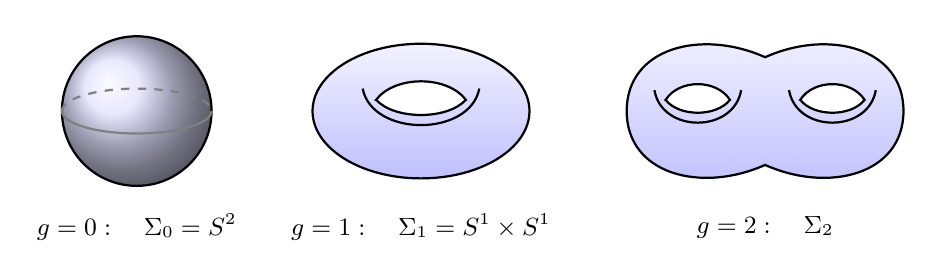
\begin{tikzpicture}[
  scale=0.95,
  line width=0.8pt,
  every node/.style={font=\small}
]

% g=0：球面
\begin{scope}
  \shade[ball color=blue!12] (0,0) circle (1);
  \draw (0,0) circle (1);

  % 赤道：手前は実線, 奥は破線
  \draw[dashed,gray]
    (-1,0) arc[start angle=180,end angle=0,
              x radius=1,y radius=0.3];
  \draw[gray]
    (-1,0) arc[start angle=180,end angle=360,
              x radius=1,y radius=0.3];

  \node at (0,-1.55) {$g=0:\quad \Sigma_0=S^2$};
\end{scope}

% g=1：トーラス
\begin{scope}[shift={(3.8,0)}]
  \shade[top color=blue!5,bottom color=blue!25]
    (0,0) ellipse[x radius=1.45,y radius=0.9];
  \draw (0,0) ellipse[x radius=1.45,y radius=0.9];

  % 穴
  \filldraw[fill=white]
    (-0.6,0.15)
    .. controls (-0.35,0.48) and (0.35,0.48) .. (0.6,0.15)
    .. controls (0.35,-0.12) and (-0.35,-0.12) .. cycle;

  % 穴の手前の曲面
  \draw
    (-0.78,0.30)
    .. controls (-0.65,-0.35) and (0.65,-0.35) .. (0.78,0.30);

  \node at (0,-1.55)
    {$g=1:\quad \Sigma_1=S^1\times S^1$};
\end{scope}

% g=2：二つの取っ手をもつ曲面
\begin{scope}[shift={(8.4,0)}]
  \shade[top color=blue!5,bottom color=blue!25]
    (-1.85,0)
    .. controls (-1.85,0.85) and (-0.85,1.10) .. (0,0.72)
    .. controls (0.85,1.10) and (1.85,0.85) .. (1.85,0)
    .. controls (1.85,-0.85) and (0.85,-1.10) .. (0,-0.72)
    .. controls (-0.85,-1.10) and (-1.85,-0.85) .. cycle;

  \draw
    (-1.85,0)
    .. controls (-1.85,0.85) and (-0.85,1.10) .. (0,0.72)
    .. controls (0.85,1.10) and (1.85,0.85) .. (1.85,0)
    .. controls (1.85,-0.85) and (0.85,-1.10) .. (0,-0.72)
    .. controls (-0.85,-1.10) and (-1.85,-0.85) .. cycle;

  % 二つの穴
  \foreach \a in {-0.9,0.9}{
    \begin{scope}[shift={(\a,0)}]
      \filldraw[fill=white]
        (-0.43,0.15)
        .. controls (-0.25,0.43) and (0.25,0.43) .. (0.43,0.15)
        .. controls (0.25,-0.08) and (-0.25,-0.08) .. cycle;

      \draw
        (-0.58,0.28)
        .. controls (-0.48,-0.30) and (0.48,-0.30) .. (0.58,0.28);
    \end{scope}
  }

  \node at (0,-1.55) {$g=2:\quad \Sigma_2$};
\end{scope}

\end{tikzpicture}
\end{figure}

\begin{exa}\label{O-M245}
補題\ref{exa-cohomology-sphere}より$g(\C\mathbb P^1)=0$である.
\end{exa}

この定理はとても大変なので証明しない. 
定理 \ref{O-M242} には, 例えば次の証明方法がある.\footnote{1つ目は最近勉強したので知っていた. この方法を使うともっとより良いことがわかる. (小林昭七 複素幾何の6章を参照.) 2つ目は知らなかった. 多分小木曽先生の教科書の方法は2つ目になると思う. 2つ目は特異点がを許したコンパクト複素空間上の連接層にも適用できる.なお代数幾何学で示すなら$\C\mathbb P^n$に埋め込んで示す. }
ここでは方針だけを紹介する.

\begin{enumerate}
\item

Dolbeaultの定理とHodge理論を使う方法.
$X$ にHermite計量を入れる.
Dolbeaultの定理とHodge理論により, 
$H^1(X,\mathcal O_X)$ の各類は, 
一意な調和 $(0,1)$ 形式で代表される.
従って, 
\[
H^1(X,\mathcal O_X)
\simeq
\ker\bigl(
\Box_{\bar\partial}:A_X^{0,1}(X)\to A_X^{0,1}(X)
\bigr),
\]
ただし
\[
\Box_{\bar\partial}
=\bar\partial\bar\partial^*
+\bar\partial^*\bar\partial
\]
である.ここで $\bar\partial^*$ は, 
計量から定まる $\bar\partial$ の形式的随伴である.
$\Box_{\bar\partial}$ は楕円型微分作用素であり, 
コンパクト多様体上ではその核が有限次元になる.
これより結論を得る.\footnote{気になる人は私が最近書いたノート"Yauの定理とその応用"の2章を見てほしい. Sobolev空間を用いた楕円型微分作用素の正則性定理を認めれば, あとは結構簡単にわかる. ただ正則性定理が解析をゴリゴリするので難しい. }

\item

ここでは各コチェイン空間に広義一様収束の Fr\'echet 位相を入れる. 以下は Schwartz の有限次元性定理を複体に適用する証明の概略である.

$X$ の有限Leray被覆
\[
\mathcal U=\{U_i\},\qquad
\mathcal V=\{V_i\},\qquad
\overline{V_i}\subset U_i
\]
を選ぶ.どちらも $X$ 全体を覆うものとする.

Montelの定理により, 各次数の制限写像
\[
r^q:C^q(\mathcal U,\mathcal O_X)
\longrightarrow C^q(\mathcal V,\mathcal O_X)
\]
はコンパクトである. 実際, 有限個の共通部分について,
$\overline{V_{i_0}\cap\cdots\cap V_{i_q}}\subset U_{i_0}\cap\cdots\cap U_{i_q}$
となるため, 少し大きいコンパクト集合上で一様に有界な族の制限に Montel の定理を使える.
一方, 定理\ref{O-M229}により両被覆は同じ層コホモロジーを計算するので, 
誘導される写像
\[
\check H^1(\mathcal U,\mathcal O_X)
\xrightarrow[\sim]{\,\check H^1(r)\,}
\check H^1(\mathcal V,\mathcal O_X)
\]
は同型であり, 両辺は $H^1(X,\mathcal O_X)$ と同型である.

ここで, Schwartzの有限次元性定理
\[
\begin{gathered}
\text{フレシェ空間の複体間の写像が各次数でコンパクト}
+
\text{コホモロジー上の写像が全射}
\\[2pt]
\Longrightarrow
\text{送り先のコホモロジーは有限次元}
\end{gathered}
\]
を用いると, 
\[
\dim_{\C}H^1(X,\mathcal O_X)<\infty
\]
を得る.
\end{enumerate}


% SOURCE O:8614 | O-S047 6.2 \quad Riemann--Roch の定理とその最初の応用
\subsection{Riemann--Roch の定理}\label{O-S047}

本節では, コンパクトRiemann 面上の有理型関数を調べる
基本定理であるRiemann--Rochの定理を示す.
以下, 断りがなければ$X$ を種数 $g$ のコンパクトRiemann 面とする.

% SOURCE O:8618 | O-M268
\begin{thm}[Riemann--Rochの定理]\label{O-M268}
$D$ を $X$ 上の因子とする.
このとき, 
\[
h^q(\mathcal O_X(D))
:=\dim_{\C}H^q(X,\mathcal O_X(D))
\qquad(q=0,1)
\]
はともに有限であり, 
\[
h^0(\mathcal O_X(D))-h^1(\mathcal O_X(D))
=\deg D+1-g
\]
が成り立つ.
\end{thm}

ここで $H^0(X,\mathcal O_X(D))$ は, 
$D$ が指定する零点と極の条件を満たす
大域的有理型関数の空間である.
従って, この定理は, その空間の次元を
$h^1(\mathcal O_X(D))$ と結び付けるものである.

\begin{dfn}[Euler--Poincaré標数]\label{O-M269}
\[
\chi(\mathcal O_X(D))
:=h^0(\mathcal O_X(D))-h^1(\mathcal O_X(D))
\]
を $\mathcal O_X(D)$ のEuler--Poincaré標数という.
\end{dfn}

\begin{rem}
$X$ 上の正則関数は定数のみであり, 
$h^1(\mathcal O_X)=g$ だから, 
\[
\chi(\mathcal O_X)=1-g
\]
である.従って, Riemann--Rochの定理は
\[
\chi(\mathcal O_X(D))
=\chi(\mathcal O_X)+\deg D
\]
と書ける.

\end{rem}
以下Riemann--Rochの定理\ref{O-M268}を示そう. 
まずは簡単にわかる線形代数の補題を示す. 

% SOURCE O:8660 | O-M270
\begin{lem}[完全系列と次元の交代和]\label{O-M270}
有限次元線形空間の完全系列
\[
0\longrightarrow V_1\xrightarrow{f_1}V_2
\longrightarrow\cdots
\xrightarrow{f_{n-1}}V_n\longrightarrow0
\]
に対して, 
\[
\sum_{i=1}^n(-1)^i\dim_{\C}V_i=0
\]
が成り立つ.
\end{lem}

\begin{proof}
両端の零写像を $f_0:0\to V_1$, $f_n:V_n\to0$ と書く.
完全性から $\ker f_i=\operatorname{Im}f_{i-1}$ なので, 
各 $i$ に対して短完全系列
\[
0\longrightarrow \ker f_i=\operatorname{Im}f_{i-1}
\longrightarrow V_i
\xrightarrow{f_i}\operatorname{Im}f_i
\longrightarrow0
\]
が得られる.ここで, 最初の写像は包含写像である.

短完全系列では中央の次元が両端の次元の和に等しいので, 
\[
\dim V_i
=\dim\operatorname{Im}f_{i-1}
+\dim\operatorname{Im}f_i
\]
となる.従って, 
\[
\begin{aligned}
\sum_{i=1}^n(-1)^i\dim V_i
&=\sum_{i=1}^n(-1)^i
\left(
\dim\operatorname{Im}f_{i-1}
+\dim\operatorname{Im}f_i
\right)
=0.
\end{aligned}
\]
\end{proof}


\begin{proof}[定理\ref{O-M268}の証明]
零因子から出発し, 一点を加えると $\chi$ が $1$ 増え,
一点を引くと $1$ 減ることを示す.

\medskip
\noindent
\textbf{(1) $D=0$ の場合.}

\[
h^0(\mathcal O_X)
\underalign{\text{(系\ref{O-M067})}}{=}1,
\qquad
h^1(\mathcal O_X)
\underalign{\text{(定理\ref{O-M244})}}{=}g<\infty.
\]
従って, 両群は有限次元であり,
\[
\chi(\mathcal O_X)
=\underbrace{h^0(\mathcal O_X)}_{=1}
-\underbrace{h^1(\mathcal O_X)}_{=g}
=1-g
\]
となる.

\medskip
\noindent
\textbf{(2) 一点を加えると $\chi$ は $1$ 増える.}

補題\ref{O-M210}の短完全系列
\[
0\longrightarrow\mathcal O_X(D)
\longrightarrow\mathcal O_X(D+p)
\longrightarrow\C_p
\longrightarrow0
\]
に, 定理\ref{O-M234}の長完全系列を適用する.
補題\ref{O-M237}より
$H^0(X,\C_p)=\C$, $H^1(X,\C_p)=0$ なので,
\begin{equation}\label{O-EQ068}
\begin{aligned}
0&\longrightarrow H^0(X,\mathcal O_X(D))
\longrightarrow H^0(X,\mathcal O_X(D+p))
\longrightarrow\C\\
&\longrightarrow H^1(X,\mathcal O_X(D))
\longrightarrow H^1(X,\mathcal O_X(D+p))
\longrightarrow0
\end{aligned}
\end{equation}
は完全である.

この完全系列では,
$H^0(X,\mathcal O_X(D))$ は
$H^0(X,\mathcal O_X(D+p))$ の部分空間で,
その商の次元は高々 $1$ である.
また,
$H^1(X,\mathcal O_X(D))\to H^1(X,\mathcal O_X(D+p))$
は全射で, その核の次元は高々 $1$ である.
従って, $D$ と $D+p$ のどちらかで両群が有限次元ならば,
もう一方でも両群は有限次元となる.

このとき, 完全系列の次元の交代和は零なので,
\[
\begin{aligned}
0
&\underalign{\text{(補題\ref{O-M270}, 式\eqref{O-EQ068})}}{=}
h^0(\mathcal O_X(D))-h^0(\mathcal O_X(D+p))+1 -h^1(\mathcal O_X(D))+h^1(\mathcal O_X(D+p))\\
&=
\underbrace{h^0(\mathcal O_X(D))-h^1(\mathcal O_X(D))}
_{\chi(\mathcal O_X(D))}
-
\underbrace{h^0(\mathcal O_X(D+p))-h^1(\mathcal O_X(D+p))}
_{\chi(\mathcal O_X(D+p))}
+1.
\end{aligned}
\]
従って,
\begin{equation}\label{O-EQ069}
\chi(\mathcal O_X(D+p))=\chi(\mathcal O_X(D))+1.
\end{equation}
$D$ を $D-p$ に置き換えれば,
$\chi(\mathcal O_X(D-p))=\chi(\mathcal O_X(D))-1$
も得られる.

\medskip
\noindent
\textbf{(3) 一点ずつ加減して, 一般の因子に進む.}

任意の因子は, 同じ点の繰り返しを許して
\[
D=p_1+\cdots+p_r-q_1-\cdots-q_s
\]
と書ける.
零因子から $p_i$ を一点ずつ加え, $q_j$ を一点ずつ引くと,
(1), (2) より各段階で両群の有限次元性が保たれる.
さらに,
\[
\chi(\mathcal O_X(D))
\underalign{\text{\eqref{O-EQ069}}}{=}
\underbrace{\chi(\mathcal O_X)}_{=1-g}
+\underbrace{r-s}_{=\deg D}
=1-g+\deg D.
\]
これで有限次元性と求める等式が示された.
\end{proof}


$h^1(\mathcal O_X(D))\geq 0$ だから定理 \ref{O-M268} を用いると次を得る. 
% SOURCE O:8804 | O-M271 cor 6.26; original option: 系 6.26, Riemann--Rochの不等式
\begin{cor}[Riemann--Rochの不等式]\label{O-M271}
$X$ の因子 $D$ に対して
\[
h^0(\mathcal O_X(D))\geq 1-g+\deg D.
\]
\end{cor}

\begin{lem}[一点で条件を加えたときの次元の変化]\label{O-M272}
$X$ をコンパクトRiemann 面, $D$ を $X$ 上の因子とする.
このとき, 任意の $p\in X$ に対して
\[
h^0(\mathcal O_X(D))-1
\leq h^0(\mathcal O_X(D-p))
\leq h^0(\mathcal O_X(D))
\]
が成り立つ.
つまり, 因子から一点を引くと, 
大域切断の空間の次元は $1$ 減るか, 変わらない.

従って, $p_1,\ldots,p_n\in X$ に対して
\[
h^0(\mathcal O_X(D-p_1-\cdots-p_n))
\geq h^0(\mathcal O_X(D))-n
\]
である.ここで, 同じ点が繰り返し現れてもよい.
\end{lem}

\begin{proof}
定理\ref{O-M268}の証明で用いた完全系列\eqref{O-EQ068}の最初の三項を, $D$ を $D-p$ に置き換えて使う.

補題 \ref{O-M210} より, 短完全系列
\[
0\longrightarrow\mathcal O_X(D-p)
\longrightarrow\mathcal O_X(D)
\xrightarrow{\rho}\C_p
\longrightarrow0
\]
がある.
大域切断を取ると, 補題 \ref{O-M213} より
\[
0\longrightarrow H^0(X,\mathcal O_X(D-p))
\longrightarrow H^0(X,\mathcal O_X(D))
\xrightarrow{\rho(X)}\C
\]
は完全である.従って, 
\[
h^0(\mathcal O_X(D))
-h^0(\mathcal O_X(D-p))
=\dim_{\C}\operatorname{Im}\rho(X)
\in\{0,1\}.
\]
これで最初の主張を得る.

次に, $p_1,\ldots,p_n$ を一点ずつ引く.
各段階で次元は高々 $1$ しか減らないので, 
全体でも高々 $n$ しか減らない.
従って, 二つ目の不等式も成り立つ.
\end{proof}


% SOURCE O:8832 | O-S048 6.2.1 応用 1：定数ではない大域的有理型関数の存在
\subsection{標準因子}
\label{O-S048}\label{O-S049}


以下断りがなければ $X$ を種数 $g$ のコンパクトRiemann 面とする.
Riemann--Rochの定理を使うと, 
具体的な式を与えなくても, 定数でない有理型関数の存在を示せる.

\begin{thm}[点を区別する有理型関数]\label{O-M273}
$X$ を種数 $g$ のコンパクトRiemann 面とする.
任意の点 $p\in X$ に対して,
$p$ を唯一の極とし, その位数が高々 $g+1$ である
大域的有理型関数 $f$ が存在する.

従って, 異なる二点 $p,q$ に対して,
\[
f(p)=\infty,\qquad f(q)\in\C
\]
となる有理型関数を取れる.
特に, $X$ から $\C\mathbb P^1$ への
全射正則写像が存在する.
\end{thm}

\begin{proof}
$p$ だけに極を許した関数を集め,
その中に定数でない関数があることを示す.

$D=(g+1)p$ とおく.
定義\ref{O-M199}より,
\[
H^0(X,\mathcal O_X(D))
=
\left\{
f\in\mathcal M(X)\ \middle|\
\begin{array}{l}
p\text{ 以外では正則であり,}\\
p\text{ での極は高々 }g+1\text{ 位}
\end{array}
\right\}.
\]
この空間には定数関数も含まれる.
一方, Riemann--Rochの不等式（系\ref{O-M271}）より,
\[
\dim_{\C}H^0(X,\mathcal O_X(D))
\geq
\underbrace{\deg D}_{g+1}+1-g
=2.
\]
定数関数は $1$ の定数倍だけなので,
それらのなす空間は一次元である.
従って, 上の空間には定数でない関数 $f$ が存在する.

この $f$ の極は $p$ にしか現れない.
もし $p$ にも極がなければ, $f$ は $X$ 全体で正則となり,
系\ref{O-M067}より定数になってしまう.
従って, $p$ は実際に極であり,
その位数は高々 $g+1$ である.

よって, $q\neq p$ ならば
$f(p)=\infty$ かつ $f(q)\in\C$ となり,
二点を区別できる.
また, 定理\ref{O-M057}より $f$ は正則写像
$X\to\C\mathbb P^1$ を定め,
定値でないので定理\ref{O-M066}より全射である.
\end{proof}

\begin{thm}[大域的有理型 $1$ 形式の存在]\label{O-M281}
$X$ 上には, 零でない大域的有理型 $1$ 形式が存在する.
\end{thm}

\begin{proof}
定理 \ref{O-M273} より, 
定数でない大域的有理型関数 $f$ が存在する.
その微分 $df$ は, 大域的有理型 $1$ 形式である.
実際, 局所座標 $z$ を用いれば
\[
df=f'(z)\,dz
\]
であり, 有理型関数の導関数も有理型である.

また, $df=0$ ならば $f$ は局所的に定数となり, 
$X$ の連結性から定数になる.
これは $f$ の選び方に反するので, $df\neq0$ である.
\end{proof}

次に, 二つの有理型 $1$ 形式の違いを調べる.
局所的には, どちらも $dz$ の有理型関数倍なので, 
その比は有理型関数になる.

\begin{prop}[二つの有理型 $1$ 形式の比]\label{O-M282}

$\omega_1,\omega_2$ を零でない大域的有理型 $1$ 形式とする.
このとき, 一意な $\varphi\in\mathcal M(X)\setminus\{0\}$ によって $\omega_2=\varphi\omega_1$ と書け, 
\begin{equation}\label{O-EQ077}
\operatorname{div}(\omega_2)
=\operatorname{div}(\omega_1)+\operatorname{div}(\varphi)
\end{equation}
が成り立つ.
\end{prop}
\begin{proof}
局所座標 $z$ を用いて, 二つの形式を
\[
\omega_1=f_z\,dz,\qquad \omega_2=g_z\,dz
\]
と書く.
同じ $dz$ を用いているので,
\[
\omega_2=\frac{g_z}{f_z}\,\omega_1
\]
である.
従って, 求める $\varphi$ は局所的には $g_z/f_z$ である.
$f_z$ の零点でも, 極を許せばこの比は有理型関数として定まる.

この比が別の座標でも同じになることを確認する.
座標 $w$ を使うと,
\[
\omega_1=f_z\frac{dz}{dw}\,dw,\qquad
\omega_2=g_z\frac{dz}{dw}\,dw
\]
なので, 係数の比は
\[
\frac{g_z(dz/dw)}{f_z(dz/dw)}
=\frac{g_z}{f_z}
\]
となる.
つまり, 座標を変えると両方の係数に同じ因子が掛かるため,
比は変わらない.

従って, 各座標近傍で作った比は共通部分で一致し,
大域的有理型関数 $\varphi$ に貼りあわさる.
また, $\omega_2=\varphi\omega_1$ ならば
各座標近傍で必ず $\varphi=g_z/f_z$ となるので,
$\varphi$ は一意である.

最後に, $g_z=\varphi f_z$ より, 各点 $p$ で
\[
\begin{aligned}
\operatorname{ord}_p(\omega_2)
=\operatorname{ord}_p(g_z)
=\operatorname{ord}_p(\varphi)+\operatorname{ord}_p(f_z)=\operatorname{ord}_p(\varphi)+\operatorname{ord}_p(\omega_1).
\end{aligned}
\]
これを各点の係数として並べれば,
因子の等式 \eqref{O-EQ077} を得る.
\end{proof}

\begin{dfn}[因子の線形同値]\label{O-M283}
二つの因子 $D_1,D_2$ に対して, 
ある $f\in\mathcal M(X)\setminus\{0\}$ が存在して
\[
D_2=D_1+\operatorname{div}(f)
\]
となるとき, $D_1,D_2$ は線形同値であるといい, 
\[
D_1\sim D_2
\]
と書く.
つまり, 差が大域的有理型関数の因子となることをいう.
これは因子全体の集合上の同値関係である.
\end{dfn}


\begin{lem}[線形同値な因子]\label{O-M284}
$D_1\sim D_2$ ならば,
\[
\deg D_1=\deg D_2,\qquad \mathcal O_X(D_1)\simeq\mathcal O_X(D_2)
\]
である.
\end{lem}
\begin{proof}
$D_2=D_1+\operatorname{div}(f)$ とする.
補題 \ref{O-M198} より $\deg\operatorname{div}(f)=0$ なので, 
$\deg D_1=\deg D_2$ である.

また, 各開集合 $U$ 上で, $f$ を掛ける写像
\[
\mathcal O_X(D_2)(U)\longrightarrow\mathcal O_X(D_1)(U),
\qquad s\longmapsto fs
\]
を考える.
\[
\operatorname{div}(fs)+D_1
=\operatorname{div}(s)+D_2
\]
だから, この写像は矛盾なく定まり, 
逆写像は $f$ で割る写像である.
制限とも両立するので, 層の同型を得る.

\end{proof}

命題 \ref{O-M282} より, 
零でない有理型 $1$ 形式の因子は, 
どの形式を選んでも互いに線形同値である.

\begin{dfn}[標準因子]\label{O-M285}
零でない大域的有理型 $1$ 形式 $\omega$ を選び, 
\[
K_X:=\operatorname{div}(\omega)
\]
とおく.このような因子を $X$ の標準因子という.
\end{dfn}
標準因子そのものは $\omega$ の選び方に依存するが, 
その線形同値類は $X$ だけで決まる.

\begin{exa}[$\C\mathbb P^1$ の標準因子]\label{exa-canonical-sphere}
定義\ref{O-M093}の位数を用いて, 定義\ref{O-M285}の標準因子を計算する.

$\C\mathbb P^1$ 上の有理型 $1$ 形式 $\omega=dz$ を考える.
有限の点では零点も極もなく, 
無限遠点の局所座標 $w=1/z$ では
\[
dz=-w^{-2}\,dw
\]
となる.従って, 標準因子として
\[
K_{\C\mathbb P^1}=\operatorname{div}(dz)=-2[\infty]
\]
を選べる.

一方, $\omega'=z\,dz$ を選ぶと, 
$0$ に単純零点をもち, 無限遠点では
\[
z\,dz=-w^{-3}\,dw
\]
となるので, 
\[
K'_{\C\mathbb P^1}
=\operatorname{div}(z\,dz)=[0]-3[\infty]
\]
を得る.

この二つは異なる因子だが, 
\[
K'_{\C\mathbb P^1}-K_{\C\mathbb P^1}
=[0]-[\infty]=\operatorname{div}(z)
\]
なので, 線形同値である.
このように, 標準因子の表示は選ぶ形式に依存するが, 
その線形同値類は変わらない.
\end{exa}

\begin{exa}[楕円曲線の標準因子]\label{exa-canonical-torus}
\ref{O-S027}節で構成した複素トーラスについて, 定義\ref{O-M285}を適用する.

楕円曲線 $E=\C/\Lambda$ を考える.
$\C$ 上の正則 $1$ 形式 $dz$ は, 平行移動に対して
\[
d(z+\lambda)=dz\qquad(\lambda\in\Lambda)
\]
を満たすので, $E$ 上の正則 $1$ 形式に降下する.
これも $dz$ と書く.

商写像から得られる局所座標では, その係数は常に $1$ である.
従って, 零点も極もなく, 標準因子として
\[
K_E=\operatorname{div}(dz)=0
\]
を選べる.特に, 
\[
\deg K_E=0,\qquad
\Omega_E^1\simeq\mathcal O_E
\]
である.この同型は $f\mapsto f\,dz$ で与えられる.
\end{exa}

\begin{lem}[標準因子と正則 $1$ 形式の層]\label{O-M286}
零でない大域的有理型 $1$ 形式 $\omega$ を選び,
$K_X=\operatorname{div}(\omega)$ とする.
このとき, $\omega$ を掛ける対応
\[
\mathcal O_X(K_X)\xrightarrow{\sim}\Omega_X^1,
\qquad f\longmapsto f\omega
\]
は $\mathcal O_X$-加群の層の同型である.

すなわち, 各開集合 $U$ 上の正則 $1$ 形式は,
$f\in\mathcal O_X(K_X)(U)$ を用いて
一意に $f\omega$ と書ける.
\end{lem}

\begin{proof}
まず, $\mathcal O_X(K_X)(U)$ の条件を確認する.
$K_X=\sum_p n_p p$ と書けば,
$n_p=\operatorname{ord}_p(\omega)$ である.
定義\ref{O-M199}より,
\[
f\in\mathcal O_X(K_X)(U)
\quad\Longleftrightarrow\quad
\operatorname{ord}_p(f)+n_p\geq0
\quad\text{がすべての }p\in U\text{ で成り立つ}.
\]
一方, 掛け算では位数が加わるので,
\[
\operatorname{ord}_p(f\omega)
=\operatorname{ord}_p(f)+\operatorname{ord}_p(\omega)
=\operatorname{ord}_p(f)+n_p.
\]
従って, 上の条件は $f\omega$ がどの点でも極をもたないこと,
すなわち正則であることに等しい.
零の場合も, 位数を $+\infty$ として同じことが成り立つ.

逆に, $\eta\in\Omega_X^1(U)$ を取る.
命題\ref{O-M282}の証明と同様に, 比
\[
f:=\frac{\eta}{\omega}
\]
は $U$ 上の有理型関数となる.
具体的には, 局所座標で $\omega=h\,dz$, $\eta=k\,dz$
と書いたときの比 $k/h$ であり, 座標の選び方によらない.

$f\omega=\eta$ は正則なので,
先ほどの同値関係から $f\in\mathcal O_X(K_X)(U)$ である.
また, $f\omega=\eta$ ならば必ず $f=\eta/\omega$ となるため,
この表示は一意である.

以上より, 各 $U$ 上で全単射を得る.
この対応は正則関数倍を保ち,
\[
(f\omega)|_V=f|_V\,\omega|_V
\qquad(V\subset U)
\]
と制限にも両立するので,
$\mathcal O_X$-加群の層の同型である.
\end{proof}

% SOURCE O:9330 | O-S050 6.3 Serreの双対定理とその証明
\subsection{Serreの双対定理}\label{O-S050}
本節では, Serreの双対定理を述べ, その証明を与える.\footnote{Serreは1926年生まれで現在100歳である. 最近100歳を記念した集会が開催された. またDolbeaultも1924年生まれで2015年に亡くなり, 90歳まで生きた.}
以下, $X$ を種数 $g$ のコンパクトRiemann 面とする.

Riemann--Rochの定理には
$h^1(\mathcal O_X(D))$ が現れた.
Serreの双対定理は, この数が
ある条件を満たす大域的有理型 $1$ 形式の空間の次元に等しいことを示す.
より正確には, 
\[
H^1(X,\mathcal O_X(D))^*
\simeq H^0(X,\mathcal O_X(K_X-D))
\]
という双対空間の同型を与える.
ここで $V^*=\operatorname{Hom}_{\C}(V,\C)$ である.


\begin{dfn}[非退化な双線形形式]\label{O-M287}
$V,W$ を有限次元 $\C$-線形空間とする.
写像
\[
\langle\, ,\,\rangle:V\times W\longrightarrow\C
\]
が, それぞれの変数について $\C$-線形であるとき, 
双線形形式という.

さらに, 
\[
\begin{aligned}
\langle v,w\rangle=0\quad(\forall w\in W)
&\Longrightarrow v=0,\\
\langle v,w\rangle=0\quad(\forall v\in V)
&\Longrightarrow w=0
\end{aligned}
\]
が成り立つとき, 非退化であるという.
つまり, 零でない元は, 相手を適切に選べば
零でない値を与える.
\end{dfn}

\begin{prop}[非退化な形式と双対空間]\label{O-M288}
非退化な双線形形式
$\langle\, ,\,\rangle:V\times W\to\C$ があれば, 
\[
V\xrightarrow{\sim}W^*,
\qquad v\longmapsto\bigl(w\mapsto\langle v,w\rangle\bigr)
\]
および
\[
W\xrightarrow{\sim}V^*,
\qquad w\longmapsto\bigl(v\mapsto\langle v,w\rangle\bigr)
\]
が得られる.特に, $\dim V=\dim W$ である.
\end{prop}

\begin{proof}
非退化性から, 二つの写像はいずれも単射である.
従って, 
\[
\dim V\leq\dim W,\qquad \dim W\leq\dim V
\]
となる.よって次元は等しく, 両写像は同型である.
\end{proof}


次に, 留数写像
\(
\operatorname{res}:H^1(X,\Omega_X^1)\longrightarrow\C
\)
を構成する.
そのために, $H^1(X,\Omega_X^1)$ の元を
滑らかな $2$ 形式で表す.

\begin{lem}\label{O-M290}
次の系列は, $\C$-線形空間の層の短完全系列である：
\begin{equation}\label{O-EQ078}
0\longrightarrow\Omega_X^1
\longrightarrow A_X^{1,0}
\xrightarrow{d}A_X^{1,1}
\longrightarrow0.
\end{equation}
ここで $A_X^{1,1}=A_X^2$ である.
\end{lem}

\begin{proof}
定義\ref{O-M209}に従い, 各点で $d$ の核が正則形式の芽に一致し, かつ $d$ が芽の上で全射であることを示す.

局所座標 $z$ を用いると, 
\[
d(f\,dz)
=\frac{\partial f}{\partial\overline z}
\,d\overline z\wedge dz
\]
である.
従って, $d(f\,dz)=0$ となるのは $f$ が正則なときであり, 
$d$ の核は $\Omega_X^1$ である.

また, Dolbeault の補題\ref{O-M239}より, 
任意の滑らかな関数 $h$ に対して, 局所的に
\[
\frac{\partial f}{\partial\overline z}=h
\]
を解ける.
従って, 任意の $2$ 形式
$h\,d\overline z\wedge dz$ は局所的に $d(f\,dz)$ と書ける.
これで完全性が示された.
\end{proof}

補題 \ref{O-M238} より
$H^1(X,A_X^{1,0})=0$ なので, 
\eqref{O-EQ078} の長完全系列から
\[
H^1(X,\Omega_X^1)
\simeq
\frac{A_X^{1,1}(X)}{dA_X^{1,0}(X)}
\]
を得る.
つまり, コホモロジー類は滑らかな $2$ 形式 $\beta$ で表され, 
$\beta$ に $d\gamma$ を加えても同じ類を表す.

\begin{dfn}[留数写像]\label{O-M291}
上の表示を用いて, 
\[
\operatorname{res}:H^1(X,\Omega_X^1)\longrightarrow\C,
\qquad
[\beta]\longmapsto\frac{1}{2\pi i}\int_X\beta
\]
と定める. この写像を留数写像という. 一点での留数 $\operatorname{Res}_p$ とは定義域が異なる. 両者の関係は補題\ref{O-M293}で示す.
\end{dfn}

この定義は代表元によらない.
実際, Stokesの定理と $\partial X=\emptyset$ より, 
\[
\int_X(\beta+d\gamma)-\int_X\beta
=\int_Xd\gamma=0
\]
だからである.
また, 積分の線形性から $\operatorname{res}$ は線形写像である.

以下, $X$ をコンパクトRiemann 面, 
$D=\sum_p n_p p$ を $X$ 上の因子とする.

\begin{dfn}[因子の条件を満たす有理型 $1$ 形式の層]\label{dfn-twisted-differentials}
各開集合 $U\subset X$ に対して, 
\[
\Omega_X^1(-D)(U)
:=
\left\{
\alpha\ \middle|\
\begin{array}{l}
\alpha\text{ は }U\text{ 上の有理型 }1\text{ 形式で, }\\
\operatorname{ord}_p(\alpha)\geq n_p
\quad(p\in U)
\end{array}
\right\}
\]
と定める.
零形式も含め, 局所的に零の場合の位数は $+\infty$ とする.
通常の制限写像によって, 
これは $\mathcal O_X$-加群の層となる.

例えば, $D=p$ ならば, 
$\Omega_X^1(-p)$ は $p$ で零になる正則 $1$ 形式の層である.
\end{dfn}

\begin{prop}[標準因子による表示]\label{prop-twisted-canonical}
零でない大域的有理型 $1$ 形式 $\omega$ を選び, 
$K_X=\operatorname{div}(\omega)$ とする.
このとき, $\omega$ を掛ける写像は層の同型
\[
\mathcal O_X(K_X-D)\xrightarrow{\sim}\Omega_X^1(-D),
\qquad f\longmapsto f\omega
\]
を与える.
\end{prop}

\begin{proof}
補題\ref{O-M286}より, $\omega$ を掛ける写像は
$\mathcal O_X(K_X)\simeq\Omega_X^1$ を与える.
同じ対応で, $D$ の位数条件も一致することを確認する.

$D=\sum_p n_p p$ と書く.
有理型関数 $f$ に対して,
\[
\underbrace{\operatorname{ord}_p(f)+\operatorname{ord}_p(\omega)\geq n_p}
_{\mathcal O_X(K_X-D)\text{ の条件}}
\quad\Longleftrightarrow\quad
\underbrace{\operatorname{ord}_p(f\omega)\geq n_p}
_{\Omega_X^1(-D)\text{ の条件}}.
\]
従って, $f\mapsto f\omega$ は求める層の同型を与える.
逆写像は $\alpha\mapsto\alpha/\omega$ である.
\end{proof}

\begin{dfn}[カップ積とSerreの双対形式]

$\alpha\in H^0(X,\Omega_X^1(-D))$ とする.
掛け算による層の準同型
\[
m_\alpha:\mathcal O_X(D)\longrightarrow\Omega_X^1,
\qquad f\longmapsto f\alpha
\]
を定める.

これが誘導するコホモロジー上の写像を用いて, 
\[
\alpha\cup\beta
:=H^1(X,m_\alpha)(\beta)
\qquad
\bigl(\beta\in H^1(X,\mathcal O_X(D))\bigr)
\]
と定める.
この双線形写像
\[
\cup:
H^0(X,\Omega_X^1(-D))
\times H^1(X,\mathcal O_X(D))
\longrightarrow H^1(X,\Omega_X^1)
\]
をカップ積という.

さらに, 留数写像と合成した双線形形式
\[
\langle\alpha,\beta\rangle
:=\operatorname{res}(\alpha\cup\beta)
\]
をSerreの双対形式という.
$\alpha$ を固定すると, この合成は次の図式で表される.
\[
\begin{tikzcd}[column sep=large]
H^1(X,\mathcal O_X(D))\arrow[r,"{H^1(X,m_\alpha)}"]\arrow[rr,bend right=22,"{\langle\alpha,\cdot\rangle}"']
&H^1(X,\Omega_X^1)\arrow[r,"\operatorname{res}"]&\C
\end{tikzcd}
\]

\end{dfn}
この定義が成り立つことを確認する. 定義\ref{O-M199}と
定義\ref{dfn-twisted-differentials}より, $f\in\mathcal O_X(D)(U)$ に対し
\[
\operatorname{ord}_p(f\alpha)\geq\underbrace{-n_p+n_p}_{=0}=0.
\]
従って $f\alpha$ は正則であり, $m_\alpha$ は制限と両立する層の準同型である.
定理\ref{O-M234}によりコホモロジー上の写像が定まり,
定義\ref{O-M291}の留数写像も代表元によらないため, 双対形式は矛盾なく定まる.


\begin{thm}[Serreの双対定理]\label{O-M292}
Serreの双対形式
\[
H^0(X,\Omega_X^1(-D))
\times H^1(X,\mathcal O_X(D))
\longrightarrow\C,
\qquad
(\alpha,\beta)\longmapsto
\operatorname{res}(\alpha\cup\beta)
\]
は非退化である.

従って, 自然な同型
\[
H^0(X,\Omega_X^1(-D))
\xrightarrow{\sim}H^1(X,\mathcal O_X(D))^*,
\qquad
\alpha\longmapsto
\bigl(\beta\mapsto\langle\alpha,\beta\rangle\bigr)
\]
が得られる.特に, 
\[
h^1(\mathcal O_X(D))
=h^0(\Omega_X^1(-D))
=h^0(\mathcal O_X(K_X-D))
\]
である.
\end{thm}


\begin{exa}

例えば $D=0$ とすると, 
\[
H^0(X,\Omega_X^1)\simeq H^1(X,\mathcal O_X)^*,
\qquad
\dim_{\C}H^0(X,\Omega_X^1)=g
\]
である.
つまり, 種数 $g$ は大域的正則 $1$ 形式の空間の次元でもある.
\end{exa}

\subsection{Serreの双対定理の証明}\label{O-S054}
Serreの双対定理の証明を一応書くが, この証明はRiemann 面にしか通用しない. なのであまり重要でないと思う. なお証明はかなりテクニカルである. \footnote{このような証明は私は知らなかった. なおチェックはかなり甘いので, 注意して読んでほしい. }

以下, $X$ は種数 $g$ のコンパクトRiemann 面とする.
定義 \ref{O-M291} の留数写像を用いて, 
\begin{equation}\label{eq-serre-iota}
\iota_D:
H^0(X,\Omega_X^1(-D))
\longrightarrow H^1(X,\mathcal O_X(D))^*,
\qquad
\iota_D(\alpha)(\beta)
=\operatorname{res}(\alpha\cup\beta)
\end{equation}
とおく.
定理 \ref{O-M292} を示すには, 
この写像が単射かつ全射であることを示せばよい.

証明の中心となるのは, 次の局所的な留数計算である.

\begin{lem}[連結準同型と留数]\label{O-M293}
$X$ をコンパクトRiemann 面, $A\leq B$ を因子とする.
補題\ref{O-M210}による短完全系列
\[
0\longrightarrow\mathcal O_X(A)
\longrightarrow\mathcal O_X(B)
\xrightarrow{\rho}\mathcal S
\longrightarrow0
\]
に対して, 定理\ref{O-M234}による連結準同型を
\[
\delta:H^0(X,\mathcal S)
\longrightarrow H^1(X,\mathcal O_X(A))
\]
とする.

$p\in X$ における $A,B$ の係数をそれぞれ $m,n$ とし,
$m<n$ と仮定する.
$p$ の座標近傍 $U$ を
\[
A|_U=mp,\qquad B|_U=np
\]
となるように取る.
$u$ を, $U\setminus\{p\}$ 上で正則であり,
\[
\operatorname{ord}_p(u)\geq-n
\]
を満たす $U$ 上の有理型関数とする.
$s\in H^0(X,\mathcal S)$ を,
$U$ 上では $\rho(u)$, $X\setminus\{p\}$ 上では零となる切断とする.

このとき, 任意の
$\alpha\in H^0(X,\Omega_X^1(-A))$ に対して,
\begin{equation}\label{eq-serre-local-residue}
\langle\alpha,\delta(s)\rangle
=\operatorname{Res}_p(u\alpha)
\end{equation}
が成り立つ.
\end{lem}


\begin{proof}
\textbf{(1) 連結準同型を\v{C}ech表示で書く.}
$U_0=U$, $U_1=X\setminus{p}$ とおく.
$s$ は $U_0$ 上では $u$, $U_1$ 上では $0$ に持ち上げられる.
従って,
\[
\delta(s)
\underalign{\text{(補足\ref{rem-cech-connecting})}}{=}
[0-u]=[-u].
\]
ここで右辺は, 共通部分上の切断 $-u$ が定める
層コホモロジーの類である.
$\alpha$ を掛けると,
\[
\alpha\delta(s)=[-u\alpha]
\in H^1(X,\Omega_X^1)
\]
となる.

\medskip
\noindent
\textbf{(2) 同じ類を滑らかな $2$ 形式で表す.}
補題\ref{O-M290}の短完全系列
\[
0\longrightarrow\Omega_X^1
\longrightarrow A_X^{1,0}
\xrightarrow{d}A_X^{1,1}
\longrightarrow0
\]
に, 定理\ref{O-M234}の長完全系列と
補題\ref{O-M238}の消滅を用いると,
\[
A_X^{1,1}(X)/dA_X^{1,0}(X)
\xrightarrow{\sim}H^1(X,\Omega_X^1)
\]
を得る.
補足\ref{rem-cech-connecting}により,
この対応は
\[
[\gamma]\longmapsto[(\tau_j-\tau_i)],
\qquad d\tau_i=\gamma|_{U_i}
\]
で与えられる.
従って, $\tau_1-\tau_0=-u\alpha$ となる原始形式を作ればよい.

定理\ref{O-M236}の単位の分割を用いて,
$p$ の近くで $1$ となる $\chi\in C_c^\infty(U)$ を取り,
\[
\tau_0=(1-\chi)u\alpha\quad\text{on }U_0,
\qquad
\tau_1=-\chi u\alpha\quad\text{on }U_1
\]
とおく.
$\tau_0$ は $p$ の近くで零なので滑らかである.
$\tau_1$ は $U$ の外に零で延長する.

共通部分では,
\[
\tau_1-\tau_0
=\underbrace{\bigl(-\chi-(1-\chi)\bigr)}_{=-1}u\alpha
=-u\alpha.
\]
また, $u\alpha$ は共通部分上で正則な $1$ 形式なので,
\[
d\tau_1-d\tau_0
=-d(u\alpha)
\underalign{\text{(正則 $1$ 形式は閉形式)}}{=}0.
\]
従って, $d\tau_0,d\tau_1$ は
大域的な滑らかな $2$ 形式 $\gamma$ に貼りあわさる.

上の対応において,
\[
[\gamma]\longmapsto[\tau_1-\tau_0]
=[-u\alpha]=\alpha\delta(s)
\]
である.
よって, 双対積と留数写像の定義から,
\[
\langle\alpha,\delta(s)\rangle
=\operatorname{res}\bigl(\alpha\delta(s)\bigr)
\underalign{\text{(定義\ref{O-M291})}}{=}
\frac{1}{2\pi i}\int_X\gamma.
\]

\medskip
\noindent
\textbf{(3) 面積分を留数で計算する.}
$p$ を中心とする十分小さい閉円板 $D$ を取り,
その近くで $\chi=1$ となるようにする.
このとき,
\[
\gamma=0\quad\text{on }D,\qquad
\gamma=-d(\chi u\alpha)\quad\text{on }X\setminus\{p\}.
\]
従って,
\[
\begin{aligned}
\int_X\gamma
&\underalign{\text{($\gamma|_D=0$)}}{=}
\int_{X\setminus\operatorname{int}D}\gamma
\underalign{\text{($\gamma=-d(\chi u\alpha)$)}}{=}
-\int_{X\setminus\operatorname{int}D}d(\chi u\alpha)
\underalign{\text{(Greenの定理\ref{O-M120})}}{=}
-\int_{\partial(X\setminus\operatorname{int}D)}\chi u\alpha\\
&\underalign{\text{(境界の向きが逆)}}{=}
\int_{\partial D}\chi u\alpha
\underalign{\text{($\chi|_{\partial D}=1$)}}{=}
\int_{\partial D}u\alpha
\underalign{\text{(留数の積分表示)}}{=}
2\pi i\,\operatorname{Res}_p(u\alpha).
\end{aligned}
\]
これを (2) の式に代入して,
\[
\langle\alpha,\delta(s)\rangle
=\frac{1}{2\pi i}\int_X\gamma
=\operatorname{Res}_p(u\alpha)
\]
を得る.
\end{proof}


\begin{lem}[双対写像の単射性]\label{lem-serre-injectivity}
任意の因子 $D$ に対して, $\iota_D$ は単射である.
ここで $\iota_D$ は\eqref{eq-serre-iota}の写像である.
\end{lem}
\begin{proof}
$\iota_D(\alpha)$ は $\beta\mapsto\langle\alpha,\beta\rangle$
という線形写像である.
従って, $\alpha\neq0$ に対して
\(
\langle\alpha,\beta\rangle=1
\)
となる $\beta$ を一つ作ればよい.

$D$ のサポートと $\alpha$ の零点・極を避けて点 $p$ を選ぶ.
$p$ を中心とする局所座標 $z$ を用いて,
\[
\alpha=f(z)\,dz,\qquad f(0)\neq0
\]
と書く.
$p$ の近くで
\(
u:=\frac{1}{zf(z)}
\)
とおけば, $u$ は $p$ に単純極をもち,
\(
u\alpha=\frac{dz}{z}
\)
となる.

補題\ref{O-M210}の短完全系列
\[
0\longrightarrow\mathcal O_X(D)
\longrightarrow\mathcal O_X(D+p)
\longrightarrow\mathcal S
\longrightarrow0
\]
において, $u$ の剰余類を
$s\in H^0(X,\mathcal S)$ とする.
連結準同型で送った類を
\[
\beta:=\delta(s)\in H^1(X,\mathcal O_X(D))
\]
とおくと,
\[
\iota_D(\alpha)(\beta)
=\langle\alpha,\beta\rangle
\underalign{\text{(補題\ref{O-M293})}}{=}
\operatorname{Res}_p(u\alpha)
=\operatorname{Res}_p\left(\frac{dz}{z}\right)
=1.
\]
従って, $\alpha\neq0$ ならば $\iota_D(\alpha)\neq0$ であり,
$\iota_D$ は単射である.
\end{proof}


全射性の証明には, 次の二つの準備をする.

\begin{lem}[次数が負の因子]\label{O-M294}
$\deg A<0$ ならば
\[
H^0(X,\mathcal O_X(A))=0
\]
である.
\end{lem}

\begin{proof}
零でない切断 $f$ が存在すれば, 
\(
\operatorname{div}(f)+A\geq0
\)
である.これは定義\ref{O-M199}の大域切断の条件である.
ところが, 補題 \ref{O-M198} より
$\deg\operatorname{div}(f)=0$ なので, 
\[
0\leq\deg(\operatorname{div}(f)+A)
=\deg A<0
\]
となり, 矛盾する.
\end{proof}
\begin{lem}[因子の条件を留数で判定する]\label{O-M296}
$A\leq D$ を因子とする.
包含 $\mathcal O_X(A)\hookrightarrow\mathcal O_X(D)$ から,
定理\ref{O-M234}により誘導される写像を
\[
\tau:H^1(X,\mathcal O_X(A))
\longrightarrow H^1(X,\mathcal O_X(D))
\]
とする.
$\alpha\in H^0(X,\Omega_X^1(-A))$ と
線形写像
\[
\lambda:H^1(X,\mathcal O_X(D))\longrightarrow\C
\]
が, すべての $\beta\in H^1(X,\mathcal O_X(A))$ に対して
\[
\iota_A(\alpha)(\beta)
\underalign{\text{(定義\eqref{eq-serre-iota})}}{=}
\langle\alpha,\beta\rangle
=\lambda(\tau(\beta)).
\]
を満たすと仮定する.
\eqref{eq-serre-iota}で定めた双対写像 $\iota_A$ を用いると,
この仮定は次の図式の可換性を意味する.
\begin{center}
\begin{tikzcd}[column sep=large,row sep=large]
H^1(X,\mathcal O_X(A))
\arrow[r,"\tau"]
\arrow[dr,"\iota_A(\alpha)"']
&
H^1(X,\mathcal O_X(D))
\arrow[d,"\lambda"]
\\
&\C
\end{tikzcd}
\end{center}

このとき, $\alpha$ は $D$ の位数条件も満たす.
すなわち, $D=\sum_q m_q q$ と書くと,
$\operatorname{ord}_q(\alpha)\geq m_q$
がすべての$q\in X$
で成り立ち, 
従って
\[
\alpha\in H^0(X,\Omega_X^1(-D))
\]
である.
さらに, $\lambda$ はこの $\alpha$ との双対積に等しい.
すなわち, \eqref{eq-serre-iota}の写像 $\iota_D$ に対して,
\(
\lambda=\iota_D(\alpha)
\)
が成り立つ.
\end{lem}

\begin{proof}
まず $\alpha$ が $D$ の位数条件を満たすことを示し,
その後で $\lambda=\iota_D(\alpha)$ を示す.

\medskip
\noindent
\textbf{(1) $\tau$ の核と全射性を確認する.}

補題\ref{O-M210}の短完全系列
\[
0\longrightarrow\mathcal O_X(A)
\longrightarrow\mathcal O_X(D)
\longrightarrow\mathcal S
\longrightarrow0
\]
に, 定理\ref{O-M234}の長完全系列と
補題\ref{O-M237}の $H^1(X,\mathcal S)=0$ を用いると,
\[
H^0(X,\mathcal S)
\xrightarrow{\delta}H^1(X,\mathcal O_X(A))
\xrightarrow{\tau}H^1(X,\mathcal O_X(D))
\longrightarrow0
\]
は完全である.
従って,
\(
\tau\circ\delta=0
\)
かつ $\tau$は全射
となる.
特に, 仮定より, 任意の $s\in H^0(X,\mathcal S)$ に対して
\[
\langle\alpha,\delta(s)\rangle
\underalign{\text{(仮定)}}{=}
\lambda(\tau(\delta(s)))
\underalign{\text{($\tau\circ\delta=0$)}}{=}0.
\]
以下では, $\alpha$ の位数が不足すると,
この値が $1$ になる $s$ を作れることを示す.

\medskip
\noindent
\textbf{(2) $\alpha$ が $D$ の位数条件を満たすこと.}

ある点 $q$ で位数条件が満たされないと仮定する.
$A,D$ の $q$ での係数をそれぞれ $a,m$ とすると,
\[
a\leq r:=\operatorname{ord}_q(\alpha)<m
\]
である.
最初の不等式は
$\alpha\in H^0(X,\Omega_X^1(-A))$ による.

$q$ を中心とする局所座標 $z$ を取り,
\[
\alpha=z^r h(z)\,dz,\qquad
h\text{ は正則},\quad h(0)\neq0
\]
と書く.
近傍を十分小さくして $h$ が零にならないようにし,
\(
u:=\frac{1}{z^{r+1}h(z)}
\)
とおく.
この選び方により,
\(
u\alpha=\frac{dz}{z}.
\)
また,
\[
\operatorname{ord}_q(u)=-r-1
\underalign{\text{($r<m$ は整数の不等式)}}{\geq}-m
\]
なので, $u$ は $q$ の近くで $\mathcal O_X(D)$ の切断である.

$u$ の剰余類を $q$ にもち,
ほかの点では零となる切断
$s\in H^0(X,\mathcal S)$ を取る.
すると,
\[
\langle\alpha,\delta(s)\rangle
\underalign{\text{(補題\ref{O-M293})}}{=}
\operatorname{Res}_q(u\alpha)
=\operatorname{Res}_q\left(\frac{dz}{z}\right)
=1.
\]
これは (1) で得た
$\langle\alpha,\delta(s)\rangle=0$ に矛盾する.
従って, すべての点で位数条件が満たされ,
\(
\alpha\in H^0(X,\Omega_X^1(-D))
\)
である.

\medskip
\noindent
\textbf{(3) $\lambda=\iota_D(\alpha)$ であること.}

(2) により, $\alpha$ を掛ける写像
$\mathcal O_X(D)\to\Omega_X^1$ が定まる.
$\mathcal O_X(A)$ の切断に対しては,
包含で $\mathcal O_X(D)$ に移してから $\alpha$ を掛けても,
直接 $\alpha$ を掛けても同じである.
定理\ref{O-M234}のコホモロジーの函手性により,
この一致はコホモロジー上でも成り立つ.
従って, 任意の $\beta\in H^1(X,\mathcal O_X(A))$ に対して,
\[
\iota_D(\alpha)(\tau(\beta))
=\iota_A(\alpha)(\beta)
\underalign{\text{(仮定)}}{=}
\lambda(\tau(\beta)).
\]
(1) より $\tau$ は全射なので,
$\tau(\beta)$ は $H^1(X,\mathcal O_X(D))$ のすべての元を動く.
よって,
\(
\iota_D(\alpha)=\lambda
\)
である.
\end{proof}

\begin{proof}[定理\ref{O-M292}の証明]
補題\ref{lem-serre-injectivity}により, $\iota_D$ は単射である.
全射性を示すため,
$0\neq\lambda\in H^1(X,\mathcal O_X(D))^*$ を取り,
$\iota_D(\alpha)=\lambda$ となる微分形式 $\alpha$ を作る.
零汎関数は零形式の像なので, 考えなくてよい.

\medskip
\noindent
\textbf{(1) 何を作れば十分か.}

補題\ref{O-M296}によれば, 最初から
$\alpha\in H^0(X,\Omega_X^1(-D))$ を示す必要はない.
ある因子 $A\leq D$ と
$\alpha\in H^0(X,\Omega_X^1(-A))$ を見つけ,
包含が誘導する写像
\[
\tau:H^1(X,\mathcal O_X(A))
\longrightarrow H^1(X,\mathcal O_X(D))
\]
に対して $\iota_A(\alpha)=\lambda\circ\tau$ を示せばよい.
この等式が成り立てば, 同補題により
$\alpha\in H^0(X,\Omega_X^1(-D))$ かつ
$\iota_D(\alpha)=\lambda$ が従う.

そこで, まず適当な関数 $\varphi\neq0$ と微分形式 $\alpha_n$ を用いて,
$\varphi\lambda$ を $\alpha_n$ との双対積として表す.
その後で $\alpha:=\alpha_n/\varphi$ と置き,
上の条件を確認する.

\medskip
\noindent
\textbf{(2) 次元比較によって $\varphi,\alpha_n$ を見つける.}

点 $p\in X$ を固定し, 正の整数 $n$ に対して $D_n:=D-np$ とおく.
$\varphi\in H^0(X,\mathcal O_X(np))$ を掛ける写像
$\mathcal O_X(D_n)\to\mathcal O_X(D)$ が誘導する
コホモロジー上の写像を $\beta\mapsto\varphi\beta$ と書く.
これを用いて,
\[
f_n:H^0(X,\mathcal O_X(np))
\longrightarrow H^1(X,\mathcal O_X(D_n))^*,
\qquad
\varphi\longmapsto\varphi\lambda,
\qquad
(\varphi\lambda)(\beta):=\lambda(\varphi\beta)
\]
と定める.

$f_n$ は単射である.
実際, $\varphi\neq0$ ならば, 層の写像
$\mathcal O_X(D_n)\xrightarrow{\cdot\varphi}\mathcal O_X(D)$
は単射であり, その余核 $\mathcal S_\varphi$ は摩天楼層である.
局所的に両層を正則関数の層と同一視すると,
零でない正則関数による掛け算となり,
その零点でのみ余核が生じるからである.
定理\ref{O-M234}の長完全系列から,
\[
H^1(X,\mathcal O_X(D_n))
\xrightarrow{\ \cdot\varphi\ }H^1(X,\mathcal O_X(D))
\longrightarrow
\underbrace{H^1(X,\mathcal S_\varphi)}_{\text{補題\ref{O-M237}より }0}
\]
は完全である.
従って $\cdot\varphi$ は全射であり,
$\lambda\neq0$ より $\varphi\lambda\neq0$ となる.

一方, 補題\ref{lem-serre-injectivity}より,
\[
\iota_{D_n}:H^0(X,\Omega_X^1(-D_n))
\longrightarrow H^1(X,\mathcal O_X(D_n))^*
\]
も単射である.
この二つの像が零でない元で交われば,
求める $\varphi,\alpha_n$ が得られる.

零でない大域的有理型 $1$ 形式を選び,
その因子を $K_X$ とする
（定理\ref{O-M281}, 定義\ref{O-M285}参照）.
この形式を掛けることで
$\Omega_X^1(-D_n)\simeq\mathcal O_X(K_X-D_n)$ となる.
従って,
\[
\begin{aligned}
\dim\operatorname{Im}f_n
&=h^0(\mathcal O_X(np))
\underalign{\text{(系\ref{O-M271})}}{\geq}n+1-g,\\
\dim\operatorname{Im}\iota_{D_n}
&=h^0(\mathcal O_X(K_X-D+np))
\underalign{\text{(系\ref{O-M271})}}{\geq}
n+\deg K_X-\deg D+1-g.
\end{aligned}
\]
一方, $n>\deg D$ ならば,
補題\ref{O-M294}より $h^0(\mathcal O_X(D_n))=0$ なので,
\[
\dim H^1(X,\mathcal O_X(D_n))^*
\underalign{\text{(定理\ref{O-M268})}}{=}
\underbrace{h^0(\mathcal O_X(D_n))}_{=0}
-\underbrace{\deg D_n}_{=\deg D-n}-1+g
=n-\deg D+g-1.
\]
よって,
\[
\begin{aligned}
&\dim\operatorname{Im}f_n+\dim\operatorname{Im}\iota_{D_n}
-\dim H^1(X,\mathcal O_X(D_n))^*\\
&\qquad\geq
(n+1-g)+(n+\deg K_X-\deg D+1-g)
-(n-\deg D+g-1)
=n+\deg K_X+3-3g.
\end{aligned}
\]
$n$ を十分大きくすれば右辺は正になる.
二つの部分空間の次元の和が周囲の空間の次元より大きいので,
その共通部分は零ではない.

従って, 零でない
$\varphi\in H^0(X,\mathcal O_X(np))$ と
$\alpha_n\in H^0(X,\Omega_X^1(-D_n))$ で,
\begin{equation}\label{eq-serre-common-element}
\varphi\lambda=\iota_{D_n}(\alpha_n)
\end{equation}
を満たすものが存在する.

\medskip
\noindent
\textbf{(3) $\alpha=\alpha_n/\varphi$ と置き, 補題を適用する.}

$\alpha:=\alpha_n/\varphi$ とおく.
$\varphi$ で割ると極が増える可能性があるので,
まず $\alpha$ が満たす因子の条件を調べる.

$\varphi\in H^0(X,\mathcal O_X(np))$ より,
\[
E:=\operatorname{div}(\varphi)+np\geq0,\qquad
A:=D-E=D_n-\operatorname{div}(\varphi)\leq D.
\]
このとき,
\[
\operatorname{div}(\alpha)
=\underbrace{\operatorname{div}(\alpha_n)}_{\geq D_n}
-\operatorname{div}(\varphi)
\geq D_n-\operatorname{div}(\varphi)=A
\]
なので, $\alpha\in H^0(X,\Omega_X^1(-A))$ である.

また, $\operatorname{div}(v/\varphi)+D_n=\operatorname{div}(v)+A$
より, $\varphi$ で割る写像は層の同型
$\mathcal O_X(A)\xrightarrow{\sim}\mathcal O_X(D_n)$ を与える.
この同型と包含が誘導する写像を, それぞれ
\[
\begin{aligned}
j&:H^1(X,\mathcal O_X(A))
\xrightarrow{\sim}H^1(X,\mathcal O_X(D_n))
\qquad
\tau&:H^1(X,\mathcal O_X(A))
\longrightarrow H^1(X,\mathcal O_X(D))
\end{aligned}
\]
と書く.
$\varphi$ で割ってから掛ければ元に戻るので,
$\varphi j(\beta)=\tau(\beta)$ である.
さらに, 局所切断に対する等式
$\alpha v=\alpha_n(v/\varphi)$ から,
\[
\begin{aligned}
\iota_A(\alpha)(\beta)
&\underalign{\text{(掛け算の両立性)}}{=}
\iota_{D_n}(\alpha_n)(j(\beta))
\underalign{\text{(式\eqref{eq-serre-common-element})}}{=}
(\varphi\lambda)(j(\beta))
\underalign{\text{($\varphi\lambda$ の定義)}}{=}
\lambda(\varphi j(\beta))
\underalign{\text{($\varphi j(\beta)=\tau(\beta)$)}}{=}
\lambda(\tau(\beta)).
\end{aligned}
\]
従って, (1) で述べた補題\ref{O-M296}の仮定が満たされ,
\[
\alpha\in H^0(X,\Omega_X^1(-D)),\qquad
\iota_D(\alpha)=\lambda
\]
を得る.
これで全射性が示され, $\iota_D$ は同型である.

両空間は, Riemann--Rochの定理\ref{O-M268}と
$\Omega_X^1(-D)\simeq\mathcal O_X(K_X-D)$ により有限次元である.
従って双対形式は非退化であり,
\[
h^1(\mathcal O_X(D))
=h^0(\Omega_X^1(-D))
=h^0(\mathcal O_X(K_X-D))
\]
が成り立つ.
\end{proof}




\subsection{消滅定理}\label{O-S055}

以下, $X$ を種数 $g$ のコンパクトRiemann 面とする.
Serreの双対定理を用いると, 
Riemann--Rochの定理を大域切断の次元だけで表せる.

\begin{cor}[Riemann--Rochの定理の別形]\label{O-M297}
任意の因子 $D$ に対して, 
\[
h^0(\mathcal O_X(D))
-h^0(\mathcal O_X(K_X-D))
=1-g+\deg D
\]
が成り立つ.
\end{cor}
\begin{proof}
Riemann--Rochの定理\ref{O-M268}に,
Serreの双対定理\ref{O-M292}による次元の等式を代入すると,
\[
\deg D+1-g
\underalign{\text{(定理\ref{O-M268})}}{=}
h^0(\mathcal O_X(D))
-\underbrace{h^1(\mathcal O_X(D))}_{
=h^0(\mathcal O_X(K_X-D))\ \text{(定理\ref{O-M292})}}
=h^0(\mathcal O_X(D))-h^0(\mathcal O_X(K_X-D))
\]
となり, 結論を得る.
\end{proof}

この式では, $1$ 次コホモロジーの次元が, 
零点と極に条件を付けた有理型関数の空間の次元に
置き換わっている.


\begin{cor}[正則 $1$ 形式の次元と標準因子の次数]\label{O-M298}
次の等式が成り立つ.
\begin{enumerate}
\item
\[
h^0(\Omega_X^1)=h^0(\mathcal O_X(K_X))=g.
\]
すなわち, 大域的正則 $1$ 形式全体の空間の次元は, 
$X$ の種数に等しい.

\item
\[
\deg K_X=2g-2.
\]
従って, 零でない大域的有理型 $1$ 形式 $\omega$ に対して, 
零点の位数の総和から極の位数の総和を引くと
$2g-2$ になる.
\end{enumerate}
\end{cor}
\begin{proof}
コンパクトRiemann 面上の正則関数は定数なので,
$h^0(\mathcal O_X)=1$ である（系\ref{O-M067}参照）.

系\ref{O-M297}に $D=0$ を代入すると,
\[
\underbrace{h^0(\mathcal O_X)}_{=1}
-h^0(\mathcal O_X(K_X))
=1-g+\underbrace{\deg 0}_{=0}
\]
となり, $h^0(\mathcal O_X(K_X))=g$ を得る.
従って,
\[
h^0(\Omega_X^1)
\underalign{\text{(補題\ref{O-M286})}}{=}
h^0(\mathcal O_X(K_X))=g
\]
であり, (1) が従う.

次に, 系\ref{O-M297}に $D=K_X$ を代入すると,
\begin{equation}\label{O-EQ083}
\underbrace{h^0(\mathcal O_X(K_X))}_{=g}
-\underbrace{h^0(\mathcal O_X)}_{=1}
=1-g+\deg K_X.
\end{equation}
これを整理して $\deg K_X=2g-2$ を得る.
任意の零でない大域的有理型 $1$ 形式 $\omega$ に対して,
$\operatorname{div}(\omega)$ は標準因子なので,
\[
\deg\operatorname{div}(\omega)
\underalign{\text{(定義\ref{O-M285})}}{=}
\deg K_X=2g-2
\]
となる.
\end{proof}


\begin{exa}[複素トーラスの種数]\label{O-M299}
$E=\C/\Lambda$ を $1$ 次元複素トーラスとする.
このとき, 
\(
g(E)=1
\)
である.
\end{exa}

\begin{proof}
$\C$ 上の $dz$ は, $E$ 上のどこでも零にならない
正則 $1$ 形式に降下する.
この形式も $dz$ と書けば, 
\[
K_E=\operatorname{div}(dz)=0
\]
と取れる.
従って,
\[
2g(E)-2
\underalign{\text{(系\ref{O-M298})}}{=}
\deg K_E=0
\]
となり, $g(E)=1$ を得る.
\end{proof}


\begin{exa}[Riemann 球面の種数]\label{O-M300}
Riemann 球面の種数は
\(
g(\C\mathbb P^1)=0
\)
である.
\end{exa}
\begin{proof}
$\C_z$ 上の $dz$ は零点も極ももたない.
無限遠点の局所座標 $w=1/z$ を用いると,
\[
dz=d(w^{-1})=\underbrace{-w^{-2}}_{\text{位数 }-2}\,dw
\]
なので, 無限遠点に $2$ 位の極をもつ.
従って,
\[
K_{\C\mathbb P^1}
\underalign{\text{(定義\ref{O-M285})}}{:=}
\operatorname{div}(dz)=-2[\infty]
\]
と取れる.
よって,
\[
2g(\C\mathbb P^1)-2
\underalign{\text{(系\ref{O-M298})}}{=}
\deg K_{\C\mathbb P^1}=-2
\]
となり, $g(\C\mathbb P^1)=0$ を得る.
\end{proof}



次に, 因子の次数からコホモロジーの消滅を判定する.
基本となるのは, 
「次数が負の因子には, 零でない大域切断が存在しない」
という事実である.

\begin{cor}[消滅定理と次元公式]\label{O-M301}\label{O-M302}
$X$ を種数 $g$ のコンパクトRiemann 面とし, 
$D$ を $X$ 上の因子とする.
\begin{enumerate}
\item
$\deg D<0$ ならば, 
\[
H^0(X,\mathcal O_X(D))=0.
\]

\item
$\deg D\geq2g-1$ ならば, 
\[
H^1(X,\mathcal O_X(D))=0,
\qquad
h^0(\mathcal O_X(D))=\deg D+1-g.
\]
\end{enumerate}
\end{cor}
\begin{proof}
(1) は補題\ref{O-M294}で示した.

(2) について,
\[
\deg(K_X-D)=\deg K_X-\deg D
\underalign{\text{(系\ref{O-M298})}}{=}
2g-2-\deg D
\underalign{\text{(仮定 $\deg D\geq2g-1$)}}{\leq}-1<0.
\]
従って,
\[
h^1(\mathcal O_X(D))
\underalign{\text{(Serreの双対定理\ref{O-M292})}}{=}
h^0(\mathcal O_X(K_X-D))
\underalign{\text{((1))}}{=}0.
\]
これをRiemann--Rochの定理\ref{O-M268}に代入すると,
\[
h^0(\mathcal O_X(D))
\underalign{\text{(定理\ref{O-M268})}}{=}
\deg D+1-g+\underbrace{h^1(\mathcal O_X(D))}_{=0}
=\deg D+1-g.
\]
\end{proof}


\subsection{コンパクトRiemann 面の$3$ 種の神器}
$3$ 種の神器とは古事記・日本書紀など日本の神話に出てくるものである. 重要なので定義しておこう. 
\begin{defn}
$3$ 種の神器とは以下の三つのことである
\begin{itemize}
    \item

    
    八咫鏡（やたのかがみ）
天照大御神が天岩戸に隠れ, 世界が暗闇に包まれた
    「\textbf{天岩戸の神話}」に登場する.
    神々は天照大御神を岩戸の外へ誘い出すため, 
    鏡作りの神である\textbf{伊斯許理度売命
    （いしこりどめのみこと）}に鏡を作らせた.
    
    岩戸の外で神々が宴を開き, 
    天照大御神が何事かと岩戸を少し開けた際, 
    この鏡に映った自分の姿を見せることで
    天照大御神を外へ誘い出したとされる.
    
    その後, 天照大御神は天孫降臨の際に
    この鏡を瓊瓊杵尊（ににぎのみこと）に授け, 
    自分自身を祀るようにこの鏡を祀るよう命じたとされる.
    
    現在は\textbf{伊勢神宮内宮}に祀られているとされる.

    \item

    
    八尺瓊勾玉（やさかにのまがたま）
八咫鏡と同じく「\textbf{天岩戸の神話}」に登場する.
    天照大御神を岩戸から誘い出すため, 
    \textbf{玉祖命（たまのおやのみこと）}が
    多数の勾玉をつないだ玉飾りを作ったとされる.
    
    この勾玉と八咫鏡を榊の枝に掛け, 
    神々が岩戸の前で祭祀を行った.
    
    その後, 天孫降臨の際に八咫鏡・草薙剣とともに
    瓊瓊杵尊に授けられ, 
    三種の神器の一つとなった.
    
    現在は\textbf{皇居・宮中}に安置されているとされる.

    \item

    
    草薙剣（くさなぎのつるぎ）
もともとは
    \textbf{天叢雲剣（あめのむらくものつるぎ）}
    と呼ばれた剣で, 
    「\textbf{須佐之男命による八岐大蛇退治}」の神話に登場する.
    
    須佐之男命（すさのおのみこと）が出雲で
    八岐大蛇（やまたのおろち）を退治し, 
    その尾を切ったところ, 中から立派な剣が現れた.
    須佐之男命はこれを特別な剣であるとして
    天照大御神に献上した.
    
    その後, この剣も天孫降臨の際に
    瓊瓊杵尊へ授けられたとされる.
    
    さらに後の「\textbf{日本武尊（やまとたけるのみこと）}」
    の物語にも登場する.
    日本武尊が東国征討の途中で火攻めに遭った際, 
    この剣で周囲の草を薙ぎ払い, 
    火を切り抜けたという伝承から
    「\textbf{草薙剣}」と呼ばれるようになったとされる.
    
    現在は\textbf{熱田神宮}に祀られているとされる.
\end{itemize}
\end{defn}

神話の時系列で見ると
三種の神器は最初から「三点セット」として登場するわけではない. 
\[
\boxed{
\begin{array}{ccl}
\text{天岩戸} &&
\text{八咫鏡・八尺瓊勾玉が作られる}\\[2mm]
\downarrow &&\\
\text{八岐大蛇退治} &&
\text{天叢雲剣が発見される}\\[2mm]
\downarrow &&\\
\text{天照大御神のもとに三つが集まる}&&\\
\downarrow &&\\
\text{天孫降臨} &&
\text{瓊瓊杵尊に三つが授けられる}
\end{array}}
\]
という構造になっている.
さて, 以下の文章は教科書をそのまま書いた. \footnote{ちなみに私はこれを$3$ 種の神器と呼ぶ人に会ったことはないが, 多分小木曽先生の知り合いにいたのかもしれない. 後藤先生に聞いたらなんかわかるんですかね？？}

% SOURCE O:10254 | O-M303 rem 6.53; original option: 注意 6.53
\begin{tcolorbox}[mybox]
\label{O-M303}
Riemann--Rochの定理, Serreの双対定理, 消滅定理は, 任意次元のコンパクト複素多様体とその因子に対しても適切な形で拡張されていて, 代数幾何学, 複素多様体論の最も基本的な道具になっている. この $3$ つの定理をセットにして $3$ 種の神器と呼ぶ人もいる.
\end{tcolorbox}

ということでまとめておこう. 
% SOURCE O:10258 | O-M304 まとめ 6.54

\begin{thm}[コンパクトRiemann 面の $3$ 種の神器]
\label{O-M-summary}
$X$を種数$g=h^1(\mathcal O_X)$のコンパクトRiemann 面, $D$を$X$の因子とする.
\begin{enumerate}
\item (Riemann--Rochの定理) 
$$ h^0(\mathcal O_X(D))-h^1(\mathcal O_X(D))=1-g+\deg D.$$
\item (Serreの双対定理)$$h^1(\mathcal O_X(D))=h^0(\mathcal O_X(K_X-D)).$$
\item (消滅定理) $\deg D\geq \deg K_X+1=2g-1$ ならば $$h^1(\mathcal O_X(D))=0.$$
\end{enumerate}
\end{thm}

\subsection{Kodaira 消滅定理・Kawamata--Viehweg消滅定理・Nadel消滅定理}

定理\ref{O-M-summary}の三つの結果は, 高次元でも適切な形に一般化される. とりわけ消滅定理は, 特異点を許す場合にも拡張され, 大域切断の構成や極小モデル理論の重要な道具となる. 以下ではその代表例を紹介する.


定理 \ref{O-M-summary} (3) は, Kodaira 消滅定理の一次元版である.
実際, $D$ を
\[
D=K_X+(D-K_X)
\]
と書くと, 系 \ref{O-M298} より
\[
\deg D\geq2g-1
\quad\Longleftrightarrow\quad
\deg(D-K_X)>0
\]
である.従って, 系 \ref{O-M301} (2) は
\[
\deg(D-K_X)>0
\quad\Longrightarrow\quad
H^1\bigl(X,\mathcal O_X(K_X+(D-K_X))\bigr)=0
\]
と書き直せる.
つまり, 標準因子に次数が正の因子を加えると, 
$1$ 次コホモロジーが消滅する.

一般に, Kodaira 消滅定理は, 滑らかな複素射影多様体 $X$ と
豊富な因子 $A$ に対して, 
\[
H^q(X,\mathcal O_X(K_X+A))=0
\qquad(q\geq1)
\]
と主張する.
コンパクトRiemann 面では, 因子 $A$ が豊富であることは
$\deg A>0$ と同値なので, 
$A=D-K_X$ とすれば上の主張に一致する.


Kodaira 消滅定理には, 次のような一般化がある.
ここでは用語の定義には立ち入らず, 主張と応用だけを紹介する.
$X$ を滑らかな複素射影多様体とする.

\begin{enumerate}
\item

Kawamata--Viehweg消滅定理.
因子 $A$ がネフかつ巨大（nef and big）ならば, 
\[
H^q(X,\mathcal O_X(K_X+A))=0
\qquad(q\geq1)
\]
である.
Kodaira 消滅定理の「豊富」という仮定を弱めたものであり, 
極小モデル理論（MMP）における
基点自由化定理などの重要な道具となる.

\item

Nadel消滅定理.
直線束 $\mathcal O_X(A)$ に, 
曲率があるKähler形式 $\omega$ の正の定数倍以上となる
特異Hermite計量 $h$ が存在するとする：
\[
\sqrt{-1}\,\Theta_h\geq\varepsilon\omega,
\qquad \varepsilon>0.
\]
この不等式はカレントの意味で考える.
このとき, 
\[
H^q\bigl(X,\mathcal O_X(K_X+A)\otimes\mathcal I(h)\bigr)=0
\qquad(q\geq1)
\]
である.
ここで $\mathcal I(h)$ は, 
計量の特異性に対応する乗数イデアル層である.

この定理は, 滑らかな正の計量を用いるKodaira 消滅定理を, 
特異な計量に広げたものである.
大域切断の構成や点の分離, 
射影埋め込みの研究などに用いられる.
\end{enumerate}

これらの応用でも, 基本となる考え方は本節と同じである.
すなわち, $H^1$ の消滅によって切断の間の写像を全射にし, 
指定した条件を満たす大域切断を作る.
これを次の章で見ていく. 





\newpage
% SOURCE O:10270 | O-S056 7 Riemann--Rochの定理の応用
\section{Hodge分解・豊富因子・Riemann 面の代数性}\label{O-S056}

この章の前半では, 正則 $1$ 形式と位相的なコホモロジーを結び付ける Hodge 分解を扱う.
後半では, 豊富因子を用いてコンパクトRiemann 面を複素射影空間に埋め込み,
その像が代数曲線であることを示す.

% SOURCE O:10274 | O-S057 7.1 コンパクトRiemann 面の位相的Euler数と種数
\subsection{コンパクトRiemann 面の位相的Euler数と種数}\label{O-S057}
以下 断りがなければ, $X$ は種数 $g$ のコンパクトRiemann 面とする.
これまで, コンパクトRiemann 面 $X$ の種数を
\[
g(X)=\dim_{\C}H^1(X,\mathcal O_X)
\]
と定義してきた.
一方, 曲面の分類定理 \ref{O-M174} によれば, 
$X$ は球面にいくつかの取っ手を付けた曲面と同相である.

本節では, この取っ手の個数が $g(X)$ に等しいことを示す.
まず, 正則写像の次数と分岐から種数を計算する公式を証明する.

\begin{thm}[Hurwitzの公式]\label{O-M306}
$X,Y$ をコンパクトRiemann 面とし,
$f:X\to Y$ を次数 $d$ の定数でない正則写像とする.
$f$ の分岐点を $p_1,\ldots,p_n$,
$p_i$ での分岐指数を $e_i$ とすると,
\[
2g(X)-2
=d\bigl(2g(Y)-2\bigr)+\sum_{i=1}^n(e_i-1)
\]
が成り立つ.
分岐点がない場合, 右辺の和は $0$ とする.
\end{thm}

\begin{proof}
有理型 $1$ 形式の引き戻しの位数を足し合わせ,
標準因子の次数を比較する.

定理\ref{O-M281}により,
$Y$ 上の零でない大域的有理型 $1$ 形式 $\omega$ を取る.
$f$ は定数でないので, $f^*\omega$ も零でない有理型 $1$ 形式である.
従って,
\[
K_Y=\operatorname{div}(\omega),\qquad
K_X=\operatorname{div}(f^*\omega)
\]
と取れる（定義\ref{O-M285}参照）.

各点 $p\in X$ に対して,
\[
\operatorname{ord}_p(f^*\omega)
\underalign{\text{(命題\ref{O-M115})}}{=}
e_p\operatorname{ord}_{f(p)}(\omega)+(e_p-1)
\]
である.
ここで, 分岐しない点では $e_p=1$ とする.

この等式をすべての点について足す.
同じ像 $q\in Y$ をもつ点をまとめると,
\[
\begin{aligned}
\deg K_X
&=\sum_{q\in Y}\sum_{p\in f^{-1}(q)}
\bigl(e_p\operatorname{ord}_q(\omega)+(e_p-1)\bigr)\\
&=\sum_{q\in Y}\operatorname{ord}_q(\omega)
\underbrace{\sum_{p\in f^{-1}(q)}e_p}_{=d\ \text{(定理\ref{O-M071})}}
+\underbrace{\sum_{p\in X}(e_p-1)}_{\text{分岐点以外では }0}
=d\,\deg K_Y+\sum_{i=1}^n(e_i-1).
\end{aligned}
\]
従って,
\begin{equation}\label{O-EQ084}
\deg K_X=d\,\deg K_Y+\sum_{i=1}^n(e_i-1)
\end{equation}
を得る.
最後に,
\[
2g(X)-2
\underalign{\text{(系\ref{O-M298})}}{=}
\deg K_X
\underalign{\text{(式\eqref{O-EQ084})}}{=}
d\,\underbrace{\deg K_Y}_{=2g(Y)-2\ \text{(系\ref{O-M298})}}
+\sum_{i=1}^n(e_i-1)
\]
より, 結論が従う.
\end{proof}


この公式の $\sum_i(e_i-1)$ は, 
分岐によって生じる補正項である.
次に, 同じ補正項が位相的Euler数の計算にも現れることを示す.


\begin{lem}[分岐被覆とEuler数]\label{lem-euler-branched-cover}
$X,Y$ をコンパクトRiemann 面とし,
$f:X\to Y$ を次数 $d$ の定数でない正則写像とする.
$f$ の分岐点を $p_1,\ldots,p_n$,
それぞれの分岐指数を $e_1,\ldots,e_n$ とすると,
\[
\chi_{\mathrm{top}}(X)
=d\,\chi_{\mathrm{top}}(Y)-\sum_{i=1}^n(e_i-1)
\]
が成り立つ.
ここで $\chi_{\mathrm{top}}$ は位相的Euler数であり,
分岐点がない場合, 右辺の和は $0$ とする.
\end{lem}

\begin{proof}
$Y$ の頂点・辺・面の逆像を数えて, $X$ のEuler数を求める.
分岐値を頂点に取ると, 辺と面の個数は $d$ 倍になり,
頂点の個数だけに分岐による補正が入る.

分岐値 $f(p_1),\ldots,f(p_n)$ をすべて頂点に含むように,
$Y$ を三角形分割する.
頂点, 辺, 面の個数をそれぞれ $v,e,t$ とすると,
$\chi_{\mathrm{top}}(Y)=v-e+t$ である.
この分割を $f$ によって $X$ に持ち上げる.
\footnote{
逆像から得られる分割は, セル分割として扱えばよい.
この場合も, 頂点数から辺数を引き, 面数を加えることで
Euler数を計算できる.
}

\medskip
\noindent
\textbf{(1) 辺と面の個数.}

分岐値はすべて頂点にあるので,
辺の内部と面の内部の上では $f$ は不分岐被覆である.
辺の内部は開区間, 面の内部は開円板と同相であり,
どちらも単連結なので, その逆像は $d$ 枚に分かれる.

従って, 各辺・各面に対して $d$ 個ずつ持ち上げがあり,
$X$ 上の辺の個数は $de$, 面の個数は $dt$ である.

\medskip
\noindent
\textbf{(2) 頂点の個数.}

$Y$ の頂点 $q$ を一つ取る.
定理\ref{O-M071}によれば,
逆像を分岐指数の重複度で数えた個数は $d$ である.
しかし, 頂点を数える際には, 各点を一個と数える.
従って,
\[
\#f^{-1}(q)
=\sum_{p\in f^{-1}(q)}1
=\underbrace{\sum_{p\in f^{-1}(q)}e_p}_{=d\ \text{(定理\ref{O-M071})}}
-\sum_{p\in f^{-1}(q)}(e_p-1).
\]
つまり, 分岐指数が $e_p$ の点では,
分岐がない場合に比べて頂点が $e_p-1$ 個少なくなる.

例えば, 次数 $2$ の写像で,
$q$ の逆像に分岐指数 $2$ の点があるとき,
逆像は二点ではなく一点になる.
この様子を局所標準形 $w=z^2$ で表したものが
図\ref{fig-euler-branched-cover}である.

% 図は変更しない.
\begin{figure}[htbp]
\centering
\begin{tikzpicture}[
  scale=1.05,
  every node/.style={font=\small},
  surface/.style={draw=gray!65,dashed},
  face/.style={fill=blue!12,draw=blue!70!black,thick},
  point/.style={circle,fill=black,inner sep=1.5pt}
]

% 左：始域の局所座標円板
\begin{scope}[shift={(-2.7,0)}]
  \node at (0,2.0) {$X$：$p$ の近傍};
  \draw[surface] (0,0) circle (1.5);

  % T の二つの持ち上げ
  \path[face]
    (0,0)--(0:1.5)
    arc[start angle=0,end angle=45,radius=1.5]
    --cycle;
  \path[face]
    (0,0)--(180:1.5)
    arc[start angle=180,end angle=225,radius=1.5]
    --cycle;

  \node[blue!70!black] at (22.5:0.95) {$T_1$};
  \node[blue!70!black] at (202.5:0.95) {$T_2$};

  % 共通の頂点と, 外側の頂点
  \node[point,label=above left:{$p$}] at (0,0) {};
  \foreach \a in {0,45,180,225}
    \node[point] at (\a:1.5) {};

  \node at (0,-2.0) {面は二枚, 中心の頂点は一個};
\end{scope}

% 写像
\draw[-{Stealth},thick]
  (-0.75,0.35)--(0.75,0.35)
  node[midway,above] {$f$};
\node at (0,-0.12) {$w=z^2$};

% 右：終域の局所座標円板
\begin{scope}[shift={(2.7,0)}]
  \node at (0,2.0) {$Y$：$q=f(p)$ の近傍};
  \draw[surface] (0,0) circle (1.5);

  % 分岐値を頂点にもつ面
  \path[face]
    (0,0)--(0:1.5)
    arc[start angle=0,end angle=90,radius=1.5]
    --cycle;

  \node[blue!70!black] at (45:0.95) {$T$};

  \node[point,label=below left:{$q$}] at (0,0) {};
  \foreach \a in {0,90}
    \node[point] at (\a:1.5) {};

  \node at (0,-2.0) {分岐値 $q$ を頂点に取る};
\end{scope}

\end{tikzpicture}
\caption{
分岐指数 $2$ の局所模型.
青い扇形は, 曲線で囲まれた三角形とみなす.
$T$ の内部は二枚に持ち上がるが,
二つの面 $T_1,T_2$ は頂点 $p$ を共有する.
この点での頂点数の補正は $e_p-1=1$ である.
}
\label{fig-euler-branched-cover}
\end{figure}

すべての頂点 $q$ について足し合わせる.
分岐しない点では $e_p-1=0$ なので,
$X$ 上の頂点の個数は
\[
dv-\sum_{i=1}^n(e_i-1)
\]
となる.

\medskip
\noindent
\textbf{(3) Euler数を計算する.}

以上の個数をまとめると,
\[
\begin{array}{c|ccc}
 & \text{頂点} & \text{辺} & \text{面}\\ \hline
Y & v & e & t\\[2pt]
X & dv-\displaystyle\sum_{i=1}^n(e_i-1) & de & dt
\end{array}
\]
である.
従って,
\[
\begin{aligned}
\chi_{\mathrm{top}}(X)
&\underalign{\text{(Euler数の定義)}}{=}
\underbrace{\left(dv-\sum_{i=1}^n(e_i-1)\right)}_{\text{頂点数}}
-\underbrace{de}_{\text{辺数}}+\underbrace{dt}_{\text{面数}}\\
&=d\,\underbrace{(v-e+t)}_{=\chi_{\mathrm{top}}(Y)}
-\sum_{i=1}^n(e_i-1)
=d\,\chi_{\mathrm{top}}(Y)-\sum_{i=1}^n(e_i-1).
\end{aligned}
\]
これで結論を得る.
\end{proof}



\begin{thm}[解析的種数と位相的種数の一致]\label{O-M305}
$X$ をコンパクトRiemann 面とする.
解析的種数
\[
g(X):=\dim_{\C}H^1(X,\mathcal O_X)
\]
は, 位相的種数 $\pi(X)$, すなわち
$X$ の取っ手の個数に等しい：
\[
g(X)=\pi(X)=\frac12 b_1(X).
\]
従って, $X$ は球面に $g(X)$ 個の取っ手を付けた曲面
$\Sigma_{g(X)}$ と同相である
（図 \ref{fig-surfaces-genus}）.
また, 
\[
\chi_{\mathrm{top}}(X)=2-2g(X)=-\deg K_X
\]
が成り立つ.
\end{thm}
% 本文
\begin{figure}[htbp]
\centering
\begin{tikzpicture}[
  scale=0.9,
  line width=0.8pt,
  every node/.style={font=\small}
]
% pi(X)=0：球面
\begin{scope}
  \shade[ball color=blue!12] (0,0) circle (1);
  \draw (0,0) circle (1);
  \draw[dashed,gray]
    (-1,0) arc[start angle=180,end angle=0,
              x radius=1,y radius=0.3];
  \draw[gray]
    (-1,0) arc[start angle=180,end angle=360,
              x radius=1,y radius=0.3];
  \node at (0,-1.5) {$\pi(X)=0$};
  \node at (0,-2.0) {球面 $\Sigma_0$};
\end{scope}
% pi(X)=1：トーラス
\begin{scope}[shift={(3.8,0)}]
  \shade[top color=blue!5,bottom color=blue!25]
    (0,0) ellipse[x radius=1.45,y radius=0.9];
  \draw (0,0) ellipse[x radius=1.45,y radius=0.9];
  % 取っ手の穴
  \filldraw[fill=white]
    (-0.6,0.15)
    .. controls (-0.35,0.48) and (0.35,0.48) .. (0.6,0.15)
    .. controls (0.35,-0.12) and (-0.35,-0.12) .. cycle;
  % 穴の手前の曲面
  \draw
    (-0.78,0.30)
    .. controls (-0.65,-0.35) and (0.65,-0.35) .. (0.78,0.30);
  \node at (0,-1.5) {$\pi(X)=1$};
  \node at (0,-2.0) {取っ手が一個の曲面 $\Sigma_1$};
\end{scope}
% pi(X)=2：二つの取っ手
\begin{scope}[shift={(8.4,0)}]
  \shade[
    top color=blue!5,
    bottom color=blue!25,
    draw=black
  ]
    (-1.85,0)
    .. controls (-1.85,0.85) and (-0.85,1.10) .. (0,0.72)
    .. controls (0.85,1.10) and (1.85,0.85) .. (1.85,0)
    .. controls (1.85,-0.85) and (0.85,-1.10) .. (0,-0.72)
    .. controls (-0.85,-1.10) and (-1.85,-0.85) .. cycle;
  \foreach \a in {-0.9,0.9}{
    \begin{scope}[shift={(\a,0)}]
      \filldraw[fill=white]
        (-0.43,0.15)
        .. controls (-0.25,0.43) and (0.25,0.43) .. (0.43,0.15)
        .. controls (0.25,-0.08) and (-0.25,-0.08) .. cycle;
  \draw
    (-0.58,0.28)
    .. controls (-0.48,-0.30) and (0.48,-0.30) .. (0.58,0.28);
\end{scope}
  }
  \node at (0,-1.5) {$\pi(X)=2$};
  \node at (0,-2.0) {取っ手が二個の曲面 $\Sigma_2$};
\end{scope}
\end{tikzpicture}
\caption{
位相的種数 $\pi(X)$ は取っ手の個数を表す.
図はいずれも境界のない閉曲面の模式図であり,
白い部分は曲面を貫く穴を表す.
}
\label{fig-surfaces-genus}
\end{figure}
\begin{proof}
定理\ref{O-M273}により, 定数でない正則写像
$f:X\to\C\mathbb P^1$ を取る.
その次数を $d$, 分岐点での分岐指数を $e_1,\ldots,e_n$ とする.
このとき,
\[
\begin{aligned}
\chi_{\mathrm{top}}(X)
&\underalign{\text{(補題\ref{lem-euler-branched-cover})}}{=}
d\,\underbrace{\chi_{\mathrm{top}}(\C\mathbb P^1)}_{=2}
-\sum_{i=1}^n(e_i-1)
=2d-\sum_{i=1}^n(e_i-1)\\
&\underalign{\text{(定理\ref{O-M306}, $g(\C\mathbb P^1)=0$)}}{=}
2-2g(X)
\underalign{\text{(系\ref{O-M298})}}{=}
-\deg K_X.
\end{aligned}
\]
ここで $g(\C\mathbb P^1)=0$ は例\ref{O-M300}による.

一方, 曲面の分類定理\ref{O-M174}より,
$X$ は $\Sigma_{\pi(X)}$ と同相であり,
\[
2-2\pi(X)=\chi_{\mathrm{top}}(X)=2-2g(X),
\qquad b_1(X)=2\pi(X).
\]
従って, $g(X)=\pi(X)=\frac12 b_1(X)$ であり,
$X$ は $\Sigma_{g(X)}$ と同相である.
\end{proof}





% SOURCE O:10439 | O-S058 7.2 いろいろなコンパクトRiemann 面の種数
\subsection{いろいろなコンパクトRiemann 面の種数}\label{O-S058}

\begin{exa}[Fermat曲線の種数]\label{O-M310}
例 \ref{O-M170} の $m$ 次Fermat曲線
\[
F_m=\left\{
[X_0:X_1:X_2]\in\C\mathbb P^2
\;\middle|\;
X_0^m+X_1^m+X_2^m=0
\right\}
\qquad(m\geq1)
\]
の種数は
\[
g(F_m)=\frac{(m-1)(m-2)}2
\]
である.
\end{exa}
\begin{proof}
有理型 $1$ 形式 $\omega$ を一つ作り,
その零点・極の位数から $\deg K_{F_m}$ を計算する.
局所座標 $z$ で $\omega=h(z)\,dz$ と書いたとき,
$\omega$ の位数は係数 $h$ の位数である
（定義\ref{O-M093}参照）.

\medskip
\noindent
\textbf{(1) 有限部分では零点も極もない形式を作る.}

$X_0\neq0$ 上で $x=X_1/X_0$, $y=X_2/X_0$ とおく.
曲線の方程式 $1+x^m+y^m=0$ を微分すると,
\[
m x^{m-1}\,dx+m y^{m-1}\,dy=0
\]
となるので,
\[
\omega:=\frac{dx}{m y^{m-1}}
=-\frac{dy}{m x^{m-1}}
\]
という有理型 $1$ 形式が得られる.
分母が零になる点では, もう一方の表示を使えばよい.

実際, $y\neq0$ の点では,
正則陰関数定理\ref{thm-holomorphic-implicit}により
$y$ は $x$ の正則関数として書け, $x$ が局所座標となる.
従って,
\[
\omega=\underbrace{\frac{1}{m y^{m-1}}}_{\text{正則かつ非零}}\,dx
\]
は零点も極ももたない.

一方, $y=0$ の点では, 曲線の方程式から $x^m=-1$ となり,
$x\neq0$ である.
同じ定理により今度は $y$ が局所座標となるので,
\[
\omega=\underbrace{-\frac{1}{m x^{m-1}}}_{\text{正則かつ非零}}\,dy
\]
も零点・極をもたない.
よって, 調べるべき点は無限遠点だけである.

\medskip
\noindent
\textbf{(2) 各無限遠点での位数は $m-3$ である.}

$X_0=0$ 上では $X_1^m+X_2^m=0$ なので,
無限遠点は $p_\zeta=[0:1:\zeta]$（$\zeta^m=-1$）の $m$ 点である.

これらの点の近くで $u=X_0/X_1$, $v=X_2/X_1$ とおくと,
\[
u^m+1+v^m=0,\qquad x=\frac1u,\qquad y=\frac vu.
\]
$p_\zeta$ では $(u,v)=(0,\zeta)$ であり,
$m\zeta^{m-1}\neq0$ なので,
正則陰関数定理\ref{thm-holomorphic-implicit}により
$v$ は $u$ の正則関数となる.
従って, $u$ が $p_\zeta$ を中心とする局所座標である.

この座標で書き直すと,
\[
\omega
=\frac{d(1/u)}{m(v/u)^{m-1}}
=\frac{-u^{-2}\,du}{m v^{m-1}u^{-(m-1)}}
=\underbrace{-\frac{1}{m v^{m-1}}}_{u=0\text{ で正則かつ非零}}
u^{m-3}\,du.
\]
従って,
\[
\operatorname{ord}_{p_\zeta}(\omega)
\underalign{\text{(定義\ref{O-M093})}}{=}m-3.
\]
つまり, $m=1,2$ では極, $m=3$ では零点でも極でもなく,
$m\geq4$ では零点となる.

\medskip
\noindent
\textbf{(3) 位数を足し合わせて種数を求める.}

(1), (2) より,
\[
K_{F_m}=\operatorname{div}(\omega)
=(m-3)\sum_{\zeta^m=-1}p_\zeta
\]
と取れる（定義\ref{O-M285}参照）.
従って,
\[
2g(F_m)-2
\underalign{\text{(系\ref{O-M298})}}{=}
\deg K_{F_m}
=(m-3)\underbrace{\sum_{\zeta^m=-1}1}_{=m}
=m(m-3).
\]
これを整理して,
\[
g(F_m)=\frac{m(m-3)+2}{2}
=\frac{(m-1)(m-2)}2
\]
を得る.
\end{proof}


Fermat曲線の種数を用いて, 
有理関数の方程式に関する結果を示す.

\begin{lem}[有理関数に対するFermat型方程式]
\label{lem-fermat-rational-functions}
$m$ を正の整数とする.
恒等式
\[
f(t)^m+g(t)^m+1=0
\]
を満たす定数でない有理関数
$f(t),g(t)\in\C(t)$ が存在するのは, 
$m=1,2$ の場合に限る.
\end{lem}
\begin{proof}
そのような $f,g$ が存在すると,
\[
\Phi:\C\mathbb P^1\longrightarrow F_m,\qquad
t\longmapsto[f(t):g(t):1]
\]
という定数でない正則写像が得られる.
実際, 極では局所座標の適当なべきを三成分に掛け,
同時に零にならない正則関数で表示すればよい.

$\Phi$ の次数を $r$ とする.
$m\geq3$ ならば,
\[
g(F_m)
\underalign{\text{(例\ref{O-M310})}}{=}
\frac{(m-1)(m-2)}2\geq1
\]
なので,
\[
-2
\underalign{\text{(Hurwitzの公式, 定理\ref{O-M306})}}{=}
\underbrace{r\bigl(2g(F_m)-2\bigr)}_{\geq0}
+\underbrace{\sum_{p\in\C\mathbb P^1}(e_p-1)}_{\geq0}
\geq0
\]
となり, 矛盾する.

逆に, $m=1$ では $f(t)=t$, $g(t)=-t-1$ とすればよい.
$m=2$ では,
\[
f(t)=i\,\frac{1-t^2}{1+t^2},\qquad
g(t)=\frac{2it}{1+t^2}
\]
とおけば,
\[
f(t)^2+g(t)^2
=-\frac{(1-t^2)^2+4t^2}{(1+t^2)^2}
=-1.
\]
いずれも $f,g$ は定数でないので, 結論を得る.
\end{proof}


一般の非特異射影平面曲線でも, 
同じ形の有理型 $1$ 形式を使って種数を計算できる.

\begin{exa}[非特異射影平面曲線の種数]\label{O-M317}
定義 \ref{O-M168} の非特異 $m$ 次射影平面曲線
\[
C=\{[X_0:X_1:X_2]\in\C\mathbb P^2
\mid F_m(X_0,X_1,X_2)=0\}
\]
の種数は
\[
g(C)=\frac{(m-1)(m-2)}2
\]
である.
\end{exa}
\begin{proof}
例\ref{O-M310}と同様に, 有理型 $1$ 形式を作り,
無限遠点での位数から種数を求める.

射影座標を選び, $[0:0:1]\notin C$ であり,
無限遠直線 $X_0=0$ が $C$ と異なる $m$ 点
$p_1,\ldots,p_m$ で横断的に交わるようにする.
\footnote{
一般の直線を無限遠直線に選び,
その直線上の $C$ に属さない点を $[0:0:1]$ に取ればよい.
横断的に交わるとは, 交点で直線と曲線の接方向が異なることをいう.
}

\medskip
\noindent
\textbf{(1) 有限部分では零点も極もない形式を作る.}

$X_0\neq0$ 上で
\[
x=\frac{X_1}{X_0},\qquad y=\frac{X_2}{X_0},\qquad
f(x,y):=F_m(1,x,y)
\]
とおく.
$C$ 上では $f(x,y)=0$ なので,
\[
\frac{\partial f}{\partial x}\,dx+\frac{\partial f}{\partial y}\,dy=0.
\]
従って, 有理型 $1$ 形式
\begin{equation}\label{O-EQ089}
\omega:=\frac{dx}{\frac{\partial f}{\partial y}}=-\frac{dy}{\frac{\partial f}{\partial x}}
\end{equation}
が得られる.

非特異性により, $\frac{\partial f}{\partial x},\frac{\partial f}{\partial y}$ は同時に零にならない.
$\frac{\partial f}{\partial y}\neq0$ ならば $x$ が局所座標であり,
$\frac{\partial f}{\partial x}\neq0$ ならば $y$ が局所座標である
（定理\ref{thm-holomorphic-implicit}参照）.
従って, 例\ref{O-M310}と同様に,
$\omega$ は有限部分で零点も極ももたない.

\medskip
\noindent
\textbf{(2) 各無限遠点での位数は $m-3$ である.}

$[0:0:1]\notin C$ なので,
無限遠点はすべて $X_1\neq0$ の座標領域に入る.
そこで,
\[
u=\frac{X_0}{X_1},\qquad v=\frac{X_2}{X_1},\qquad
G(u,v):=F_m(u,1,v)
\]
とおく.
座標変換と $F_m$ の同次性から,
\[
x=\frac1u,\qquad y=\frac vu,\qquad
G(u,v)=u^m f(1/u,v/u),\qquad
\frac{\partial G}{\partial v}(u,v)=u^{m-1}\frac{\partial f}{\partial y}(1/u,v/u)
\]
である.
従って,
\[
\omega
=\frac{d(1/u)}{\frac{\partial f}{\partial y}(1/u,v/u)}
=\frac{-u^{-2}\,du}{u^{-(m-1)}\frac{\partial G}{\partial v}(u,v)}
=-\frac{u^{m-3}}{\frac{\partial G}{\partial v}(u,v)}\,du.
\]

無限遠直線は $u=0$ であり,
これと $C$ が横断的に交わることから,
各 $p_j$ で $\frac{\partial G}{\partial v}(p_j)\neq0$ である.
従って, 正則陰関数定理\ref{thm-holomorphic-implicit}により,
$u$ が $p_j$ を中心とする局所座標となる.
この座標では,
\[
\omega
=\underbrace{-\frac1{\frac{\partial G}{\partial v}(u,v)}}_{p_j\text{ で正則かつ非零}}
u^{m-3}\,du,
\qquad
\operatorname{ord}_{p_j}(\omega)
\underalign{\text{(定義\ref{O-M093})}}{=}m-3.
\]

\medskip
\noindent
\textbf{(3) 位数を足し合わせて種数を求める.}

(1), (2) より,
\[
K_C=\operatorname{div}(\omega)
=(m-3)(p_1+\cdots+p_m)
\]
と取れる（定義\ref{O-M285}参照）.
従って,
\[
2g(C)-2
\underalign{\text{(系\ref{O-M298})}}{=}
\deg K_C
=(m-3)\underbrace{\deg(p_1+\cdots+p_m)}_{=m}
=m(m-3).
\]
これを整理して,
\[
g(C)=\frac{m(m-3)+2}{2}
=\frac{(m-1)(m-2)}2
\]
を得る.
\end{proof}



\begin{exa}[超楕円曲線の種数]\label{O-M311}
定義 \ref{O-M166} の超楕円曲線
\[
C:\quad y^2=\prod_{j=1}^{2g+2}(x-a_j)
\]
の種数は $g$ である.
\end{exa}

\begin{proof}
\ref{O-S029} 節で構成した正則写像
\[
x:C\longrightarrow\C\mathbb P^1
\]
は次数 $2$ である.
分岐点は $(a_j,0)$ の $2g+2$ 点で, 
分岐指数はすべて $2$ である.
二つの無限遠点では分岐しない.

従って,
\[
2g(C)-2
\underalign{\text{(定理\ref{O-M306})}}{=}
2
\underbrace{(-2)}_{2g(\C\mathbb P^1)-2}
+\underbrace{(2g+2)}_{\text{分岐点の個数}}
\underbrace{(2-1)}_{\text{各点の }e_p-1}
=2g-2.
\]
よって $g(C)=g$ である.
\end{proof}

\begin{rem}[大域的正則 $1$ 形式]
上の曲線 $C$ では, 
\[
\frac{dx}{y},\quad
\frac{x\,dx}{y},\quad\ldots,\quad
\frac{x^{g-1}dx}{y}
\]
が $H^0(C,\Omega_C^1)$ の基底となる.
\end{rem}






% SOURCE O:10726 | O-S059 7.3 ドラムの定理とHodge分解定理
\subsection{Hodge分解}\label{O-S059}


以下, $X$ を種数 $g$ のコンパクトRiemann 面とする.
定義\ref{O-M104}の de Rham コホモロジーを用いる.

de Rhamコホモロジー
\[
H_{\mathrm{DR}}^1(X,\C)
=
\frac{\{\text{$X$ 上の閉 $1$ 形式}\}}
     {\{\text{$X$ 上の完全 $1$ 形式}\}}
\]
は, 閉形式を完全形式の違いを除いて考える空間である.

本節では, その各類が
「正則 $1$ 形式」と「正則 $1$ 形式の共役」の和で
一意に表されることを示す.


\begin{dfn}[正則 $1$ 形式の共役]\label{O-M321}

$\omega\in H^0(X,\Omega_X^1)$ とする.
局所座標で $\omega=f(z)\,dz$ と書いたとき, 
\[
\overline\omega:=\overline{f(z)}\,d\overline z
\]
と定める.
この表示は座標変換と両立し, 
$X$ 全体の滑らかな $(0,1)$ 形式を定める.
これを $\omega$ の共役形式という.

共役形式全体の空間を
\[
\overline{H^0(X,\Omega_X^1)}
:=
\{\overline\omega\mid\omega\in H^0(X,\Omega_X^1)\}
\]
と書く.
共役を取る写像は $\overline{c\omega}=\overline c\,\overline\omega$ を満たす共役線形写像である.

$\omega_1,\ldots,\omega_g$ が正則 $1$ 形式の空間の基底ならば, 
$\overline{\omega_1},\ldots,\overline{\omega_g}$ は
共役形式の空間の基底となる.
\end{dfn}


\begin{thm}[Hodge分解と周期積分]\label{O-M323}
次が成り立つ.
\begin{enumerate}
\item
自然な写像
\[
J : 
H^0(X,\Omega_X^1)
\oplus\overline{H^0(X,\Omega_X^1)}
\longrightarrow H_{\mathrm{DR}}^1(X,\C),
\qquad
(\alpha,\overline\beta)\longmapsto[\alpha+\overline\beta]
\]
は同型である. これをHodge分解という. 

すなわち, 任意の閉 $1$ 形式 $\eta$ は
\[
\eta=\alpha+\overline\beta+df,
\qquad
\alpha,\beta\in H^0(X,\Omega_X^1),\quad
f\in C^\infty(X)
\]
と書ける.
ここで $\alpha,\beta$ は一意であり, 
$f$ は定数の違いを除いて一意である.

\item
積分から定まる写像
\[
\iota:H_{\mathrm{DR}}^1(X,\C)
\longrightarrow
\operatorname{Hom}_{\Z}(H_1(X,\Z),\C),
\qquad
[\eta]\longmapsto
\left([\gamma]\longmapsto\int_\gamma\eta\right)
\]
は同型である. この写像は周期積分とも呼ばれる. 
\end{enumerate}

特に, 
\(
\dim_{\C}H_{\mathrm{DR}}^1(X,\C)=2g.
\)である. 
\end{thm}

この証明もRiemann 面にしか通用しないので, 特に重要ではない. 一応書いておく. 
\begin{proof}[定理\ref{O-M323}の証明]
証明の要点は, 次の二つの写像が単射であることを示すことである：
\[
H^0(X,\Omega_X^1)\oplus\overline{H^0(X,\Omega_X^1)}
\xrightarrow{\ J\ }H_{\mathrm{DR}}^1(X,\C)
\xrightarrow{\ \iota\ }
\operatorname{Hom}_{\Z}(H_1(X,\Z),\C).
\]
両端の次元はともに $2g$ なので,
単射性が分かれば, 二つの写像はともに同型となる.

\begin{claim}[周期積分はコホモロジー類を区別する]\label{O-M320}
周期積分による写像 $\iota$ は矛盾なく定まり, 単射である.
\end{claim}

\smallskip
\noindent
\textbf{主張の証明.}
まず, 積分が代表元によらないことを確認する.
閉曲線 $\gamma$ に沿う完全形式の積分は零なので,
\[
\int_\gamma(\eta+df)
=\int_\gamma\eta+\underbrace{\int_\gamma df}_{=0}
=\int_\gamma\eta.
\]
また, サイクルに境界 $\partial S$ を加えても,
\[
\int_{\gamma+\partial S}\eta-\int_\gamma\eta
=\int_{\partial S}\eta
\quad \underalign{\text{(Greenの定理\ref{O-M120})}}{=}
\quad
\int_S\underbrace{d\eta}_{=0}=0.
\]
従って, 積分は $\eta$ と $\gamma$ のどちらの代表元にもよらない.
線形性は積分の線形性から従う.

次に単射性を示す.
$\iota([\eta])=0$ と仮定する.
これは, すべての閉曲線 $\gamma$ に対して
$\int_\gamma\eta=0$ となることである.

基点 $p_0\in X$ を固定し,
\[
f(p):=\int_{p_0}^{p}\eta
\]
と定める.
二つの道に沿う積分の差は,
一方の道を進み, 他方を逆向きに戻る閉曲線に沿う積分である.
その値は零なので, $f(p)$ は道の選び方によらない.

この $f$ は $df=\eta$ を満たす.
実際, 局所実座標 $(x,y)$ で $\eta=a\,dx+b\,dy$ と書く.
積分路の終点を $x$ 方向, $y$ 方向に動かすと,
\[
\frac{\partial f}{\partial x}=a,\qquad
\frac{\partial f}{\partial y}=b,
\qquad
df=a\,dx+b\,dy=\eta
\]
となる.
$a,b$ は滑らかなので $f$ も滑らかである.
従って $\eta$ は完全形式であり, $[\eta]=0$ となる.
これで $\iota$ の単射性が示された.

\begin{claim}[正則形式と共役形式は閉形式である]\label{O-M322}
正則 $1$ 形式とその共役形式は閉形式である.
従って,
\[
J:H^0(X,\Omega_X^1)\oplus\overline{H^0(X,\Omega_X^1)}
\longrightarrow H_{\mathrm{DR}}^1(X,\C),
\qquad
(\alpha,\overline\beta)\longmapsto[\alpha+\overline\beta]
\]
が定まる.
\end{claim}

\smallskip
\noindent
\textbf{主張の証明.}
局所座標で $\alpha=a(z)\,dz$ と書くと,
\[
d\alpha
=\underbrace{\frac{\partial a}{\partial\overline z}}_
{=0\ \text{($a$ は正則)}}
\,d\overline z\wedge dz=0,
\qquad
d\overline\alpha=\overline{d\alpha}=0.
\]
従って, 正則形式もその共役形式も閉形式であり,
$J$ は矛盾なく定まる.

\begin{claim}[正則形式と共役形式の独立性]\label{O-M324}
写像 $J$ は単射である.
\end{claim}

\smallskip
\noindent
\textbf{主張の証明.}
$J(\alpha,\overline\beta)=0$ とすると,
ある滑らかな関数 $f$ によって
\[
\alpha+\overline\beta=df
\]
と書ける.
この等式から $\alpha=\beta=0$ を示す.

まず, 両辺に右から $\overline\alpha$ を外積すると,
\[
\alpha\wedge\overline\alpha
+\underbrace{\overline\beta\wedge\overline\alpha}_{=0}
=df\wedge\overline\alpha
=d(f\overline\alpha)
-\underbrace{f\,d\overline\alpha}_{=0}.
\]
ここで, 二つの $(0,1)$ 形式の外積は零であり,
主張\ref{O-M322}より $d\overline\alpha=0$ である.
従って,
\[
\frac{i}{2}\int_X\alpha\wedge\overline\alpha
=\frac{i}{2}\int_Xd(f\overline\alpha)
\underalign{\text{(Greenの定理\ref{O-M120})}}{=}
\frac{i}{2}\underbrace{\int_{\partial X}f\overline\alpha}_
{=0\ \text{($\partial X=\emptyset$)}}
=0.
\]

一方, 局所座標 $z=x+iy$ で $\alpha=a(z)\,dz$ と書けば,
\[
\frac{i}{2}\alpha\wedge\overline\alpha
=\frac{i}{2}|a(z)|^2
\underbrace{dz\wedge d\overline z}_{=-2i\,dx\wedge dy}
=|a(z)|^2\,dx\wedge dy.
\]
これは非負であり, $\alpha$ が一点でも非零ならば,
その近傍で積分は正になる.
従って, 積分が零であることから $\alpha=0$ を得る.

すると $\overline\beta=df$, 従って $\beta=d\overline f$ である.
$\beta$ に対しても同じ議論を用いると,
\[
\frac{i}{2}\int_X\beta\wedge\overline\beta
=\frac{i}{2}\int_Xd(\overline f\,\overline\beta)=0
\]
なので $\beta=0$ となる.
これで $J$ の単射性が示された.

\medskip
\noindent
\textbf{最後に次元を比較する.}

主張\ref{O-M320}, 主張\ref{O-M324}により,
$J$ と $\iota$ はともに単射である.
一方,
\[
\dim_{\C}\bigl(
H^0(X,\Omega_X^1)\oplus\overline{H^0(X,\Omega_X^1)}
\bigr)
\underalign{\text{(系\ref{O-M298})}}{=}g+g=2g.
\]
また, $H_1(X,\Z)\simeq\Z^{2g}$ なので,
\[
\operatorname{Hom}_{\Z}(H_1(X,\Z),\C)\simeq\C^{2g}
\]
である（定理\ref{O-M174}, 定理\ref{O-M305}参照）.
従って,
\[
2g
\underalign{\text{($J$ は単射)}}{\leq}
\dim_{\C}H_{\mathrm{DR}}^1(X,\C)
\underalign{\text{($\iota$ は単射)}}{\leq}
2g.
\]
よって中央の次元も $2g$ であり,
二つの単射はともに同型である.

特に, $J$ の全射性から, 任意の閉 $1$ 形式 $\eta$ に対して
$[\eta]=[\alpha+\overline\beta]$ となる $\alpha,\beta$ が存在する.
これは,
\[
\eta=\alpha+\overline\beta+df
\]
と書けることを意味する.
$\alpha,\beta$ の一意性は $J$ の単射性による.
また, 同じ $\alpha,\beta$ に対する二つの関数 $f,f'$ は
$d(f-f')=0$ を満たすので, 連結な $X$ 上で定数の違いしかない.
\end{proof}

\begin{exa}[複素トーラスのHodge分解]
$E=\C/\Lambda$ とする.
$E$ 上の正則 $1$ 形式は $c\,dz$ の形なので, 
\[
H_{\mathrm{DR}}^1(E,\C)
=\C[dz]\oplus\C[d\overline z].
\]
従って, 任意の閉 $1$ 形式 $\eta$ は
\[
\eta=a\,dz+b\,d\overline z+df,
\qquad a,b\in\C,\quad f\in C^\infty(E)
\]
と書ける.
ここで $a,b$ は一意に定まる.
\end{exa}


\subsection{Hodgeダイアモンド}

$X$ を種数 $g$ のコンパクトRiemann 面とする. 系\ref{O-M298}, 定理\ref{O-M305}, 定理\ref{O-M323}をまとめると, 次の対応を得る.
\[
\begin{array}{c|c}
\text{考え方} & \text{種数との関係} \\ \hline
\text{正則関数の層コホモロジー}
& \dim_{\mathbb C}H^1(X,\mathcal O_X)=g \\[4pt]
\text{大域的正則 $1$ 形式}
& \dim_{\mathbb C}H^0(X,\Omega_X^1)
  =h^0(\mathcal O_X(K_X))=g \\[4pt]
\text{標準因子}
& \deg K_X=2g-2 \\[4pt]
\text{de Rhamコホモロジー}
& \dim_{\mathbb C}H_{\mathrm{DR}}^1(X,\mathbb C)=2g \\[4pt]
\text{ホモロジー}
& H_1(X,\mathbb Z)\simeq\mathbb Z^{2g},
  \quad b_1(X)=2g \\[4pt]
\text{曲面の位相}
& X\text{ は }\Sigma_g\text{ と同相},
  \quad \chi_{\mathrm{top}}(X)=2-2g
\end{array}
\]
ここで $\Sigma_g$ は, 球面に $g$ 個の取っ手を付けた曲面である.
従って, 正則関数の層から定義した種数 $g$ は, 
位相的な取っ手の個数にも等しい
（系 \ref{O-M298}, 定理 \ref{O-M305}）.

さらに, Hodge分解（定理 \ref{O-M323}）により, 
\[
H_{\mathrm{DR}}^1(X,\mathbb C)
\simeq
\underbrace{H^0(X,\Omega_X^1)}_{\dim_{\mathbb C}=g}
\oplus
\underbrace{\overline{H^0(X,\Omega_X^1)}}_{\dim_{\mathbb C}=g}.
\]
対応する閉形式の表示は
\[
\eta=\alpha+\overline{\beta}+df,
\qquad
\alpha,\beta\in H^0(X,\Omega_X^1),\quad
f\in A_X^0(X)
\]
と書ける.
$\alpha,\beta$ は一意に定まり, 
$f$ は定数の違いを除いて定まる.


% プリアンブルに追加：
% \usepackage{amsmath,amssymb}
% \usepackage{tikz}

これらの次元は, Hodgeダイアモンドとして整理できる.
\[
h^{p,q}(X):=\dim_{\mathbb C}H^q(X,\Omega_X^p),
\qquad
\Omega_X^0:=\mathcal O_X
\qquad(p,q\in\{0,1\})
\]
とおく.
これらを $p+q$ が同じものどうしで横に並べると, 
次の図になる.赤線は, 各段の和がBetti数になることを表す.

\begin{center}
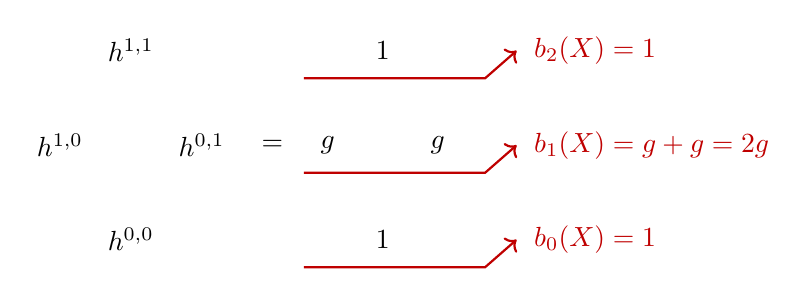
\begin{tikzpicture}[
  every node/.style={font=\normalsize},
  guide/.style={red!75!black,thick,->}
]
  % Hodge数
  \node at (0, 1.2) {$h^{1,1}$};
  \node at (-0.9,0) {$h^{1,0}$};
  \node at ( 0.9,0) {$h^{0,1}$};
  \node at (0,-1.2) {$h^{0,0}$};

  \node at (1.8,0) {$=$};

  % Hodgeダイアモンドの値
  \node at (3.2, 1.2) {$1$};
  \node at (2.5, 0)   {$g$};
  \node at (3.9, 0)   {$g$};
  \node at (3.2,-1.2) {$1$};

  % 各段の和を示す赤線
  \draw[guide]
    (2.2,0.85)--(4.5,0.85)--(4.9,1.2);
  \draw[guide]
    (2.2,-0.35)--(4.5,-0.35)--(4.9,0);
  \draw[guide]
    (2.2,-1.55)--(4.5,-1.55)--(4.9,-1.2);

  % Betti数
  \node[anchor=west,red!75!black] at (5,1.2)
    {$b_2(X)=1$};
  \node[anchor=west,red!75!black] at (5,0)
    {$b_1(X)=g+g=2g$};
  \node[anchor=west,red!75!black] at (5,-1.2)
    {$b_0(X)=1$};
\end{tikzpicture}
\end{center}

すなわち, 
\[
b_k(X)=\sum_{p+q=k}h^{p,q}(X)
\qquad(k=0,1,2)
\]
である.
特に, 中央の段の等式
\[
b_1(X)=h^{1,0}(X)+h^{0,1}(X)=2g
\]
は, Hodge分解によって
一次de Rhamコホモロジーが
次元 $g$ の二つの空間に分かれることに対応する.\footnote{
 $h^{1,1}=1$ は, 
Serreの双対定理 \ref{O-M292} による
\(
H^1(X,\Omega_X^1)
\simeq H^0(X,\mathcal O_X)^*
\simeq\mathbb C
\)
から従う.}


層コホモロジーと位相的なコホモロジーの関係は,
\[
H^1(X,\C)\simeq H_{\mathrm{DR}}^1(X,\C)
\simeq H^0(X,\Omega_X^1)\oplus H^1(X,\mathcal O_X)
\]
と表される. 左辺は特異コホモロジー, 右辺は正則な層のコホモロジーである.
高次元でも, コンパクト K\"ahler 多様体では
\[
H^k(X,\C)\simeq\bigoplus_{p+q=k}H^q(X,\Omega_X^p),
\qquad b_k(X)=\sum_{p+q=k}h^{p,q}(X)
\]
が成り立つ.







% SOURCE O:11095 | O-S060 7.4 因子に付随する有理型写像とコンパクトRiemann 面の射影埋め込み
%\subsection{因子に付随する有理型写像とコンパクトRiemann 面の射影埋め込み}\label{O-S060}

% SOURCE O:11097 | O-S061 7.4.1 因子に付随する有理型写像
\subsection{因子から定まる有理型写像}\label{O-S061}
% SOURCE O:11267 | O-S062 7.4.2 コンパクトRiemann 面の射影埋め込み定理

\begin{dfn}[完備一次系]\label{dfn-complete-linear-system}
$D$ と線形同値な効果的因子全体の集合
\[
|D|:=\{D'\mid D'\geq0,\ D'\sim D\}
\]
を $D$ の定める完備一次系という.
\end{dfn}

\begin{lem}[完備一次系と切断]\label{lem-complete-linear-system}
$X$ をコンパクトRiemann 面, $D$ を $X$ 上の因子とする.
零でない切断 $f,g\in H^0(X,\mathcal O_X(D))$ に対して,
\[
f\sim g
\quad\Longleftrightarrow\quad
g=cf\text{ となる }c\in\C^\times\text{ が存在する}
\]
と定め, $f$ の同値類を
$[f]=\{cf\mid c\in\C^\times\}$ と書く.
この同値関係による商集合を
\[
\bigl(H^0(X,\mathcal O_X(D))\setminus\{0\}\bigr)/\C^\times
\]
とする. 

このとき, 対応
\[
\bigl(H^0(X,\mathcal O_X(D))\setminus\{0\}\bigr)/\C^\times
\longrightarrow |D|,
\qquad [f]\longmapsto D+\operatorname{div}(f)
\]
は全単射である.
ここで $|D|$ は, $D$ と線形同値な効果的因子全体の集合である.

\end{lem}

特に$h^0(\mathcal O_X(D))\geq1$ ならば,
$|D|$ は次元 $h^0(\mathcal O_X(D))-1$ の射影空間とみなせる.
$h^0(\mathcal O_X(D))=0$ ならば $|D|=\emptyset$ である.

\begin{proof}
まず, 対応が矛盾なく定まることを示す.
$0\neq f\in H^0(X,\mathcal O_X(D))$ ならば,
定義\ref{O-M199}より $D+\operatorname{div}(f)\geq0$ であり,
この因子は $D$ と線形同値なので $|D|$ に属する.
また, $c\in\C^\times$ に対して,
\[
D+\operatorname{div}(cf)
=D+\underbrace{\operatorname{div}(c)}_{=0}
+\operatorname{div}(f)
=D+\operatorname{div}(f)
\]
だから, 像は代表元の選び方によらない.

全射性を示す.
$E\in|D|$ ならば, 線形同値の定義により,
零でない有理型関数 $f$ を用いて $E=D+\operatorname{div}(f)$ と書ける.
$E\geq0$ なので $f\in H^0(X,\mathcal O_X(D))$ であり,
$[f]$ の像が $E$ となる.

単射性を示す.
$[f],[g]$ の像が等しいならば,
\[
D+\operatorname{div}(f)=D+\operatorname{div}(g)
\quad\Longrightarrow\quad
\operatorname{div}(f/g)=0.
\]
従って, $f/g$ は零点も極ももたない大域的正則関数であり,
系\ref{O-M067}より零でない定数である.
よって $f,g$ は零でない定数倍だけ異なり, $[f]=[g]$ となる.
\end{proof}



\begin{dfn}[完備一次系に付随する写像]\label{O-M327}
$X$ をコンパクトRiemann 面, $D$ を $X$ 上の因子とし,
$H^0(X,\mathcal O_X(D))\neq0$ と仮定する.
その基底を
\[
\varphi_0,\ldots,\varphi_N,
\qquad N+1=\dim_{\C}H^0(X,\mathcal O_X(D))
\]
とする.

この基底から定まる写像
\[
\Phi_{|D|}:X\longrightarrow\C\mathbb P^N
\]
を, 完備一次系 $|D|$ に付随する写像という.
各成分が有限で同時には零にならない点では,
\[
\Phi_{|D|}(q)=[\varphi_0(q):\cdots:\varphi_N(q)]
\]
と定める.
\end{dfn}

\begin{rem}[局所表示と選び方への依存性]\label{O-M328}
$p\in X$ において, 基底のうち位数が最も小さいものを選び,
添字を入れ替えて $\varphi_0$ とする.
このとき,
\[
\operatorname{ord}_p\left(\frac{\varphi_i}{\varphi_0}\right)
=\operatorname{ord}_p(\varphi_i)-\operatorname{ord}_p(\varphi_0)\geq0
\]
なので, 各比は $p$ の近くで正則である.
従って, 終域の非同次座標では,
\begin{equation}\label{O-EQ096}
q\longmapsto
\left(
\frac{\varphi_1}{\varphi_0}(q),\ldots,
\frac{\varphi_N}{\varphi_0}(q)
\right)
\end{equation}
と表示できる.
つまり, 極や共通の零点があっても,
比を取ることで正則写像として延長できる.
異なる選び方による表示も, もとの写像が定義される点で一致し,
残りの点でも連続性により一致する.

また, 基底の変更は可逆行列による変換なので,
得られる写像は終域の射影変換だけ変わる.
特に, 埋め込みであるかどうかは基底によらない.

さらに, $D=D'+\operatorname{div}(\rho)$ ならば,
$\varphi\mapsto\rho\varphi$ は
$H^0(X,\mathcal O_X(D))\simeq H^0(X,\mathcal O_X(D'))$
を与える.
対応する基底では
\[
\frac{\rho\varphi_i}{\rho\varphi_0}
=\frac{\varphi_i}{\varphi_0}
\]
なので, 得られる写像は一致する.
\end{rem}

\begin{dfn}[基点と基点自由性]\label{O-M329}\label{O-M331}
$H^0(X,\mathcal O_X(D))\neq0$ とする.
すべての $E\in|D|$ に含まれる点 $q\in X$ を,
$|D|$ の基点, または底点という.
基点全体の集合を
\[
\operatorname{Bs}|D|
:=\bigcap_{E\in|D|}\operatorname{Supp}E
\]
と書く.

切断との対応（補題\ref{lem-complete-linear-system}参照）を用いると,
$q$ が基点であることは,
すべての零でない $\varphi\in H^0(X,\mathcal O_X(D))$ に対して
\[
n_q+\operatorname{ord}_q(\varphi)\geq1
\]
となることと同値である.
ここで $n_q$ は $D$ の $q$ での係数である.

$\operatorname{Bs}|D|=\emptyset$ のとき,
$|D|$ は基点自由（base point free）, または単に自由であるという.
\end{dfn}

局所座標 $t_q$ を用いると,
$t_q^{n_q}\varphi_i$ は正則に延長できる
（補題\ref{O-M205}参照）.
従って, 基底 $\varphi_0,\ldots,\varphi_N$ に対して,
\[
q\in\operatorname{Bs}|D|
\quad\Longleftrightarrow\quad
(t_q^{n_q}\varphi_i)(q)=0
\quad\text{がすべての }i\text{ で成り立つ}.
\]
ここで括弧内の値は, 正則に延長した関数の値を意味する.


\begin{rem}[基点と写像の正則性]\label{O-M330}
$p$ の局所座標を $t_p$, $D$ の $p$ での係数を $n_p$ とし,
正則関数 $f_i^p:=t_p^{n_p}\varphi_i$ を考える.

\medskip
\noindent
\textbf{(1) $p$ が基点でない場合.}
少なくとも一つの $f_j^p$ は $p$ で非零である.
従って, $p$ の近くでは各比 $f_i^p/f_j^p$ が正則となり,
これらを非同次座標として写像を定められる.
例えば $f_0^p(p)\neq0$ ならば,
\[
q\longmapsto
\left(\frac{f_1^p(q)}{f_0^p(q)},\ldots,
\frac{f_N^p(q)}{f_0^p(q)}\right)
\]
である.

\medskip
\noindent
\textbf{(2) $p$ が基点である場合.}
すべての $f_i^p(p)$ が零なので,
そのまま代入しても射影空間の点を定められない.
しかし,
\[
k:=\min_i\operatorname{ord}_p(f_i^p)\geq1,\qquad
f_i^p=t_p^k a_i
\]
と書けば, $a_i$ は正則で,
少なくとも一つの $a_i(p)$ は非零である.
$p$ を除いた近傍では
\[
[f_0^p:\cdots:f_N^p]=[a_0:\cdots:a_N]
\]
なので, 右辺を使えば $p$ にも正則に延長できる.

従って, Riemann 面では基点があっても写像は正則に延長できる.
基点自由性は, この共通因子 $t_p^k$ を取り除く操作が
どの点でも不要であることを意味する.

\medskip
\noindent
\textbf{(3) 高次元では延長できないことがある.}
例えば,
\[
\C^2\dashrightarrow\C\mathbb P^1,\qquad
(z,w)\longmapsto[z:w]
\]
では, 原点を除く $w=0$ 上で像は $[1:0]$,
$z=0$ 上で像は $[0:1]$ となる.
原点への近づき方によって極限が異なるため,
原点には連続にさえ延長できない.
\end{rem}


\begin{lem}[切断の次元による基点の判定]\label{O-M332}
$H^0(X,\mathcal O_X(D))\neq0$ とする.
任意の点 $q\in X$ に対して, 次のいずれか一方が成り立つ：
\begin{equation}\label{O-EQ097}
\dim_{\C}H^0(X,\mathcal O_X(D-q))
=\dim_{\C}H^0(X,\mathcal O_X(D)),
\end{equation}
\begin{equation}\label{O-EQ098}
\dim_{\C}H^0(X,\mathcal O_X(D-q))
=\dim_{\C}H^0(X,\mathcal O_X(D))-1.
\end{equation}
さらに, 次が成り立つ.

\smallskip
\noindent
(1) $q$ が $|D|$ の基点であることと,
\eqref{O-EQ097}が成り立つことは同値である.

\smallskip
\noindent
(2) $q$ が $|D|$ の基点でないことと,
\eqref{O-EQ098}が成り立つことは同値である.

\smallskip
従って, $|D|$ が基点自由であることは,
すべての $q\in X$ で \eqref{O-EQ098} が成り立つことと同値である.
\end{lem}

\begin{proof}
$D$ の $q$ での係数を $n_q$ とし,
$q$ を中心とする局所座標 $t_q$ を取る.
補題\ref{O-M210}の短完全系列
\[
0\longrightarrow\mathcal O_X(D-q)
\longrightarrow\mathcal O_X(D)
\longrightarrow\C_q
\longrightarrow0
\]
から, 補題\ref{O-M213}により完全系列
\begin{equation}\label{O-EQ099}
0\longrightarrow H^0(X,\mathcal O_X(D-q))
\longrightarrow H^0(X,\mathcal O_X(D))
\xrightarrow{r_q}\C
\end{equation}
を得る.
ここで,
\[
r_q:H^0(X,\mathcal O_X(D))\longrightarrow\C,
\qquad
\varphi\longmapsto(t_q^{n_q}\varphi)(q)
\]
であり, 右辺は正則に延長した関数の値を表す
（補題\ref{O-M205}参照）.

$r_q$ の終域は一次元なので, 像の次元は $0$ または $1$ である.
従って,
\[
\dim_{\C}H^0(X,\mathcal O_X(D))
\underalign{\text{(次元公式)}}{=}
\underbrace{\dim_{\C}\ker r_q}_{
=\dim_{\C}H^0(X,\mathcal O_X(D-q))\ \text{(完全性)}}
+\underbrace{\dim_{\C}\operatorname{Im}r_q}_{=0\text{ または }1}.
\]
よって, \eqref{O-EQ097}, \eqref{O-EQ098}のいずれか一方が成り立つ.

次に, 定義\ref{O-M329}の基点条件から,
\begin{equation}\label{O-EQ100}
q\in\operatorname{Bs}|D|
\quad\Longleftrightarrow\quad
r_q(\varphi)=0\text{ がすべての切断 }\varphi\text{ で成り立つ}
\quad\Longleftrightarrow\quad
\operatorname{Im}r_q=\{0\}.
\end{equation}
従って, 上の次元公式より,
$q$ が基点であることと \eqref{O-EQ097} が成り立つことは同値である.

一方, $q$ が基点でなければ,
$r_q(\varphi)\neq0$ となる切断が存在する.
終域が一次元なので,
\begin{equation}\label{O-EQ101}
q\notin\operatorname{Bs}|D|
\quad\Longleftrightarrow\quad
\operatorname{Im}r_q=\C.
\end{equation}
従って, $q$ が基点でないことと \eqref{O-EQ098} が成り立つことは同値である.
\end{proof}



\subsection{コンパクトRiemann 面は射影多様体であり代数多様体である}
\label{O-S062}

本節では, 次数が十分大きい因子から, 
コンパクトRiemann 面の射影埋め込みを構成する.

\begin{thm}[コンパクトRiemann 面の射影埋め込み定理]
\label{O-M333}
$X$ を種数 $g$ のコンパクトRiemann 面, 
$D$ を $X$ 上の因子とする.

\medskip
\noindent
\textbf{(1)}
$\deg D\geq2g$ ならば, $|D|$ は基点自由である.
従って, 付随する写像
\[
\Phi_{|D|}:X\longrightarrow\C\mathbb P^N,
\qquad
N=\dim_{\mathbb C}H^0(X,\mathcal O_X(D))-1
\]
は正則写像である.

\medskip
\noindent
\textbf{(2)}
$\deg D\geq2g+1$ ならば, $\Phi_{|D|}$ は正則埋め込みである.

特に, 任意の点 $p\in X$ に対して, 
因子 $(2g+1)p$ は正則埋め込み
\[
\Phi_{|(2g+1)p|}:X\hookrightarrow\C\mathbb P^{g+1}
\]
を与える.
従って, 任意のコンパクトRiemann 面は, 
射影空間の閉複素部分多様体として実現できる.
\end{thm}

証明の準備として, 切断の値と一次微分を指定できることを示す.


\begin{lem}[切断の値と一次微分の指定]
\label{O-M334}\label{O-M335}\label{O-M336}
$X$ を種数 $g$ のコンパクトRiemann 面, $D$ を因子とする.
各点 $p$ で, $D$ の係数を $n_p$,
$p$ を中心とする局所座標を $t_p$ とし,
$f_p:=t_p^{n_p}$ とおく.
このとき, 次が成り立つ.

\medskip
\noindent
(1) $\deg D\geq2g$ ならば, 任意の点 $p$ に対して,
\[
r_p:H^0(X,\mathcal O_X(D))\longrightarrow\C,
\qquad \varphi\longmapsto(f_p\varphi)(p)
\]
は全射である.

\medskip
\noindent
(2) $\deg D\geq2g+1$ ならば, 任意の異なる二点 $p,q$ に対して,
\[
r_p\oplus r_q:H^0(X,\mathcal O_X(D))\longrightarrow\C^2,
\qquad
\varphi\longmapsto\bigl((f_p\varphi)(p),(f_q\varphi)(q)\bigr)
\]
は全射である.

\medskip
\noindent
(3) $\deg D\geq2g+1$ ならば, 任意の点 $p$ に対して,
\[
r_{2p}:H^0(X,\mathcal O_X(D))
\longrightarrow\C\{t_p\}/(t_p^2),
\qquad
\varphi\longmapsto f_p\varphi\bmod(t_p^2)
\]
は全射である.
\end{lem}
\begin{proof}
(1) 補題\ref{O-M210}より, 短完全系列
\begin{equation}\label{O-EQ102}
0\longrightarrow\mathcal O_X(D-p)
\longrightarrow\mathcal O_X(D)
\longrightarrow\C_p
\longrightarrow0
\end{equation}
がある.
右の写像は, $p$ の近くで
$\varphi\mapsto(t_p^{n_p}\varphi)(p)$ と表される.

仮定より,
\[
\deg(D-p)=\deg D-1
\underalign{\text{(仮定 $\deg D\geq2g$)}}{\geq}2g-1
\]
なので, 系\ref{O-M301}から
$H^1(X,\mathcal O_X(D-p))=0$ である.
従って, 定理\ref{O-M234}の長完全系列から,
\begin{equation}\label{O-EQ103}
H^0(X,\mathcal O_X(D))
\xrightarrow{r_p}\C
\longrightarrow
\underbrace{H^1(X,\mathcal O_X(D-p))}_{=0}
\end{equation}
は完全である.
よって,
\[
\operatorname{Im}r_p
\underalign{\text{(完全性)}}{=}
\ker(\C\longrightarrow0)=\C
\]
となり, $r_p$ は全射である.

\medskip
\noindent
(2) 補題\ref{O-M210}より, 短完全系列
\begin{equation}\label{O-EQ104}
0\longrightarrow\mathcal O_X(D-p-q)
\longrightarrow\mathcal O_X(D)
\longrightarrow\C_p\oplus\C_q
\longrightarrow0
\end{equation}
がある.
右の写像は, $p,q$ でそれぞれ
$(t_p^{n_p}\varphi)(p)$, $(t_q^{n_q}\varphi)(q)$ を取る写像である.

仮定より,
\[
\deg(D-p-q)=\deg D-2
\underalign{\text{(仮定 $\deg D\geq2g+1$)}}{\geq}2g-1.
\]
従って, 系\ref{O-M301}と定理\ref{O-M234}により,
\begin{equation}\label{O-EQ105}
H^0(X,\mathcal O_X(D))
\xrightarrow{r_p\oplus r_q}\C^2
\longrightarrow
\underbrace{H^1(X,\mathcal O_X(D-p-q))}_{=0}
\end{equation}
は完全である.
(1) と同様に, $r_p\oplus r_q$ は全射となる.

\medskip
\noindent
(3) $p$ に集中し, ストークが $\C\{t_p\}/(t_p^2)$ である
摩天楼層を $\mathcal S_{2p}$ とする.
補題\ref{O-M210}より, 短完全系列
\begin{equation}\label{O-EQ106}
0\longrightarrow\mathcal O_X(D-2p)
\longrightarrow\mathcal O_X(D)
\longrightarrow\mathcal S_{2p}
\longrightarrow0
\end{equation}
がある.
右の写像は, $p$ の近くで
$\varphi\mapsto t_p^{n_p}\varphi\bmod(t_p^2)$ と表される.
ここで,
\[
t_p^{n_p}\varphi
\equiv
\underbrace{(t_p^{n_p}\varphi)(p)}_{\text{値}}
+\underbrace{\frac{d(t_p^{n_p}\varphi)}{dt_p}(p)}_{\text{一次微分}}t_p
\pmod{t_p^2}
\]
なので, この写像は値と一次微分を取り出す写像である.

また,
\[
\deg(D-2p)=\deg D-2
\underalign{\text{(仮定 $\deg D\geq2g+1$)}}{\geq}2g-1.
\]
従って, 系\ref{O-M301}と定理\ref{O-M234}により,
\begin{equation}\label{O-EQ107}
H^0(X,\mathcal O_X(D))
\xrightarrow{r_{2p}}\C\{t_p\}/(t_p^2)
\longrightarrow
\underbrace{H^1(X,\mathcal O_X(D-2p))}_{=0}
\end{equation}
は完全であり, $r_{2p}$ も全射である.
\end{proof}


\begin{proof}[定理\ref{O-M333}の証明]
補題\ref{O-M334}の三つの全射性を用いて,
基点自由性, 写像の単射性, 微分の単射性を順に示す.
各点 $p$ で, $D$ の係数を $n_p$,
$p$ を中心とする局所座標を $t_p$ とする.

\medskip
\noindent
\textbf{(1) 基点自由性.}

$\deg D\geq2g$ とする.
補題\ref{O-M334}(1)により, 任意の点 $p$ に対して,
\[
(t_p^{n_p}\varphi)(p)=1
\]
となる大域切断 $\varphi$ が存在する.
従って $p$ は基点ではない（定義\ref{O-M329}参照）.
$p$ は任意なので $|D|$ は基点自由であり,
$\Phi_{|D|}$ は正則写像となる（補足\ref{O-M330}参照）.

以下では $\deg D\geq2g+1$ と仮定する.
基底の変更は終域の射影変換に対応するので,
単射性や微分の単射性を調べる際には,
都合のよい基底を選んでよい（補足\ref{O-M328}参照）.

\medskip
\noindent
\textbf{(2) 異なる二点を区別すること.}

$p\neq q$ を取る.
補題\ref{O-M334}(2)により, 大域切断 $\psi_0,\psi_1$ を
\[
\begin{array}{c|cc}
 & p\text{ での値} & q\text{ での値}\\ \hline
\psi_0 & (t_p^{n_p}\psi_0)(p)=1 & (t_q^{n_q}\psi_0)(q)=0\\
\psi_1 & (t_p^{n_p}\psi_1)(p)=0 & (t_q^{n_q}\psi_1)(q)=1
\end{array}
\]
となるように選べる.
これらは一次独立なので, 基底
$\psi_0,\psi_1,\ldots,\psi_N$ に延長できる.

この基底による局所表示から,
\[
\Phi_{|D|}(p)=[1:0:\cdots],\qquad
\Phi_{|D|}(q)=[0:1:\cdots]
\]
となる.
第一成分が一方では非零, 他方では零なので, 両者は異なる.
従って, $\Phi_{|D|}$ は単射である.

\medskip
\noindent
\textbf{(3) 各点で微分が単射であること.}

$p\in X$ を固定する.
補題\ref{O-M334}(3)により, 大域切断 $\psi_0,\psi_1$ を
\[
t_p^{n_p}\psi_0\equiv1\pmod{t_p^2},
\qquad
t_p^{n_p}\psi_1\equiv t_p\pmod{t_p^2}
\]
となるように選べる.
その像 $1,t_p$ は一次独立なので,
$\psi_0,\psi_1$ も一次独立であり, 基底に延長できる.

$(t_p^{n_p}\psi_0)(p)=1$ なので,
$p$ の近くでの非同次座標表示は
\[
q\longmapsto
\left(
\frac{t_p^{n_p}\psi_1}{t_p^{n_p}\psi_0}(q),\ldots,
\frac{t_p^{n_p}\psi_N}{t_p^{n_p}\psi_0}(q)
\right)
\]
である.
その第一成分は,
\[
\frac{t_p^{n_p}\psi_1}{t_p^{n_p}\psi_0}
=\frac{t_p+O(t_p^2)}{1+O(t_p^2)}
=t_p+O(t_p^2)
\]
となる.
従って,
\[
\frac{d}{dt_p}
\left(\frac{t_p^{n_p}\psi_1}{t_p^{n_p}\psi_0}\right)(p)
=1\neq0.
\]
少なくとも一つの座標成分の微分が非零なので,
$d\Phi_{|D|}(p)$ は零写像ではない.
始域の接空間は一次元だから,
\[
d\Phi_{|D|}(p):
\underbrace{T_pX}_{\dim_{\C}=1}
\longrightarrow T_{\Phi_{|D|}(p)}\C\mathbb P^N
\]
は単射である.

以上より, $\Phi_{|D|}$ は単射で, 各点で微分も単射である.
$X$ はコンパクトなので,
定義\ref{O-M128}により $\Phi_{|D|}$ は正則埋め込みとなる.
また, その像はコンパクトなので閉集合である.

最後に $D=(2g+1)p$ と取ると,
\[
\dim_{\C}H^0(X,\mathcal O_X((2g+1)p))
\underalign{\text{(系\ref{O-M302})}}{=}
\underbrace{\deg((2g+1)p)}_{=2g+1}+1-g
=g+2.
\]
従って, この $g+2$ 個の基底切断から,
$\C\mathbb P^{g+1}$ への正則埋め込みが得られる.
\end{proof}


\begin{rem}[消滅定理が埋め込みを与える仕組み]
証明で用いた対応は, 次の表にまとめられる.
\[
\begin{array}{c|c|c}
\text{消滅する群}
& \text{指定できるデータ}
& \text{幾何学的な帰結}\\ \hline
H^1(X,\mathcal O_X(D-p))
& p\text{ での値}
& \text{基点がない}\\[4pt]
H^1(X,\mathcal O_X(D-p-q))
& p,q\text{ での値}
& \text{異なる二点を区別する}\\[4pt]
H^1(X,\mathcal O_X(D-2p))
& p\text{ での値と一次微分}
& \text{微分が単射になる}
\end{array}
\]
ここで二段目では $p\neq q$ とする.
消滅定理によって局所的なデータを大域切断で実現し, 
それを射影座標として使うことが, 証明の中心である.
\end{rem}

コンパクトRiemann 面は代数多様体であることを示そう. 
これには大結果を用いることになる. 

\begin{dfn}[射影多様体と射影埋め込み]\label{O-M340}
複素多様体 $Y$ が, ある射影空間 $\C\mathbb P^N$ の
閉複素部分多様体と双正則であるとき, 
$Y$ を射影多様体という.
ここでは, 非特異な射影多様体のみを考える.

また, 正則写像
\[
f:Y\longrightarrow\C\mathbb P^N
\]
が, その像 $f(Y)$ を閉複素部分多様体とし, 
\[
f:Y\xrightarrow{\sim}f(Y)
\]
が双正則写像であるとき, $f$ を射影埋め込みという.
\end{dfn}


\begin{thm}[Chowの定理]\label{O-M341}
$Y\subset\C\mathbb P^N$ を閉複素部分多様体とする.
このとき, 有限個の同次多項式
\[
F_1,\ldots,F_m\in\mathbb C[X_0,\ldots,X_N]
\]
が存在して, 
\begin{equation}\label{O-EQ108}
Y=
\left\{
[X_0:\cdots:X_N]\in\C\mathbb P^N
\ \middle|\
F_1(X_0,\ldots,X_N)=\cdots=F_m(X_0,\ldots,X_N)=0
\right\}
\end{equation}
となる.
\end{thm}

Chowの定理の証明は省略する.
射影埋め込み定理と組み合わせると, 次の結論を得る.

\begin{cor}[コンパクトRiemann 面の代数性]\label{O-M342}
任意のコンパクトRiemann 面 $X$ は, 
非特異射影代数曲線と双正則である.

すなわち, ある射影空間 $\C\mathbb P^N$ 内の, 
有限個の同次多項式の共通零点集合である非特異な曲線 $Y$ と, 
双正則写像
\(
X\xrightarrow{\sim}Y
\)
が存在する.
\end{cor}

\begin{proof}
定理 \ref{O-M333} により, 射影埋め込み
\[
f:X\hookrightarrow\C\mathbb P^N
\]
が存在する.
その像 $f(X)$ は一次元の閉複素部分多様体である.
Chowの定理 \ref{O-M341} より, 
$f(X)$ は非特異射影代数曲線であり, 
$f$ は $X$ とこの曲線との双正則同型を与える.
\end{proof}

以上より, 射影埋め込み定理とChowの定理によって, 
次の二つの見方が結び付く.

\begin{center}
\renewcommand{\arraystretch}{1.4}
\begin{tabular}{c|c|c}
 & 複素解析の立場 & 代数幾何学の立場 \\ \hline
対象
& コンパクトRiemann 面
& 非特異射影代数曲線 \\
記述の方法
& 局所座標と正則な座標変換
& 有限個の同次多項式の方程式
\end{tabular}
\end{center}

複素代数幾何学の研究手法がいろいろある(代数・幾何・解析)のはこのためである. 
どの方法を用いても良い. 

\subsection{豊富因子}
定理 \ref{O-M333} の証明では, 
大域切断によって二点の値や一点での一次微分を指定することで, 
射影埋め込みを構成した.
この議論から, 切断の次元を用いた次の判定法が得られる.

\begin{prop}[埋め込み判定法]\label{O-M346}

$X$ をコンパクトRiemann 面, $D$ を $X$ 上の因子とする.
任意の二点 $p,q\in X$（$p=q$ の場合も含む）について
\[
\dim_{\mathbb C}H^0(X,\mathcal O_X(D-p-q))
=
\dim_{\mathbb C}H^0(X,\mathcal O_X(D))-2
\]
が成り立つならば, 次の二つが成り立つ.
\begin{enumerate}
\item $|D|$ は基点自由である.
\item 付随する写像
\[
\Phi_{|D|}:X\longrightarrow\C\mathbb P^N,
\qquad
N=\dim_{\mathbb C}H^0(X,\mathcal O_X(D))-1
\]
は正則埋め込みである.
\end{enumerate}
\end{prop}
\begin{proof}
$p\neq q$ のときは二点での値を取る写像 $r_p\oplus r_q$,
$p=q$ のときは値と一次微分を取る写像 $r_{2p}$ を考える.
これらは補題\ref{O-M334}で用いた写像であり,
次数の仮定によらず定義される.

いずれも終域は二次元で, 核は
$H^0(X,\mathcal O_X(D-p-q))$ である.
従って,
\[
\dim_{\C}\operatorname{Im}r
\underalign{\text{(次元公式)}}{=}
\dim_{\C}H^0(X,\mathcal O_X(D))
-\underbrace{\dim_{\C}H^0(X,\mathcal O_X(D-p-q))}_{
=\dim_{\C}H^0(X,\mathcal O_X(D))-2\ \text{(仮定)}}
=2
\]
となり, どちらの写像も全射である.

よって, 二点での値と一点での値・一次微分を任意に指定できる.
定理\ref{O-M333}の証明と同様に,
$|D|$ は基点自由であり,
$\Phi_{|D|}$ は単射かつ各点で微分が単射となる.
$X$ のコンパクト性と定義\ref{O-M128}から,
$\Phi_{|D|}$ は正則埋め込みである.
\end{proof}

\begin{dfn}[非常に豊富な因子と豊富な因子]\label{O-M348}
$X$ 上の因子 $D$ に対して, 次のように定める.
\begin{itemize}
\item
$|D|$ が基点自由であり, 
$\Phi_{|D|}$ が正則埋め込みを与えるとき, 
$D$ を非常に豊富な因子（very ample divisor）という.

\item
ある正の整数 $n$ に対して $nD$ が非常に豊富であるとき, 
$D$ を豊富な因子（ample divisor）という.
\end{itemize}
つまり, 非常に豊富な因子はそのままで射影埋め込みを与え, 
豊富な因子は適切な正の整数倍を取ることで射影埋め込みを与える.
\end{dfn}

\begin{cor}[豊富性の次数による判定]\label{O-M349}
コンパクトRiemann 面 $X$ 上の因子 $D$ に対して, 
\[
D\text{ が豊富}
\quad\Longleftrightarrow\quad
\deg D>0
\]
が成り立つ.
\end{cor}
\begin{proof}
$\deg D>0$ ならば, 十分大きい整数 $n$ に対して
$\deg(nD)=n\deg D\geq2g+1$ となる.
定理\ref{O-M333}より $nD$ は非常に豊富なので,
定義\ref{O-M348}より $D$ は豊富である.

逆に, $D$ が豊富ならば, ある $n\geq1$ に対して $nD$ は非常に豊富であり,
$h^0(\mathcal O_X(nD))\geq2$ である.
零でない切断 $\varphi$ を取り,
$E:=nD+\operatorname{div}(\varphi)\geq0$ とおくと,
\[
0\leq\deg E
=n\deg D+\underbrace{\deg\operatorname{div}(\varphi)}_
{=0\ \text{(補題\ref{O-M198})}}
=n\deg D.
\]
もし $\deg D=0$ ならば, 効果的因子 $E$ の次数が $0$ なので $E=0$ となる.
従って $nD\sim0$ であり,
\[
h^0(\mathcal O_X(nD))
\underalign{\text{(線形同値)}}{=}
h^0(\mathcal O_X)
\underalign{\text{(系\ref{O-M067})}}{=}1
\]
となって矛盾する.
よって $\deg D>0$ である.
\end{proof}

% プリアンブルに追加：
% \usepackage{amsmath,amssymb}
% \usepackage{graphicx}
% \usepackage{tikz}
\subsection{Riemann 面の粗い分類と極小モデル理論}


系\ref{O-M298}と系\ref{O-M349}を組み合わせると次を得る. 
\begin{cor}
コンパクトRiemann 面 $X$ では, 
\[
\deg K_X=2g-2
\]
である.
従って, 系 \ref{O-M349} より, 
$K_X$ が豊富であることと $g\geq2$ は同値である.
\end{cor}

コンパクトRiemann 面 $X$ は一意化定理によって,
複素構造に適合する定曲率計量を選ぶことができる. \footnote{一意化定理は, 単連結Riemann 面が球面, 複素平面, 単位円板のいずれかと双正則であるという定理である. コンパクトRiemann 面の普遍被覆にこれを用いると, 球面・平坦・双曲計量から, それぞれ種数 $0$, $1$, $2$ 以上に対応する定曲率計量が得られる. 複素構造に適合するとは, 局所座標 $z$ で計量が $\lambda(z)|dz|^2$（$\lambda>0$）と書けることである. 表では曲率が $1,0,-1$ となるように規格化している.}

この計量のKähler形式を $\omega$ とすると, 
種数に応じて次のように整理できる.

\begin{center}
\resizebox{\linewidth}{!}{%
\begin{tikzpicture}[
  every node/.style={font=\normalsize,align=center},
  surface/.style={draw=blue!65!black,thick},
  rim/.style={draw=blue!65!black,thick}
]
  % 表の背景
  \fill[blue!3] (0,0) rectangle (2.4,7.2);
  \fill[blue!2] (2.4,4.15) rectangle (13.8,7.2);

  % 表の枠
  \draw[thick] (0,0) rectangle (13.8,7.2);
  \foreach \x in {2.4,6.2,10}{
    \draw[thick] (\x,0)--(\x,7.2);
  }
  \foreach \y in {1,2.15,3.15,4.15}{
    \draw[thick] (0,\y)--(13.8,\y);
  }

  % 左端の見出し
  \node at (1.2,5.68) {位相的な形};
  \node at (1.2,3.65) {Ricci 曲率};
  \node at (1.2,2.65) {種数};
  \node at (1.2,1.575) {標準因子};
  \node at (1.2,0.5) {名称};

  % 球面
  \begin{scope}[shift={(4.3,5.7)}]
    \shade[ball color=blue!55,surface]
      (0,0) circle (1);
  \end{scope}

  % トーラス：位相的な模式図
  \begin{scope}[shift={(8.1,5.7)}]
    \shade[ball color=blue!55,surface]
      (0,0) ellipse (1.45 and 0.85);

    \filldraw[fill=white,rim]
      (0,0.10) ellipse (0.75 and 0.31);

    \draw[blue!35,line width=2pt]
      (-1.18,-0.22)
      .. controls (-0.65,-0.90) and (0.65,-0.90) ..
      (1.18,-0.22);
  \end{scope}

  % 種数2の曲面：g>=2 の代表的な模式図
  \begin{scope}[shift={(11.9,5.7)}]
    \path[shade,ball color=blue!55,surface]
      (-1.5,0)
      .. controls (-1.5,0.80) and (-0.80,1.02) ..
      (-0.25,0.70)
      .. controls (-0.08,0.60) and (0.08,0.60) ..
      (0.25,0.70)
      .. controls (0.80,1.02) and (1.5,0.80) ..
      (1.5,0)
      .. controls (1.5,-0.80) and (0.80,-1.02) ..
      (0.25,-0.70)
      .. controls (0.08,-0.60) and (-0.08,-0.60) ..
      (-0.25,-0.70)
      .. controls (-0.80,-1.02) and (-1.5,-0.80) ..
      (-1.5,0)
      -- cycle;

    \filldraw[fill=white,rim]
      (-0.73,0.10) ellipse (0.48 and 0.29);
    \filldraw[fill=white,rim]
      (0.73,0.10) ellipse (0.48 and 0.29);

    \node[font=\small] at (0,-1.18) {図は $g=2$ の場合};
  \end{scope}

  % Ricci 曲率
  \node at (4.3,3.65)
    {$\operatorname{Ric}(\omega)=\omega>0$};
  \node at (8.1,3.65)
    {$\operatorname{Ric}(\omega)=0$};
  \node at (11.9,3.65)
    {$\operatorname{Ric}(\omega)=-\omega<0$};

  % 種数
  \node at (4.3,2.65) {$g=0$};
  \node at (8.1,2.65) {$g=1$};
  \node at (11.9,2.65) {$g\geq2$};

  % 標準因子
  \node at (4.3,1.575)
    {$-K_X$ が豊富\\[-1pt]
     $\deg K_X=-2$};
  \node at (8.1,1.575)
    {$K_X\sim0$\\[-1pt]
     $\deg K_X=0$};
  \node at (11.9,1.575)
    {$K_X$ が豊富\\[-1pt]
     $\deg K_X=2g-2>0$};

  % 名称
  \node at (4.3,0.5) {Fano};
  \node at (8.1,0.5) {Calabi--Yau};
  \node at (11.9,0.5)
    {Canonically polarized\\[-1pt]
     \small 一般型};
\end{tikzpicture}%
}
\end{center}
注意として$K_X\sim0$ は, 標準束が自明であることを意味する.
表では, この意味で種数 $1$ の曲線を
Calabi--Yau と呼んでいる.\footnote{この定義MMPの人が使うCalabi-Yauである. 強い意味のCalabi-Yauもあるので注意.ミラー対称性などで出てくるのは後者だと思う. }
また, canonically polarized とは, 
標準束が豊富であることを意味する.
コンパクトRiemann 面では, これは一般型であることと同値である.\footnote{一般型とは$K_X$が巨大(big)となること補足\ref{rem-ample-big}も参照. 豊富ならば巨大であるが一般には逆は成り立たない. ただ一次元なら逆も言える}

では高次元の時はどうなるのだろうか？
このような3つ(Fano, Calabi--Yau, 一般型)で構成されるのだろうか？
このような多様体の構造を, 双有理変換を用いて調べるのが
\textbf{極小モデル理論}
（minimal model program, 略して MMP）である.後の補足\ref{rem-mmp}も参照されたい.

大まかにいえば, 上の三つの型を基本的な部品とみなし,
双有理変換とファイブレーションを通じて,
高次元の多様体の構造を理解することを目指す理論である.\footnote{と勝手に思っているが, 岩井はMMPの専門家ではないので注意が必要である. ただICM 2018 で公開された Caucher Birkarの動画を見る限りそう思った方がわかりやすいと思う}

この考え方のわかりやすい紹介として,
ICM 2018 で公開された Caucher Birkar の
フィールズ賞受賞紹介動画（約 $5$ 分）を挙げておく.
\url{https://www.youtube.com/watch?v=KPTEkNZ4XCk}


\subsection{Kodaira 埋め込み定理・Nakai--Moishezon判定法・Fujita 予想}
% SOURCE O:11796 | O-M350 eg 7.32; original option: 例 7.32
教科書にはこの部分に関して次の記載があった.
\begin{tcolorbox}[mybox]
次の定理はコンパクトRiemann 面はすべて射影空間に埋め込めてしまうことを主張する非常に意外な定理である. 同様のことは $2$ 次元以上のコンパクト複素多様体に対しては一般に成立しない. 
またこの定理はいわゆるKodaira 埋め込み定理の原形である. ここで述べた形は近年その高次元化が活発に研究されているFujita 予想といわれている予想の最初の根拠でもある.
\end{tcolorbox}
Fujita 予想に関して記載があるのは驚きである. \footnote{Fujita 予想の"藤田"は藤田隆夫先生のこと. 阪大の藤田健人先生ではない.}教科書が刊行されたのは2002年のことなので, かなり盛んだったのかもしれない. 


% 予想環境が未定義の場合は, プリアンブルに追加：
% \newtheorem{conj}[thm]{予想}

\begin{rem}[Kodaira 埋め込み定理とNakai--Moishezon の豊富性判定法]


コンパクトRiemann 面の射影埋め込み定理は, 
高次元では次のKodaira 埋め込み定理につながる.

\begin{thm}[Kodaira 埋め込み定理]
$X$ をコンパクト複素多様体, $L$ を $X$ 上の正則直線束とする.
$L$ が曲率正の滑らかなHermite計量をもつならば, 
ある正の整数 $m_0$ が存在し, すべての $m\geq m_0$ に対して
$L^{\otimes m}$ の大域切断は射影埋め込み
\[
X\hookrightarrow
\mathbb P\bigl(H^0(X,L^{\otimes m})^*\bigr)
\]
を与える.
特に, 
\[
\text{$L$ が豊富}
\quad\Longleftrightarrow\quad
\text{$L$は曲率正の計量をもつ}.
\]
\end{thm}
$X$ をコンパクトRiemann 面, $D$ を $X$ 上の因子とし, 
$L=\mathcal O_X(D)$ を対応する正則直線束とする.
Kodaira 埋め込み定理と系 \ref{O-M349} を合わせると, 
\[
\deg D>0
\quad\Longleftrightarrow\quad
L\text{ が豊富}
\quad\Longleftrightarrow\quad
L\text{ が曲率正の滑らかなHermite計量をもつ}
\]
となる.
つまり, 一次元では, 直線束の曲率を正にできるかどうかが, 
次数という一つの整数によって判定できる.

高次元だとどうなるのだろうか？これは実はこれも高次元化できる. 
\begin{thm}[Nakai--Moishezon の豊富性判定法]
$X$ を非特異複素射影多様体, 
$D$ を $X$ 上の因子とし, $L=\mathcal O_X(D)$ とおく.

正次元の既約閉代数部分集合 $V\subset X$ に対し, 
$k=\dim V$ として, 交点数を
\[
(D^k\cdot V):=\int_V c_1(L)^k
\]
と書く.
ここで $c_1(L)$ は $L$ の第一 Chern 類であり, 
積分は $V$ の基本類とのペアリングを表す.
この交点数は, 曲線上の直線束の次数の高次元版である.

このとき, 次の二つの条件は同値である.
\begin{itemize}
\item $D$ は豊富である.
\item すべての正次元の既約閉代数部分集合 $V\subset X$ に対して, 
\[
(D^{\dim V}\cdot V)>0
\]
が成り立つ. なお$V=X$ も含め, $V$ の非特異性は仮定しない.
\end{itemize}
\end{thm}


Nakai--Moishezon の判定法とKodaira 埋め込み定理を合わせると, 
次の表の各列にある三つの条件は同値である.

\begin{center}
\renewcommand{\arraystretch}{1.6}
\begin{tabular}{c|c|c}
 & $\dim X=1$ & $\dim X=n$ \\ \hline
数値的な条件
& $\deg D>0$
& $\displaystyle
   \int_V c_1(L)^{\dim V}>0
   \quad(\text{すべての }V)$ \\[3pt]
代数幾何学的な条件
& $L$ が豊富
& $L$ が豊富 \\
複素幾何学的な条件
& 曲率正の滑らかな計量をもつ
& 曲率正の滑らかな計量をもつ
\end{tabular}
\end{center}
\end{rem}

\begin{rem}[Fujita 予想]
豊富な因子 $A$ は, 十分大きな整数倍を取れば
射影埋め込みを与える.
Fujita 予想は, 標準因子 $K_X$ を加えることで, 
必要な倍数を $X$ の次元だけから決められると主張する.

\begin{conj}[Fujita 予想]
$X$ を複素 $n$ 次元の非特異射影多様体, 
$A$ を豊富な因子とする.ただし $n\geq1$ とする.


このとき, 次が成り立つ.
\begin{enumerate}
\item $m\geq n+1$ ならば $|K_X+mA|$ は基点自由である.
\item $m\geq n+2$ ならば $K_X+mA$ は非常に豊富である.
\end{enumerate}
ここで $K_X$ は, 標準束
$\bigwedge^n\Omega_X^1$ に対応する標準因子である.
\end{conj}

この予想の特徴は, 倍数の条件が
$X$ や $A$ の個別の性質によらず, 
次元 $n$ だけで与えられることである.
曲線の場合には, すでに示した埋め込み定理から従う.

\begin{cor}[Fujita 予想の一次元の場合]
$X$ をコンパクトRiemann 面, $A$ を豊富な因子とする.
このとき, 
\[
m\geq2
\quad\Longrightarrow\quad
|K_X+mA|\text{ は基点自由},
\]
\[
m\geq3
\quad\Longrightarrow\quad
K_X+mA\text{ は非常に豊富}
\]
である.
\end{cor}

\begin{proof}
系\ref{O-M349}より $\deg A\geq1$, 系\ref{O-M298}より $\deg K_X=2g-2$ なので,
$\deg(K_X+mA)\geq2g-2+m$ である. 従って定理\ref{O-M333}の (1), (2) を適用すればよい.
\end{proof}

Fujita 予想の$|K_X+mA|$ の基点自由性について, 次の結果がある.

\begin{itemize}
\item
\textbf{Angehrn--Siu（1995年）：}
\[
m\geq\frac{n(n+1)}2+1
\]
ならば基点自由である.多変数複素解析を用いるブレイクスルーであった. 

\item
\textbf{Helmke（1997年, 1999年）：}
特異点の重複度の評価を用いた, 
基点自由性の数値的判定法を発展させた.代数幾何学的な証明である. 

\item
\textbf{Heier（2001年のプレプリント）：}
Angehrn--Siu と Helmke の方法を組み合わせ, 
基点自由性を保証する倍数の評価を
$O(n^{4/3})$ に改良した.

\item
\textbf{Ghidelli--Lacini（2024年）：}
$n\geq2$ のとき, 
\[
m\geq n\bigl(\log\log n+2.34\bigr)
\]
ならば基点自由である.ここで $\log$ は自然対数である.Helmkeの手法を洗練したものである. 

\item
\textbf{Jingjun Han（2026年9月のプレプリント）：}
\[
m\geq\lceil C_0n\rceil,\qquad C_0=1.77629\ldots
\]
ならば基点自由であるという一次の評価を主張している.
\end{itemize}

\end{rem}


\newpage
\section{コンパクトRiemann 面の分類}
% SOURCE O:11803 | O-S063 7.5 種数 $0,1$ のコンパクトRiemann 面の構造
コンパクトRiemann 面を種数$g$によって分類していこう. 今回は種数$4$までの分類を目指す. 
以下, 断りがなければ$X$ を種数$g$のコンパクトRiemann 面とする.

\subsection{関数体}
この部分は難しい.体論の言葉が多いからである. 証明を一応書いておくが, 飛ばして良い. 
今後使う内容は下の定理と, 超楕円曲線の関数体 \ref{O-M280}ぐらいである. 
\begin{thm}[{=定理 \ref{thm-function-field-determines-surface}}]
$X,Y$ をコンパクトRiemann 面とする.
このとき, 
\[
X\simeq Y
\quad\Longleftrightarrow\quad
\mathcal M(X)\simeq_{\mathbb C}\mathcal M(Y)
\]
である.
左辺は双正則同型, 右辺は定数関数を固定する体の同型を表す.
\end{thm}
上において$X$ 上の大域的有理型関数全体は体をなし,
これを有理型関数体 $\mathcal M(X)$ という
（定義\ref{O-M056}参照）.
例えば, $\mathcal M(\C\mathbb P^1)=\C(z)$ である
（命題\ref{O-M022}参照）.



\begin{thm}[有理型関数体の構造]\label{O-M274}
$X$ をコンパクトRiemann 面とし,
$f\in\mathcal M(X)$ を定数でない有理型関数とする.
対応する正則写像
$\widetilde f:X\to\C\mathbb P^1$ の次数を $d$ とする.

このとき, ある $h\in\mathcal M(X)$ が存在し,
任意の $k\in\mathcal M(X)$ は一意に
\[
k=A_0(f)+A_1(f)h+\cdots+A_{d-1}(f)h^{d-1},
\qquad A_j(T)\in\C(T)
\]
と書ける.
すなわち, $1,h,\ldots,h^{d-1}$ は
$\C(f)$ 上の線形空間 $\mathcal M(X)$ の基底であり,
\[
\mathcal M(X)=\C(f,h),\qquad
[\mathcal M(X):\C(f)]=d
\]
である.
\end{thm}
つまり一般の $X$ でも, 二つの有理型関数を用いれば,
すべての有理型関数を表せる.
そして一般のファイバー $\widetilde f^{-1}(q)$ の点の個数 $d$ が,
$\mathcal M(X)$ を $\C(f)$ 上の線形空間として表すときの
基底の個数に一致する, という定理である.

\begin{rem}[体論の用語]
上の定理で用いる用語と, その帰結をまとめる.
\begin{itemize}
\item \textbf{元が生成する体.}
$\C(f)$ は, $f$ の有理式全体からなる体である：
\[
\C(f)=\left\{
\frac{P(f)}{Q(f)}
\ \middle|\
P,Q\in\C[T],\ Q(f)\neq0
\right\}.
\]
同様に, $\C(f,h)$ は $f,h$ の有理式全体からなる体である.
従って $\mathcal M(X)=\C(f,h)$ とは,
すべての大域的有理型関数が $f,h$ の有理式で書けることを意味する.

\item \textbf{体の拡大と拡大次数.}
体の包含 $K\subset L$ を体の拡大という.
$L$ は $K$ 上の線形空間とみなせるので, その次元を
\[
[L:K]:=\dim_K L
\]
と書き, 拡大次数という.
この次元が有限ならば, $L/K$ は有限次拡大であるという.
定理\ref{O-M274}では,
$K=\C(f)$, $L=\mathcal M(X)$ とすると拡大次数が $d$ になる.

\item \textbf{代数的な元と超越的な元.}
$h\in L$ に対して, 非零多項式 $P(T)\in K[T]$ で
\[
P(h)=0
\]
となるものが存在するとき, $h$ は $K$ 上代数的であるという.
そのような多項式が存在しないとき, 超越的であるという.

上の定理では, $h^d$ も $1,h,\ldots,h^{d-1}$ の
$\C(f)$ 係数の一次結合で書ける.
従って $h$ は $\C(f)$ 上代数的である.

\item \textbf{最小多項式.}
$h$ が $K$ 上代数的なとき,
$h$ を根にもつ非零多項式のうち,
次数が最小で最高次係数が $1$ のものを最小多項式という.
これは一意に定まり, $K[T]$ で既約である.

定理\ref{O-M274}の $h$ の $\C(f)$ 上の最小多項式は,
\[
\varphi(T)=T^d+a_{d-1}(f)T^{d-1}+\cdots+a_0(f)
\in\C(f)[T]
\]
という次数 $d$ の多項式であり,
\[
\mathcal M(X)\simeq\C(f)[T]/(\varphi(T)),
\qquad [T]\longmapsto h
\]
となる.
つまり, 関係式 $\varphi(h)=0$ を使って
$h^d$ 以上のべきを減らすと,
定理の表示が得られる.

\item \textbf{有限生成拡大体.}
有限個の元 $u_1,\ldots,u_r$ を用いて
\[
L=\C(u_1,\ldots,u_r)
\]
と書けるとき, $L$ を $\C$ 上の有限生成拡大体という.
生成元は代数的である必要はない.
定理\ref{O-M274}より, $\mathcal M(X)=\C(f,h)$ は有限生成である.

\item \textbf{代数的独立と超越次数.}
$u_1,\ldots,u_r$ が $\C$ 上代数的に独立であるとは,
\[
P(u_1,\ldots,u_r)=0,\quad
P\in\C[T_1,\ldots,T_r]
\quad\Longrightarrow\quad P=0
\]
となることをいう.
体 $L$ の中で代数的に独立な元を選べる最大個数を,
$\C$ 上の超越次数といい, $\operatorname{trdeg}_{\C}L$ と書く.

非定数関数 $f$ は $\C$ 上超越的であり,
$\mathcal M(X)$ は $\C(f)$ の有限次拡大なので,
\[
\operatorname{trdeg}_{\C}\mathcal M(X)=1.
\]
従って, $\mathcal M(X)$ は
$\C$ 上の超越次数 $1$ の有限生成拡大体である.
\end{itemize}
\end{rem}


\begin{proof}[定理\ref{O-M274}の証明]
$K=\C(f)$ とおく.
まず, 任意の有理型関数 $k$ に対して $[K(k):K]\leq d$ を示す.
次に, 等号を満たす関数 $h$ を作り,
それ以上関数を加えても体が大きくならないことを示す.

\medskip
\noindent
\textbf{(1) 任意の有理型関数は, 次数 $d$ の代数方程式を満たす.}

そのために, ファイバー上の $k$ の値を根とする多項式を考える.

\begin{claim}[ファイバー上の値から作る多項式]\label{O-M275}
$k\in\mathcal M(X)$ とする.
$\widetilde f$ の分岐値と $k$ の極の像を除いた点 $t$ に対して,
$\widetilde f^{-1}(t)=\{p_1(t),\ldots,p_d(t)\}$ と書く.
このとき,
\begin{equation}\label{O-EQ070}
\prod_{j=1}^d\bigl(T-k(p_j(t))\bigr)
=T^d-s_1(t)T^{d-1}+\cdots+(-1)^d s_d(t)
\end{equation}
の係数 $s_1,\ldots,s_d$ は,
$\C\mathbb P^1$ 上の有理型関数に延長される.
従って, 命題\ref{O-M022}より, $s_j(t)\in\C(t)$ である.
\end{claim}

\smallskip
\noindent
\textbf{主張の証明.}
分岐値を避けた小さい近傍では,
$p_1(t),\ldots,p_d(t)$ は正則な局所逆写像として選べる.
従って, 積の係数 $s_j$ は正則である.
点の番号を付け替えても積は変わらないので,
これらの係数は貼りあわさる.

残るのは, 除いた点 $t_0$ で高々極しかもたないことの確認である.
$t_0$ を中心とする局所座標を $\tau$ とする.
十分大きい整数 $N$ を選べば,
\[
(\tau\circ\widetilde f)^N k
\]
は $\widetilde f^{-1}(t_0)$ の各点の近くで正則になる.
実際, $\tau\circ\widetilde f$ は各点で零になるので,
そのべきを掛けることで $k$ の極を打ち消せる.

各点の十分小さい近傍では, この正則関数は有界である.
また, $X$ のコンパクト性により,
$t$ が $t_0$ に十分近ければ,
$\widetilde f^{-1}(t)$ はこれらの近傍に含まれる.
従って, ある定数 $C$ によって
\[
|\tau(t)^N k(p_i(t))|\leq C
\qquad(1\leq i\leq d)
\]
と評価できる.

$s_j$ は $j$ 個の値の積を足したものなので,
\[
\tau(t)^{Nj}s_j(t)
=
\sum_{1\leq i_1<\cdots<i_j\leq d}
\prod_{\ell=1}^j
\underbrace{\tau(t)^N k(p_{i_\ell}(t))}_{\text{有界}}
\]
も有界である.
除去可能特異点の定理より,
$\tau^{Nj}s_j$ は $t_0$ まで正則に延長される.
従って, $s_j$ は $t_0$ で高々極しかもたない.
これで主張が示された.

\medskip
主張\ref{O-M275}の多項式に $t=f$, $T=k$ を代入すると,
\begin{equation}\label{O-EQ071}
k^d-s_1(f)k^{d-1}+\cdots+(-1)^d s_d(f)=0
\end{equation}
となる.
実際, 各点 $p$ での $k(p)$ は,
$f(p)$ 上のファイバーから作った多項式の根の一つである.
この等式は例外的な有限個の点を除いて成り立つので,
有理型関数の等式として $X$ 全体で成り立つ.

係数 $s_j(f)$ はすべて $K$ に属する.
従って, 任意の $k\in\mathcal M(X)$ に対して,
\[
[K(k):K]
\underalign{\text{(補足\ref{rem-function-field-algebra})}}{\leq}d
\]
である.

\medskip
\noindent
\textbf{(2) 拡大次数がちょうど $d$ となる関数 $h$ を選ぶ.}

分岐値でない有限の値 $t_0$ を取り,
$\widetilde f^{-1}(t_0)=\{p_1,\ldots,p_d\}$ とする.
この $d$ 点で正則であり, 互いに異なる値を取る
有理型関数 $h$ を選ぶ.
\footnote{
定理\ref{O-M273}より, 各二点を区別する有理型関数が存在する.
各関数に一次分数変換を合成すれば,
この $d$ 点では極をもたないようにできる.
これらの関数の一次結合を取ると,
$h(p_i)=h(p_j)$ という条件は係数に関する
非自明な一次方程式になる.
有限個のこのような条件を避けて係数を選べばよい.
$d=1$ の場合には $h=0$ としてよい.
}

$h$ の $K$ 上の最小多項式を
\[
\varphi(T)=T^r+b_1(f)T^{r-1}+\cdots+b_r(f)
\]
とする.
(1) より $r\leq d$ である.
逆の不等式は, この多項式の根を数えて示す.

$t_0$ の近くでは局所逆写像 $p_i(t)$ を選べ,
連続性により $h(p_1(t)),\ldots,h(p_d(t))$ は
引き続き互いに異なる.
そこで, $b_j(t)$ の極も避けて $t$ を選ぶと,
\begin{equation}\label{O-EQ072}
T^r+b_1(t)T^{r-1}+\cdots+b_r(t)
\end{equation}
は, 異なる $d$ 個の値 $h(p_1(t)),\ldots,h(p_d(t))$ を根にもつ.
次数 $r$ の多項式の異なる根は高々 $r$ 個なので, $d\leq r$ である.
従って,
\[
d\leq r\leq d,\qquad [K(h):K]=r=d
\]
を得る.

\medskip
\noindent
\textbf{(3) 任意の有理型関数は $K(h)$ に属する.}

任意の $k\in\mathcal M(X)$ を取る.
$h,k$ はともに $K$ 上代数的なので,
原始元定理により, ある $\ell\in K(h,k)$ を用いて
$K(h,k)=K(\ell)$ と書ける
（補足\ref{rem-function-field-algebra}参照）.

$\ell$ も $X$ 上の有理型関数だから,
\[
d
\underalign{\text{(段階2)}}{=}[K(h):K]
\underalign{\text{($K(h)\subset K(h,k)$)}}{\leq}
[K(h,k):K]
=[K(\ell):K]
\underalign{\text{(段階1)}}{\leq}d.
\]
従って, すべて等号である.
拡大次数の乗法性より,
\[
d=[K(h,k):K(h)]\,
\underbrace{[K(h):K]}_{=d}
\]
なので, $[K(h,k):K(h)]=1$ となる.
つまり, $K(h,k)=K(h)$ であり, $k\in K(h)$ である.

$k$ は任意だったので,
\[
\mathcal M(X)=K(h)=\C(f,h),\qquad
[\mathcal M(X):\C(f)]=d
\]
を得る.
さらに, $h$ の最小多項式の次数は $d$ なので,
補足\ref{rem-function-field-algebra}より,
\[
\mathcal M(X)\simeq\C(f)[T]/(\varphi(T))
\]
であり, $1,h,\ldots,h^{d-1}$ は $\C(f)$ 上の基底である.
\end{proof}

\begin{rem}[証明で用いた体論の事実]
\label{rem-function-field-algebra}
\begin{itemize}
\item
\textbf{最小多項式の次数と拡大次数.}
$h$ が $K$ 上代数的で, その最小多項式 $\varphi(T)$ の次数が
$r$ ならば,
\[
K(h)\simeq K[T]/(\varphi(T)),\qquad [K(h):K]=r.
\]
具体的には, 任意の元は一意に
$a_0+a_1h+\cdots+a_{r-1}h^{r-1}$（$a_j\in K$）と書ける.
従って, $h$ が次数 $d$ の非零多項式を満たせば,
最小多項式の次数は $d$ 以下なので, $[K(h):K]\leq d$ である.
証明の (1), (2) ではこの事実を用いた.

\item
\textbf{拡大次数の乗法性.}
有限次拡大の列 $K\subset L\subset M$ に対して,
\[
[M:K]=[M:L][L:K]
\]
が成り立つ.
特に, $[M:K]=[L:K]$ ならば $[M:L]=1$ なので, $M=L$ である.
証明の (3) では, これを用いて $K(h,k)=K(h)$ と結論した.

\item
\textbf{原始元定理.}
$K$ が標数 $0$ の体ならば, 任意の有限次拡大 $L/K$ は,
一つの元 $\ell\in L$ によって $L=K(\ell)$ と書ける.
証明の (3) では, $K=\C(f)$ として
\[
K(h,k)=K(\ell)
\]
と表した.
これにより, 二つの関数を加えた体にも,
(1) で示した $[K(\ell):K]\leq d$ を適用できる.
\end{itemize}
\end{rem}

\begin{exa}[複素トーラスの関数体]
$E=\C/\Lambda$ とする.
このとき,
\[
\mathcal M(E)=\C(\wp,\wp')
\]
であり, 任意の有理型関数は一意に
\[
A(\wp)+B(\wp)\wp',
\qquad A(T),B(T)\in\C(T)
\]
と書ける.
\end{exa}

\begin{proof}
系\ref{O-M145}より,
$\wp:E\to\C\mathbb P^1$ は次数 $2$ の正則写像である.
従って,
\[
\dim_{\C(\wp)}\mathcal M(E)
\underalign{\text{(定理\ref{O-M274})}}{=}
\deg\wp=2.
\]

一方, $\wp$ の有理式は偶関数であるが,
$\wp'$ は零でない奇関数なので, $\wp'\notin\C(\wp)$ である.
従って, $1,\wp'$ は $\C(\wp)$ 上一次独立である.
二次元の空間に一次独立な二つの元が得られたので,
$\{1,\wp'\}$ は基底となる.
これが求める表示の存在と一意性を意味する.

また, 命題\ref{O-M147}の関係式
\[
(\wp')^2=4\wp^3-g_2\wp-g_3
\]
は $\wp'$ の最小多項式を与えるので,
\[
\mathcal M(E)\simeq
\C(\wp)[T]/\bigl(T^2-(4\wp^3-g_2\wp-g_3)\bigr)
\]
である.
\end{proof}

\begin{exa}[超楕円曲線の関数体]\label{O-M280}
定義\ref{O-M166}の超楕円曲線
\[
C:\quad y^2=p(x),\qquad
p(x)=\prod_{i=1}^{2g+2}(x-a_i)
\]
を考える.
ここで $a_i$ は互いに異なる.
このとき,
\[
\mathcal M(C)=\C(x,y)
\]
であり, 任意の有理型関数は一意に
\[
A(x)+B(x)y,\qquad A(T),B(T)\in\C(T)
\]
と書ける.
\end{exa}

\begin{proof}
座標変換\eqref{O-EQ039}より,
$x=1/u$, $y=v/u^{g+1}$ なので,
$x,y$ は無限遠点でも有理型である.
また, \ref{O-S029}節で示したように,
$x:C\to\C\mathbb P^1$ は次数 $2$ の正則写像である.
従って,
\[
\dim_{\C(x)}\mathcal M(C)
\underalign{\text{(定理\ref{O-M274})}}{=}
\deg x=2.
\]

一方, 同じ $x$ 座標をもつ二点 $(x,y)$ と $(x,-y)$ では,
$x$ の有理式は同じ値を取るが, $y$ の値は符号が変わる.
従って, $y\notin\C(x)$ であり,
$1,y$ は $\C(x)$ 上一次独立である.
よって, $\{1,y\}$ は二次元の空間 $\mathcal M(C)$ の基底となり,
求める表示を得る.

また, $y^2=p(x)$ は $y$ の最小多項式を与えるので,
\[
\mathcal M(C)\simeq\C(x)[T]/(T^2-p(x))
\]
である.
\end{proof}

\begin{thm}[関数体とコンパクトRiemann 面]
\label{thm-function-field-determines-surface}
$X,Y$ をコンパクトRiemann 面とする.
このとき,
\[
X\simeq Y
\quad\Longleftrightarrow\quad
\mathcal M(X)\simeq_{\C}\mathcal M(Y)
\]
である.
左辺は双正則同型, 右辺は複素定数を固定する体の同型を表す.

より詳しく, 任意の $\C$ 上の体の同型
$\sigma:\mathcal M(Y)\xrightarrow{\sim}\mathcal M(X)$ に対して,
\[
\varphi:X\xrightarrow{\sim}Y,\qquad
\sigma(k)=k\circ\varphi
\quad(k\in\mathcal M(Y))
\]
を満たす双正則写像 $\varphi$ が一意に存在する.
\end{thm}

まず, 射影空間に埋め込まれた曲線では,
座標の比からすべての有理型関数を作れることを示す.

\begin{lem}[射影座標の比は関数体を生成する]
\label{lem-projective-coordinate-function-field}
$Y\subset\C\mathbb P^N$ を射影空間に埋め込まれた
コンパクトRiemann 面とする.
$Z_0$ が $Y$ 上恒等的には零でないとし,
\[
y_j:=\frac{Z_j}{Z_0}\in\mathcal M(Y)
\qquad(1\leq j\leq N)
\]
とおく.
このとき,
\[
\mathcal M(Y)=\C(y_1,\ldots,y_N)
\]
である.
\end{lem}

\begin{proof}
座標比がすべて定数ならば,
$Y\cap\{Z_0\neq0\}$ は一点になってしまう.
従って, 少なくとも一つは非定数であり,
番号を替えて $y_1$ が非定数であるとしてよい.
写像 $y_1:Y\to\C\mathbb P^1$ の次数を $d$ とすると,
\[
[\mathcal M(Y):\C(y_1)]
\underalign{\text{(定理\ref{O-M274})}}{=}d.
\]

分岐値と, 有限集合 $Y\cap\{Z_0=0\}$ の像を避けて $t_0$ を選び,
$y_1^{-1}(t_0)=\{p_1,\ldots,p_d\}$ とする.
これらの点はすべて $Z_0\neq0$ にあり,
異なる点では座標の組 $(y_1,\ldots,y_N)$ も異なる.

従って, 係数 $c_1,\ldots,c_N\in\C$ を適切に選べば,
\[
h:=c_1y_1+\cdots+c_Ny_N
\]
は $p_1,\ldots,p_d$ で互いに異なる値を取る.
実際, $h(p_i)=h(p_j)$ は係数に関する非自明な一次方程式なので,
有限個のこのような条件を避ければよい.

$h$ の $\C(y_1)$ 上の最小多項式の次数を $r$ とする.
この多項式の係数の極を避けて $t_0$ の近くの $t$ を選ぶと,
その多項式に $y_1=t$ を代入したものは,
ファイバー上の $h$ の値を根にもつ.
これらの値は引き続き互いに異なるので, $r\geq d$ である.
一方,
\[
r=[\C(y_1,h):\C(y_1)]
\leq[\mathcal M(Y):\C(y_1)]=d.
\]
従って $r=d$ であり, 拡大次数の乗法性から
$\C(y_1,h)=\mathcal M(Y)$ となる
（補足\ref{rem-function-field-algebra}参照）.

$h$ は座標比の一次結合なので,
\[
\mathcal M(Y)=\C(y_1,h)
\subset\C(y_1,\ldots,y_N)\subset\mathcal M(Y).
\]
よって, 求める等式を得る.
\end{proof}

\begin{proof}[定理\ref{thm-function-field-determines-surface}の証明]
双正則写像 $\varphi:X\to Y$ があれば,
引き戻し
\[
\varphi^*:\mathcal M(Y)\longrightarrow\mathcal M(X),
\qquad k\longmapsto k\circ\varphi
\]
は $\C$ 上の体の同型である.

逆に, $\C$ 上の体の同型
$\sigma:\mathcal M(Y)\xrightarrow{\sim}\mathcal M(X)$ が
与えられたとする.

\medskip
\noindent
\textbf{(1) 座標関数を $\sigma$ で移し, 点の写像を作る.}

射影埋め込み定理\ref{O-M333}により,
$Y$ を $\C\mathbb P^N$ の閉部分多様体とみなす.
Chowの定理\ref{O-M341}より,
同次多項式 $F_1,\ldots,F_r$ を用いて
\[
Y=\{F_1=\cdots=F_r=0\}\subset\C\mathbb P^N
\]
と書ける.

補題\ref{lem-projective-coordinate-function-field}の座標比
$y_j=Z_j/Z_0$ を用いて,
$f_j:=\sigma(y_j)\in\mathcal M(X)$ とおく.
$f_1,\ldots,f_N$ の極を除いた部分で,
\[
\varphi(p):=[1:f_1(p):\cdots:f_N(p)]
\]
と定める.

この像は $Y$ に含まれる.
実際, $F_\nu(1,y_1,\ldots,y_N)=0$ に $\sigma$ を施すと,
\[
F_\nu(1,f_1,\ldots,f_N)
\underalign{\text{($\sigma$ は複素定数を固定)}}{=}
\sigma\bigl(F_\nu(1,y_1,\ldots,y_N)\bigr)=0
\]
となるからである.

\medskip
\noindent
\textbf{(2) 極のある点でも, 正則写像として定める.}

$p\in X$ を取り, $t(p)=0$ となる局所座標を選ぶ.
$f_1,\ldots,f_N$ の $p$ での極の位数の最大値を $N_p$ とする.
極がなければ $N_p=0$ とする.

このとき,
\[
t^{N_p},\quad t^{N_p}f_1,\quad\ldots,\quad t^{N_p}f_N
\]
はすべて $p$ の近くで正則であり,
$p$ で同時には零にならない.
実際, $N_p=0$ ならば最初の成分が $1$ であり,
$N_p>0$ ならば最大位数の極をもつ成分について
$(t^{N_p}f_j)(p)\neq0$ となる.

従って,
\[
\varphi(q)=
[t(q)^{N_p}: (t^{N_p}f_1)(q):\cdots:(t^{N_p}f_N)(q)]
\]
により, $p$ の近くで正則写像が定まる.
$q\neq p$ では全成分に共通の非零因子を掛けただけなので,
もとの表示と一致する.
また, $Y$ は閉集合なので $\varphi(p)\in Y$ である.
こうして, $\varphi:X\to Y$ が正則に定まる.

少なくとも一つの $y_j$ は非定数であり,
その像 $f_j=\sigma(y_j)$ も非定数である.
従って, $\varphi$ は非定数である.
構成より $\varphi^*(y_j)=f_j=\sigma(y_j)$ であり,
座標比は関数体を生成するので,
\[
\varphi^*
\underalign{\text{(補題\ref{lem-projective-coordinate-function-field})}}{=}
\sigma.
\]

\medskip
\noindent
\textbf{(3) $\sigma^{-1}$ から逆写像を作る.}

同じ構成を $\sigma^{-1}$ に適用すると,
正則写像 $\psi:Y\to X$ で $\psi^*=\sigma^{-1}$ となるものを得る.
従って,
\[
(\psi\circ\varphi)^*
=\varphi^*\circ\psi^*
=\sigma\circ\sigma^{-1}
=\mathrm{id}_{\mathcal M(X)}.
\]
つまり, 任意の $k\in\mathcal M(X)$ に対して,
$k(\psi(\varphi(p)))=k(p)$ である.
ここでは極での値も $\infty$ として考える.

定理\ref{O-M273}より, 有理型関数は異なる二点を区別するので,
$\psi(\varphi(p))=p$ でなければならない.
同様に $\varphi(\psi(q))=q$ であり,
\[
\psi\circ\varphi=\mathrm{id}_X,\qquad
\varphi\circ\psi=\mathrm{id}_Y
\]
となる.
従って, $\varphi$ は双正則写像である.

最後に, 二つの双正則写像 $\varphi_1,\varphi_2$ が
同じ $\sigma$ を誘導すれば,
任意の $k\in\mathcal M(Y)$ に対して
$k(\varphi_1(p))=k(\varphi_2(p))$ となる.
再び定理\ref{O-M273}より $\varphi_1(p)=\varphi_2(p)$ であり,
$\varphi$ の一意性も従う.
\end{proof}

\begin{rem}[一次元性を使った箇所]
証明の (2) では, 一変数の有理型関数の極を
局所座標 $t$ のべきで打ち消した.
最大の極の位数に合わせて全成分に同じべきを掛けると,
少なくとも一つの成分が非零になる.
この操作によって, 点の写像を全体に正則に延長できた.

高次元では, 分母を払っても全成分が同時に零になることがある.
例えば,
\[
\C^2\dashrightarrow\C\mathbb P^1,\qquad
(z,w)\longmapsto[z:w]
\]
は原点に正則に延長できない.
従って, 上の延長の議論はそのままでは使えない.
\end{rem}



\subsection{双有理同値と双有理幾何学}


高次元では, 関数体が同じであることは「低次元の例外部分を除けば同じ形である」ことに対応する. 曲線と違い, その例外部分を埋め戻す方法が一通りとは限らない.

$X,Y$ を非特異複素射影多様体とする.
$X,Y$ の間に, 互いに逆となる有理写像
\[
X\dashrightarrow Y,\qquad Y\dashrightarrow X
\]
が存在するとき, $X$ と $Y$ は双有理同値であるという.
これは, ある稠密なザリスキー開集合
$U\subset X$, $V\subset Y$ が代数多様体として同型になることと同値である.

このとき, 曲線の場合を一般化した対応
\[
X\text{ と }Y\text{ は双有理同値}
\quad\Longleftrightarrow\quad
\mathbb C(X)\simeq_{\mathbb C}\mathbb C(Y)
\]
が成り立つ.
ここで $\mathbb C(X)$ は $X$ の有理関数体である.

ただし, 高次元では双有理同値であっても, 
多様体全体が同型であるとは限らない.
例えば, 射影平面の一点 $p$ をブローアップした曲面は, 
$\C\mathbb P^2$ と双有理同値であり, 
\[
\mathbb C\bigl(\operatorname{Bl}_p\C\mathbb P^2\bigr)
\simeq_{\mathbb C}\mathbb C(\C\mathbb P^2)
\]
を満たすが, $\C\mathbb P^2$ と同型ではない.

一方, 非特異射影曲線の間の双有理写像は
全体で同型に延長される.
従って, コンパクトRiemann 面の場合には, 
関数体の同型から双正則同型まで結論できる.


\begin{rem}[極小モデル理論との関係]\label{rem-mmp}
例えば曲面では, 一点をブローアップすると, その点が射影直線に置き換わる. 関数体は変わらないが曲面の形は変わる. MMP は, このように付け加わった部分を標準因子に着目して整理する考え方である.

高次元では, 同じ関数体をもつ射影多様体が, 
互いに同型とは限らない.
そこで, 同じ双有理同値類の中から, 
幾何学的に扱いやすいモデルを探すことが重要になる.

この問題を標準因子 $K_X$ の性質に着目して扱うのが, 
極小モデル理論
（minimal model program, 略して MMP）である.
因子的収縮やフリップと呼ばれる双有理変換を行い, 
適切な特異点を許しながら, 
次のいずれかの形に到達することを目指す.
\[
\begin{array}{c|l}
\text{極小モデル}
&
K_X\text{ がネフとなるモデル}
\\[3pt]
\text{森ファイバー空間}
&
\text{より低次元の空間への射で, }
-K_X\text{ が相対的に豊富となるもの}
\end{array}
\]
ここで, ネフとは, すべての既約曲線 $C$ に対して
$K_X\cdot C\geq0$ となることをいう.

これらの双有理変換では関数体は変わらない.
従って, MMP は
\[
\boxed{
\text{関数体を保ちながら, 
標準因子の性質を基準にモデルを整理する}
}
\]
理論と捉えられる.
ただし, 高次元では極小モデルも一般に一意ではない.

曲線の場合には, この違いを種数で見ることができる.
\[
\begin{array}{c|c|c}
g & \text{標準因子の性質} & \text{MMP の立場}\\ \hline
0 & -K_X\text{ が豊富}
  & \C\mathbb P^1\to\{\text{一点}\}\text{ は森ファイバー空間}\\[3pt]
1 & K_X\sim0
  & \text{極小モデル}\\[3pt]
g\geq2 & K_X\text{ が豊富}
  & \text{極小モデル}
\end{array}
\]
非特異射影曲線では, 双有理同値ならばすでに同型なので, 
高次元のように異なるモデルの間を移る必要はない.
曲面では, 自己交点数 $-1$ の滑らかな有理曲線（$(-1)$ 曲線）を一点へ収縮する操作が基本になる.
$K_X$ がネフでなければ, この収縮を進めて極小モデルまたは森ファイバー空間を得る.
例えば $\operatorname{Bl}_p\C\mathbb P^2$ では, 例外曲線を収縮すると $\C\mathbb P^2$ に戻る.
一般型の非特異射影曲面では極小モデルは一意であるが, より高次元では一般に一意ではない. 
\end{rem}



\subsection{種数 $0$ のコンパクトRiemann 面の構造}
\label{O-S063}

Riemann 球面 $\C\mathbb P^1$ の種数は $0$ である.
逆に, 種数 $0$ のコンパクトRiemann 面は, 
すべて $\C\mathbb P^1$ と双正則である.

\begin{prop}[種数 $0$ のコンパクトRiemann 面]\label{O-M351}
コンパクトRiemann 面 $X$ に対して, 
\[
g(X)=0
\quad\Longleftrightarrow\quad
X\simeq\C\mathbb P^1
\]
が成り立つ.
ここで $\simeq$ は双正則同型を表す.
\end{prop}

\begin{proof}
$g(X)=0$ とし, $p\in X$ を選ぶ.
系\ref{O-M302}より $\dim_\C H^0(X,\mathcal O_X(p))=2$ なので,
定数でない切断 $f$ がある.
コンパクト性より $f$ は極をもち（系\ref{O-M067}）, その極は $p$ の単純極だけである.
従って $f:X\to\C\mathbb P^1$ の次数は $1$ であり, 系\ref{O-M074}より双正則同型である.
逆向きは例\ref{O-M300}による.
\end{proof}




\subsection{種数 $1$ のコンパクトRiemann 面の構造}
\label{O-S063-genus-one}


\begin{thm}[種数 $1$ のコンパクトRiemann 面]\label{O-M355}
コンパクトRiemann 面 $X$ について, 次の三つは同値である.
\begin{enumerate}
\item
$g(X)=1$ である.

\item
$\operatorname{Im}\tau>0$ を満たす複素数 $\tau$ が存在して, 
$X$ は一次元複素トーラス
\[
E_\tau=\mathbb C/(\mathbb Z+\mathbb Z\tau)
\]
と双正則同型である.

\item
$\lambda\in\mathbb C\setminus\{0,1\}$ が存在して, 
$X$ は非特異射影平面三次曲線
\[
C_\lambda
=
\left\{
[X_0:X_1:X_2]\in\C\mathbb P^2
\ \middle|\
X_1^2X_2=4X_0(X_0-X_2)(X_0-\lambda X_2)
\right\}
\]
と双正則同型である.
\end{enumerate}
\end{thm}
\begin{proof}[定理\ref{O-M355}の証明]
\textbf{(1)$\Rightarrow$(2)：正則 $1$ 形式の積分でトーラスを作る.}

$g(X)=1$ とする.
系\ref{O-M298}より,
\[
\dim_{\C}H^0(X,\Omega_X^1)=1,\qquad
\deg K_X=2g(X)-2=0.
\]
零でない正則 $1$ 形式 $\omega$ を選ぶ.
その因子は効果的で次数が $0$ なので,
$\operatorname{div}(\omega)=0$ である.
従って, $\omega$ はどの点でも零にならない.

まず, 積分の道を変えたときに生じる差を調べる.
定理\ref{O-M174}と定理\ref{O-M305}より,
基点 $p_0$ を通る閉曲線 $\gamma_1,\gamma_2$ を
\[
H_1(X,\Z)=\Z[\gamma_1]\oplus\Z[\gamma_2]
\]
となるように取れる.
その周期を
$\tau_i:=\int_{\gamma_i}\omega$（$i=1,2$）とする.

\begin{claim}[二つの周期が作る格子]\label{O-M357}
$\tau_1,\tau_2$ は $\R$ 上一次独立であり,
$\Lambda:=\Z\tau_1+\Z\tau_2$ は $\C$ の格子である.
\end{claim}

\smallskip
\noindent
\textbf{主張の証明.}
$H^0(X,\Omega_X^1)=\C\omega$ なので,
Hodge分解（定理\ref{O-M323} (1)）により,
$[\omega],[\overline\omega]$ は
$H_{\mathrm{DR}}^1(X,\C)$ の基底である.
周期積分も同型だから, この基底の周期を並べた行列
\[
\begin{pmatrix}
\tau_1&\tau_2\\
\overline{\tau_1}&\overline{\tau_2}
\end{pmatrix}
\]
は可逆である（定理\ref{O-M323} (2)参照）.
従って,
\[
0\neq
\det
\begin{pmatrix}
\tau_1&\tau_2\\
\overline{\tau_1}&\overline{\tau_2}
\end{pmatrix}
=\tau_1\overline{\tau_2}-\tau_2\overline{\tau_1}.
\]
特に $\tau_1\neq0$ であり, $\tau_2/\tau_1\notin\R$ である.
よって二つの周期は $\R$ 上一次独立であり,
$\Lambda$ は格子となる.

\medskip
\ref{O-S027}節の構成により, $E:=\C/\Lambda$ は複素トーラスである.
そこで,
\[
a:X\longrightarrow E,\qquad
p\longmapsto\left[\int_{p_0}^{p}\omega\right]
\]
と定める.
二つの道による積分の差は閉曲線に沿う積分であり,
周期積分はホモロジー類だけで決まるので,
\[
\int_{\gamma}\omega
=n_1\tau_1+n_2\tau_2\in\Lambda
\qquad(n_1,n_2\in\Z)
\]
となる（定理\ref{O-M323} (2)参照）.
従って, $a(p)$ は道の選び方によらない.

局所座標 $z$ で $\omega=h(z)\,dz$ と書くと,
$a$ の局所的な表示は
\[
z\longmapsto c+\int_{z_0}^{z}h(\zeta)\,d\zeta,
\qquad
\frac{d}{dz}\left(c+\int_{z_0}^{z}h(\zeta)\,d\zeta\right)
=\underbrace{h(z)}_{\neq0}
\]
である.
従って, $a$ は各点の近くで双正則である.
さらに, 定理\ref{O-M066}より全射であり,
$X$ のコンパクト性と合わせて有限不分岐被覆となる.


この被覆の次数が $1$ であることを確認する.
$\pi_1(E,[0])$ は, 閉曲線を $\C$ に持ち上げたときの
始点と終点の差によって $\Lambda$ と同一視できる.
$a\circ\gamma_i$ を $0$ から持ち上げると終点は $\tau_i$ なので,
\[
a_*([\gamma_1])=\tau_1,\qquad
a_*([\gamma_2])=\tau_2.
\]
これらは $\Lambda$ を生成するから, $a_*$ は全射である.

そこで, $a(p)=a(p_0)=[0]$ となる点 $p$ を取り,
$p_0$ から $p$ への道 $c$ を選ぶ.
$a\circ c$ は閉曲線であり, $a_*$ の全射性から,
$p_0$ を基点とする閉曲線 $\gamma$ で
\[
[a\circ\gamma]=[a\circ c]
\quad\text{in }\pi_1(E,[0])
\]
となるものが存在する.

被覆写像では, 基点を固定してホモトピックな二つの道を
同じ点から持ち上げると, 終点も一致する.
\footnote{
道の持ち上げは, 被覆写像の局所逆写像を順に使って一意に定まる.
基点を固定した道のホモトピーも持ち上げられ,
持ち上げた道の終点はファイバー内を連続的に動く.
ファイバーは離散集合なので, この終点は一定である.
}
$a\circ\gamma$ と $a\circ c$ の $p_0$ からの持ち上げは,
それぞれ $\gamma$ と $c$ だから,
\[
\underbrace{\gamma(1)}_{=p_0}
=
\underbrace{c(1)}_{=p}.
\]
従って, $a^{-1}([0])=\{p_0\}$ である.
$a$ は不分岐なので,
\[
\deg a
\underalign{\text{(定理\ref{O-M071})}}{=}
\#a^{-1}([0])=1.
\]
よって $a$ は全単射かつ局所双正則であり, 双正則同型である.

必要ならば $\gamma_2$ の向きを逆にして,
$\tau:=\tau_2/\tau_1$ が $\operatorname{Im}\tau>0$ を満たすようにする.
複素線形写像 $z\mapsto z/\tau_1$ により,
\[
X\simeq\C/\Lambda
\simeq\C/(\Z+\Z\tau)
\]
となり, (2) を得る.


\medskip
\noindent
\textbf{(2)$\Rightarrow$(3)：第4章の三次曲線表示を使う.}

定理\ref{O-M149}と系\ref{O-M150}より,
複素トーラスは, 互いに異なる $e_1,e_2,e_3\in\C$ を用いて,
非特異三次曲線
\[
Y^2Z=4(X-e_1Z)(X-e_2Z)(X-e_3Z)
\]
と双正則同型である.

$\delta:=e_2-e_1\neq0$,
$\lambda:=(e_3-e_1)/\delta\notin\{0,1\}$ とおき,
$c^2=\delta^3$ となる $c\neq0$ を選ぶ.
射影座標を
\[
X_0=\frac{X-e_1Z}{\delta},\qquad
X_1=\frac{Y}{c},\qquad X_2=Z
\]
に変えると,
\[
\underbrace{c^2}_{=\delta^3}X_1^2X_2
=4\delta^3X_0(X_0-X_2)(X_0-\lambda X_2).
\]
$\delta^3$ で割れば $C_\lambda$ の方程式を得る.
従って, (3) が成り立つ.

\medskip
\noindent
\textbf{(3)$\Rightarrow$(1)：平面曲線の種数公式を使う.}

$C_\lambda$ は非特異射影平面三次曲線なので,
\[
g(X)=g(C_\lambda)
\underalign{\text{(例\ref{O-M317})}}{=}
\frac{(3-1)(3-2)}2=1.
\]
以上で三つの条件の同値性が示された.
\end{proof}


\begin{rem}[射影埋め込み定理との関係]\label{O-M356}
種数 $1$ の場合, 任意の点 $p\in X$ に対して, 
系 \ref{O-M302} より
\[
\dim_{\mathbb C}H^0(X,\mathcal O_X(3p))=3
\]
である.
また, $\deg(3p)=3=2g+1$ なので, 
定理 \ref{O-M333} により
\[
\Phi_{|3p|}:X\hookrightarrow\C\mathbb P^2
\]
は射影埋め込みとなる.
\end{rem}

\begin{rem}[楕円曲線の複素構造]\label{O-M360}
楕円曲線の複素構造は"1次元"ある. これを簡潔に述べよう. 

定理 \ref{O-M355} より, 種数 $1$ のコンパクトRiemann 面は
\[
E_\tau=\mathbb C/(\mathbb Z+\mathbb Z\tau),
\qquad
\tau\in\mathbb H
:=\{\tau\in\mathbb C\mid\operatorname{Im}\tau>0\}
\]
と書ける.

これらはすべて $C^\infty$ 級多様体として
$S^1\times S^1$ と微分同相である.
実際, 
\[
\mathbb R^2/\mathbb Z^2\longrightarrow E_\tau,
\qquad
[(s,t)]\longmapsto[s+t\tau]
\]
が微分同相を与える.
しかし, 複素構造まで同じとは限らない.

より詳しく, 双正則同型となる条件は
\[
E_\tau\simeq E_{\tau'}
\quad\Longleftrightarrow\quad
\tau'=\frac{a\tau+b}{c\tau+d}
\quad
\text{となる }
\begin{pmatrix}a&b\\c&d\end{pmatrix}
\in\mathrm{SL}_2(\mathbb Z)
\text{ が存在すること}
\]
である.ここで $\simeq$ は双正則同型を表す.

この同一視のもとで, すべての同型類は基本領域
\[
F=
\left\{
\tau\in\mathbb H
\ \middle|\
|\operatorname{Re}\tau|\leq\frac12,\quad |\tau|\geq1
\right\}
\]
の点で表せる.この領域を用いるのは, 同じ曲面を表す $\tau$ を重複して数えないためである.
格子の基底を取り替える操作は $\tau\mapsto\tau+1$ と $\tau\mapsto-1/\tau$ から生成される.
これらを用いると, どの $\tau$ も $F$ の点に移せる.
$F$ の内部の異なる点は異なる同型類を表し, 境界だけには次の重複が残る.

ただし, 境界では
\[
-\frac12+iy\sim\frac12+iy,
\qquad
\tau\sim-\frac1\tau
\quad(|\tau|=1)
\]
という同一視が必要である.

\begin{center}
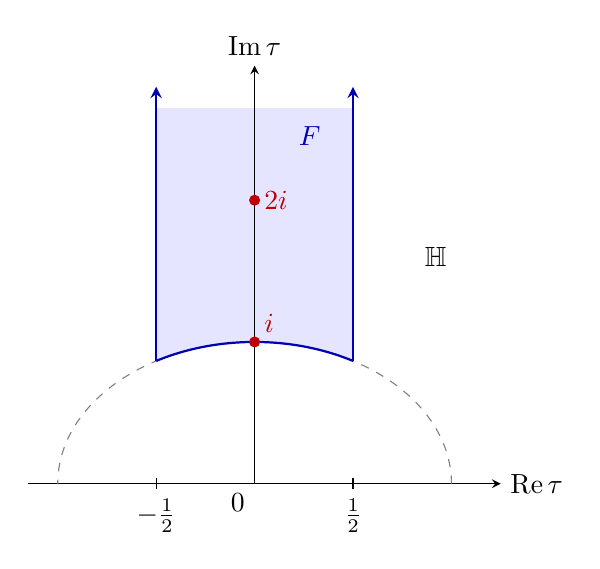
\begin{tikzpicture}[x=2.5cm,y=1.8cm,>=stealth]
  % 基本領域（上方は省略）
  \fill[blue!10]
    (-0.5,2.65)
    -- (-0.5,{sqrt(3)/2})
    arc[start angle=120,end angle=60,radius=1]
    -- (0.5,2.65)
    -- cycle;

  % 座標軸
  \draw[->] (-1.15,0)--(1.25,0)
    node[right] {$\operatorname{Re}\tau$};
  \draw[->] (0,0)--(0,2.95)
    node[above] {$\operatorname{Im}\tau$};

  % 単位半円
  \draw[gray,dashed]
    (1,0) arc[start angle=0,end angle=180,radius=1];

  % 基本領域の境界
  \draw[blue!70!black,thick,->]
    (-0.5,{sqrt(3)/2})--(-0.5,2.8);
  \draw[blue!70!black,thick,->]
    (0.5,{sqrt(3)/2})--(0.5,2.8);
  \draw[blue!70!black,thick]
    (-0.5,{sqrt(3)/2})
    arc[start angle=120,end angle=60,radius=1];

  % 目盛り
  \draw (-0.5,0.04)--(-0.5,-0.04)
    node[below] {$-\frac12$};
  \draw (0.5,0.04)--(0.5,-0.04)
    node[below] {$\frac12$};
  \node[below left] at (0,0) {$0$};

  % 二つの異なる複素構造
  \fill[red!75!black] (0,1) circle (2pt);
  \node[red!75!black,above right] at (0,1) {$i$};

  \fill[red!75!black] (0,2) circle (2pt);
  \node[red!75!black,right] at (0,2) {$2i$};

  % 領域の名前
  \node[blue!70!black] at (0.28,2.45) {$F$};
  \node at (0.92,1.6) {$\mathbb H$};
\end{tikzpicture}

{\small
青い領域は基本領域 $F$ を表し, 上方へ無限に続く.
境界の点は上記の規則で同一視する.
}
\end{center}

例えば, 図の二点 $i,2i$ が定める曲面$E_i, E_{2i}$は$C^\infty$ 級微分同相であるが, 双正則同型ではない.
\end{rem}



\subsection{種数 $2$ のコンパクトRiemann 面の構造}\label{O-S064}

\begin{prop}[次数 $1$ の因子による判定]\label{O-M361}
$X$ 上に
\[
\deg D=1,\qquad
\dim_{\mathbb C}H^0(X,\mathcal O_X(D))\geq2
\]
を満たす因子 $D$ が存在するとする.
このとき, 
\[
\dim_{\mathbb C}H^0(X,\mathcal O_X(D))=2
\]
であり, $|D|$ は基点自由である.
さらに, 
\[
\Phi_{|D|}:X\longrightarrow\C\mathbb P^1
\]
は双正則同型である.
\end{prop}
\begin{proof}
零でない切断が存在するので,
$D$ は次数 $1$ の効果的因子, すなわち一点 $p$ と線形同値である
（補題\ref{lem-complete-linear-system}参照）.
従って, $D=p$ としてよい
（補足\ref{O-M328}参照）.

補題\ref{O-M332}より, 一点の極を許しても切断の次元は
高々 $1$ しか増えないので,
\[
2\leq h^0(\mathcal O_X(p))
\underalign{\text{(補題\ref{O-M332})}}{\leq}
\underbrace{h^0(\mathcal O_X)}_{=1\ \text{(系\ref{O-M067})}}+1=2.
\]
従って, $h^0(\mathcal O_X(D))=2$ である.

任意の二点 $q,r\in X$（$q=r$ も含む）に対して,
$\deg(D-q-r)=-1$ なので,
\[
h^0(\mathcal O_X(D-q-r))
\underalign{\text{(補題\ref{O-M294})}}{=}0
=h^0(\mathcal O_X(D))-2.
\]
従って, 埋め込み判定法\ref{O-M346}より,
$|D|$ は基点自由であり,
$\Phi_{|D|}:X\to\C\mathbb P^1$ は正則埋め込みである.
さらに, 定理\ref{O-M066}より全射なので,
双正則同型である.
\end{proof}

次に, 次数 $2$ の因子を考える.

\begin{thm}[次数 $2$ の因子と超楕円曲線]
\label{O-M362}\label{O-M363}
$X$ を種数 $g\geq1$ のコンパクトRiemann 面とする.
次の三つは同値である.

\medskip
\noindent
\textbf{(1)}
次数 $2$ の因子 $D$ で,
$\dim_\C H^0(X,\mathcal O_X(D))\geq2$ となるものが存在する.

\medskip
\noindent
\textbf{(2)}
次数 $2$ の正則写像 $x:X\to\C\mathbb P^1$ が存在する.

\medskip
\noindent
\textbf{(3)}
相異なる複素数 $a_1,\ldots,a_{2g+2}$ が存在して,
$X$ は
\begin{equation}\label{O-EQ128}
y^2=\prod_{i=1}^{2g+2}(x-a_i)
\end{equation}
のコンパクト化と双正則同型である.
つまり定義\ref{O-M166}の超楕円曲線と同型である. 
\end{thm}

\begin{proof}
\textbf{(1)$\Rightarrow$(2)：二つの切断から二重被覆を作る.}

任意の点 $p\in X$ に対して $\deg(D-p)=1$ である.
$g\geq1$ なので, 命題\ref{O-M361}より
$h^0(\mathcal O_X(D-p))\leq1$ である.
従って,
\[
2\leq h^0(\mathcal O_X(D))
\underalign{\text{(補題\ref{O-M332})}}{\leq}
\underbrace{h^0(\mathcal O_X(D-p))}_{\leq1}+1
\leq2.
\]
すべて等号なので,
\begin{equation}\label{O-EQ127}
h^0(\mathcal O_X(D))=2,\qquad
h^0(\mathcal O_X(D-p))=1.
\end{equation}
これはすべての $p$ で成り立つから,
補題\ref{O-M332}より $|D|$ は基点自由である.

零でない切断があるので,
$D$ を線形同値な効果的因子 $p+q$ に置き換えてよい.
ただし $p=q$ も許す
（補題\ref{lem-complete-linear-system},
補足\ref{O-M328}参照）.
このとき, 切断の基底を $1,x$ と取れる.
$x$ は非定数で, 極の位数の総和は高々 $2$ なので,
\[
1\leq\deg x
\underalign{\text{(定理\ref{O-M071})}}{=}
\sum_{r\in x^{-1}(\infty)}
\underbrace{-\operatorname{ord}_r(x)}_{\text{極の位数}}
\leq2.
\]
次数が $1$ ならば, 系\ref{O-M074}より
$X\simeq\C\mathbb P^1$ となり, $g\geq1$ に反する.
従って $\deg x=2$ である.
基底 $1,x$ による写像は $\Phi_{|D|}=[1:x]$ なので,
$\Phi_{|D|}$ の次数も $2$ である.

\medskip
\noindent
\textbf{分岐点の個数.}

次数 $2$ の写像では, 分岐点の分岐指数はすべて $2$ である.
分岐点の個数を $b$ とすると,
\[
2g-2
\underalign{\text{(Hurwitzの公式, 定理\ref{O-M306})}}{=}
2\underbrace{\bigl(2g(\C\mathbb P^1)-2\bigr)}_{=-2}
+b(2-1)
=-4+b.
\]
従って $b=2g+2$ である.
また, 一つの分岐点だけでファイバーの重複度の和が $2$ になるため,
異なる分岐点が同じ点に移ることはない
（定理\ref{O-M071}参照）.

\medskip
\noindent
\textbf{(2)$\Rightarrow$(3)：二次拡大を方程式で表す.}

$\infty$ が分岐値にならないように,
終域 $\C\mathbb P^1$ の座標を選ぶ.
このとき, $x$ は $\infty$ の逆像の二点で,
それぞれ単純極をもつ.

定理\ref{O-M274}より,
\[
[\mathcal M(X):\C(x)]=2.
\]
従って, ある $h\in\mathcal M(X)$ と $b(x),c(x)\in\C(x)$ により,
\[
\mathcal M(X)=\C(x,h),\qquad
h^2+b(x)h+c(x)=0
\]
と書ける.
平方完成して $y_0:=h+b(x)/2$ とおけば,
\[
y_0^2=\frac{b(x)^2}{4}-c(x)=:R(x),
\qquad
\mathcal M(X)=\C(x,y_0).
\]
$R(x)$ が $\C(x)$ の元の平方ならば
$y_0\in\C(x)$ となり, 拡大次数が $2$ であることに反する.

$R(x)$ から平方因子を取り除くと,
ある $q(x)\in\C(x)\setminus\{0\}$ と
モニックで重根をもたない多項式 $P(x)$ によって,
\[
R(x)=q(x)^2P(x)
\]
と書ける.
\footnote{
$R(x)=c\prod_j(x-b_j)^{m_j}$ と分解し,
$m_j=2n_j+\varepsilon_j$,
$\varepsilon_j\in\{0,1\}$ と書けばよい.
$c$ の平方根も $q(x)$ に含める.
負の $m_j$ についても同じ分解ができる.
}
そこで $y:=y_0/q(x)$ とおくと,
\[
\mathcal M(X)=\C(x,y),\qquad y^2=P(x)
\]
となる.

$k:=\deg P$ とする.
$x$ の単純極 $p$ では,
\[
2\operatorname{ord}_p(y)
=\operatorname{ord}_p(P(x))
=k\underbrace{\operatorname{ord}_p(x)}_{=-1}
=-k.
\]
従って $k$ は偶数である.
また, $P$ が定数ならば $R$ は平方になってしまうので,
$k=2r\geq2$ と書ける.

ここで, \ref{O-S029}節の方法で
$y^2=P(x)$ をコンパクト化した曲面を $C$ とする.
例\ref{O-M280}より,
\[
\mathcal M(C)\simeq
\C(x)[T]/(T^2-P(x))
\simeq\mathcal M(X).
\]
最後の同型では, $T$ の剰余類を $y\in\mathcal M(X)$ に送る.
従って,
\[
X
\underalign{\text{(定理\ref{thm-function-field-determines-surface})}}{\simeq}
C.
\]
これにより, 写像を局所座標で構成し直すことなく,
二つの曲面が双正則同型であると分かる.

$P$ の次数は $2r$ なので, 例\ref{O-M311}より
$g(C)=r-1$ である.
従って $g=r-1$, すなわち $\deg P=2g+2$ であり,
\eqref{O-EQ128}の表示を得る.

\medskip
\noindent
\textbf{(3)$\Rightarrow$(1)：無限遠点で極を許す.}

\ref{O-S029}節の構成より,
$x$ は二つの無限遠点 $p_\infty^+,p_\infty^-$ に
それぞれ単純極をもち, ほかには極をもたない.
従って,
\[
D:=p_\infty^++p_\infty^-,
\qquad
1,x\in H^0(X,\mathcal O_X(D))
\]
と取れる.
$1,x$ は一次独立なので,
$\deg D=2$ かつ $h^0(\mathcal O_X(D))\geq2$ である.
以上で証明が完了した.
\end{proof}



\begin{cor}[種数 $2$ のRiemann 面は超楕円曲線である]
\label{cor-genus-two-hyperelliptic}
種数 $2$ のコンパクトRiemann 面 $X$ は超楕円曲線である.
より詳しく, 標準一次系 $|K_X|$ は基点自由であり, 
標準写像
\[
\Phi_{|K_X|}:X\longrightarrow\C\mathbb P^1
\]
は, 異なる六点を分岐値とする二重被覆である.

従って, $X$ は互いに異なる六つの複素数
$a_1,\ldots,a_6$ を用いて
\[
y^2=(x-a_1)\cdots(x-a_6)
\]
と表される超楕円曲線と双正則同型になる.
\end{cor}

\begin{proof}
系 \ref{O-M298} より, 
\[
\deg K_X=2g-2=2,\qquad
\dim_{\mathbb C}H^0(X,\mathcal O_X(K_X))=g=2.
\]
従って, $D=K_X$ に定理\ref{O-M362} を適用すればよい.
\end{proof}



\subsection{標準写像と超楕円曲線}\label{O-S065}

これまでは, 因子 $D$ を選ぶことで
射影空間への写像を作ってきた.
ここでは, 標準因子 $K_X$ に付随する写像を考える.

\begin{dfn}[標準写像]\label{O-M364}

$X$ を種数 $g\geq2$ のコンパクトRiemann 面とする.
標準因子 $K_X$ に付随する写像
\[
\Phi_{|K_X|}:X\dashrightarrow\C\mathbb P^{g-1}
\]
を, $X$ の標準写像という.

補題\ref{O-M286}より, $H^0(X,\Omega_X^1)$ の基底を
$\omega_j=h_j(z)\,dz$ と局所表示すれば,
\[
\Phi_{|K_X|}(p)=[h_0(p):\cdots:h_{g-1}(p)]
\]
である. ここではすべての係数が同時に零となる点を除いて表示する.
\end{dfn}

後で示すように, $|K_X|$ は基点自由である.
従って, 上の表示はすべての点で意味をもち, 
標準写像は $X$ 全体で正則となる.

その像を説明するため, 
$\C\mathbb P^1$ の基本的な射影埋め込みを導入する.

\begin{dfn}[Veronese埋め込み]\label{O-M353}
正の整数 $d$ に対して, 次数 $d$ の単項式を並べた写像
\[
\nu_d:\C\mathbb P^1\longrightarrow\C\mathbb P^d,
\qquad
[s:t]\longmapsto[s^d:s^{d-1}t:\cdots:st^{d-1}:t^d]
\]
を, 次数 $d$ のVeronese埋め込みという.
この写像が正則埋め込みであることは, 次の例で確認する.

その像 $C_d:=\nu_d(\C\mathbb P^1)$ を,
次数 $d$ のVeronese曲線という.
特に, $C_3\subset\C\mathbb P^3$ をねじれ三次曲線という.
\end{dfn}

例えば, $d=2,3$ の場合は,
\[
\nu_2([s:t])=[s^2:st:t^2],\qquad
\nu_3([s:t])=[s^3:s^2t:st^2:t^3]
\]
である.
以下では, この写像が切断の基底 $1,z,\ldots,z^d$ から
得られることを確認する.

\begin{exa}[$\C\mathbb P^1$ 上の因子とVeronese埋め込み]
\label{O-M352}
$\C\mathbb P^1$ 上の次数 $d\geq1$ の因子 $D$ に対して,
付随する写像 $\Phi_{|D|}$ は,
終域の射影変換の違いを除いて $\nu_d$ に一致する.
特に, $\nu_d$ は正則埋め込みであり,
$C_d\simeq\C\mathbb P^1$ である.
\end{exa}

\begin{proof}
\textbf{(1) $D=d[\infty]$ の場合.}

定義\ref{O-M199}より,
$H^0(\C\mathbb P^1,\mathcal O_{\C\mathbb P^1}(d[\infty]))$ は,
$\infty$ にのみ高々 $d$ 位の極を許す有理型関数の空間である.
命題\ref{O-M022}より, これらは有理関数である.
有限の点に極がないので多項式であり,
$\infty$ での極の位数はその次数に等しい.
従って,
\[
H^0(\C\mathbb P^1,\mathcal O_{\C\mathbb P^1}(d[\infty]))
=\operatorname{span}_{\C}\{1,z,\ldots,z^d\}.
\]
この基底から得られる写像は, 有限部分では
\begin{equation}\label{O-EQ113}
z\longmapsto[1:z:\cdots:z^d]
\end{equation}
である.
$z=t/s$ を代入すると,
\[
[1:t/s:\cdots:(t/s)^d]
\underalign{\text{(全成分に $s^d$ を掛ける)}}{=}
[s^d:s^{d-1}t:\cdots:t^d].
\]
右辺は $s=0$ でも定まり,
無限遠点 $[0:1]$ を $[0:\cdots:0:1]$ に送る.
従って, この写像は $\nu_d$ である.

また, $g(\C\mathbb P^1)=0$ なので,
$d\geq1=2g+1$ である.
埋め込み定理\ref{O-M333}より, $\nu_d$ は正則埋め込みとなる.

\medskip
\noindent
\textbf{(2) 一般の次数 $d$ の因子の場合.}

$D=\sum_i n_i[a_i]+n_\infty[\infty]$ と書く.
各因子 $z-a_i$ は $a_i$ に単純零点,
$\infty$ に単純極をもつので,
\[
\operatorname{div}\left(\prod_i(z-a_i)^{n_i}\right)
=\sum_i n_i[a_i]
-\underbrace{\left(\sum_i n_i\right)}_{=d-n_\infty}[\infty]
=D-d[\infty].
\]
従って, $D\sim d[\infty]$ である.
線形同値な因子は対応する基底のもとで同じ写像を与え,
基底の変更は終域の射影変換に対応する
（補足\ref{O-M328}参照）.
よって, 一般の $D$ についても結論が成り立つ.
\end{proof}


\begin{exa}[Veronese曲線の方程式]\label{O-M354}
$d=1$ の場合は $\nu_1=\mathrm{id}_{\C\mathbb P^1}$ である.

$d=2$ の場合は
\[
\nu_2([s:t])=[s^2:st:t^2]
\]
であり, その像は非特異二次曲線
\[
C_2=\{X_0X_2-X_1^2=0\}\subset\C\mathbb P^2
\]
である.

$d=3$ の場合は
\[
\nu_3([s:t])=[s^3:s^2t:st^2:t^3]
\]
であり, その像は
\[
C_3=
\left\{
\begin{aligned}
X_0X_2-X_1^2&=0,\\
X_0X_3-X_1X_2&=0,\\
X_1X_3-X_2^2&=0
\end{aligned}
\right\}
\subset\C\mathbb P^3
\]
である.

一般に, $C_d$ は
\begin{equation}\label{O-EQ114}
\operatorname{rank}
\begin{pmatrix}
X_0&X_1&\cdots&X_{d-1}\\
X_1&X_2&\cdots&X_d
\end{pmatrix}
=1
\end{equation}
で定まる.
すなわち, この行列のすべての $2\times2$ 小行列式を
零とした共通零点集合である.

また, 超平面の方程式を $\nu_d$ で引き戻すと, 
$s,t$ の $d$ 次同次式になる.
従って, $C_d$ の次数は $d$ である.
\end{exa}

これを用いると, 標準写像の構造は次のように記述できる.

\begin{thm}[標準写像と超楕円曲線]\label{O-M365}
$X$ を種数 $g\geq2$ のコンパクトRiemann 面とする.
標準一次系 $|K_X|$ は基点自由であり,
標準写像
\[
\Phi_{|K_X|}:X\longrightarrow\C\mathbb P^{g-1}
\]
は正則写像である.
この写像の形は, 次の二つに分かれる.

\medskip
\noindent
\textbf{(1) $X$ が超楕円曲線でない場合.}
$\Phi_{|K_X|}$ は正則埋め込みである.

\medskip
\noindent
\textbf{(2) $X$ が超楕円曲線である場合.}
適切な射影座標を選ぶと,
\[
\Phi_{|K_X|}=\nu_{g-1}\circ\pi,\qquad
X\xrightarrow{\ \pi\ }\C\mathbb P^1
\xrightarrow{\ \nu_{g-1}\ }\C\mathbb P^{g-1}
\]
と分解される.
ここで $\pi$ は次数 $2$ の正則写像,
$\nu_{g-1}$ は次数 $g-1$ のVeronese埋め込みである.
従って, 標準写像の像はVeronese曲線 $C_{g-1}$ であり,
$X\to C_{g-1}$ は, 異なる $2g+2$ 個の分岐値をもつ二重被覆である.
特に, 標準写像は埋め込みではない.

\medskip
いずれの場合も $3K_X$ は非常に豊富であり,
$\Phi_{|3K_X|}$ は正則埋め込みを与える.
\end{thm}

\begin{proof}
\textbf{(1) 各点で零にならない正則 $1$ 形式が存在する.}

$p\in X$ を取る.
定数関数は $\mathcal O_X(p)$ の切断なので,
$h^0(\mathcal O_X(p))\geq1$ である.
もし次元が $2$ 以上ならば, 命題\ref{O-M361}より
$X\simeq\C\mathbb P^1$ となり, $g\geq2$ に反する.
従って, $h^0(\mathcal O_X(p))=1$ である.

Riemann--Rochの公式を $p$ に適用すると,
\begin{equation}\label{O-EQ129}
h^0(\mathcal O_X(K_X-p))
\underalign{\text{(系\ref{O-M297})}}{=}
\underbrace{h^0(\mathcal O_X(p))}_{=1}+g-2
=g-1.
\end{equation}
一方, $h^0(\mathcal O_X(K_X))=g$ である
（系\ref{O-M298}参照）.
従って, 各点を引くと次元がちょうど $1$ 減るので,
補題\ref{O-M332}より $|K_X|$ は基点自由である.

これは, 各点で零にならない正則 $1$ 形式が存在することを意味する
（補題\ref{O-M286}参照）.
よって, 標準写像は $X$ 全体で正則に定まる.

\medskip
\noindent
\textbf{(2) 超楕円曲線でない場合は, 埋め込み判定法を使う.}

$X$ が超楕円曲線でないとする.
任意の二点 $p,q\in X$（$p=q$ も含む）に対して,
\[
h^0(\mathcal O_X(p+q))=1
\]
である.
実際, 定数関数が切断を与えるので次元は $1$ 以上であり,
$2$ 以上ならば定理\ref{O-M362}より超楕円曲線になってしまう.

従って,
\begin{equation}\label{O-EQ130}
h^0(\mathcal O_X(K_X-p-q))
\underalign{\text{(系\ref{O-M297})}}{=}
\underbrace{h^0(\mathcal O_X(p+q))}_{=1}+g-3
=g-2.
\end{equation}
つまり, 任意の二点を引くと切断の次元がちょうど $2$ 減る.
命題\ref{O-M346}の埋め込み判定法より,
$\Phi_{|K_X|}$ は正則埋め込みである.

\medskip
\noindent
\textbf{(3) 超楕円曲線の場合は, 標準写像を具体的に書く.}

定理\ref{O-M362}より, $X$ を
\[
y^2=\prod_{j=1}^{2g+2}(x-a_j)
\]
のコンパクト化として表す.
例\ref{O-M311}に続く補足より,
\[
\frac{dx}{y},\quad
x\frac{dx}{y},\quad\ldots,\quad
x^{g-1}\frac{dx}{y}
\]
は $H^0(X,\Omega_X^1)$ の基底である.

$K_X=\operatorname{div}(dx/y)$ と取ると,
補題\ref{O-M286}の同型
\[
H^0(X,\mathcal O_X(K_X))
\xrightarrow{\sim}H^0(X,\Omega_X^1),
\qquad
\varphi\longmapsto\varphi\frac{dx}{y}
\]
によって, $1,x,\ldots,x^{g-1}$ が
$H^0(X,\mathcal O_X(K_X))$ の基底となる.
従って, $x$ が有限のところでは,
\[
\Phi_{|K_X|}(p)
=[1:x(p):\cdots:x(p)^{g-1}]
\underalign{\text{(定義\ref{O-M353})}}{=}
\nu_{g-1}\bigl([1:x(p)]\bigr).
\]

$\pi:X\to\C\mathbb P^1$ を $x$ が定める二重被覆とすると,
これは $\Phi_{|K_X|}=\nu_{g-1}\circ\pi$ を意味する.
両辺は全体で正則なので, 無限遠点でも連続性により一致する.

$\nu_{g-1}$ は正則埋め込みだから,
標準写像の像は $C_{g-1}$ であり,
像への写像は $\pi$ と同じ二重被覆である
（例\ref{O-M352}参照）.
その分岐値は $2g+2$ 個である
（定理\ref{O-M362}参照）.

\medskip
\noindent
\textbf{(4) $3K_X$ は常に埋め込みを与える.}

$g\geq2$ より,
\[
\deg(3K_X)
\underalign{\text{(系\ref{O-M298})}}{=}
6g-6
=2g+1+\underbrace{(4g-7)}_{\geq1}
\geq2g+1.
\]
従って, 埋め込み定理\ref{O-M333}より,
$3K_X$ は非常に豊富である.
\end{proof}


\subsection{高次元の場合の標準写像-Hacon--McKernan・Takayama・Tsujiの定理-}
\label{sec-higher-dimensional-canonical-map}

曲線では $3K_X$ が埋め込みを与えることを示した（定理\ref{O-M365}）. 高次元でも標準因子の倍数を考えると, 次元だけに依存する倍数で双有理写像を得られる.
$X$ を $n$ 次元の非特異複素射影多様体とし,
$K_X$ を標準束 $\bigwedge^n\Omega_X^1$ に対応する標準因子とする.
\[
H^0(X,\mathcal O_X(mK_X))\neq0
\]
のとき, この空間の基底から定まる有理写像
\[
\Phi_{|mK_X|}:X\dashrightarrow\C\mathbb P^{N_m},
\qquad
N_m=\dim_{\mathbb C}H^0(X,\mathcal O_X(mK_X))-1
\]
を $m$ 重標準写像という.

\begin{thm}[多重標準写像の一様な双有理性　(Hacon--McKernan, Takayama, Tsuji 2006--2007)]
\label{thm-uniform-pluricanonical-map}
各正の整数 $n$ に対して, 正の整数 $r_n$ が存在し,
任意の $n$ 次元の一般型非特異複素射影多様体 $X$ について,
\[
m\geq r_n
\quad\Longrightarrow\quad
\Phi_{|mK_X|}\text{ は像への双有理写像}
\]
が成り立つ.
\end{thm}
ここで重要なのは, $r_n$ を次元 $n$ だけで選べることである.
双有理であるとは, $X$ とその像の適当な稠密開集合の間で
同型を与えることをいう.
高次元では, この写像が全体で定義された埋め込みになるとは限らない.
ちなみに上の"Takayama"は高山茂晴先生のことで私の指導教官である. 

\begin{rem}[標準因子の体積との関係]
標準因子の体積を
\[
\operatorname{vol}(K_X)
:=
\limsup_{m\to\infty}
\frac{n!}{m^n}
\dim_{\mathbb C}H^0(X,\mathcal O_X(mK_X))
\]
と定める.
これは多重標準形式の空間の次元が増える速さを表す量である.
一般型の $X$ では
\[
0<\operatorname{vol}(K_X)<\infty
\]
であり, 種数 $g\geq2$ の曲線では
\[
\operatorname{vol}(K_X)=\deg K_X=2g-2
\]
となる.

定理 \ref{thm-uniform-pluricanonical-map} の帰結として,
次元 $n$ のみに依存する定数 $\varepsilon_n>0$ が存在し,
すべての $n$ 次元の一般型非特異複素射影多様体について,
\[
\operatorname{vol}(K_X)\geq\varepsilon_n
\]
が成り立つ.
つまり, 次元を固定すると, 標準因子の体積は
任意に小さくなることはない.

\end{rem}


\subsection{種数 $3$ のコンパクトRiemann 面の構造}

\begin{thm}[種数 $3$ のコンパクトRiemann 面]\label{O-M368}
種数 $3$ のコンパクトRiemann 面 $X$ は,
次のいずれか一方と双正則同型である.

\medskip
\noindent
\textbf{(1) 非超楕円曲線の場合.}
$\C\mathbb P^2$ 内の非特異四次曲線.
この曲線は, 標準写像
$\Phi_{|K_X|}:X\hookrightarrow\C\mathbb P^2$ の像として得られる.

\medskip
\noindent
\textbf{(2) 超楕円曲線の場合.}
互いに異なる八つの複素数 $a_1,\ldots,a_8$ を用いた曲線
\[
y^2=\prod_{i=1}^8(x-a_i)
\]
のコンパクト化.

\medskip
逆に, 非特異平面四次曲線は種数 $3$ の非超楕円曲線であり,
(2) の曲線は種数 $3$ の超楕円曲線である.
\end{thm}

\begin{proof}
\textbf{(1) 種数 $3$ の曲面を標準写像で分類する.}

$X$ が超楕円曲線でなければ,
定理\ref{O-M365}より標準写像は正則埋め込みである.
また,
\[
h^0(\mathcal O_X(K_X))
\underalign{\text{(系\ref{O-M298})}}{=}g(X)=3
\]
なので, その終域は $\C\mathbb P^2$ である.

像 $C:=\Phi_{|K_X|}(X)$ は,
Chowの定理\ref{O-M341}により非特異射影平面曲線である.
その次数を $m$ とすると,
\[
3=g(C)
\underalign{\text{(例\ref{O-M317})}}{=}
\frac{(m-1)(m-2)}2.
\]
整理すると $(m-4)(m+1)=0$ であり,
$m\geq1$ なので $m=4$ である.

一方, $X$ が超楕円曲線ならば,
定理\ref{O-M362}より,
$2g+2=8$ 個の異なる根をもつ方程式
$y^2=\prod_{i=1}^8(x-a_i)$ で表される.

\medskip
\noindent
\textbf{(2) 逆に, どちらの曲線も種数は $3$ である.}

非特異平面四次曲線 $C$ については,
\[
g(C)
\underalign{\text{(例\ref{O-M317})}}{=}
\frac{(4-1)(4-2)}2=3.
\]
また, 八つの異なる根をもつ超楕円曲線についても,
例\ref{O-M311}より種数は $3$ である.

\medskip
\noindent
\textbf{(3) 非特異平面四次曲線は超楕円曲線ではない.}

非特異四次曲線 $C\subset\C\mathbb P^2$ を取る.
その標準写像が, もとの平面への埋め込みになることを示す.

$X_0=0$ が $C$ と横断的に交わるように座標を選び,
交点因子を $H_C$ とする.
例\ref{O-M317}の証明で構成した有理型 $1$ 形式 $\omega$ は,
\[
\operatorname{div}(\omega)
=\underbrace{(4-3)}_{=1}H_C
=H_C
\]
を満たす.
従って, 標準因子の代表元を $K_C=H_C$ と取れる.

ここで,
\[
1,\qquad x:=\frac{X_1}{X_0},\qquad
y:=\frac{X_2}{X_0}
\]
は $H^0(C,\mathcal O_C(H_C))$ の切断である.
実際, $x,y$ の極は $X_0=0$ 上にしかなく,
横断性により各点で高々単純極である.

これらは一次独立である.
もし $a+bx+cy=0$ という非自明な関係があれば,
$C$ 全体が直線 $aX_0+bX_1+cX_2=0$ に含まれてしまうからである.
一方,
\[
\dim_{\C}H^0(C,\mathcal O_C(H_C))
=h^0(\mathcal O_C(K_C))
\underalign{\text{(系\ref{O-M298})}}{=}3.
\]
従って, $1,x,y$ はこの空間の基底である.

この基底による標準写像は, $X_0\neq0$ の部分で
\[
p\longmapsto[1:x(p):y(p)]
=[X_0(p):X_1(p):X_2(p)]
\]
となる.
両辺は全体で正則なので, この一致は無限遠点でも成り立つ.
つまり, 標準写像はもとの埋め込み
$C\hookrightarrow\C\mathbb P^2$ である.

超楕円曲線の標準写像は二重被覆であり,
埋め込みではない（定理\ref{O-M365}参照）.
従って, $C$ は超楕円曲線ではなく,
二つの場合は排他的である.
\end{proof}

\begin{rem}[四次曲線の直線切断と方程式]\label{O-M369}
$C\subset\C\mathbb P^2$ を非特異四次曲線とする.
定理\ref{O-M368}より, $g(C)=3$ であり,
もとの平面への埋め込みは標準写像である.

\medskip
\noindent
\textbf{(1) 直線との交点は, 正則 $1$ 形式の零点になる.}

直線 $H$ が $C$ と異なる四点 $p_1,\ldots,p_4$ で交わるとする.
このとき,
\[
\operatorname{div}(\omega)=p_1+\cdots+p_4
\]
となる正則 $1$ 形式 $\omega$ が存在する.

実際, 標準写像がもとの埋め込みに一致するように,
$H^0(C,\Omega_C^1)$ の基底 $\omega_0,\omega_1,\omega_2$ を選ぶ.
直線の方程式を $a_0X_0+a_1X_1+a_2X_2=0$ とし,
\[
\omega:=a_0\omega_0+a_1\omega_1+a_2\omega_2
\]
とおく.
基底の一次独立性から $\omega\neq0$ である.

局所座標 $z$ で $\omega_i=h_i(z)\,dz$ と書くと,
標準写像は $[h_0(z):h_1(z):h_2(z)]$ で表される.
従って,
\[
p\in C\cap H
\quad\Longleftrightarrow\quad
a_0h_0(p)+a_1h_1(p)+a_2h_2(p)=0
\quad\Longleftrightarrow\quad
\omega(p)=0.
\]
一方,
\[
\deg\operatorname{div}(\omega)
\underalign{\text{(系\ref{O-M298})}}{=}
2\underbrace{g(C)}_{=3}-2=4.
\]
$\omega$ は正則で, 異なる四点 $p_1,\ldots,p_4$ で零になるので,
各零点の位数はちょうど $1$ であり, 他に零点はない.

\medskip
\noindent
\textbf{(2) 四次方程式は, $15$ 個の切断の一次関係から得られる.}

$H^0(C,\mathcal O_C(K_C))$ の基底を $s_0,s_1,s_2$ とする.
これらの四次単項式
\begin{equation}\label{O-EQ132}
s_0^i s_1^j s_2^k,\qquad
i,j,k\geq0,\quad i+j+k=4
\end{equation}
は, すべて $H^0(C,\mathcal O_C(4K_C))$ の切断である.
その個数は $\binom{6}{2}=15$ 個である.

ところが, $\deg K_C=4$ なので,
\begin{equation}\label{O-EQ131}
\dim_\C H^0(C,\mathcal O_C(4K_C))
\underalign{\text{(系\ref{O-M302})}}{=}
\underbrace{\deg(4K_C)}_{=16}+1-\underbrace{g(C)}_{=3}
=14.
\end{equation}
従って, $15$ 個の切断の間には非自明な一次関係
\[
\sum_{i+j+k=4}a_{ijk}s_0^i s_1^j s_2^k=0
\]
が存在する.
ここで, 係数 $a_{ijk}$ はすべてが零ではない.

よって, 標準写像の像は非零の四次同次多項式
\[
F(X_0,X_1,X_2)
:=\sum_{i+j+k=4}a_{ijk}X_0^iX_1^jX_2^k
\]
の零点集合に含まれる.
この像は非特異四次曲線なので,
その定義多項式も既約な四次式である.
従って, $F$ はその定義多項式の零でない定数倍であり,
$F=0$ が標準曲線の方程式を与える.
\end{rem}



\subsection{コンパクトRiemann 面の三次元射影空間への埋め込み}

埋め込み定理 \ref{O-M333} により, 
コンパクトRiemann 面は十分大きな射影空間に埋め込める.
実は, 射影空間の次元は $3$ まで下げることができる.


\begin{thm}[三次元射影空間への埋め込み]\label{thm-embedding-p3}
任意のコンパクトRiemann 面 $X$ は,
$\C\mathbb P^3$ に正則に埋め込める.
\end{thm}

現時点できちんと証明をするのは難しいので概略のみ述べる. 
\begin{proof}[証明の概略]
定理\ref{O-M333}により,
まず $X\hookrightarrow\C\mathbb P^N$ と埋め込む.
$N\leq3$ ならば,
線形な包含 $\C\mathbb P^N\hookrightarrow\C\mathbb P^3$
と合成すればよい.

以下では, $N\geq4$ のとき,
埋め込みを保ったまま終域の次元を一つ下げる方法を説明する.

\medskip
\noindent
\textbf{(1) 一点を中心として射影する.}

中心 $A\in\C\mathbb P^N$ と,
$A$ を通らない超平面 $H\simeq\C\mathbb P^{N-1}$ を選ぶ.
$A$ と点 $p$ を結ぶ直線が $H$ と交わる点を $p_A(p)$ とする.
これが $A$ を中心とする射影である.

例えば $A=[1:0:\cdots:0]$, $H=\{Z_0=0\}$ とすれば,
\[
p_A:\C\mathbb P^N\setminus\{A\}
\longrightarrow\C\mathbb P^{N-1},
\qquad
[Z_0:Z_1:\cdots:Z_N]\longmapsto[Z_1:\cdots:Z_N]
\]
である.
従って, $A\notin X$ ならば,
制限 $p_A|_X$ は正則写像となる.

\begin{figure}[htbp]
\centering
\begin{tikzpicture}[
  scale=1.1,
  >=stealth,
  every node/.style={font=\small},
  point/.style={circle,fill=black,inner sep=1.7pt}
]
% 超平面 H の模式図
\filldraw[fill=blue!7,draw=blue!60!black]
  (-2,-1)--(2.8,-1)--(4,0.65)--(-0.8,0.65)--cycle;
\node[blue!60!black] at (2.7,0.15)
  {$H\simeq\C\mathbb P^{N-1}$};

% 中心, 射影する点, 像
\coordinate (A) at (-1,3);
\coordinate (P) at (0,1.4);
\coordinate (Q) at (1,-0.2);

% A と p を結ぶ直線
\draw[gray,dashed] (Q)--(1.5,-1);
\draw[red!75!black,thick] (A)--(P);
\draw[red!75!black,thick,->] (P)--(Q);

% 点とラベル
\node[point,label=above:{$A$（射影の中心）}] at (A) {};
\node[point,label=right:{$p$}] at (P) {};
\node[point,label=below left:{$p_A(p)$}] at (Q) {};

\node[red!75!black,left] at (-0.55,2.28) {直線 $Ap$};
\node at (1,-1.55) {$p_A(p)=Ap\cap H$};
\end{tikzpicture}
\label{fig-projection-from-point}
\end{figure}

\medskip
\noindent
\textbf{(2) 埋め込みを保つために, 割線と接線を避ける.}

射影によって埋め込みが壊れる原因は, 次の二つである.

\begin{figure}[htbp]
\centering
\begin{tikzpicture}[
  scale=0.9,
  every node/.style={font=\small},
  curve/.style={blue!70!black,thick},
  ray/.style={red!75!black,thick},
  point/.style={circle,fill=black,inner sep=1.6pt}
]

% 左：割線上の中心
\begin{scope}
  \node at (1.6,3.65) {割線上に中心を取った場合};

  % 射影先
  \draw[thick] (-0.45,0)--(3.9,0);
  \node[right] at (3.9,0) {$H$};

  % 曲線：p と q を通る
  \draw[curve]
    (0.25,1.65)
    .. controls (0.45,2.45) and (0.75,2.2) ..
    (1,2)
    .. controls (1.6,2.35) and (2.65,1.5) ..
    (2,1)
    .. controls (1.7,0.75) and (2.7,0.55) ..
    (3.2,0.9);
  \node[blue!70!black] at (3.4,1.05) {$X$};

  % A, p, q は一直線上
  \draw[ray] (0,3)--(3,0);
  \node[point,label=above left:{$A$}] at (0,3) {};
  \node[point,label=left:{$p$}] at (1,2) {};
  \node[point,label=right:{$q$}] at (2,1) {};
  \node[point] at (3,0) {};
  \node[below] at (2.6,-0.1) {$p_A(p)=p_A(q)$};

  \node at (1.65,-0.85) {異なる二点が重なる};
\end{scope}

% 右：接線上の中心
\begin{scope}[shift={(6,0)}]
  \node at (1.6,3.65) {接線上に中心を取った場合};

  % 射影先
  \draw[thick] (-0.45,0)--(3.9,0);
  \node[right] at (3.9,0) {$H$};

  % p で接線の傾きが -1 となる曲線
  \draw[curve]
    (0.3,1.1)
    .. controls (0.65,1.6) and (1.05,1.95) ..
    (1.5,1.5)
    .. controls (1.95,1.05) and (2.55,0.8) ..
    (3.25,1.5);
  \node[blue!70!black] at (3.45,1.6) {$X$};

  % 接線
  \draw[ray] (0,3)--(3,0);
  \node[point,label=above left:{$A$}] at (0,3) {};
  \node[point,label=above right:{$p$}] at (1.5,1.5) {};
  \node[red!75!black,right] at (0.65,2.5) {接線};
  \node[point] at (3,0) {};
  \node[below] at (3,-0.1) {$p_A(p)$};

  \node at (1.65,-0.85) {接方向が潰れ, 微分が零になる};
\end{scope}

\end{tikzpicture}
\label{fig-projection-secant-tangent}
\end{figure}

まず, 異なる二点 $p,q\in X$ が同じ点に写るのは,
$A,p,q$ が一直線上にある場合である.
従って, $A$ が $X$ のどの割線にも属さなければ,
$p_A|_X$ は単射である.

次に, $p$ で微分が零になるのは,
$X$ の $p$ における接線が $A$ を通る場合である.
従って, $A$ がどの接線にも属さなければ,
$p_A|_X$ の微分は各点で単射である.

\medskip
\noindent
\textbf{(3) 割線と接線を避ける中心が存在する.}

$X$ の割線全体の和集合の閉包を $S$ とする.
二点を近づけると割線は接線に近づくので,
$S$ はすべての接線も含む.

割線上の点を指定するには,
まず $X$ 上の二点を選び,
次にその二点を結ぶ直線上の点を選べばよい.
従って, 複素次元について
\[
\dim_{\C}S
\leq
\underbrace{1+1}_{\text{$X$ 上の二点を選ぶ}}
+
\underbrace{1}_{\text{直線上の点を選ぶ}}
=3
\]
となる.
\footnote{
厳密には, Chowの定理\ref{O-M341}により $X$ を射影代数曲線とみなし,
割線をパラメータ付ける代数的な族の次元を数える.
その像の閉包の次元は, パラメータ空間の次元を超えない.
ここではこの代数幾何学の次元評価を用いている.
}
$N\geq4$ なので $S$ は $\C\mathbb P^N$ 全体ではなく,
$A\notin S$ を選べる.
この中心からの射影は単射で, 各点の微分も単射である.
$X$ はコンパクトなので,
定義\ref{O-M128}より
\[
p_A|_X:X\hookrightarrow\C\mathbb P^{N-1}
\]
は正則埋め込みとなる.

以上の操作を繰り返せば,
終域の次元を $3$ まで下げることができる.
\end{proof}


\begin{rem}
$\C\mathbb P^2$ に非特異曲線として埋め込める場合には, 
例 \ref{O-M317} より, 種数は
\[
g=\frac{(m-1)(m-2)}2
\]
という形に限られる.
例えば, 種数 $2$ の曲面は
$\C\mathbb P^2$ には埋め込めないが, 
$\C\mathbb P^3$ には埋め込める.

また, $\C\mathbb P^3$ に埋め込めることと, 
二つの曲面の完全交叉として表されることは別の問題である.
\end{rem}


\subsection{種数 $4$ のコンパクトRiemann 面の構造}
これは気になったので調べて入れた. 多分難しいと思う. 
種数5以上もできると思うが, これ以上やっても意味ないのでここまでにしておく. 


\begin{thm}[種数 $4$ のコンパクトRiemann 面]
\label{thm-genus-four}
種数 $4$ のコンパクトRiemann 面 $X$ は,
次のいずれか一方と双正則同型である.

\medskip
\noindent
\textbf{(1) 超楕円曲線の場合.}
互いに異なる十個の複素数 $a_1,\ldots,a_{10}$ を用いた曲線
\[
y^2=\prod_{i=1}^{10}(x-a_i)
\]
のコンパクト化.

\medskip
\noindent
\textbf{(2) 非超楕円曲線の場合.}
$\C\mathbb P^3$ 内の二次曲面と三次曲面の
非特異な完全交叉曲線
\[
C=\{q_2=F_3=0\}\subset\C\mathbb P^3.
\]
この曲線は, 標準写像
$\Phi_{|K_X|}:X\hookrightarrow\C\mathbb P^3$ の像として得られる.

\medskip
逆に, (1) の曲線は種数 $4$ の超楕円曲線であり,
(2) の曲線は種数 $4$ の非超楕円曲線である.

ここで非特異な完全交叉とは,
二つの方程式が曲線を重複なく定め,
各点でその微分が一次独立となることをいう.
二次曲面そのものは, 特異点をもっていてもよい.
\end{thm}

\begin{proof}
超楕円曲線についての主張は,
定理\ref{O-M362}と例\ref{O-M311}から従う.
以下では, 非超楕円曲線の場合を示す.

\medskip
\noindent
\textbf{(1) 標準写像の像は, 次数 $6$ の空間曲線である.}

$g(X)=4$ なので, 系\ref{O-M298}と定理\ref{O-M365}より,
標準写像は正則埋め込み
\[
\Phi_{|K_X|}:X\hookrightarrow\C\mathbb P^3
\]
を与える.
その像を $C$ とする.

超平面の方程式を標準写像で引き戻すと,
標準束の切断が得られる.
従って, 超平面と $C$ の交点数は標準因子の次数に等しく,
\[
\deg C=\deg K_X
\underalign{\text{(系\ref{O-M298})}}{=}2\cdot4-2=6.
\]

また, 標準写像を定める基底を $s_0,s_1,s_2,s_3$ とすると,
$C$ が平面 $a_0Z_0+\cdots+a_3Z_3=0$ に含まれることは,
$a_0s_0+\cdots+a_3s_3=0$ を意味する.
基底は一次独立なので, $C$ はどの平面にも含まれない.

\medskip
\noindent
\textbf{(2) $C$ を含む二次曲面を見つける.}

二次単項式 $s_is_j$（$0\leq i\leq j\leq3$）は
$\binom{5}{2}=10$ 個あり,
すべて $H^0(X,\mathcal O_X(2K_X))$ に属する.
一方,
\[
h^0(\mathcal O_X(2K_X))
\underalign{\text{(系\ref{O-M302})}}{=}
\underbrace{\deg(2K_X)}_{=12}+1-4=9.
\]
従って, 十個の切断の間には非自明な一次関係がある.
つまり, 非零の二次同次多項式 $q_2$ が存在して,
\[
q_2(s_0,s_1,s_2,s_3)=0,
\qquad C\subset\{q_2=0\}
\]
となる.

この $q_2$ は既約である.
実際, 二つの一次式の積ならば,
既約な曲線 $C$ は一方の平面に含まれてしまい,
(1) に反する.

\medskip
\noindent
\textbf{(3) もう一つ, 独立な三次方程式を見つける.}

三次単項式 $s_0^{i_0}\cdots s_3^{i_3}$,
$i_0+\cdots+i_3=3$ は $\binom{6}{3}=20$ 個ある.
一方,
\[
h^0(\mathcal O_X(3K_X))
\underalign{\text{(系\ref{O-M302})}}{=}
\underbrace{\deg(3K_X)}_{=18}+1-4=15.
\]
従って, $C$ 上で零になる三次式の空間の次元は,
少なくとも $20-15=5$ である.

ところが, 二次式 $q_2$ から作られる三次式
\[
q_2Z_0,\quad q_2Z_1,\quad q_2Z_2,\quad q_2Z_3
\]
が張る空間は四次元である.
従って, $q_2$ の倍数ではない三次式 $F_3$ で,
$C$ 上零になるものを選べる.
こうして,
\[
C\subset\{q_2=F_3=0\}
\]
を得る.

$q_2$ は既約で, $F_3$ はその倍数ではないので,
二つの曲面は共通の曲面成分をもたない.
Bézoutの定理より, 交叉曲線の次数は
\[
\deg\{q_2=F_3=0\}
\underalign{\text{(Bézoutの定理)}}{=}2\cdot3
=6=\deg C.
\]
すでに $C$ だけで次数 $6$ を占めるため,
余分な曲線成分や $C$ の重複は存在しない.
従って, この完全交叉は $C$ に一致する.
\footnote{
厳密には, 共通の曲面成分をもたない二つの曲面の完全交叉には,
孤立した点成分や埋め込まれた点成分がないという事実も用いる.
この性質と次数の一致により,
単なる集合としてだけでなく, 重複も含めて $C$ と一致する.
}

\medskip
\noindent
\textbf{(4) 逆に, 非特異な $(2,3)$ 完全交叉の種数は $4$ である.}

$C=\{q_2=F_3=0\}\subset\C\mathbb P^3$ を
非特異な完全交叉曲線とし,
超平面との交点因子を $H_C$ とする.
Bézoutの定理と随伴公式より,
\[
\deg H_C=2\cdot3=6,\qquad
K_C\sim\underbrace{(2+3-4)}_{=1}H_C=H_C.
\]
\footnote{
$\C\mathbb P^3$ 内の次数 $a,b$ の曲面の
非特異完全交叉曲線では,
$K_C\sim(a+b-4)H_C$ が成り立つ.
これを随伴公式という.
また, 正の次数の二つの曲面の完全交叉曲線は連結である.
ここではこれらの代数幾何学の事実の証明を省略する.
}
従って,
\[
2g(C)-2
\underalign{\text{(系\ref{O-M298})}}{=}
\deg K_C=\deg H_C=6,
\]
すなわち $g(C)=4$ である.

最後に, この曲線の標準写像がもとの埋め込みになることを確認する.
$C$ は平面に含まれない.
もし含まれれば非特異平面六次曲線となり,
例\ref{O-M317}より種数が $10$ となってしまうからである.

従って, 四つの座標 $Z_0,Z_1,Z_2,Z_3$ を制限して得られる
$\mathcal O_C(H_C)$ の切断は一次独立である.
また,
\[
h^0(\mathcal O_C(H_C))
=h^0(\mathcal O_C(K_C))
\underalign{\text{(系\ref{O-M298})}}{=}4.
\]
よって, この四つの切断は基底となり,
標準写像はもとの埋め込み
$C\hookrightarrow\C\mathbb P^3$ に一致する.
従って, 定理\ref{O-M365}より $C$ は非超楕円曲線である.
\end{proof}



\newpage
\section{自己同型群}
最後に自己同型群に関して調べておこう. 特に種数が2以上ならば自己同型群が有限であることを示す. 
これは高次元の場合も拡張することができる. 

\subsection{種数 $0,1$ の自己同型群}

\begin{dfn}[自己同型群]
コンパクトRiemann 面 $X$ の双正則自己写像全体を
\(
\operatorname{Aut}(X)
\)
と書く.写像の合成を演算として群をなす.

また, $p\in X$ に対して
\[
\operatorname{Aut}(X,p)
:=
\{\sigma\in\operatorname{Aut}(X)\mid\sigma(p)=p\}
\]
を, $p$ を固定する自己同型群という.
\end{dfn}

\begin{prop}[種数 $0$ の自己同型群]\label{prop-aut-genus-zero}
種数 $0$ のコンパクトRiemann 面は $\C\mathbb P^1$ と同型であり, 
\[
\operatorname{Aut}(\C\mathbb P^1)
=\operatorname{PGL}_2(\mathbb C).
\]
すなわち, 自己同型はちょうど一次分数変換
\[
z\longmapsto\frac{az+b}{cz+d},
\qquad ad-bc\neq0
\]
である.
\end{prop}
\begin{proof}
命題\ref{O-M351}より, 種数 $0$ のコンパクトRiemann 面は
$\C\mathbb P^1$ と双正則同型である.
また, 定理\ref{thm-aut-projective-line}より,
$\C\mathbb P^1$ の自己同型はちょうど一次分数変換である.

一次分数変換の合成は対応する可逆行列の積に一致し,
二つの行列が同じ変換を定めるのは,
互いに零でない定数倍であるときに限る.
従って,
\[
\operatorname{Aut}(\C\mathbb P^1)
\simeq\operatorname{GL}_2(\C)/\{\lambda I\mid\lambda\in\C^\times\}
=\operatorname{PGL}_2(\C).
\]
\end{proof}


\begin{thm}[種数 $1$ の自己同型群]\label{thm-aut-genus-one}
$E=\C/\Lambda$ を一次元複素トーラスとする.
$E$ の自己同型は, すべて
\[
[z]\longmapsto[\alpha z]+\beta,
\qquad
\beta\in E,\quad
\alpha\in U_\Lambda
:=\{\alpha\in\C^\times\mid\alpha\Lambda=\Lambda\}
\]
と一意に書ける.
すなわち, 自己同型は格子を保つ回転と平行移動の合成である.

特に, 原点を固定する自己同型群は $U_\Lambda$ と同型であり,
$\zeta:=e^{\pi i/3}$ とおくと, 次のように分類される.
\[
\begin{array}{c|c|c}
\Lambda\text{ の形} & U_\Lambda & |U_\Lambda|\\ \hline
\lambda(\Z+i\Z)\quad(\lambda\neq0)
& \{1,i,-1,-i\} & 4\\[3pt]
\lambda(\Z+\Z\zeta)\quad(\lambda\neq0)
& \{1,\zeta,\ldots,\zeta^5\} & 6\\[3pt]
\text{上のいずれでもない場合}
& \{1,-1\} & 2
\end{array}
\]
第一の場合を正方格子と相似,
第二の場合を正三角格子と相似という.
ここで相似とは, 非零の複素数倍で移り合うことを意味する.

自己同型群全体は
\[
\operatorname{Aut}(E)\simeq E\rtimes U_\Lambda
\]
であり, 平行移動を含むため無限群である.
ここで半直積 $E\rtimes U_\Lambda$ とは,
集合 $E\times U_\Lambda$ に積
\[
(\beta,\alpha)(\beta',\alpha')
=(\beta+\alpha\beta',\alpha\alpha')
\]
を入れた群である.
これは, 対 $(\beta,\alpha)$ を写像
$[z]\mapsto[\alpha z]+\beta$ に対応させたときの合成則である.

\end{thm}


\begin{proof}
\textbf{(1) 自己同型群が半直積になることを示す.}

示すことは二つである.
まず, 自己同型が対 $(\beta,\alpha)\in E\times U_\Lambda$ と
一対一に対応することを示す.
次に, 自己同型の合成をこの対で表すと,
半直積の積になることを確認する.

\medskip
\noindent
\textbf{自己同型の形を求める.}
商写像を $p:\C\to E$ とする.
$\C$ は単連結なので,
$\varphi\in\operatorname{Aut}(E)$ に対して,
\[
p\circ\widetilde\varphi=\varphi\circ p
\]
を満たす持ち上げ $\widetilde\varphi:\C\to\C$ が存在する.
$p$ は局所双正則なので, $\widetilde\varphi$ も正則である.

$\lambda\in\Lambda$ に対して $p(z+\lambda)=p(z)$ だから,
\[
\widetilde\varphi(z+\lambda)-\widetilde\varphi(z)\in\Lambda.
\]
左辺は連続で, 値は離散集合 $\Lambda$ に属するため,
$z$ によらず一定である.
微分すると,
\[
\widetilde\varphi'(z+\lambda)=\widetilde\varphi'(z).
\]
従って, $\widetilde\varphi'$ は $E$ 上の正則関数を定める.
系\ref{O-M067}よりこれは定数なので,
\[
\widetilde\varphi(z)=\alpha z+b
\qquad(\alpha\neq0)
\]
と書ける.
ここで $\alpha=0$ ならば $\varphi$ が定値になるため,
$\alpha\neq0$ である.

この表示が格子を保つことも確認する.
任意の $\lambda\in\Lambda$ に対して,
\[
\alpha\lambda
=\widetilde\varphi(z+\lambda)-\widetilde\varphi(z)\in\Lambda
\]
なので, $\alpha\Lambda\subset\Lambda$ である.
逆に, $\mu\in\Lambda$ ならば,
\[
\varphi([\mu/\alpha])=[\mu+b]=[b]=\varphi([0]).
\]
$\varphi$ は単射なので $[\mu/\alpha]=[0]$,
すなわち $\mu\in\alpha\Lambda$ である.
従って, $\alpha\Lambda=\Lambda$ を得る.

逆に, $\alpha\in U_\Lambda$ と $\beta=[b]\in E$ に対して,
\[
\varphi_{\beta,\alpha}([z]):=[\alpha z+b]
\]
は代表元によらず定まり,
$[z]\mapsto[(z-b)/\alpha]$ を逆写像にもつ.
従って, これは自己同型である.

また, $\beta=\varphi([0])$ であり,
$\alpha$ は持ち上げの微分なので, どちらも一意に決まる.
\footnote{
同じ写像の二つの持ち上げの差は,
離散集合 $\Lambda$ に値を取る連続関数なので定数である.
従って, その微分は持ち上げの選び方によらない.
}
以上より, 対応
\[
E\times U_\Lambda\longrightarrow\operatorname{Aut}(E),
\qquad
(\beta,\alpha)\longmapsto\varphi_{\beta,\alpha}
\]
は全単射である.

\medskip
\noindent
\textbf{合成則が半直積の積になることを確認する.}

$U_\Lambda$ は $E$ に
$\alpha\cdot[z]:=[\alpha z]$ と作用する.
この記号を用いると,
$\varphi_{\beta,\alpha}(u)=\alpha\cdot u+\beta$ である.
従って,
\[
\begin{aligned}
(\varphi_{\beta,\alpha}\circ\varphi_{\beta',\alpha'})(u)
&=\alpha\cdot(\alpha'\cdot u+\beta')+\beta\\
&=(\alpha\alpha')\cdot u
+\underbrace{(\beta+\alpha\cdot\beta')}_{\text{合成後の平行移動}}.
\end{aligned}
\]
つまり, 自己同型の合成は, 対の積
\[
(\beta,\alpha)(\beta',\alpha')
=(\beta+\alpha\cdot\beta',\,\alpha\alpha')
\]
に対応する.
この積を入れた群が, 半直積 $E\rtimes U_\Lambda$ である.
従って, 上の全単射は積を保ち,
\[
\operatorname{Aut}(E)\simeq E\rtimes U_\Lambda
\]
を得る.

\medskip
\noindent
\textbf{(2) $U_\Lambda$ の位数は $2,4,6$ に限られる.}

$\alpha\in U_\Lambda$ を取る.
$\alpha\Lambda=\Lambda$ という条件から,
$\alpha$ 倍を格子の基底で表す行列は,
逆行列も整数行列となる.
このことを使って, $\alpha$ の取り得る値を調べる.

格子の基底を $\lambda_1,\lambda_2$ とすると,
ある整数 $a,b,c,d$ によって
\[
\alpha\lambda_1=a\lambda_1+c\lambda_2,\qquad
\alpha\lambda_2=b\lambda_1+d\lambda_2
\]
と書ける.
従って, $\alpha$ 倍をこの基底で表す行列は
\[
M_\alpha=
\begin{pmatrix}
a&b\\
c&d
\end{pmatrix}
\]
である.
逆写像である $\alpha^{-1}$ 倍も格子を保つので,
$M_\alpha^{-1}$ も整数行列である.
よって,
\[
\det M_\alpha=\pm1,\qquad
\operatorname{tr}M_\alpha=a+d\in\Z.
\]

一方, $\alpha=u+iv$ と書くと,
通常の実座標では
\[
\alpha(x+iy)=(ux-vy)+i(vx+uy)
\]
だから, 同じ写像を表す行列は
\[
\begin{pmatrix}
u&-v\\
v&u
\end{pmatrix}
\]
である.
行列式と跡は基底を変えても変わらないので,
\[
\underbrace{u^2+v^2}_{=|\alpha|^2>0}
=\det M_\alpha=\pm1,
\qquad
2u=\operatorname{tr}M_\alpha\in\Z.
\]
従って,
\[
|\alpha|=1,\qquad
2\operatorname{Re}\alpha\in\{-2,-1,0,1,2\}.
\]

この二つの条件から, $\alpha$ の候補は次のように限られる.
\[
\begin{array}{c|c|c}
2\operatorname{Re}\alpha & \alpha & \alpha\text{ の位数}\\ \hline
2  & 1 & 1\\
-2 & -1 & 2\\
-1 & e^{\pm2\pi i/3} & 3\\
0  & \pm i & 4\\
1  & e^{\pm\pi i/3} & 6
\end{array}
\]
ここで, $\alpha$ の位数とは,
$\alpha^n=1$ となる最小の正の整数 $n$ である.

従って, $U_\Lambda$ は単位円上の有限部分群である.
単位円の有限部分群は巡回群なので,
生成元 $\alpha_0$ を一つ取れる.
\footnote{
単位円の有限部分群で, 正の偏角が最小の元を取る.
その偏角を $\theta$ とすると,
他の元の偏角から $\theta$ の整数倍を引いた余りも
群の元の偏角になる.
最小性より余りは $0$ なので,
すべての元がこの一つの元のべきで表される.
}
群の位数は生成元 $\alpha_0$ の位数に等しいので,
上の表から $1,2,3,4,6$ のいずれかである.

さらに, どの格子でも $-\Lambda=\Lambda$ なので,
$\{1,-1\}\subset U_\Lambda$ である.
従って, $U_\Lambda$ の位数は偶数であり,
\[
|U_\Lambda|\in\{2,4,6\}
\]
を得る.


\medskip
\noindent
\textbf{(3) 位数 $4$ になるのは, 正方格子と相似な場合である.}

$|U_\Lambda|=4$ ならば $i\Lambda=\Lambda$ である.
最短の非零格子ベクトル $\lambda\in\Lambda$ を選ぶと,
\[
\Z\lambda+\Z i\lambda\subset\Lambda.
\]
逆の包含を示す.
任意の $\mu\in\Lambda$ を
$\mu=a\lambda+b\,i\lambda$（$a,b\in\R$）と書き,
$a,b$ に最も近い整数 $m,n$ を選ぶ.
剰余
\[
r:=\mu-m\lambda-n\,i\lambda\in\Lambda
\]
は,
\[
|r|^2
=|\lambda|^2
\left(\underbrace{(a-m)^2}_{\leq1/4}
+\underbrace{(b-n)^2}_{\leq1/4}\right)
\leq\frac{|\lambda|^2}{2}
<|\lambda|^2
\]
を満たす.
$\lambda$ は最短の非零格子ベクトルなので, $r=0$ である.
従って,
$\Lambda=\lambda(\Z+i\Z)$ となる.

逆に, この形の格子は $i$ 倍で保たれるので,
$U_\Lambda$ は位数 $4$ の元を含む.
(2) の分類より, $|U_\Lambda|=4$ である.

\medskip
\noindent
\textbf{(4) 位数 $6$ になるのは, 正三角格子と相似な場合である.}

$|U_\Lambda|=6$ ならば $\zeta\Lambda=\Lambda$ である.
再び最短の非零格子ベクトル $\lambda$ を選ぶと,
$\Z\lambda+\Z\zeta\lambda\subset\Lambda$ である.

任意の $\mu\in\Lambda$ を
$\mu=a\lambda+b\zeta\lambda$ と書き,
$a,b$ を最も近い整数で丸める.
すると, 剰余は
\[
r=\lambda(s+t\zeta)\in\Lambda,
\qquad |s|,|t|\leq\frac12
\]
と書ける.
$\operatorname{Re}\zeta=1/2$ なので,
\[
|r|^2
=|\lambda|^2(s^2+st+t^2)
\leq\frac34|\lambda|^2
<|\lambda|^2.
\]
最短性から $r=0$ であり,
$\Lambda=\lambda(\Z+\Z\zeta)$ となる.

逆に, $\zeta^2=\zeta-1$ より,
$\Z+\Z\zeta$ は $\zeta$ 倍で保たれる.
従って, この格子と相似ならば,
$U_\Lambda$ は位数 $6$ の元を含み,
(2) より $|U_\Lambda|=6$ である.

以上より, どちらの格子とも相似でない場合には,
$U_\Lambda=\{1,-1\}$ となる.
\end{proof}




\subsection{間隙数とWeierstrass点}

以下, $X$ を種数 $g\geq2$ のコンパクトRiemann 面とする.
一点 $p$ にだけ極を許すとき, 
どの位数から非定数関数が現れるかを調べる.

\begin{dfn}[間隙数]\label{dfn-gap-number}
$p\in X$ とし, 
\[
\ell_p(n):=\dim_{\mathbb C}H^0(X,\mathcal O_X(np))
\qquad(n\geq0)
\]
とおく.
正の整数 $n$ に対して
\[
\ell_p(n)=\ell_p(n-1)
\]
となるとき, $n$ を $p$ の間隙(かんげき)数(gap number)という.
\end{dfn}

補題 \ref{O-M332} より, 
$\ell_p(n)-\ell_p(n-1)$ は $0$ または $1$ である.
従って, 間隙数は, 極の位数を一つ増やしても
新しい関数が現れない段階を表している.


\begin{thm}[間隙定理]\label{thm-gap-theorem}
各点 $p\in X$ の間隙数はちょうど $g$ 個であり, 
\[
1\leq n_1<\cdots<n_g\leq2g-1
\]
を満たす.
\end{thm}
\begin{proof}
$\ell_p(n):=\dim_\C H^0(X,\mathcal O_X(np))$ とおく.
補題\ref{O-M332}より, 次元の増加は毎回 $0$ または $1$ であり,
増加が $0$ のときが間隙数である.

系\ref{O-M067}と系\ref{O-M302}より,
\[
\ell_p(0)=1,\qquad
\ell_p(2g-1)=g.
\]
従って, $n=1,\ldots,2g-1$ の間で,
次元が増えるのは $g-1$ 回である.
残る
\[
\underbrace{2g-1}_{\text{全体の回数}}
-\underbrace{(g-1)}_{\text{次元が増える回数}}
=g
\]
回が間隙数に対応する.

また, $n\geq2g$ では,
\[
\ell_p(n)-\ell_p(n-1)
\underalign{\text{(系\ref{O-M302})}}{=}
(n+1-g)-(n-g)=1
\]
なので, これ以降に間隙数はない.
\end{proof}

\begin{dfn}[Weierstrass点]\label{dfn-weierstrass-point}
$X$ を種数 $g\geq1$ のコンパクトRiemann 面とする.
点 $p\in X$ の間隙数の集合が $\{1,2,\ldots,g\}$ と異なるとき,
$p$ をWeierstrass点という.

同値に, $p$ にのみ高々 $g$ 位の極をもつ
非定数有理型関数が存在するときである.
切断の次元で書けば,
\[
p\text{ がWeierstrass点}
\quad\Longleftrightarrow\quad
\ell_p(g):=\dim_\C H^0(X,\mathcal O_X(gp))\geq2
\]
である.
\end{dfn}

間隙定理\ref{thm-gap-theorem}より, 間隙数はちょうど $g$ 個ある.
従って, その集合が $\{1,\ldots,g\}$ と異なることは,
$1,\ldots,g$ の中に非間隙数があること,
すなわち高々 $g$ 位の極をもつ非定数関数が存在することと同値である.


\begin{prop}[正則 $1$ 形式による判定]\label{prop-weierstrass-differential}
点 $p$ がWeierstrass点であることと, 
\(
\operatorname{ord}_p(\omega)\geq g
\)
を満たす零でない大域的正則 $1$ 形式 $\omega$ が存在することは
同値である.
\end{prop}
\begin{proof}
Riemann--Rochの公式を $gp$ に適用すると,
\[
\ell_p(g)
\underalign{\text{(系\ref{O-M297})}}{=}
h^0(\mathcal O_X(K_X-gp))
+\underbrace{\deg(gp)+1-g}_{=1}.
\]
従って, 定義\ref{dfn-weierstrass-point}より,
\[
p\text{ がWeierstrass点}
\quad\Longleftrightarrow\quad
\ell_p(g)\geq2
\quad\Longleftrightarrow\quad
H^0(X,\mathcal O_X(K_X-gp))\neq0.
\]
補題\ref{O-M286}の対応により, 最後の空間は
$p$ で $g$ 位以上の零点をもつ大域的正則 $1$ 形式の空間である.
従って, 求める同値性を得る.
\end{proof}

\subsection{Weierstrass点の有限性}

自己同型群への応用のために, 
Weierstrass点が有限個しかないことを示す.
そのための道具がWronskianである.

\begin{thm}[Weierstrass点の有限性と存在]
\label{thm-weierstrass-finite}
種数 $g\geq2$ のコンパクトRiemann 面 $X$ において,
Weierstrass点は少なくとも一つ存在し, その個数は有限である.
\end{thm}

\begin{proof}
Weierstrass点を, 恒等的には零でない正則切断の零点として表す.
その零点が有限個であることを示し,
最後に零点の位数の総和が正であることを確認する.

\medskip
\noindent
\textbf{(1) Weierstrass点を行列式の零点で表す.}

系\ref{O-M298}より,
$H^0(X,\Omega_X^1)$ の基底を
$\omega_1,\ldots,\omega_g$ と取れる.
局所座標 $z$ で $\omega_j=f_j(z)\,dz$ と書き,
\[
W_z:=
\det
\begin{pmatrix}
f_1&\cdots&f_g\\
f_1'&\cdots&f_g'\\
\vdots&&\vdots\\
f_1^{(g-1)}&\cdots&f_g^{(g-1)}
\end{pmatrix}
\]
とおく.
この行列式をWronskianという.

$z(p)=0$ とする.
$W_z(0)=0$ であることは,
すべては零でない定数 $c_1,\ldots,c_g$ が存在して,
\[
\sum_{j=1}^g c_jf_j^{(k)}(0)=0
\qquad(k=0,\ldots,g-1)
\]
となることと同値である.
これは, $\sum_jc_jf_j$ のTaylor展開に
次数 $g$ 未満の項がないことを意味する.
従って,
\[
W_z(0)=0
\quad\Longleftrightarrow\quad
\underbrace{\sum_{j=1}^g c_j\omega_j}_{\neq0}
\text{ が $p$ で $g$ 位以上消える}
\quad\Longleftrightarrow\quad
p\text{ はWeierstrass点}.
\]
最後の同値性には,
命題\ref{prop-weierstrass-differential}を用いた.

\medskip
\noindent
\textbf{(2) この行列式を貼り合わせると, 零点は有限個になる.}

$M:=g(g+1)/2$ とおく.
座標を $z=z(w)$ と替えると,
$\omega_j=f_j(z(w))z'(w)\,dw$ である.
連鎖律により, $w$ で $k$ 回微分した行は,
$z$ で $k$ 回微分した行の $(z')^{k+1}$ 倍と,
それより上の行の一次結合になる.
従って, 行列式は
\[
W_w
=W_z\underbrace{\left(\frac{dz}{dw}\right)^{1+2+\cdots+g}}
_{=(dz/dw)^M},
\qquad
W_w(dw)^M=W_z(dz)^M
\]
と変換する.

よって, $W_z(dz)^M$ は貼り合わさり,
$(\Omega_X^1)^{\otimes M}$ の大域的正則切断 $W$ を定める.
ここで $(dz)^M$ は $dz$ の $M$ 回のテンソル積を表す.

また, $\omega_1,\ldots,\omega_g$ の一次独立性から,
$W$ は恒等的には零でない.
\footnote{
この事実はTaylor展開から確認できる.
局所関数 $f_1,\ldots,f_g$ の間に定数係数の一次関係があれば,
一致の定理により $\omega_1,\ldots,\omega_g$ の大域的な一次関係になる.
従って, これらの芽も一次独立である.
Taylor係数を順に消去する基底変換により,
$f_j=c_jz^{a_j}+\cdots$,
$c_j\neq0$, $a_1<\cdots<a_g$ とできる.
このときWronskianの
$z^{a_1+\cdots+a_g-g(g-1)/2}$ の係数は
$(\prod_jc_j)\prod_{i<j}(a_j-a_i)\neq0$ である.
}

従って, $W$ の零点は孤立している.
$X$ はコンパクトなので零点は有限個であり,
(1) よりWeierstrass点も有限個である.

\medskip
\noindent
\textbf{(3) 零点の位数の総和を計算する.}

定理\ref{O-M281}より,
零でない大域的有理型 $1$ 形式 $\eta$ を選ぶ.
$W$ と $\eta^M$ は同じ変換則に従うので,
その比 $F:=W/\eta^M$ は大域的有理型関数である.
従って,
\[
\begin{aligned}
\deg\operatorname{div}(W)
&=M\deg\operatorname{div}(\eta)
+\underbrace{\deg\operatorname{div}(F)}
_{=0\ \text{(補題\ref{O-M198})}}
\underalign{\text{(系\ref{O-M298})}}{=}
\frac{g(g+1)}2(2g-2)
=g^3-g>0.
\end{aligned}
\]
$W$ は正則なので, 左辺は零点の位数の総和である.
これが正であるから, 零点は少なくとも一つ存在する.
(1) より, Weierstrass点も少なくとも一つ存在する.
\end{proof}





\subsection{種数 $2$ 以上の自己同型群の有限性}

\begin{lem}[一点を固定する自己同型]\label{lem-point-stabilizer-finite}
$X$ を種数 $g\geq1$ のコンパクトRiemann 面とする.
任意の点 $p\in X$ に対して,
$p$ を固定する自己同型の群
\[
\operatorname{Aut}(X,p)
:=\{\sigma\in\operatorname{Aut}(X)\mid\sigma(p)=p\}
\]
は有限群である.
\end{lem}

\begin{proof}
\textbf{(1) 自己同型から, 球面上の一次変換を作る.}

定理\ref{O-M273}より,
$p$ にのみ極をもつ非定数有理型関数が存在する.
その極の位数が最小となるものを $f$ とし,
その位数を $m$ とする.

最小性より, $p$ に高々 $m-1$ 位の極を許しても,
定数関数しか得られない.
一点の極の位数を一つ増やすと次元は高々 $1$ 増えるので,
補題\ref{O-M332}より,
\[
H^0(X,\mathcal O_X(mp))
=\operatorname{span}_{\C}\{1,f\}.
\]
また, 定理\ref{O-M071}より $\deg f=m$ である.

$\sigma\in\operatorname{Aut}(X,p)$ ならば,
$f\circ\sigma$ も $p$ にのみ $m$ 位の極をもつ.
従って,
\[
f\circ\sigma=a_\sigma f+b_\sigma,
\qquad a_\sigma\neq0.
\]
つまり, $A_\sigma(z):=a_\sigma z+b_\sigma$ とおけば,
\[
f\circ\sigma=A_\sigma\circ f
\]
となる.

以下, $A_\sigma$ は有限通りであり,
各 $A_\sigma$ に対応する $\sigma$ も有限通りであることを示す.

\medskip
\noindent
\textbf{(2) 一次変換 $A_\sigma$ は有限通りである.}

$f$ の分岐値の有限集合を $B$ とする.
$\sigma$ と $A_\sigma$ は双正則なので,
$f\circ\sigma=A_\sigma\circ f$ より $A_\sigma(B)=B$ である.

ここで, $B$ は少なくとも三点を含む.
実際, 各分岐値 $b$ の上では,
\[
\sum_{q\in f^{-1}(b)}(e_q-1)
\underalign{\text{(定理\ref{O-M071})}}{=}
m-\underbrace{\#f^{-1}(b)}_{\geq1}
\leq m-1.
\]
もし分岐値が高々二点ならば,
\[
\underbrace{2g-2}_{\geq0}
\underalign{\text{(定理\ref{O-M306})}}{=}
-2m+\sum_{q\in X}(e_q-1)
\leq-2m+2(m-1)=-2
\]
となり, 矛盾する.

一次変換 $z\mapsto az+b$ は,
異なる二つの有限の点の像を指定すれば一意に決まる.
$B$ にはそのような二点があり,
その像も有限集合 $B$ に属するので,
$A_\sigma$ の候補は有限個である.

\medskip
\noindent
\textbf{(3) 一つの $A_\sigma$ に対応する $\sigma$ は高々 $m$ 個である.}

一次変換 $A$ を固定し,
$f\circ\sigma=A\circ f$ を満たす $\sigma$ を考える.
分岐値でない点 $b$ と $q\in f^{-1}(b)$ を一つ選ぶと,
\[
f(\sigma(q))=A(b),
\qquad
\sigma(q)\in f^{-1}(A(b)).
\]
$A$ は $B$ を保つので $A(b)$ も分岐値ではなく,
$\sigma(q)$ の候補はちょうど $m$ 個である.

さらに, $\sigma(q)=r$ を指定すると,
$q$ の近くでは
\[
\sigma=(f|_{V_r})^{-1}\circ A\circ f
\]
と書ける.
ここで $V_r$ は, $f$ が双正則となる $r$ の小さい近傍である.
従って, $\sigma$ は $q$ の近くで一意に決まり,
一致の定理により $X$ 全体でも一意に決まる.

よって, 各 $A$ に対応する $\sigma$ は高々 $m$ 個である.
(2) と合わせて, $\operatorname{Aut}(X,p)$ は有限である.
\end{proof}



\begin{thm}[自己同型群の有限性]\label{thm-aut-finite}
種数 $g\geq2$ のコンパクトRiemann 面 $X$ の
自己同型群 $\operatorname{Aut}(X)$ は有限群である.
\end{thm}
\begin{proof}
Weierstrass点の集合を $W$ とする.
定理\ref{thm-weierstrass-finite}より,
$W$ は空でない有限集合である.

自己同型 $\sigma$ による引き戻し
\[
H^0(X,\mathcal O_X(n\sigma(p)))
\xrightarrow{\sim}H^0(X,\mathcal O_X(np)),
\qquad f\longmapsto f\circ\sigma
\]
は切断の次元を保つ.
従って, 定義\ref{dfn-weierstrass-point}より,
Weierstrass点はWeierstrass点に移る.

$p\in W$ を一つ固定する.
$\sigma(p)$ の候補は有限集合 $W$ の点だけである.
さらに, 行き先 $q$ を固定し,
$\sigma_0(p)=q$ となる自己同型を一つ選ぶと,
\[
\sigma(p)=q
\quad\Longleftrightarrow\quad
\sigma_0^{-1}\circ\sigma\in\operatorname{Aut}(X,p).
\]
つまり, $p$ を $q$ に移す自己同型は,
$\sigma_0\circ\tau$（$\tau\in\operatorname{Aut}(X,p)$）
と一意に書ける.

従って,
\[
|\operatorname{Aut}(X)|
\leq
\underbrace{|W|}_{\text{行き先の候補数}}
\underbrace{|\operatorname{Aut}(X,p)|}_{\text{各行き先への写像の個数}}
<\infty.
\]
最後の有限性には,
定理\ref{thm-weierstrass-finite}と
補題\ref{lem-point-stabilizer-finite}を用いた.
\end{proof}

\subsection{Hurwitzの自己同型群の評価}

最後に, 自己同型群の位数を種数だけで評価する.
用いるのは, 有限群による商とHurwitzの公式である.

\begin{lem}[有限群による商]\label{lem-finite-group-quotient}
$X$ をコンパクトRiemann 面,
$G\subset\operatorname{Aut}(X)$ を有限部分群とする.
同じ $G$ 軌道に属する点を同一視した商空間
\[
Y:=X/G,\qquad
\pi:X\longrightarrow Y,\quad p\longmapsto G\cdot p
\]
には, 自然なコンパクトRiemann 面の構造が入る.
このとき, $\pi$ は次数 $|G|$ の正則写像である.

さらに, $p$ を固定する元の個数を
\[
e_p:=|G_p|,\qquad
G_p:=\{\sigma\in G\mid\sigma(p)=p\}
\]
とすると, 適切な局所座標で $\pi$ は
\[
t\longmapsto u=t^{e_p}
\]
と表される.
従って, $p$ での分岐指数は $e_p$ であり,
$p$ が分岐点であることは $G_p\neq\{\mathrm{id}\}$ と同値である.
\end{lem}

\begin{proof}[証明の概略]
\textbf{(1) 商空間の局所座標を作る.}

$p\in X$ を固定する.
$p$ の十分小さい近傍では,
商を取ることは $G_p$ の作用で点を同一視することに帰着する.
実際, $p$ を固定しない元は,
この近傍をそれと交わらない別の近傍に移すようにできる.

ここで, 有限群 $G_p$ の作用は,
適切な局所座標 $t$ を選べば,
\[
t\longmapsto\zeta t,\qquad
\zeta=e^{2\pi i/e_p}
\]
で生成される回転として表せる.
\footnote{
$p$ で微分を取ると $G_p$ は $\C^\times$ の有限部分群に単射で入り,
従って巡回群となる.
生成元を $\sigma$, その微分を $\zeta$ とすると,
元の座標 $z$ を平均した
$t=e_p^{-1}\sum_{j=0}^{e_p-1}\zeta^{-j}z\circ\sigma^j$
は局所座標であり, $t\circ\sigma=\zeta t$ を満たす.
}

この回転で同一視される点は
$t,\zeta t,\ldots,\zeta^{e_p-1}t$ であり,
ちょうど $t^{e_p}$ の値が同じ点である.
従って,
\[
u:=t^{e_p}
\]
を商空間の局所座標に取れる.
この座標では $\pi$ は正則で,
$p$ での分岐指数は $e_p$ である.

\medskip
\noindent
\textbf{(2) 局所座標を貼り合わせる.}

商座標どうしの変換は,
分岐値を除けば局所逆写像を使って正則と分かる.
分岐値でも連続性と除去可能特異点の定理により正則に延びる.
逆変換も同様なので, これらはRiemann 面の座標をなす.

また, 有限群による商はHausdorffであり,
$\pi$ は連続全射なので $Y$ はコンパクトである.
こうして, $Y$ はコンパクトRiemann 面となる.

\medskip
\noindent
\textbf{(3) 写像の次数を数える.}

ファイバー $\pi^{-1}(\pi(p))$ は軌道 $G\cdot p$ であり,
その点の個数は $|G|/|G_p|$ である.
同じ軌道上の点では固定部分群の位数が等しいので,
各点の分岐指数も $|G_p|$ である.
従って,
\[
\deg\pi
\underalign{\text{(定理\ref{O-M071})}}{=}
\underbrace{\frac{|G|}{|G_p|}}_{\text{ファイバーの点の個数}}
\underbrace{|G_p|}_{\text{各点の分岐指数}}
=|G|.
\]
\end{proof}


\begin{thm}[Hurwitzの自己同型群の評価]
\label{thm-hurwitz-aut-bound}
$X$ を種数 $g\geq2$ のコンパクトRiemann 面とする.
このとき,
\[
|\operatorname{Aut}(X)|\leq84(g-1)
\]
である.

等号が成り立つのは, 商写像
\[
\pi:X\longrightarrow X/\operatorname{Aut}(X)
\]
が次の条件を満たすとき, かつそのときに限る.
\[
\begin{array}{c|c}
\text{商Riemann 面} & \C\mathbb P^1\\
\text{分岐値の個数} & 3\\
\text{各分岐値の上での分岐指数} & 2,\ 3,\ 7
\end{array}
\]
同じ分岐値の上にある点の分岐指数は, すべて等しい.
\end{thm}

\begin{proof}
\textbf{(1) 群の位数を, 商の種数と分岐指数で表す.}

定理\ref{thm-aut-finite}より,
$G:=\operatorname{Aut}(X)$ は有限である.
$N:=|G|$, $Y:=X/G$, $h:=g(Y)$ とおく.
補題\ref{lem-finite-group-quotient}より,
商写像 $\pi:X\to Y$ の次数は $N$ である.

分岐値を $q_1,\ldots,q_r$,
$q_j$ 上の分岐指数を $e_j\geq2$ とする.
$q_j$ の逆像は $N/e_j$ 点からなるので,
このファイバーからの分岐の寄与は
\[
\sum_{p\in\pi^{-1}(q_j)}(e_p-1)
=
\underbrace{\frac{N}{e_j}}_{\text{点の個数}}
\underbrace{(e_j-1)}_{\text{各点の寄与}}
=N\left(1-\frac1{e_j}\right).
\]
従って,
\[
2g-2
\quad
\underalign{\text{(Hurwitzの公式, 定理\ref{O-M306})}}{=}
\quad
N\underbrace{\left(
2h-2+\sum_{j=1}^r\left(1-\frac1{e_j}\right)
\right)}_{=:\delta}.
\]
$g\geq2$ なので $\delta>0$ であり,
\[
N=\frac{2g-2}{\delta}.
\]
よって, 以下では $\delta\geq1/42$ を示せばよい.

\medskip
\noindent
\textbf{(2) まず, 分岐値が三つの球面以外を調べる.}

$e_j\geq2$ より, 各分岐値の寄与は
$1-1/e_j\geq1/2$ である.
これを用いると, 次のように評価できる.
\[
\begin{array}{c|c|c}
\text{場合} & \text{理由} & \delta\text{ の下限}\\ \hline
h\geq2
& 2h-2\geq2
& 2\\[3pt]
h=1
& \delta>0\text{ より }r\geq1
& \displaystyle\frac12\\[5pt]
h=0,\ r\geq5
& \displaystyle\delta\geq-2+\frac r2
& \displaystyle\frac12\\[5pt]
h=0,\ r=4
& \text{少なくとも一つの }e_j\text{ が }3\text{ 以上}
& \displaystyle\frac16
\end{array}
\]

最後の行では, すべての $e_j$ が $2$ ならば
$\delta=-2+4(1-1/2)=0$ となってしまう.
従って,
\[
\delta\geq
-2+3\left(1-\frac12\right)+\left(1-\frac13\right)
=\frac16.
\]
また, $h=0$, $r\leq2$ では
$\delta=-2+\sum_j(1-1/e_j)\leq0$ となるため, 起こらない.

従って, 残るのは $h=0$, $r=3$ の場合だけである.

\medskip
\noindent
\textbf{(3) 分岐値が三つの場合を調べる.}

分岐指数を $2\leq a\leq b\leq c$ と並べると,
\[
\delta=1-\frac1a-\frac1b-\frac1c>0.
\]
指数が大きくなるほど $\delta$ も大きくなるので,
各場合で許される最小の指数を調べればよい.
\[
\begin{array}{c|c|c}
\text{場合} & \text{指数の制限} & \delta\text{ の評価}\\ \hline
a\geq3
& (a,b,c)\neq(3,3,3)\text{ なので }c\geq4
& \displaystyle
\delta\geq1-\frac13-\frac13-\frac14=\frac1{12}\\[7pt]
a=2,\ b\geq5
& c\geq b\geq5
& \displaystyle
\delta\geq1-\frac12-\frac15-\frac15=\frac1{10}\\[7pt]
a=2,\ b=4
& \delta>0\text{ より }c\geq5
& \displaystyle
\delta\geq1-\frac12-\frac14-\frac15=\frac1{20}\\[7pt]
a=2,\ b=3
& \delta>0\text{ より }c\geq7
& \displaystyle
\delta\geq1-\frac12-\frac13-\frac17=\frac1{42}
\end{array}
\]
なお, $a=b=2$ ならば $\delta=-1/c<0$ となるため,
この場合は起こらない.

以上から, すべての場合に $\delta\geq1/42$ である.
従って,
\[
|\operatorname{Aut}(X)|
=\frac{2g-2}{\delta}
\underalign{\text{($\delta\geq1/42$)}}{\leq}
42(2g-2)=84(g-1).
\]

\medskip
\noindent
\textbf{(4) 等号が成り立つ場合を確認する.}

等号が成り立つことは $\delta=1/42$ と同値である.
二つの表から, これは
\[
h=0,\qquad r=3,\qquad (a,b,c)=(2,3,7)
\]
の場合に限る.
$h=0$ ならば, 命題\ref{O-M351}より
$Y\simeq\C\mathbb P^1$ である.

逆に, この分岐データをもつならば,
$\delta=1-1/2-1/3-1/7=1/42$ なので,
$|\operatorname{Aut}(X)|=84(g-1)$ となる.
\end{proof}


\subsection{自己同型群の有限性の高次元化 -Hacon--McKernan--Xuの定理-}
曲線では有限性だけでなく, Hurwitz の定理により位数も $\deg K_X$ の定数倍で評価できた. 高次元でも, 次数に代わる標準因子の体積を使って同様の評価が得られる.

曲線では,
\[
g(X)\geq2
\quad\Longleftrightarrow\quad
\deg K_X>0
\quad\Longleftrightarrow\quad
X\text{ は一般型}
\]
である.

曲線で得られた有限性は, 高次元の一般型多様体へと拡張される.
ここで, 非特異複素射影多様体が一般型であるとは,
標準因子 $K_X$ が巨大（big）であることをいう.

$\operatorname{Bir}(X)$ は, 有理写像としての逆写像をもつ
自己有理写像 $X\dashrightarrow X$ 全体のなす群であり,
$\operatorname{Aut}(X)$ を部分群として含む.

\begin{itemize}
\item

Matsumura（1963年）・Kobayashi--Ochiai（1975年）.
一般型の非特異複素射影多様体 $X$ では,
\[
|\operatorname{Aut}(X)|
\leq|\operatorname{Bir}(X)|<\infty
\]
である（Matsumura）.
特に, $K_X$ が豊富ならば自己同型群は有限である.
さらに, 固定した複素射影多様体から
固定した一般型多様体への支配的有理写像も
有限個しかない（Kobayashi--Ochiai）.

\item

Hacon--McKernan--Xu（2013年）.
一般型の非特異複素射影多様体 $X$ に対し,
次元 $n$ のみに依存する定数 $c_n>0$ が存在して,
\[
|\operatorname{Aut}(X)|
\leq|\operatorname{Bir}(X)|
\leq c_n\operatorname{vol}(K_X)<\infty
\]
が成り立つ.
ここで $\operatorname{vol}(K_X)$ は標準因子の体積である.
従って, この評価からも自己同型群の有限性がわかる.

曲線では $\operatorname{vol}(K_X)=2g-2$ であり,
Hurwitzの評価は
\[
|\operatorname{Aut}(X)|
\leq42\operatorname{vol}(K_X)=84(g-1)
\]
と書ける.
HMXの結果は, この位数の評価の高次元化である.
\end{itemize}




\newpage
\renewcommand{\thesection}{\Alph{section}}
\renewcommand{\theHsection}{appendix.\Alph{section}}
\setcounter{section}{0}

\section{おまけ -筆記試験のchatGPTの解答-}
\label{sec-test}
教科書を見ると次が書かれていた.

\begin{tcolorbox}[mybox]


 本書のここまでの内容に関する持ち込み不可の筆記試験（120 分）があったとする. 
 このとき筆者が出題するであろう問題は次のような問題である.

% SOURCE O:11074 | O-M326 ques 7.9; original option: 問題 7.9
\begin{question}\label{O-M326}
$X$ をコンパクトRiemann 面とする.
$X$ は $X$ 上のある $8$ 点 $p_i\ (1\leq i\leq 8)$ に
$1$ 位の零をもち, 他には零をもたない大域的正則 $1$ 形式
$\omega$ をもっているという.
以下の問いに答えよ.
ただし $p$ は $X$ の任意の点とする.
\begin{enumerate}
\item[(1)]
$X$ の種数を求めよ.

\item[(2)]
$X$ と同じ性質をもつ超楕円曲線の式を具体的に $1$ つ書け.
またそのときの $\omega$ と
$\{p_i\}_{i=1}^8$ の組も具体的に $1$ つ与えよ.

\item[(3)]
$X$ と同じ性質をもつ非特異射影平面曲線は存在するか？
理由をつけて答えよ.

\item[(4)]
$p$ にのみ高々 $10$ 位の極をもち,
他には極をもたない $X$ 上の大域的有理型関数全体のなす
線形空間の次元を求めよ.
また $p$ にのみちょうど $10$ 位の極をもち,
他には極をもたない大域的有理型関数が存在することを示せ.

\item[(5)]
\[
H^0(X,\mathcal O_X(p))=\mathbb C
\]
を示せ.
またこの等式とSerreの双対定理を用いて,
$X$ には $8$ 点 $p_i$ のいずれの点でも $0$ にならない
大域的正則 $1$ 形式 $\eta$ が存在することを示せ.

\item[(6)]
$\omega$ と (5) で見いだした $\eta$ に着目して,
$X$ から $\C\mathbb P^1$ への次数 $8$ の全射正則写像を
$1$ つ構成せよ.
またその構成が要請をみたしていることの証明を与えよ.
\end{enumerate}
\end{question}
\end{tcolorbox}

気になったのでchatGPTに回答を書いてもらった.  chatGPT worksを用い, 6 Astra 高に出したところ, 
ものの16秒で解答を始めた. 
なぜ私がレポートで数学の問題を出さない方針にしたのかは, これを見ればわかるだろう.

\begin{proof}[chat GPTの解答]
\medskip
\noindent
\textbf{(1) 種数.}
$\omega$ は正則であり, 指定された八点に単純零点をもつので, 
\[
\operatorname{div}(\omega)=p_1+\cdots+p_8.
\]
系 \ref{O-M298} より, 
\[
2g(X)-2=\deg\operatorname{div}(\omega)=8.
\]
従って, 
\[
\boxed{g(X)=5}
\]
である.

\medskip
\noindent
\textbf{(2) 超楕円曲線の具体例.}
アフィン曲線
\[
y^2=x^{12}+1
\]
を, \ref{O-S029} 節の方法でコンパクト化した超楕円曲線 $C$ を考える.
右辺は相異なる十二個の根をもち, 
$12=2\cdot5+2$ なので, 例 \ref{O-M311} より $g(C)=5$ である.

この曲線上の有理型 $1$ 形式
\[
\omega=\frac{(x^4-1)\,dx}{y}
\]
を考える.その零点は
\[
\left\{(a,b)\ \middle|\
a\in\{1,-1,i,-i\},\quad b\in\{\sqrt2,-\sqrt2\}
\right\}
\]
の八点であり, すべて単純零点であることを示す.

まず, $y\neq0$ では $x$ が局所座標なので, 
零点は $x^4-1=0$ の点に限られる.
この四次多項式の根は単根であり, 
各根 $a$ に対して $y^2=a^{12}+1=2$ だから, 
上の八点はすべて単純零点となる.

次に, $y=0$ の点では $x^{12}=-1$ であり, 
特に $x\neq0$ かつ $x^4-1\neq0$ である.
曲線の方程式を微分すると
\[
2y\,dy=12x^{11}\,dx
\]
なので, この点の近くでは
\[
\omega=\frac{x^4-1}{6x^{11}}\,dy.
\]
ここでは $y$ が局所座標であり, 係数は非零だから, 
$\omega$ は正則で零点をもたない.

最後に, 無限遠点の近くで
\[
u=\frac1x,\qquad v=\frac{y}{x^6}
\]
とおくと, 
\[
v^2=1+u^{12},\qquad
\omega=-\frac{1-u^4}{v}\,du.
\]
二つの無限遠点は $(u,v)=(0,\pm1)$ であり, 
どちらでも $u$ が局所座標となる.
この表示から, $\omega$ は無限遠点でも正則かつ非零である.

従って, この $C$ と $\omega$, および上の八点が求める例である.

\medskip
\noindent
\textbf{(3) 非特異射影平面曲線の場合.}
そのような曲線は存在しない.
実際, 例 \ref{O-M317} より, 
非特異 $m$ 次射影平面曲線の種数は
\[
\frac{(m-1)(m-2)}2
\]
である.
これが $5$ に等しいとすると, 
\[
(m-1)(m-2)=10,
\qquad
m^2-3m-8=0
\]
となるが, その解
\[
m=\frac{3\pm\sqrt{41}}2
\]
は整数ではない.

\medskip
\noindent
\textbf{(4) 極の位数が高々 $10$ の関数.}
求める線形空間は
\[
H^0(X,\mathcal O_X(10p))
\]
である.
$g=5$ なので $2g-1=9$ であり, 
系 \ref{O-M301}, 系\ref{O-M302} より, 
\[
h^0(\mathcal O_X(10p))=10+1-5=6.
\]
従って, 求める次元は
\[
\boxed{6}
\]
である.

同様に, 
\[
h^0(\mathcal O_X(9p))=9+1-5=5.
\]
よって, 包含
\[
H^0(X,\mathcal O_X(9p))
\subset H^0(X,\mathcal O_X(10p))
\]
は真の包含である.
その差に属する関数 $f$ を選べば, 
$f$ は $p$ 以外に極をもたず, 
$p$ での極の位数は高々 $10$ だが高々 $9$ ではない.
従って, $p$ にちょうど $10$ 位の極をもつ.

\medskip
\noindent
\textbf{(5) 八点のいずれでも消えない正則 $1$ 形式.}
まず, 
\[
H^0(X,\mathcal O_X(p))=\mathbb C
\]
を示す.
定数関数はすべて左辺に属する.
もし左辺に定数でない関数 $f$ があれば, 
$f$ は $p$ にのみ単純極をもつ.
実際, $p$ でも正則ならば, 
コンパクト性により $f$ は定数となってしまう.

従って, この $f$ が定める正則写像
\[
f:X\longrightarrow\C\mathbb P^1
\]
の次数は $1$ であり, $X$ と $\C\mathbb P^1$ は双正則となる.
これは $g(X)=5$ に矛盾する.
よって, 
\[
h^0(\mathcal O_X(p))=1
\]
である.

Riemann--Rochの定理 \ref{O-M268} により, 
\[
1-h^1(\mathcal O_X(p))=1-5+1=-3
\]
だから, 
\[
h^1(\mathcal O_X(p))=4.
\]
さらに, Serreの双対定理 \ref{O-M292} より, 
\[
h^0(\mathcal O_X(K_X-p))=4.
\]
これは, $p$ で消える大域的正則 $1$ 形式の空間の次元である.

そこで
\[
V:=H^0(X,\Omega_X^1),\qquad
V_i:=\{\alpha\in V\mid \alpha(p_i)=0\}
\]
とおくと, 
\[
\dim_{\mathbb C}V=5,\qquad
\dim_{\mathbb C}V_i=4
\quad(1\leq i\leq8).
\]
従って, 各 $V_i$ は $V$ の真の線形部分空間である.
$\mathbb C$ 上の線形空間は有限個の真の線形部分空間の和集合では
覆えないので, 
\[
\eta\in V\setminus\bigcup_{i=1}^8V_i
\]
を選べる.
この $\eta$ は, 八点すべてで
\[
\eta(p_i)\neq0
\qquad(1\leq i\leq8)
\]
を満たす.

\medskip
\noindent
\textbf{(6) 次数 $8$ の正則写像.}
命題 \ref{O-M282} により, 
二つの $1$ 形式の比
\[
f:=\frac{\eta}{\omega}
\]
は $X$ 上の大域的有理型関数である.

各 $p_i$ では, $\omega$ が単純零点をもち, 
$\eta$ は零にならないので, 
\[
\operatorname{ord}_{p_i}(f)
=\operatorname{ord}_{p_i}(\eta)
-\operatorname{ord}_{p_i}(\omega)
=0-1=-1.
\]
一方, $p_1,\ldots,p_8$ 以外では $\omega$ は零にならず, 
$\eta$ は正則なので, $f$ は正則である.
従って, $f$ の極はこの八点だけであり, すべて単純極である.

求める写像を
\[
\Phi:X\longrightarrow\C\mathbb P^1,\qquad
q\longmapsto
\begin{cases}
[f(q):1] & q\notin\{p_1,\ldots,p_8\},\\
{}[1:0] & q\in\{p_1,\ldots,p_8\}
\end{cases}
\]
と定める.
有理型関数が定める写像なので $\Phi$ は正則であり, 
$f$ は極をもつため定数ではない.
従って, コンパクト性と開写像定理により $\Phi$ は全射である.

最後に, 写像の次数は極の位数の総和に等しいので, 
\[
\deg\Phi=\sum_{i=1}^8 1=8.
\]
よって, $\Phi$ は求める次数 $8$ の全射正則写像である.
\end{proof}

なんとも恐ろしい時代である. 
授業の成績評価でレポートを出す意味が全くなくなったのである. 
かといって筆記試験もする気もない. 
何か良い成績評価を考えなければいけなくなったのである. 

\end{document}

















